%--------------------------------------------------------------------
% Contact Nuno Laranjeiro cnl@dei.uc.pt if you have suggestions/corrections
% June 2019
%--------------------------------------------------------------------

\documentclass[twoside, 11pt]{report}
\usepackage{changepage}
\usepackage[table,xcdraw]{xcolor}
\usepackage[portuguese]{babel}
\usepackage[utf8]{inputenc}
\usepackage[T1]{fontenc}
\usepackage{vhistory}
\usepackage[hidelinks,bookmarks=true]{hyperref}
\usepackage{graphicx}
\usepackage[acronym]{glossaries}
\usepackage{tabularx}
\usepackage{array}
\usepackage{rotating}
\usepackage{amssymb}
\usepackage{xcolor}
\usepackage{float}
\usepackage{hyperref}
\def\UrlBreaks{\do\/\do-}
\usepackage{comment}

\usepackage{makecell}
\usepackage{listings}
\usepackage[nottoc,notlot,notlof]{tocbibind}
\usepackage{tikzsymbols}

\usepackage[table]{xcolor}
\usepackage{tikz}
\usepackage{diagbox}


%\usepackage[colorinlistoftodos]{todonotes}
\usepackage[disable]{todonotes}

\usepackage{pdflscape}



% Colors
%\usepackage[disable]{todonotes}
\definecolor{dkgreen}{rgb}{0,0.6,0}
\definecolor{gray}{rgb}{0.5,0.5,0.5}
\definecolor{mauve}{rgb}{0.58,0,0.82}
\definecolor{gray}{rgb}{0.7,0.7,0.7}
\definecolor{lightgray}{rgb}{0.95,0.95,0.95}

\newcolumntype{s}{>{\hsize=.25\hsize}X}

%Don't show appendices
%\usepackage[]{appendix} 
%Don't show appendices on ToC
\usepackage[page]{appendix} 
%Show appendices on both text and ToC
%\usepackage[toc,page]{appendix} 

\usepackage{subcaption}
%margins
\usepackage[a4paper,top=2.5cm,bottom=2.5cm,left=3.5cm,right=2.5cm,headsep=12pt]{geometry}

%Indent first paragraph
%\usepackage{indentfirst}

%%%%%%%%%%%%%%%%%%%%%%%%%%%%
\usepackage[square,sort,comma,numbers]{natbib}
% BIBLIOGRAPHY STYLE (Choose below)
%\bibliographystyle{abbrvnat}
%\bibliographystyle{ksfh_nat}
\bibliographystyle{plain}
%\bibliographystyle{apalike}
%
% Plain style:
% [1] D. Adams.The Hitchhiker's Guide to the Galaxy. San Val, 1995. 1
%
% Apalike style:
% Adams, D. (1995).The Hitchhiker's Guide to the Galaxy. San Val. 1
%
% Comment to insert title: 
%\renewcommand{\bibsection}{}
%%%%%%%%%%%%%%%%%%%%%%%%%%%%

%Remove all paragraph indentation
\setlength\parindent{0pt}


%------------------------------------------------------------------------------------
%used for cover page
\usepackage{color}


%------------------------------------------------------------------------------------

%Right align section titles and add a dot to the section number
%\usepackage{sectsty}
%\sectionfont{\raggedright}
%\usepackage{titlesec}
%\titlelabel{\thetitle.\quad}
%\titlespacing\section{0pt}{0.5cm}{1.5cm}


%------------------------------------------------------------------------------------
% Useful commands

% \HRule creates an horizontal line with <linewidth> length and 0.2mm thickness, that receives an optional parameter specifying the line's distance from the text
\newcommand{\HRule}[1][\medskipamount]{\par
  \vspace*{\dimexpr-\parskip-\baselineskip+#1}
  \noindent\rule{\linewidth}{0.2mm}\par
  \vspace*{\dimexpr-\parskip-.5\baselineskip+#1+5pt}}
%%%


%\setitemize command will set the spacing between items in itemizes to the given parameter.  
\let\OLDitemize\itemize
\newcommand{\setitemize}[1]{
\renewcommand\itemize{\OLDitemize\setlength{\itemsep}{#1}}
}
%%%

% Adds a blank page – used to guarantee that chapter always start at an even page.
\newcommand*{\blankpage}{%
\newpage
\thispagestyle{empty}
\vspace*{\fill}
\begin{center} 
\end{center}
\vspace{\fill}
\newpage}
%%%
% Blank page
\newcommand*{\emptypage}{%
\newpage
\thispagestyle{empty}
\vspace*{\fill}
\vspace{\fill}
\newpage}
%%%



% --------------- headers and footers control ----------------------
\usepackage{fancyhdr}
 \pagestyle{fancy}
\renewcommand{\chaptermark}[1]{\markboth{\MakeUppercase{#1}}{}}
 
 \fancypagestyle{chapters}{
	\fancyhead[LE]{\sl{\nouppercase{\chaptername~\thechapter}}}
	\fancyhead[RE]{}
	\fancyhead[LO]{}
	\fancyhead[RO]{\sl{\nouppercase{\leftmark}}}
}

\fancypagestyle{tocstyle}{
	\fancyhead[LE]{Conteúdo}
	\fancyhead[RE]{}
	\fancyhead[LO]{}
	\fancyhead[RO]{Conteúdo}
}

\fancypagestyle{refstyle}{
	\fancyhead[LE]{Referências}
	\fancyhead[RE]{}
	\fancyhead[LO]{}
	\fancyhead[RO]{Referências}
}

\fancypagestyle{figstyle}{
	\fancyhead[LE]{Lista de Figuras}
	\fancyhead[RE]{}
	\fancyhead[LO]{}
	\fancyhead[RO]{Lista de Figuras}
}

\fancypagestyle{tabstyle}{
	\fancyhead[LE]{Lista de Tabelas}
	\fancyhead[RE]{}
	\fancyhead[LO]{}
	\fancyhead[RO]{Lista de Tabelas}
}

\fancypagestyle{prototipos}{
	\fancyhead[LE]{Protótipos}
	\fancyhead[RE]{}
	\fancyhead[LO]{}
	\fancyhead[RO]{Protótipos}
}

%\fancyhead[RE,LO]{\rightmark}
\renewcommand{\headrulewidth}{0.4pt}


%Cores para a tabela de riscos -------------------
\definecolor{green}{rgb}{0.1,0.9,0.1}
\definecolor{red}{rgb}{1,0.1,0.1}
\definecolor{orange}{rgb}{1,0.8,0.1}
\definecolor{yellow}{rgb}{1,1,0.3}
\definecolor{darkOrange}{rgb}{1,0.5,0.1}

\setlength{\tabcolsep}{30pt}
\renewcommand{\arraystretch}{3}
%----------------------------------------------------


\makeglossaries

% Document begin
\begin{document}

%Gobble Cover, TOC and acknowledgement section pages
\pagenumbering{gobble}

\newglossaryentry{corpus}
{
        name=Corpus,
        text=corpus,
        description={Conjunto de documentos ou informações relativos a um determinado tema ou domínio}
}

\newglossaryentry{leads}
{
	name=leads,
	text=leads,
	description={framework de django}
}
\newacronym{cto}{CTO}{Chief Technology Officer}
\newacronym{ceo}{CEO}{Chief executive officer}
\newacronym{saas}{SaaS}{Software as a Service}
\newacronym{tcg}{TCG}{The Company Gym}
\newacronym{api}{API}{Application Programming Interface}
\newacronym{DRF}{API}{Django Rest Framework}
\newacronym{mvc}{MVC}{\textit{Model-View-Controller}}


%\blankpage

\pagenumbering{roman}

%Set paragraph spacing
\setlength{\parskip}{0.7em}

%--------------------------------------

%\section*{Acknowledgements}
%\label{sec:acknowledgements}

%Only needed for Final dissertation

%--------------------------------------------
%\blankpage


%----------------------------------------------------- 

\newgeometry{top=2.5cm,bottom=2.5cm,left=2.5cm,right=2.5cm}

\begin{titlepage}
 

\begin{center}
\Large
Faculty of Sciences and Technology

Department of Informatics Engineering
\vspace{1cm}

\Huge
\textbf{\textup{\textsf{Titulo da Tese}}}

\LARGE

\textsf{Subttitle}

\vspace{3cm}

\Large
<Author complete name>

\vspace{3cm}

\normalsize

Dissertation in the context of the Master in Informatics Engineering, Specialization in <specialization>advised by Prof. <advisor\'s name> and presented to the \\
Faculty of Sciences and Technology / Department of Informatics Engineering..

\vspace{0.5cm}

<Month> <20XX>

\begin{figure}[b]
	\begin{center}
	
\includegraphics[width=0.3\linewidth]{images/_UC_logo.pdf}
%	\caption{XXX}
	\label{fig:Logo}	
	\end{center}
\end{figure}


\end{center}


\end{titlepage}
\restoregeometry

%\input{text/0-titlepage-PT}

\blankpage

%-----------------------------------------------------


%------------------------------------------------------------------------------------------------------

%Abstract
\section*{Abstract}
\label{sec:abstract}


Lorem ipsum dolor sit amet, consectetur adipiscing elit. Vestibulum sed efficitur magna, et laoreet elit. Praesent sed nulla est. Cras in sem nec sem posuere hendrerit eget eu ligula. Duis tincidunt, lacus quis sollicitudin porttitor, nibh lorem tempor elit, nec tempus nunc ante id felis.




\section*{Keywords}
\label{sec:keywords}

Lorem ipsum dolor sit amet, consectetur adipiscing elit. Vestibulum sed efficitur magna, et laoreet elit. Praesent sed nulla est. Cras in sem nec sem posuere hendrerit eget eu ligula. Duis tincidunt, lacus quis sollicitudin porttitor, nibh lorem tempor elit, nec tempus nunc ante id felis. 

\blankpage
\section*{Resumo}
\label{sec:resumo}


Lorem ipsum dolor sit amet, consectetur adipiscing elit. Vestibulum sed efficitur magna, et laoreet elit. Praesent sed nulla est. Cras in sem nec sem posuere hendrerit eget eu ligula. Duis tincidunt, lacus quis sollicitudin porttitor, nibh lorem tempor elit, nec tempus nunc ante id felis.

\section*{Palavras-Chave}
\label{sec:palavras}

Lorem ipsum dolor sit amet, consectetur adipiscing elit. Vestibulum sed efficitur magna, et laoreet elit. Praesent sed nulla est. Cras in sem nec sem posuere hendrerit eget eu ligula. Duis tincidunt, lacus quis sollicitudin porttitor, nibh lorem tempor elit, nec tempus nunc ante id felis. 
\blankpage

%------------------------------------------------------------------------------------------------------

% Set paragraph spacing to use in ToC and other lists
\setlength{\parskip}{0em}

% Make sure acronym don't appear in the ToC

\glsunsetall
\pagestyle{tocstyle}
\tableofcontents
\glsresetall

\newpage

\blankpage

% List of acronyms
\glsnogroupskiptrue
\newpage
\printglossary[style=list,title={Glossário}]
\blankpage
\newpage
\printglossary[type=\acronymtype,style=list,title={Acrónimos}]
\newpage
\blankpage


\pagestyle{figstyle}
\listoffigures
\blankpage

\pagestyle{tabstyle}
\listoftables
\blankpage

%Begin page numbering
\pagenumbering{arabic}

% Set paragraph spacing
\setlength{\parskip}{0.7em}


%------------------------------
\pagestyle{chapters}
\chapter{Introdução}
\label{sec:introducao}

O presente documento expõe todo o trabalho desenvolvido ao longo do ano, no âmbito da unidade curricular, Estágio/Dissertação do Mestrado de Engenharia Informática. O estágio insere-se no ramo de Engenharia de Software e foi desenvolvido nas instalações da Dascat Software (10.digital)\cite{10}, empresa que foca as suas competências chaves em marketing e transformação digital. 

O estágio está a ser orientado pelo Professor Doutor Pedro Furtado, professor no Departamento de Engenharia Informática e pelo Engenheiro Pedro Beck, \acrshort{cto} na 10.digital.

Este capítulo está organizado em 4 secções. Em primeiro lugar é descrito o contexto em que o projeto se enquadra. A segunda e terceira secção explica o motivo para a realização deste projeto e quais os seus objetivos, respetivamente. Por fim é feita uma descrição da estrutura escolhida para este documento.

\section{Contexto}
\label{subsec:contexto}

Desde os primeiros dias da internet que várias técnicas de marketing têm sido praticadas, e ao longo dos anos estas técnicas têm evoluído. "For the first time the term <<Inbound marketing>> was used by Brian Halligan in 2005 (Halligan and Shah, 2009; Pollit, 2011)"\cite{bookinbound}\cite{inbound_paper}. Segundo uma publicação de Nextiny Marketing\cite{postNextiny}, as técnicas de inbound marketing começaram a aparecer de forma tímida na internet por volta de 2007 e foi em 2012 que começaram com um crescimento significativo. A Internet foi uma das portas para a evolução das técnicas de marketing que conhecemos nos dias de hoje. As empresas passaram assim a conseguir apresentar-se e apresentar os seus produtos, digitais e não digitais, através de plataformas cada vez mais inovadoras e com novas funcionalidades como \textit{updates} rápidos, pagamentos \textit{online}, entrega imediata (i. e. produtos digitais), comunicação com os visitantes, formulários, questionários, jogos, entre outros.  

\textit{Inbound Marketing} é uma técnica de marketing que se foca em criar razões para o público alvo chegar até às empresas, através da criação de conteúdo interessante, relevante, e acima de tudo, dê valor ao visitante. Para continuar com esta procura é necessário manter o valor ao longo da jornada entre a empresa e a \textit{\gls{lead}}, que idealmente se tornará consumidor/cliente. "... Shah’s [Dharmesh Shah um dos pioneiros do Inbound Marketing] blog for startups, while he was still a graduate student, managed to attract more visitors than websites owned by companies with professional marketing teams and large budgets. Their conclusion was that "People did not want to be interrupted by marketers or harassed by salespeople. They wanted to be helped"."\cite{inbound_paper} . A ideia por detrás do inbound marketing é utilizar estratégias de marketing que tentam conquistar o interesse das \textit{\gls{lead}}s atraindo-as para as empresas (e. g. website, blog ...) em vez do método tradicional de enviar publicidade para os mesmos e esperar pela sua ação. Esta procura é captada através de conteúdos (e. g. texto, imagens, vídeos, livros digitais, \textit{how-to guides}) que acima de tudo trazem valor às \textit{\gls{lead}}s.

De acordo com a plataforma \textit{HubSpot}\cite{HubSpot}, a metodologia de inbound marketing consiste em 3 fases: \textit{attack}, \textit{engage} e \textit{delight}. Na primeira fase, os possíveis clientes pesquisam informações \textit{online}. Ele têm perguntas e problemas que querem resolver. Eles tipicamente vão a um motor de pesquisa, pesquisar o seu problema. Se, por exemplo, o blog da empresa der respostas às perguntas eles vão encontrar o post e tornar-se um visitante no nosso website.
 "When someone picks up your marketing materials you have 30 seconds or less to convince him or her that you can help. The Buyer is saying, "You better tell me something from the beginning that blows my mind, changes my world, or makes me say, 'Where have you been all my life?'"\cite{pbr}. 
A segunda fase da metodologia começa assim que o visitante ou \textit{lead} não qualificada, tem contacto com o website, blog, etc...O principal objectivo é converter as \textit{leads} não qualificadas em \textit{leads} qualificadas, recolhendo a sua informação, tipicamente, através de formulários. Visto que os visitantes ou \textit{leads} não fornecem as suas informações pessoais facilmente, eles têm de receber algo com valor em troca (e. g. livros digitais, software gratuito, tutoriais). 
Na terceira fase temos o \textit{delight}. De acordo com a metodologia de inbound marketing, todas as empresas devem continuar a proporcionar uma boa experiência mesmo depois das \textit{leads} quialificadas se tornarem clientes. O esforço não pára assim que uma \textit{lead} se torna num cliente. A empresa deve continuar a fornecer ao cliente conteúdos atraentes, qualidade de serviço superior e ao mesmo tempo ter em conta o seu \textit{feedback}. 

Se olharmos para o mercado como uma história, o público alvo está numa jornada que os vão levar a estados de consciência, consideração e decisão. A empresa vai atuar como ponto de ligação entre eles e a sua marca.
É importante a empresa pôr-se no lugar do consumidor e tentar entender como é que a jornada dele se parece, desde a consciência do problema, consideração de possíveis soluções e decisão. A partir daí podemos criar conteúdos que consiga satisfazer as necessidades de todos os visitantes.
Antes de começar esta conexão, é necessário entender com quem têm de criar relações/ligações. O conteúdo que vai ser criado tem de ser relevante para o público e tem de começar a ser introduzido em sítios que o público alvo frequente para entrarmos no seu radar. 
Um dos elementos principais do inbound marketing é o website da empresa onde as \textit{leads} não qualificadas são convertidas em \textit{leads} qualificadas através da optimização de formulários e questionários que tipicamente oferecem conteúdo em troca de informações sobre a \textit{lead}. 
Nesta fase não basta a empresa focar-se nas informações que já têm sobre cada \textit{lead} ou cliente. É importante tentar conhecer mais sobre eles através de conteúdos que vão sendo fornecidos. Assim pode-se começar a contextualizar, segmentar e personalizar os conteúdos (e. g. emails). Desde logo cada email, mensagem, etc ... torna-se mais pessoal e melhora a experiência com o consumidor e não há nada melhor para que uma \textit{lead} ou cliente se sinta valorizado.
Idealmente as \textit{leads} serão convertidos em clientes e será criada uma relação, que com o tempo será longa e de confiança.



\section{Motivação}
\label{subsec:motivacao}

Num mundo em que o marketing decorre cada vez mais em cada ação que fazemos \textit{online}, conceitos como inbound marketing e \textit{\gls{social selling}} emergem, mais do que como tendências, como certezas e bases para um bom processo de marketing e vendas.

Hoje, várias empresas criam estratégias que permitem identificar e conhecer cada vez melhor os seus potenciais clientes. É comum vermos ações que permitem a pessoas verem vídeos, fazerem download de PDFs ou até terem acesso a \textit{\gls{webinars}} ou a ~\textit{streaming} de eventos em troca de um simples email. Também é cada vez mais comum vermos profissionais independentes a criarem cursos e a fazerem dinheiro através da venda dos mesmos.
Mas estas ações esbarram cada vez mais em dois problemas principais: já quase todas as empresas fazem o mesmo; e, fruto disso, o tempo para consumir qualquer conteúdo é cada vez menor.
É por isso que vamos criar esta plataforma. 

\begin{displayquote}
"Ela é mais um sistema de inbound marketing que pode ser integrado numa estratégia de \textit{\gls{social selling}}. Eu, profissional independente, faço um curso sobre LinkedIn\cite{linkedin} em muito menos tempo do que faria através de um vídeo e ensino as pessoas fazendo-as investir apenas 2 minutos por dia a consumir o meu conteúdo. Com isso, fico a saber quem são as pessoas interessadas em saber mais sobre LinkedIn e que poderão estar interessadas na versão \textit{premium} do meu curso, que tem um custo bem mais elevado.

Isto acontece com profissionais independentes, mas também com empresas. Eu, CEO da 10.digital, tenho cursos sobre estratégia digital. As pessoas que os subscrevem são potenciais interessados na minha empresa que vende estratégia digital: seja por serem potenciais clientes, seja por serem concorrentes, seja por serem potenciais colaboradores.

Desta forma, investindo pouco tempo a criar conteúdos, consigo manter uma forma de contactar com as pessoas diariamente durante semanas, expondo-lhes a minha marca e analisando o que sabem ou não sobre o assunto.
Posso propor-lhes outros conteúdos ou vender-lhes os meus serviços. A plataforma que estamos a desenvolver junta, assim, vários conceitos diferentes que podem ajudar a mudar o conhecimento que as empresas têm do mercado e a nutrir as leads, aumentando a sua capacidade de angariação de clientes com custos mais baixos e um método de ensino inovador para os seus clientes." 

- Pedro Girão, \acrfull{ceo} na 10.digital.
\end{displayquote}

\section{Objetivos}
\label{subsec:objetivos}

Os objetivos do projeto de estágio foram definidos pelo cliente, 10.digital. Este objetivo consiste no desenvolvimento de uma plataforma de inbound marketing, que segue um modelo \textit{\gls{b2b}}. Esta plataforma tem como foco principal permitir ao utilizador criar e partilhar três tipos de campanhas: questionários, concursos e formações, seguindo estratégias de inbound marketing. Os dados recolhidos através das campanhas são analisados e apresentados utilizando relatórios de dados que permitem ao utilizador da plataforma criar perfis de personalidade, perceber têndias de mercado e extrair informação essencial para a criação e optimização de novas outras campanhas para maximizar a geração \textit{leads}. O modelo de negócio da plataforma pode ser observado no Anexo \ref{a:bvm}. Nesta plataforma terá de ser desenvolvido um \gls{backoffice} que, de forma intuitiva, permita:
\begin{itemize}
	\item[--] Criar questionários que, baseado nas respostas do \gls{finaluser}, apresente um respectivo resultado no fim do questionário. Neste sentido não só terá de ser aplicado ou desenvolvido um algoritmo para cálculo do resultado final, descrito no Capítulo \ref{sec:requisitos}, como também terá de ser pensada uma forma intuitiva de o \gls{user} do \gls{backoffice} conseguir construir este mesmo questionário, sem que seja necessário quaisquer conhecimentos de programação por parte do mesmo. Por outras palavras é uma forma intuitiva das empresas poderem promover os seus produtos, baseado nas preferências dos possíveis consumidores.
	\item[--] Criar formações baseadas numa aprendizagem por tentativa erro. \acrfull{tcg}\cite{tcg}, atualmente no mercado, é um produto desenvolvido pela 10.digital que tem este propósito (i. e. criação de formações baseadas numa aprendizagem por tentativa erro), tal como será descrito no Capítulo \ref{sec:estado-arte}. Neste aspeto será desenvolvida uma \acrshort{api} do lado do \acrshort{tcg} que irá disponibilizar as suas funcionalidades através de pedidos \acrshort{https}/\acrshort{rest} a outras aplicações. Des forma a plataforma a desenvolver terá acesso às funcionalidades necessárias para criar cormações e aceder e tratar os dados recolhidos pelas mesmas.	
	\item[--] Criar concursos em formato de \textit{quiz}. As pessoas interessam-se, todos os dias, por milhares e milhares de eventos que decorrem nas mais diversas áreas (e. g. 	cinema, futebol, ténis, teatro, festivais, concertos, corridas de motos e automóveis, exposições, \textit{Web Summits}\cite{websummit}, visitas a museus, viagens...) e para além disso
	vemos milhões de pessoas com despesas mensais fixas relacionadas, ou não, com hobbies (i. e. a subscrição mensal para jogar padel, para ir ao ginásio, para ir à piscina, à ioga e outras mil coisas como meter gasolina etc...). Neste sentido terá de ser possível criar concursos em forma de \textit{quiz}, em que as pessoas pagam uma pequena quantia, relativamente ao prémio que podem ganhar (e. g. "Mostra que sabes tudo sobre tecnologia e ganha 1 bilhete para o Web Summit"). No final de cada concurso, os participantes terão de receber a sua classificação, tal como os resultados das suas respostas.
	\item[--] Exibir os dados recolhidos, através de um relatário de dados, permitindo ao utilizador do \gls{backoffice} interpretar de forma fácil os resultados. Cada tipo de campanha irá recolher direfentes tipos de dados adicionais e neste sentido os relatórios serão adaptados a cada tipo de campanha. Relativamente às formações os dados serão recolhidos pelo TCG e por consequente, todos os dados relativamente a participação, percentagem de sucesso, perguntas mais dificeis, entre outros, que estão detalhados na secção \ref{sec:TCG}, terão de ser acedidos através da API a desenvolver. Relativamente aos questionários de personalidade, os dados recolhidos irão permitir mostrar tendências de mercado, níveis de participação, tabela de leads onde se pode ver os perfis de personalidade entre outros, que estão mais detalhados na secção \ref{d:relatorios}. Relativamente aos concursos será apenas representada a tabela de classificações. Vários dados recolhidos e processados são comuns aos vários tipos de campanhas e por isso mesmo serão representados no relatório geral. Neste relatório será representado o gráfico que mostra o tráfego em todas as campanhas e uma tabela de todas as \textit{leads} geradas pelas campanhas onde será possivel segmentar e criar perfil de personalidade através de \gls{tags}.
\end{itemize}



\section{Estrutura do documento}
\label{subsec:estrutura}

Este relatório está dividido em 9 capítulos, organizados da seguinte forma:
\begin{itemize}
	 \item \textbf{Capítulo \ref{sec:estado-arte} - Estado de Arte: }Análise comparativa das soluções já existentes para recolha de dados em estratégias de inbound marketing.
	
	\item \textbf{Capítulo \ref{sec:abordagem} - Abordagem: }Metodologia e ferramentas utilizadas, análise de riscos e planeamento das fases do desenvolvimento do projeto.
	
	\item \textbf{Capítulo \ref{sec:requisitos} - Especificação de Requisitos: }Levantamento, análise e documentação dos requisitos funcionais e não funcionais.
	
	\item \textbf{Capítulo \ref{sec:gdpr} - Política de Privacidade: }Termos de serciço e política de privacidade do produto.
	
	\item \textbf{Capítulo \ref{sec:arquitetura} - Arquitetura: }Especificações da arquitetura, tecnologias a utilizar, desafios e análise de riscos.
	
	
	\item \textbf{Capítulo \ref{sec:implementacao} - Implementação: }Organização das funcionalidades implementadas por Sprints e descrição do processo de desenvolvimento.
	
	\item \textbf{Capítulo \ref{sec:validacao} - Validação: }Testes detalhados realizados para garantir a validação do sistema.
	
	\item \textbf{Capítulo \ref{sec:produto-final} - Produto Final: }Resultado final da plataforma.

	\item \textbf{Capítulo \ref{sec:conclusion} - Conclusão: }Conclusões referentes ao trabalho realizado.
	
\end{itemize}



%-------------------------------------------------------------------------------------------------
\blankpage
%-------------------------------------------------------------------------------------------------

\glsresetall





\chapter{Estado de Arte}
\label{sec:estado-arte}

Neste capítulo será feita a análise de algumas plataformas existentes para recolha de dados em estratégias de inbound marketing. Será também feita uma analise ao \acrshort{tcg}, que apesar de já estar no mercado, será integrado neste projecto.

A recolha de informação nos dias de hoje tem um grande impacto na forma como os negócios são feitos, principalmente na internet.

Como referido no capítulo anterior, o objectivo deste estátio incide na criação de uma plataforma de inbound marketing que tem como principais objectivos conseguir criar questionários, formações e analisar, filtrar e segmentar os dados recolhidos. Neste sentido serão analisadas algumas das soluções que, apesar de terem um propósito distinto, podem ser utilizadas em estratégias de inbound marketing e partilham funcionalidades semelhantes com o que vai ser desenvolvido. 

A recolha de informação nos dias de hoje tem um grande impacto na forma como os negócios são feitos, principalmente na internet. Seguindo uma das estratégias de inbound marketing, o método de recolha de dados será através de questionários e formações online e por isso mesmo algumas características associadas à experiencia do utilizador, como por exemplo a personalização dos mesmos, serão também analisadas.


As plataformas SurveyMonkey\cite{surveymonkey}, Typeform\cite{typeform}, Google Forms\cite{googleform} são plataformas de criação de formulários, mas apesar de servirem um propósito distinto ao da plataforma a desenvolver, partilham funcionalidades semelhantes com as que vão ser desenvolvidas e por isso mesmo senão analisadas nesse sentido. Será também exposto o funcionamento do \acrshort{tcg} para melhor entendimento de como podem ser implementadas as funcionalidades e a \acrshort{api} do lado da plataforma a desenvolver. A integração do \acrshort{tcg} neste projecto, foi uma escolha da empresa (i. e. cliente), e por isso não serão analisadas plataformas concorrentes do \acrshort{tcg} na medida em que esse trabalho é feito pela equipa do \acrshort{tcg} e apenas serão feitas as mudanças necessárias no mesmo para o desenvolvimento da \acrshort{api} de comunicação. Por fim serão explorados e analisados algoritmos de decisão para a criação de questionários, tal como questionários online já existentes, que implementam algoritmos de decisão.

Após a apresentação destas ferramentas será feita uma análise das vantagens e desvantagens de cada uma, assim como a comparação de funcionalidades.

FALAR FO HUBSPOT
FALAR DAS PLATAFORMAS PARA CRIAR CONCURSOS
FALAR QUE NÃO VOU FALAR DA CONCORRENCIA DO TCG PORQUE ISSO JÁ FOI FEITO DURANTE O DESENVOLVIMENTO DO MESMO

\section{SurveyMonkey}
\label{surveyMonkey}

O SurveyMonkey é uma plataforma \acrfull{saas} de criação de formulários online. Permite recolher informações do público alvo através de formulários, personalizar, segmentar e visualizer esta informação.

O SurveyMonkey é uma plataforma que dispões de diversos planos de pagamento, e por isso mesmo, apesar de estar disponível um plano gratuito, tem acesso apenas a algumas das funcionalidades e em cada formulário, no máximo, poderá ter 10 perguntas ou elementos.

É necessário criar conta para aceder às funcionalidades da plataforma, dando a opção de utilizar serviços externos para esse efeito : Facebook\cite{face}, LinkedIn, Google\cite{gaccount} e Microsoft\cite{microsoft}.

No painel principal, como podemos ver na Figura \ref{fig:survey-dashboard} temos acesso rápido aos formulários recentes e a algumas métricas sobre os mesmos. Outra forma será aceder aos formulários do utilizador através da barra de navegação. 


\begin{figure}[ht!]
	\begin{center}
		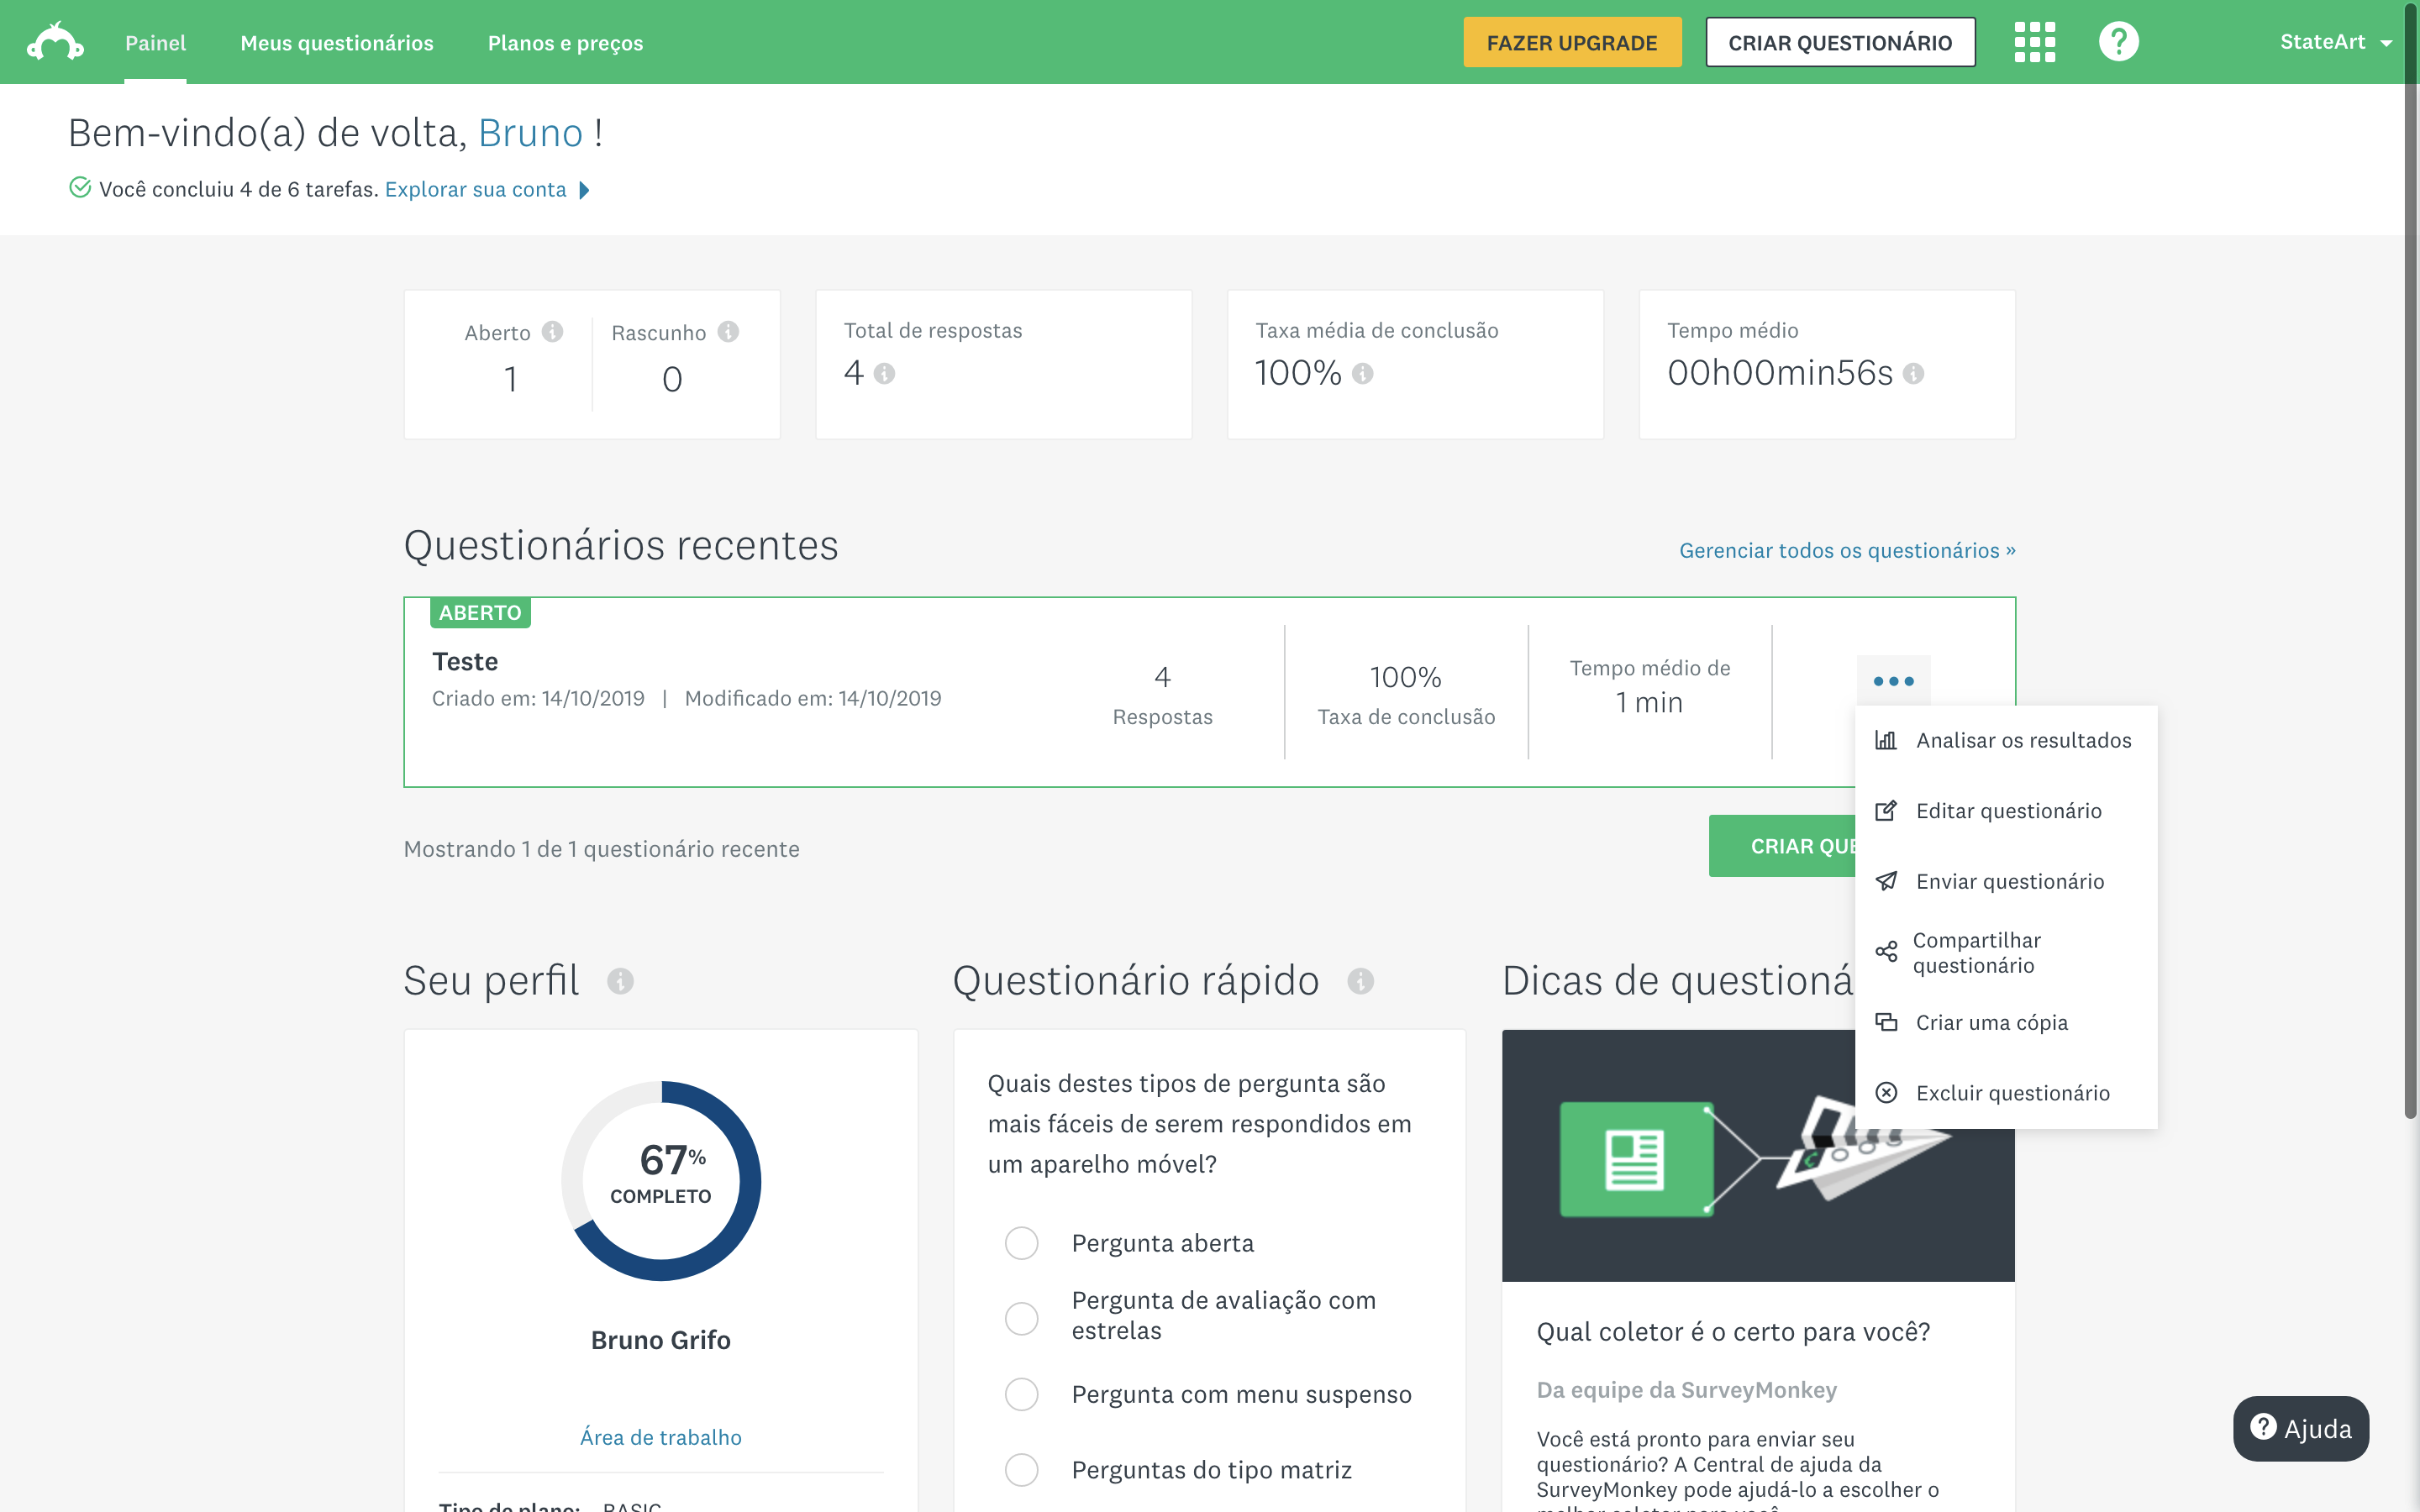
\includegraphics[width=1\textwidth]{img/sm/survey-dashboard}
		\caption{SurveyMonkey - Painel de Controle }
		\label{fig:survey-dashboard}
	\end{center}
\end{figure}

\newpage

\begin{figure}[ht!]
	\begin{center}
		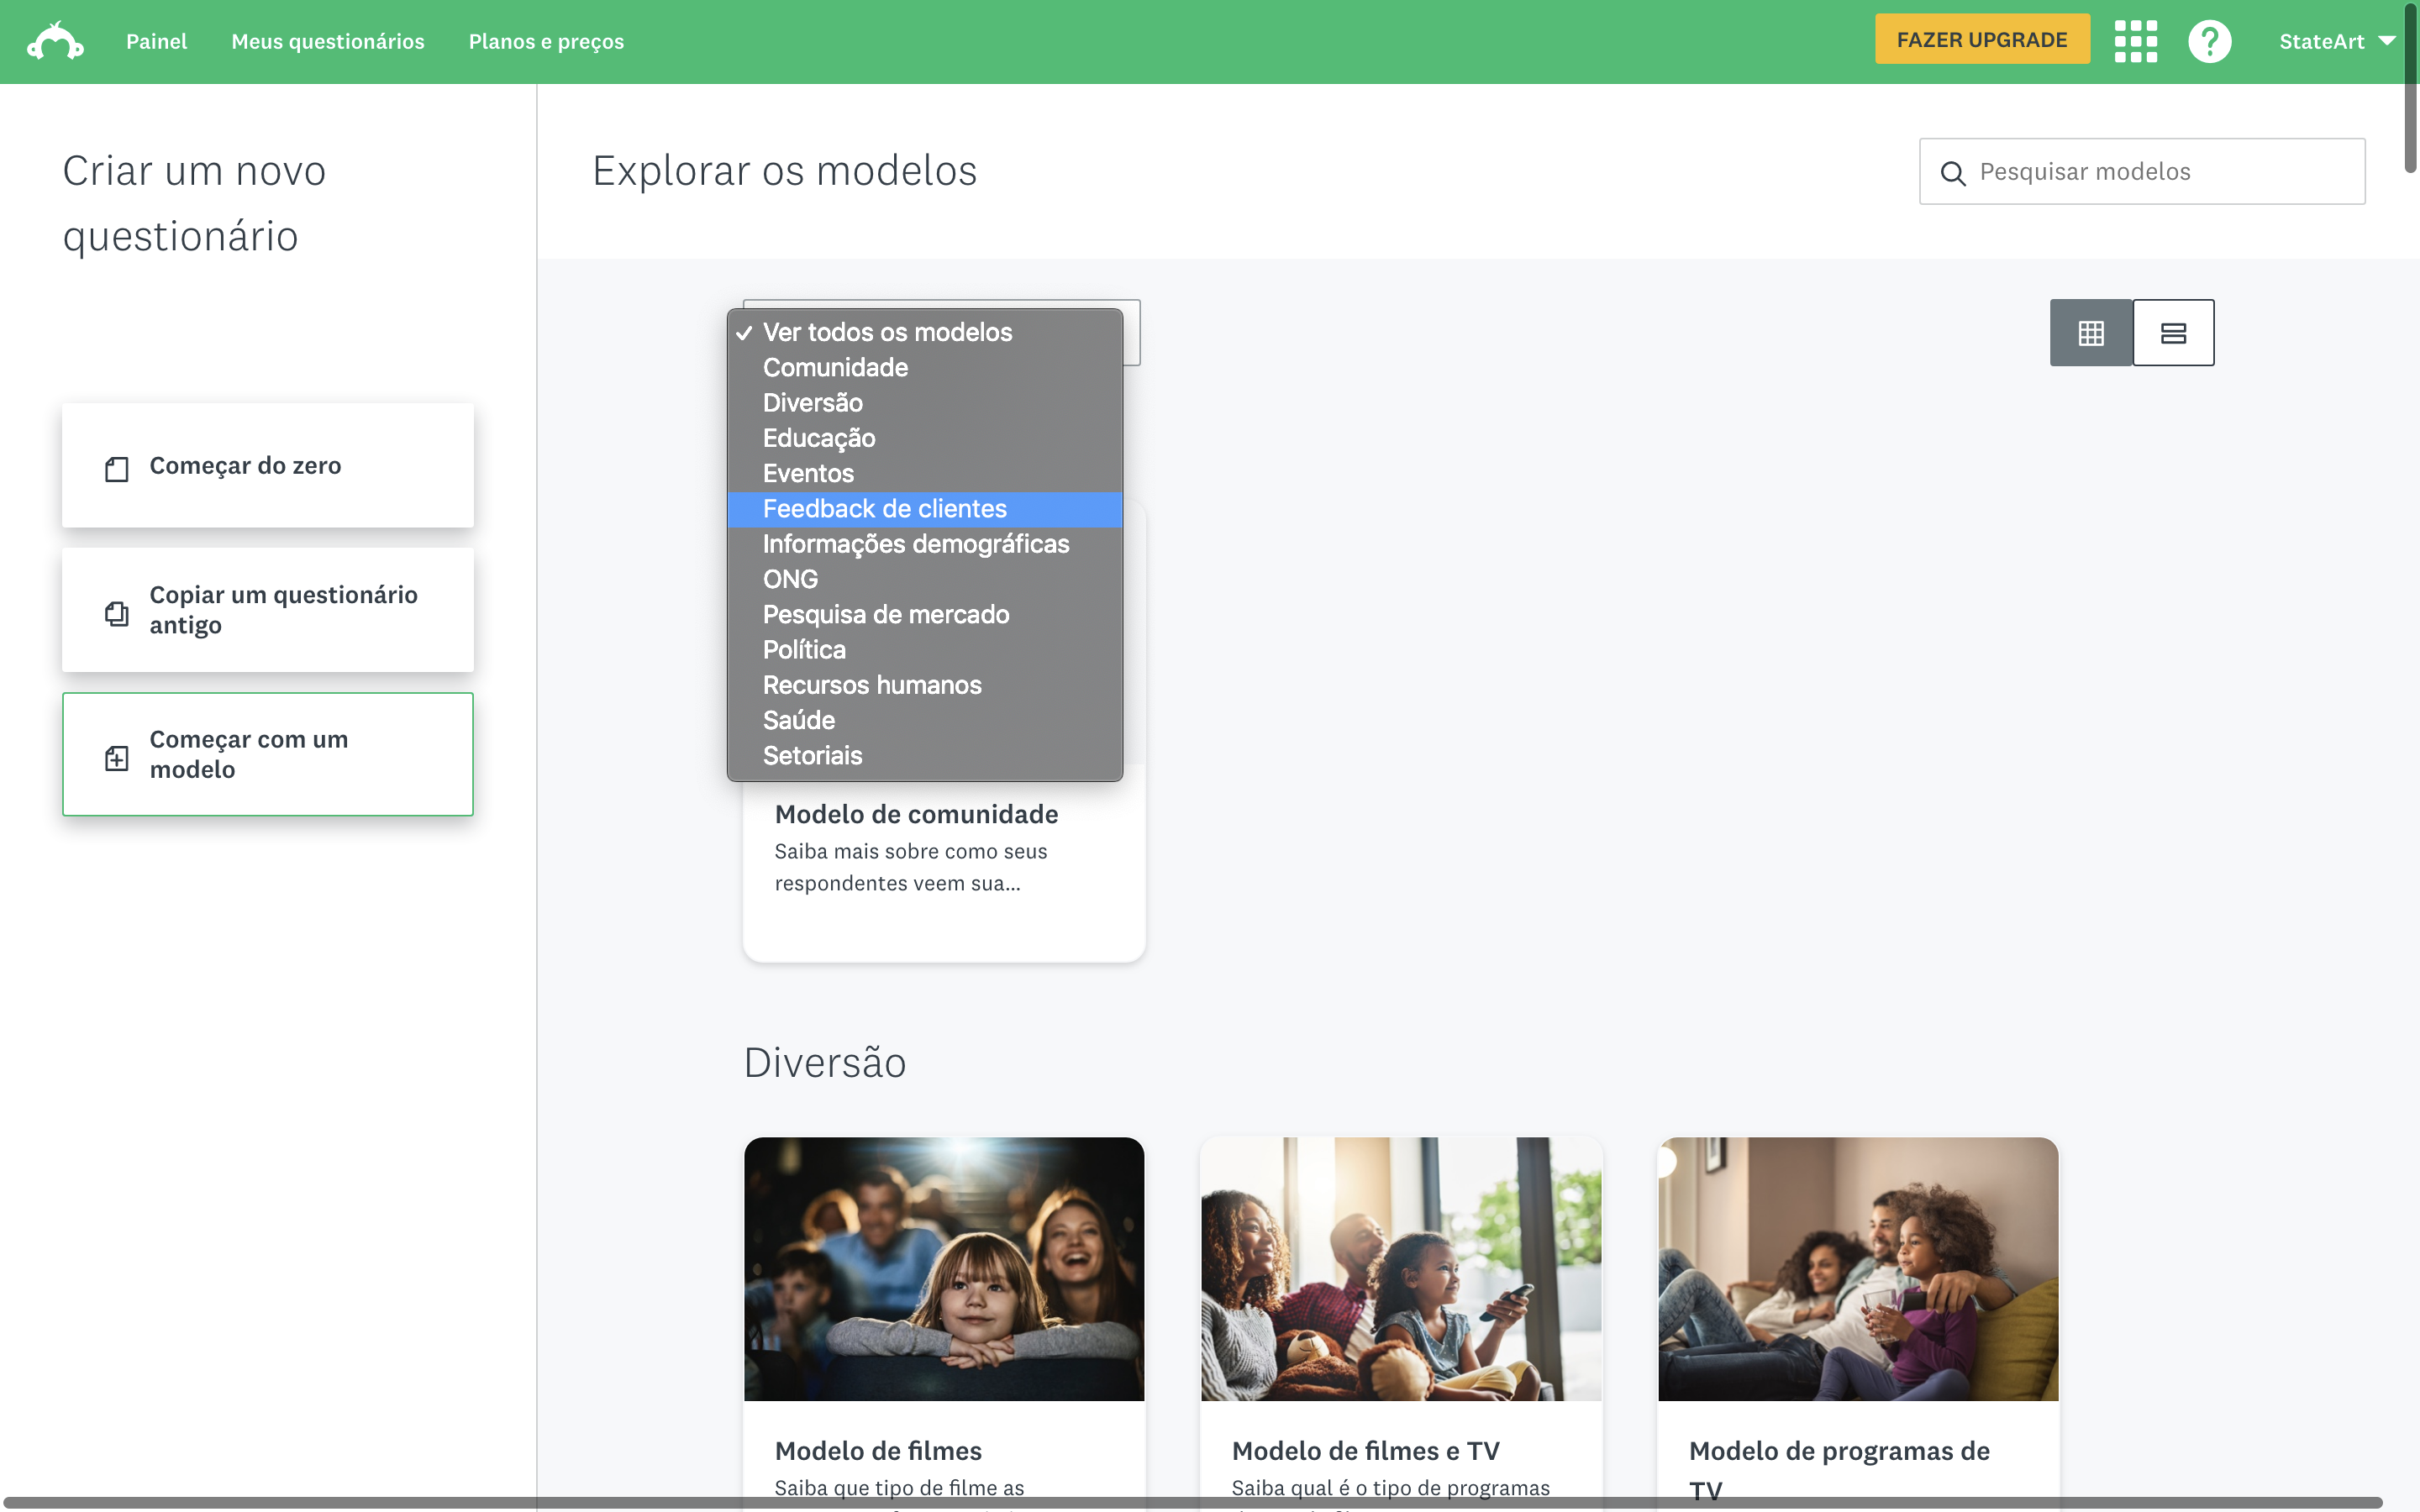
\includegraphics[width=1\textwidth]{img/sm/survey-form-create}
		\caption{SurveyMonkey - Formulários modelo }
		\label{fig:survey-form-create}
	\end{center}
\end{figure}

Quando se inicializa a criação de um novo formulário, a plataforma dá opção de começar do zero ou de utilizar um formulário modelo como podemos ver na Figura \ref{fig:survey-form-create}. Começando um formulário do zero como podemos ver na Figura \ref{fig:survey-form-banck2}, temos acesso a uma série de funcionalidades que vamos explorar e analisar em seguida.

\begin{figure}[ht!]
	\begin{center}
		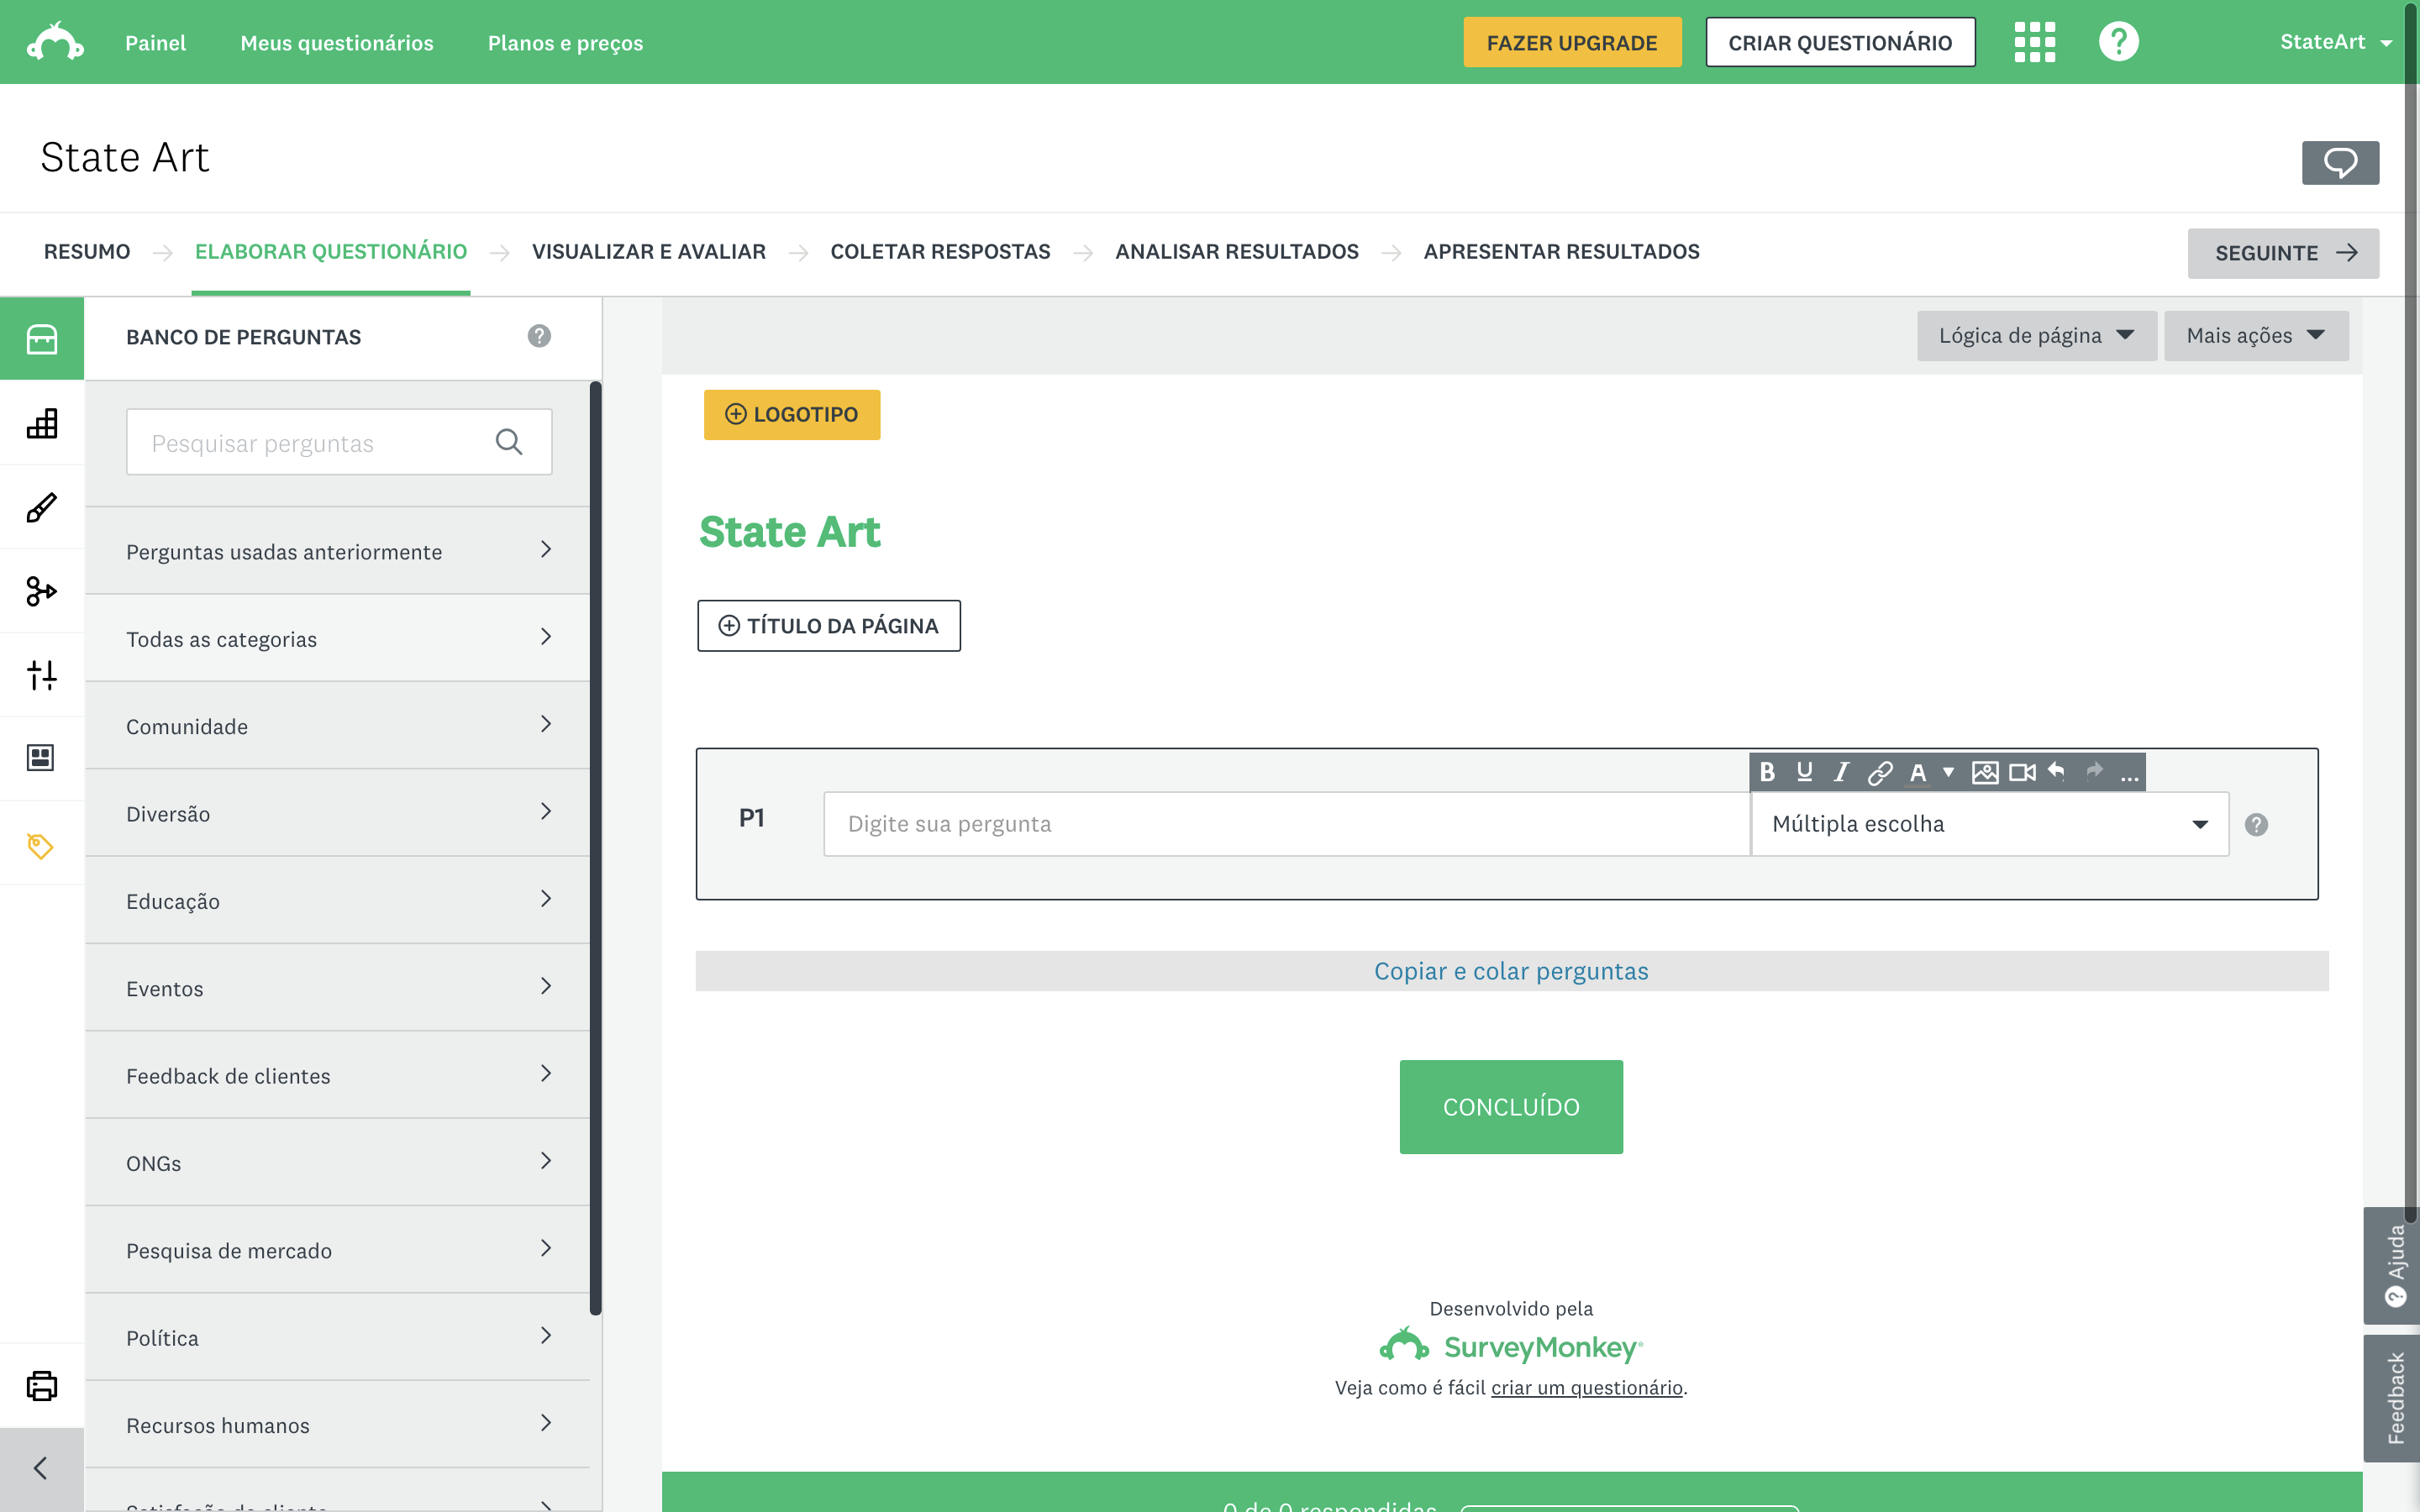
\includegraphics[width=1\textwidth]{img/sm/survey-form-bank2}
		\caption{SurveyMonkey -  Perguntas Modelo}
		\label{fig:survey-form-banck2}
	\end{center}
\end{figure}


\begin{figure}[ht!]
	\begin{center}
		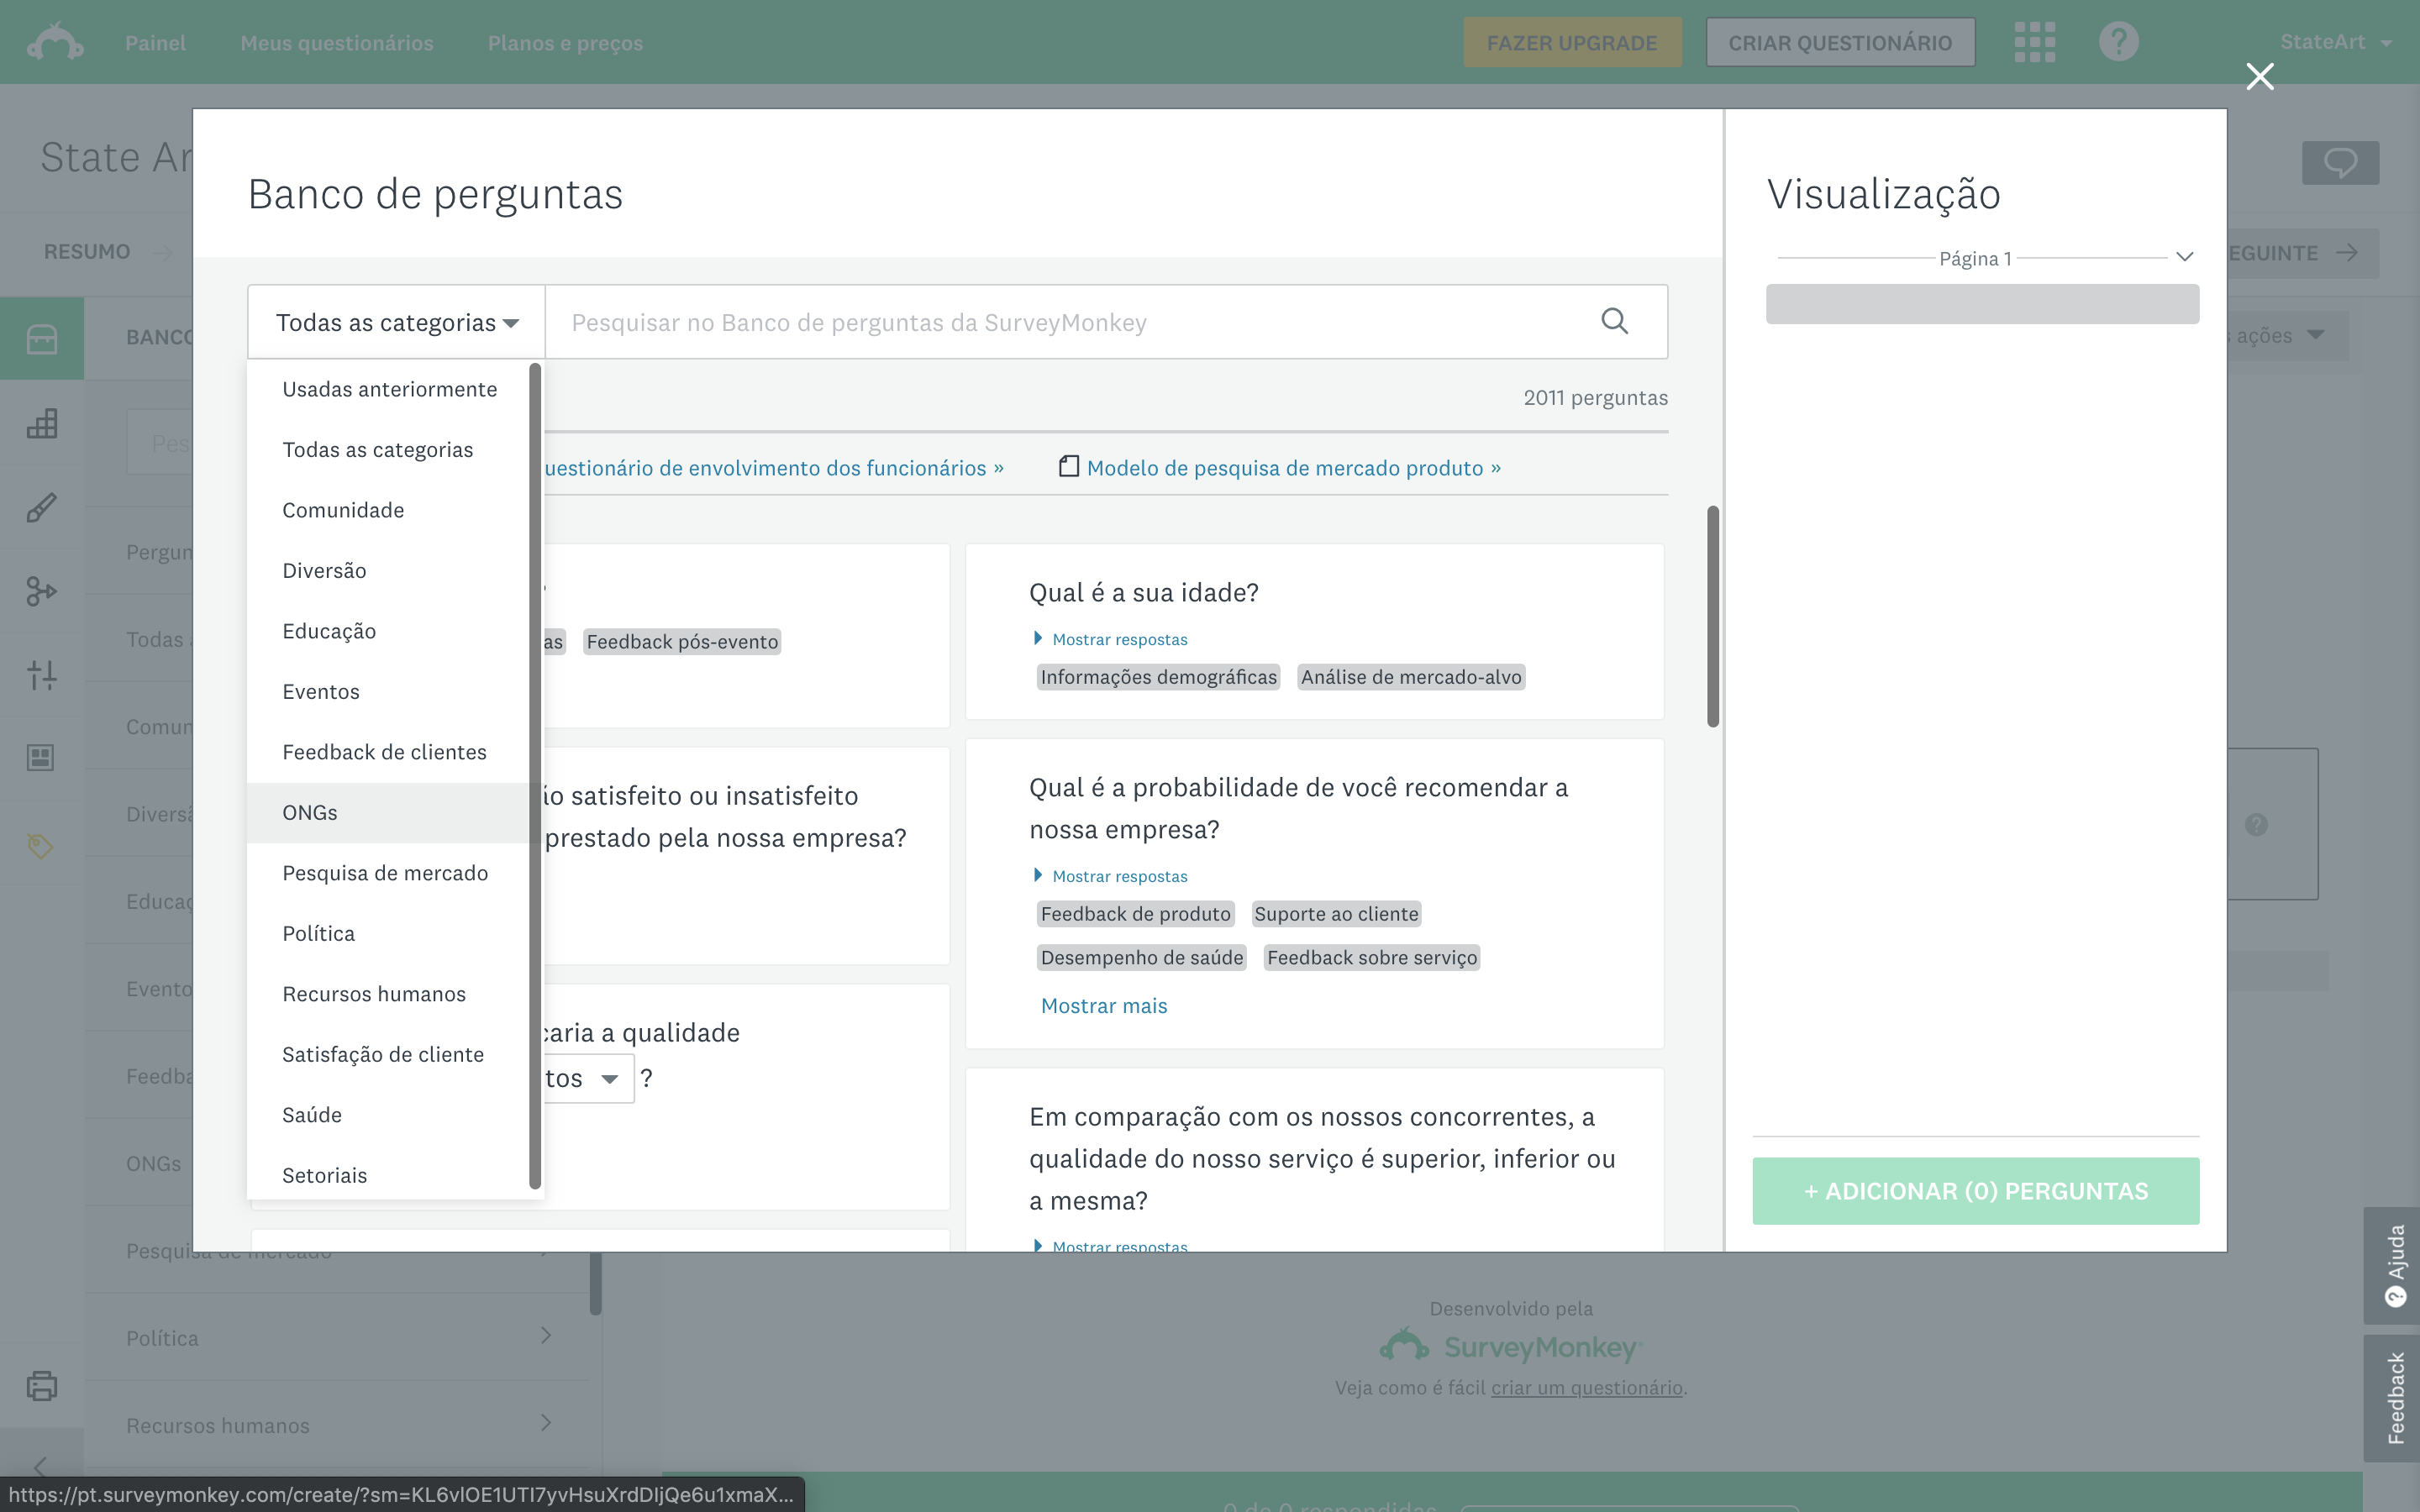
\includegraphics[width=1\textwidth]{img/sm/survey-form-bank1}
		\caption{SurveyMonkey - Perguntas Modelo }
		\label{fig:survey-form-banck1}
	\end{center}
\end{figure}

\newpage

São diversos os elementos que se podem adicionar ou arrastar para o formulário (i. e. perguntas, escolha multipla, imagens...) como representado na Figura \ref{fig:surveymonkey-form-element} e há também um banco de perguntas modelo/recomendações já construídas, organizadas por categorias como podemos ver na Figura \ref{fig:survey-form-banck2} e \ref{fig:survey-form-banck1}.


\begin{figure}[ht!]
	\begin{center}
		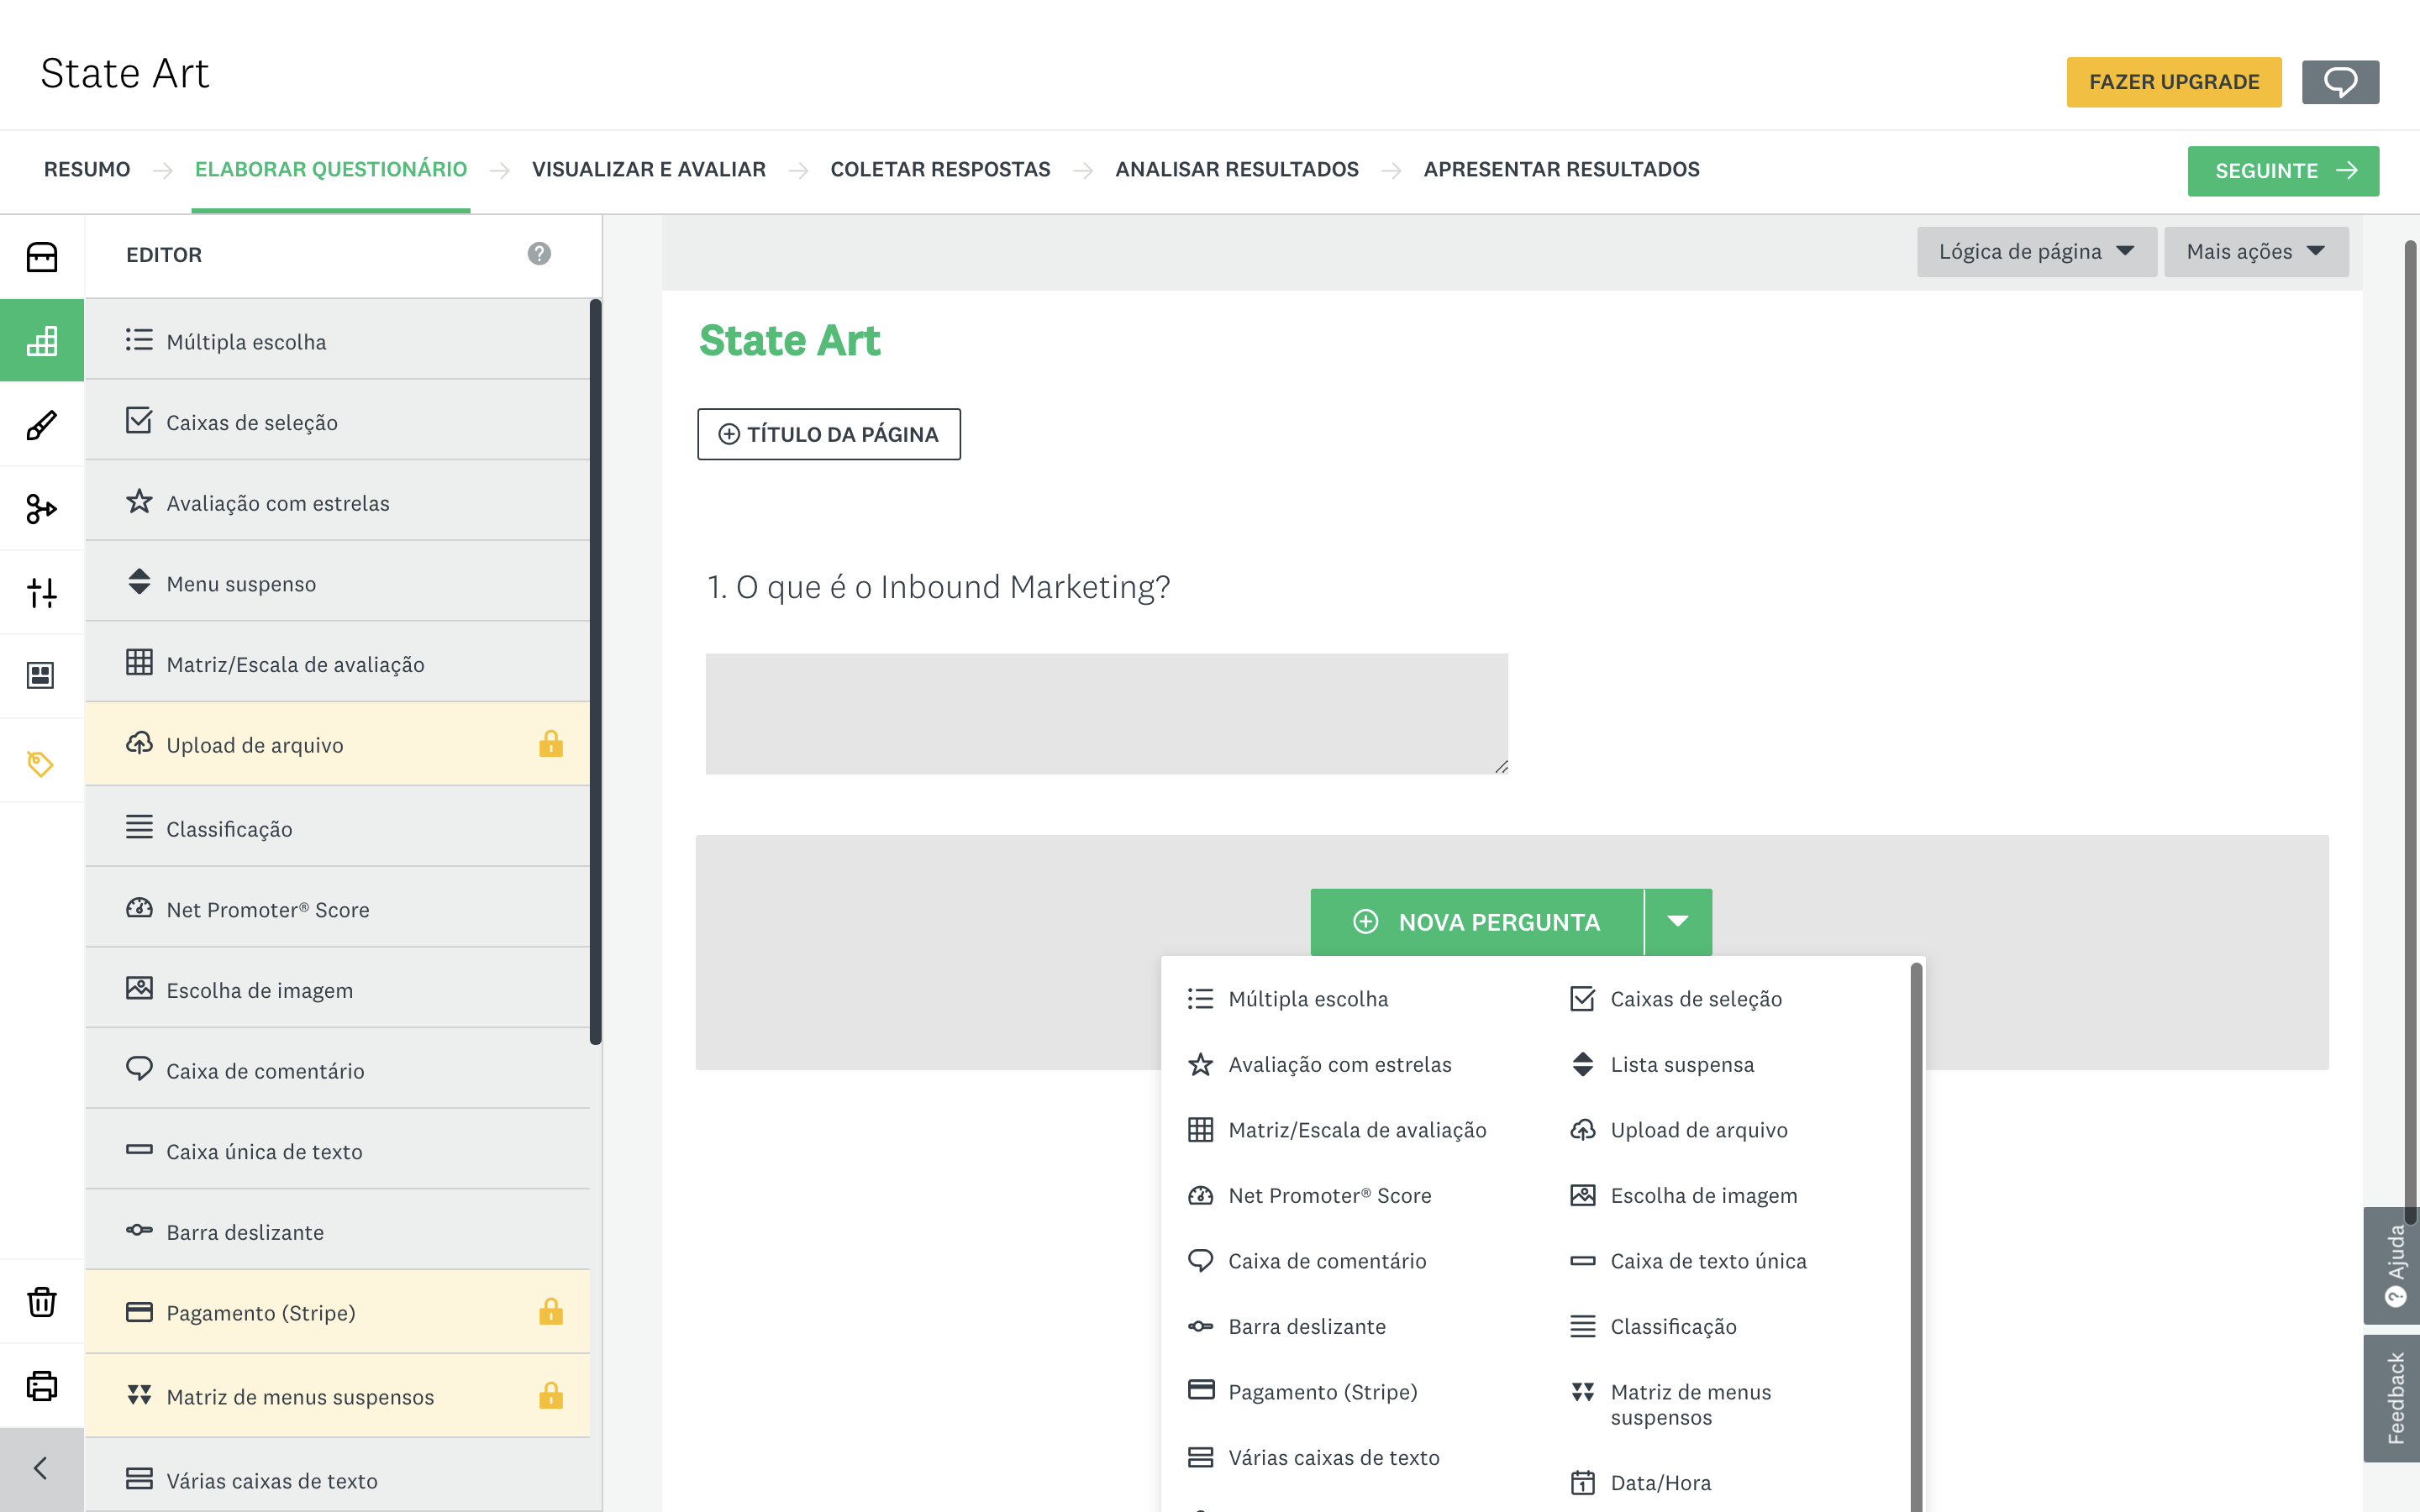
\includegraphics[width=1\textwidth]{img/sm/surveymonkey-form-element}
		\caption{SurveyMonkey - Elementos }
		\label{fig:surveymonkey-form-element}
	\end{center}
\end{figure}
\newpage

\begin{figure}[ht!]
	\begin{center}
		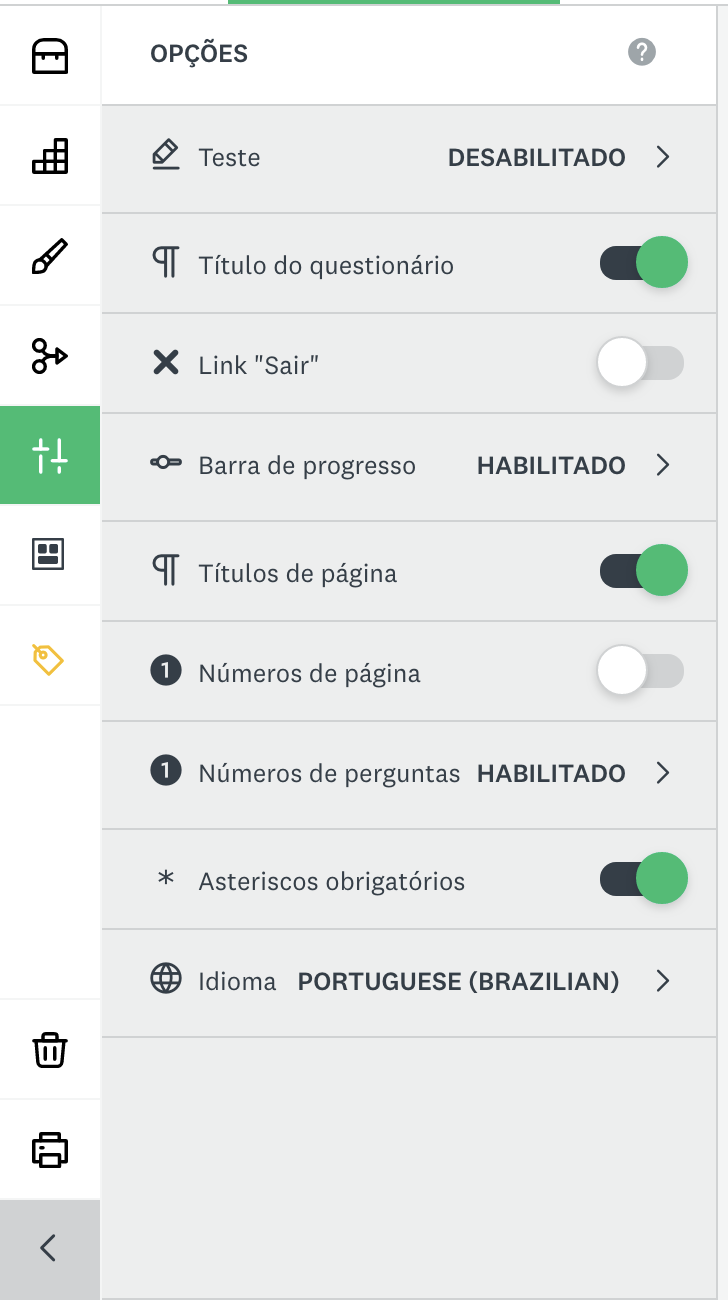
\includegraphics[height=.35\textheight]{img/sm/surveymonkey-form-opcoes}
		\caption{SurveyMonkey - Opções}
		\label{fig:surveymonkey-form-opcoes}
	\end{center}
\end{figure}

\begin{figure}[ht!]
	\begin{center}
		\begin{minipage}{0.45\textwidth}
			\begin{center}
				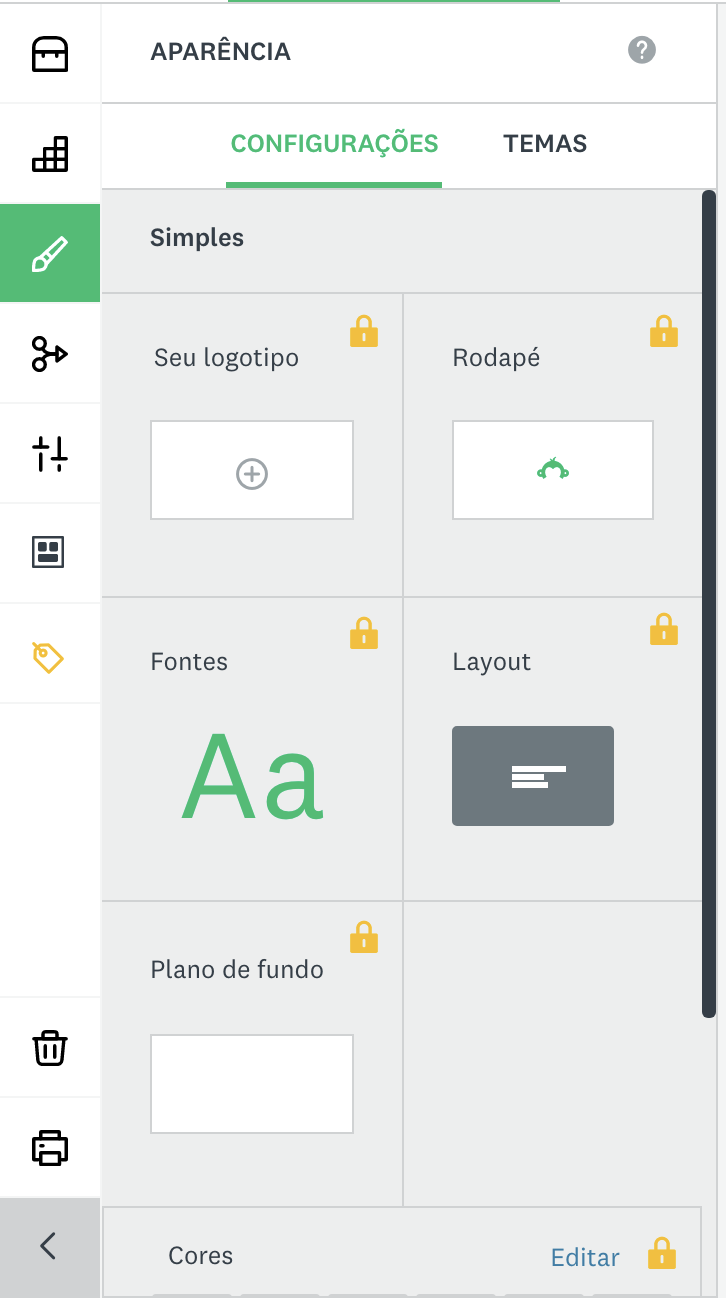
\includegraphics[height=.35\textheight]{img/sm/surveymonkey-form-aparencia}
				\caption{SurveyMonkey - Aparência}
				\label{fig:surveymonkey-form-aparencia}
			\end{center}
		\end{minipage}
		\hspace{1cm}
		\begin{minipage}{0.45\textwidth}
			\begin{center}
				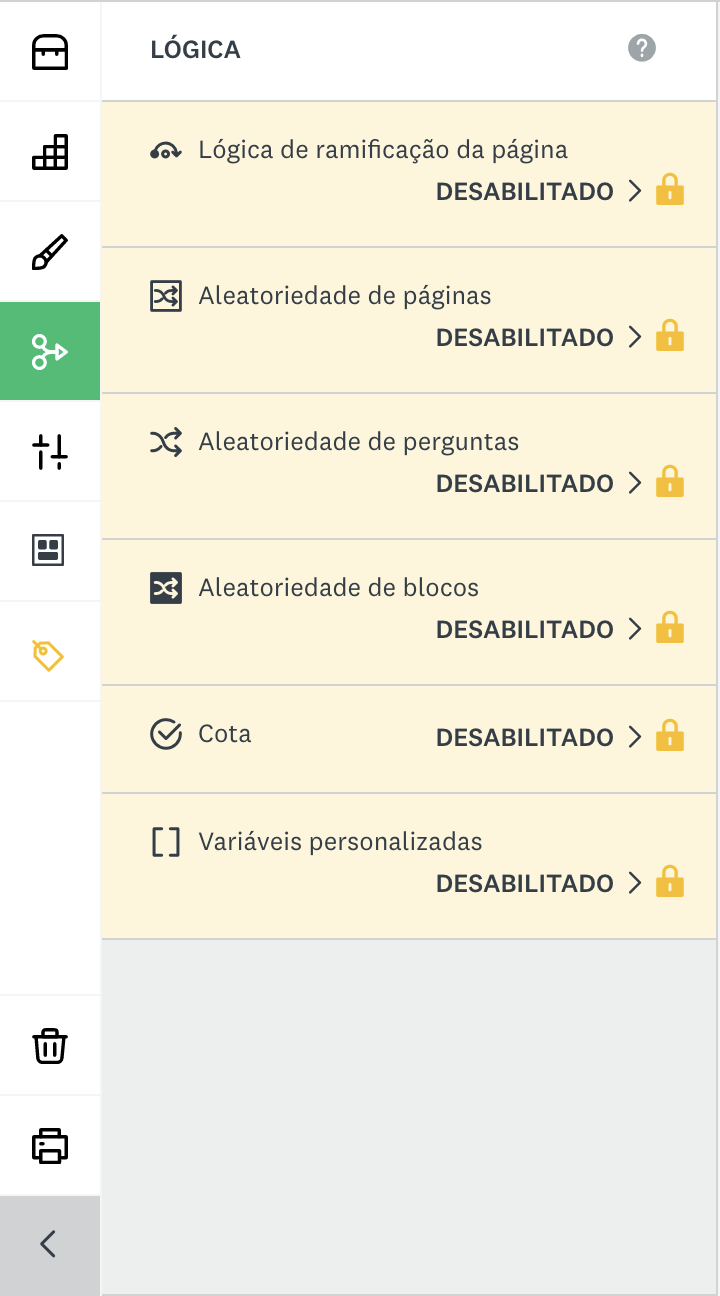
\includegraphics[height=.35\textheight]{img/sm/surveymonkey-form-logica}
				\caption{SurveyMonkey - Lógica}
				\label{fig:surveymonkey-form-logica}
			\end{center}
		\end{minipage}
	\end{center}
\end{figure}

O SurveyMonkey permite também realizar algumas operações de personalização do formulário. Nas Figuras \ref{fig:surveymonkey-form-opcoes}, \ref{fig:surveymonkey-form-aparencia} e \ref{fig:surveymonkey-form-logica} estão representaçãs as opções, aparência e lógica do formulário, respetivamente, que permite costumizar formulários ao público alvo. 
Depois de realizado o formulário esta plataforma permite a visualização do mesmo, em diferentes tipos de dispositivos, como se pode ver nas Figuras \ref{fig:surveymonkey-form-test-pc} e \ref{fig:surveymonkey-form-test-phone}, para verificar se tudo está conforme planeado para se poder prosseguir para a recolha de dados. 
 \newpage

\begin{figure}[ht!]
	\begin{center}
		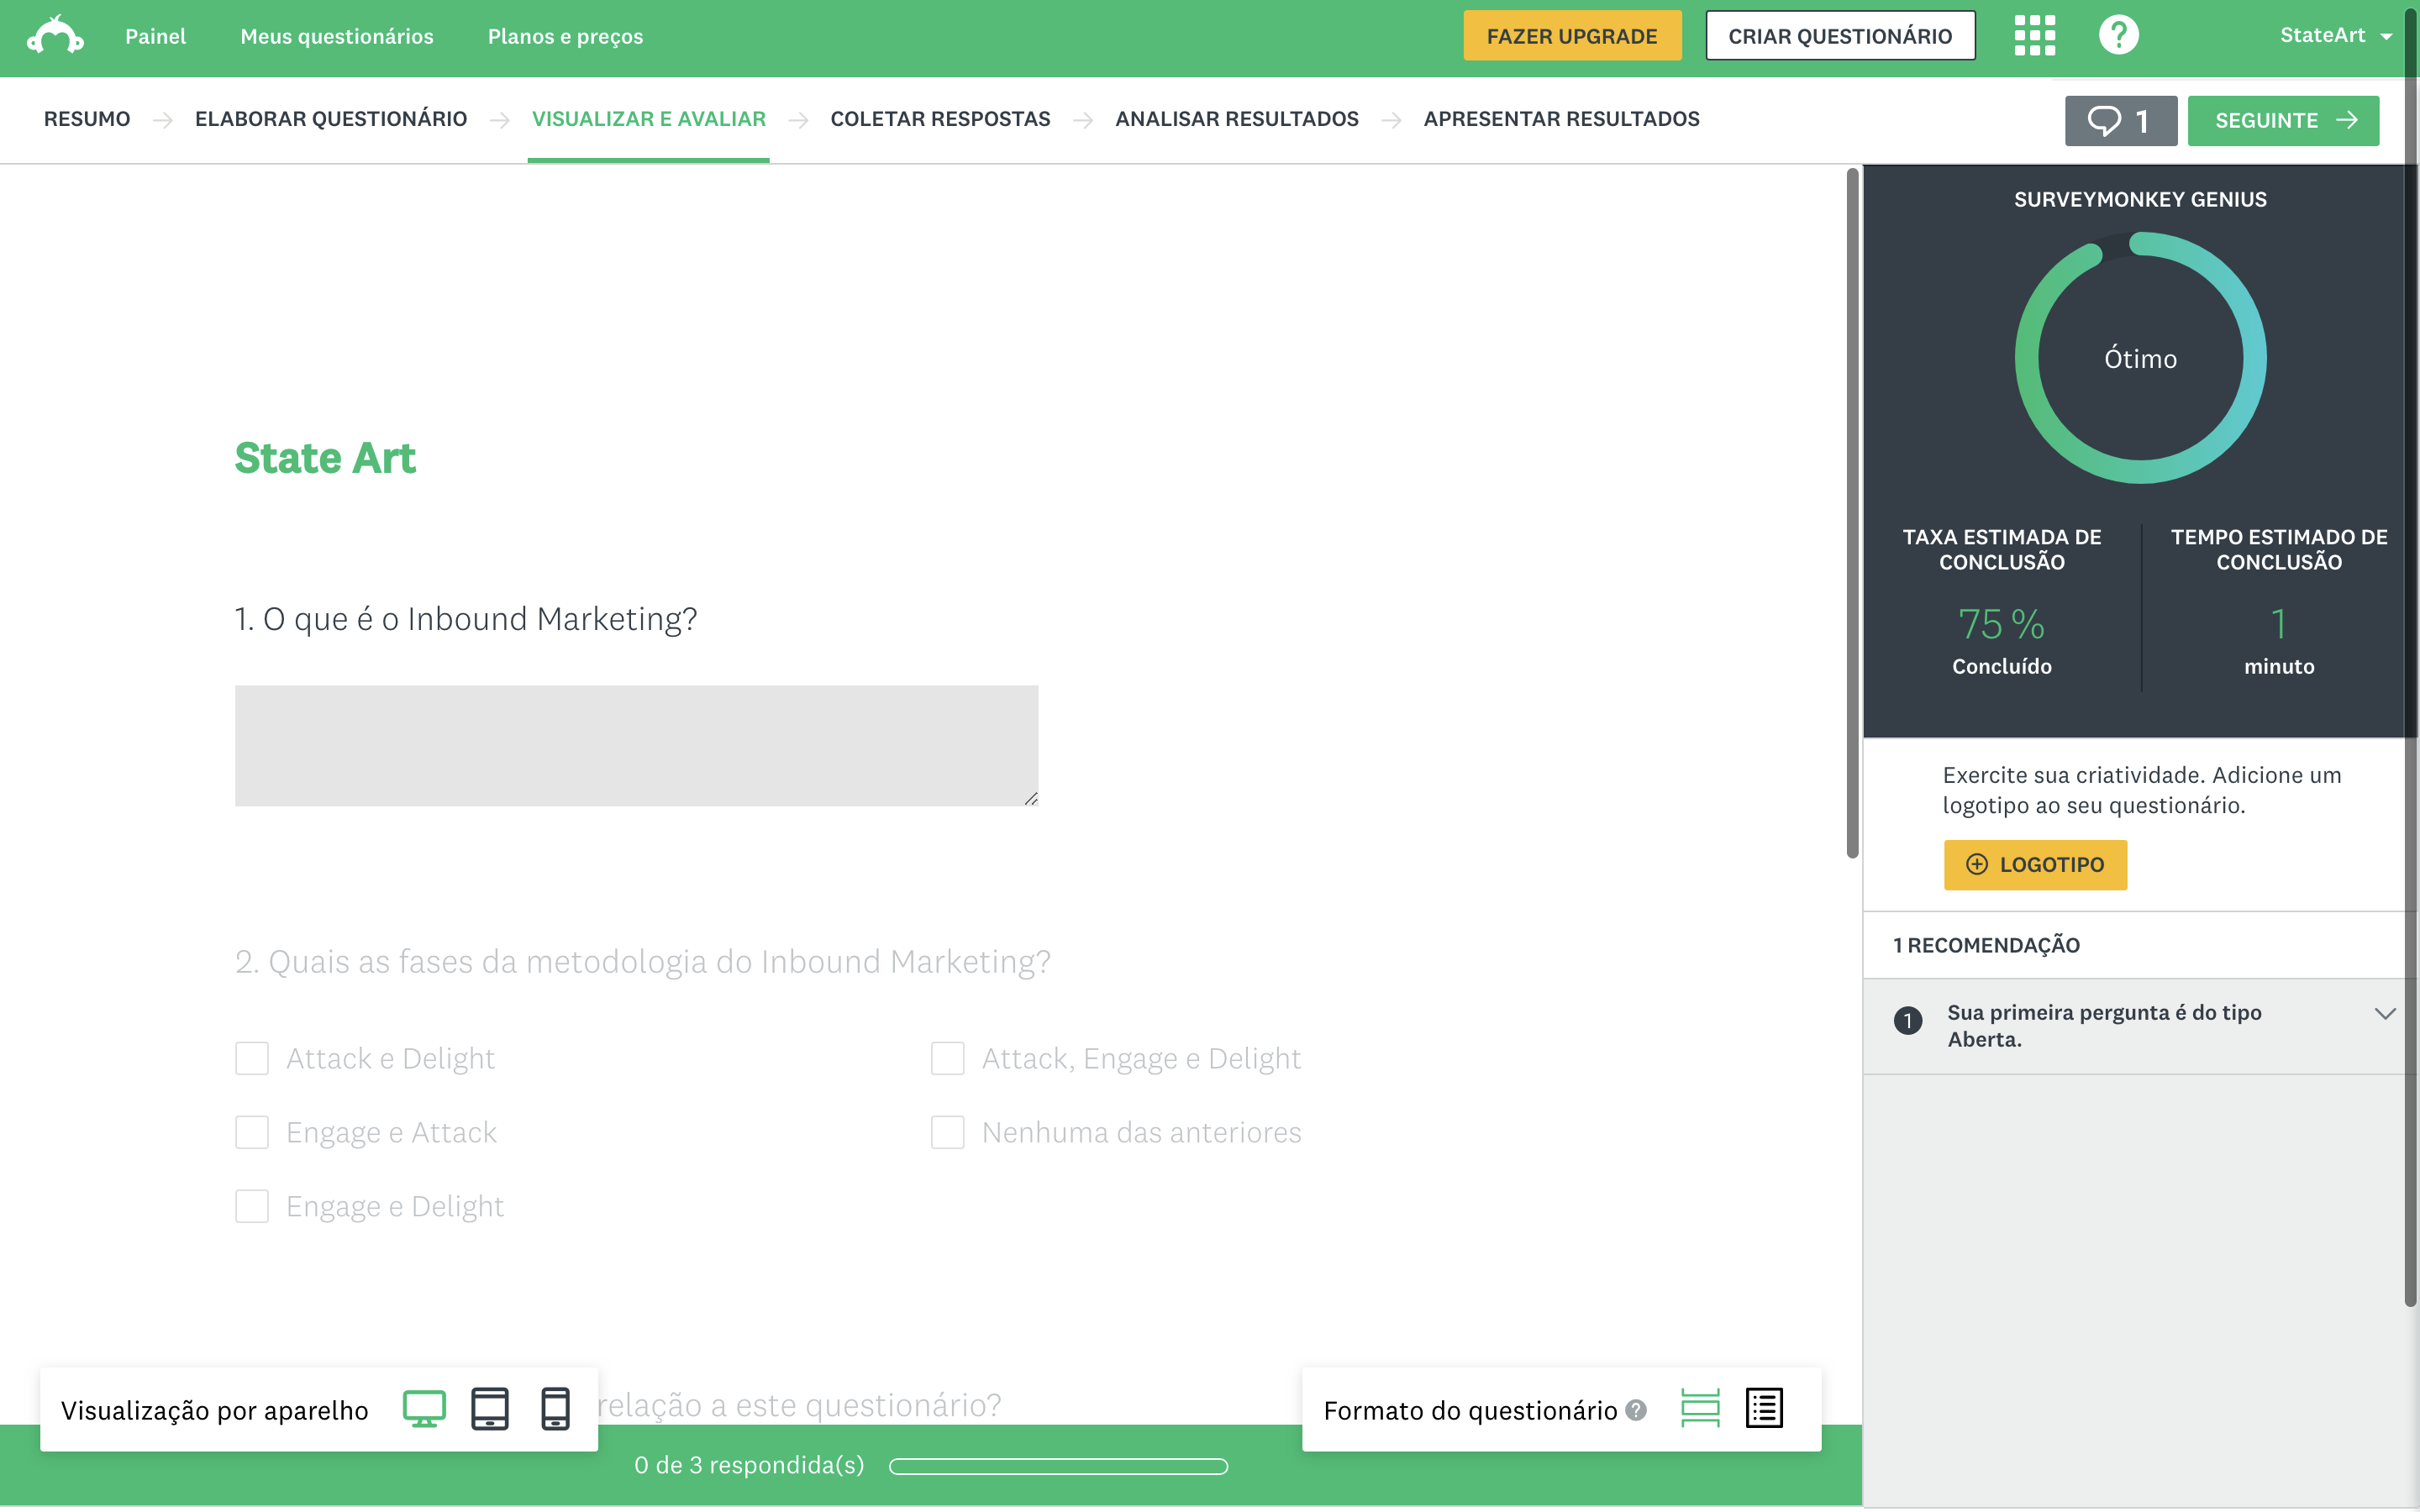
\includegraphics[width=1\textwidth]{img/sm/surveymonkey-form-test-pc}
		\caption{SurveyMonkey - Visualização do formulário em computador }
		\label{fig:surveymonkey-form-test-pc}
	\end{center}
\end{figure}

\begin{figure}[ht!]
	\begin{center}
		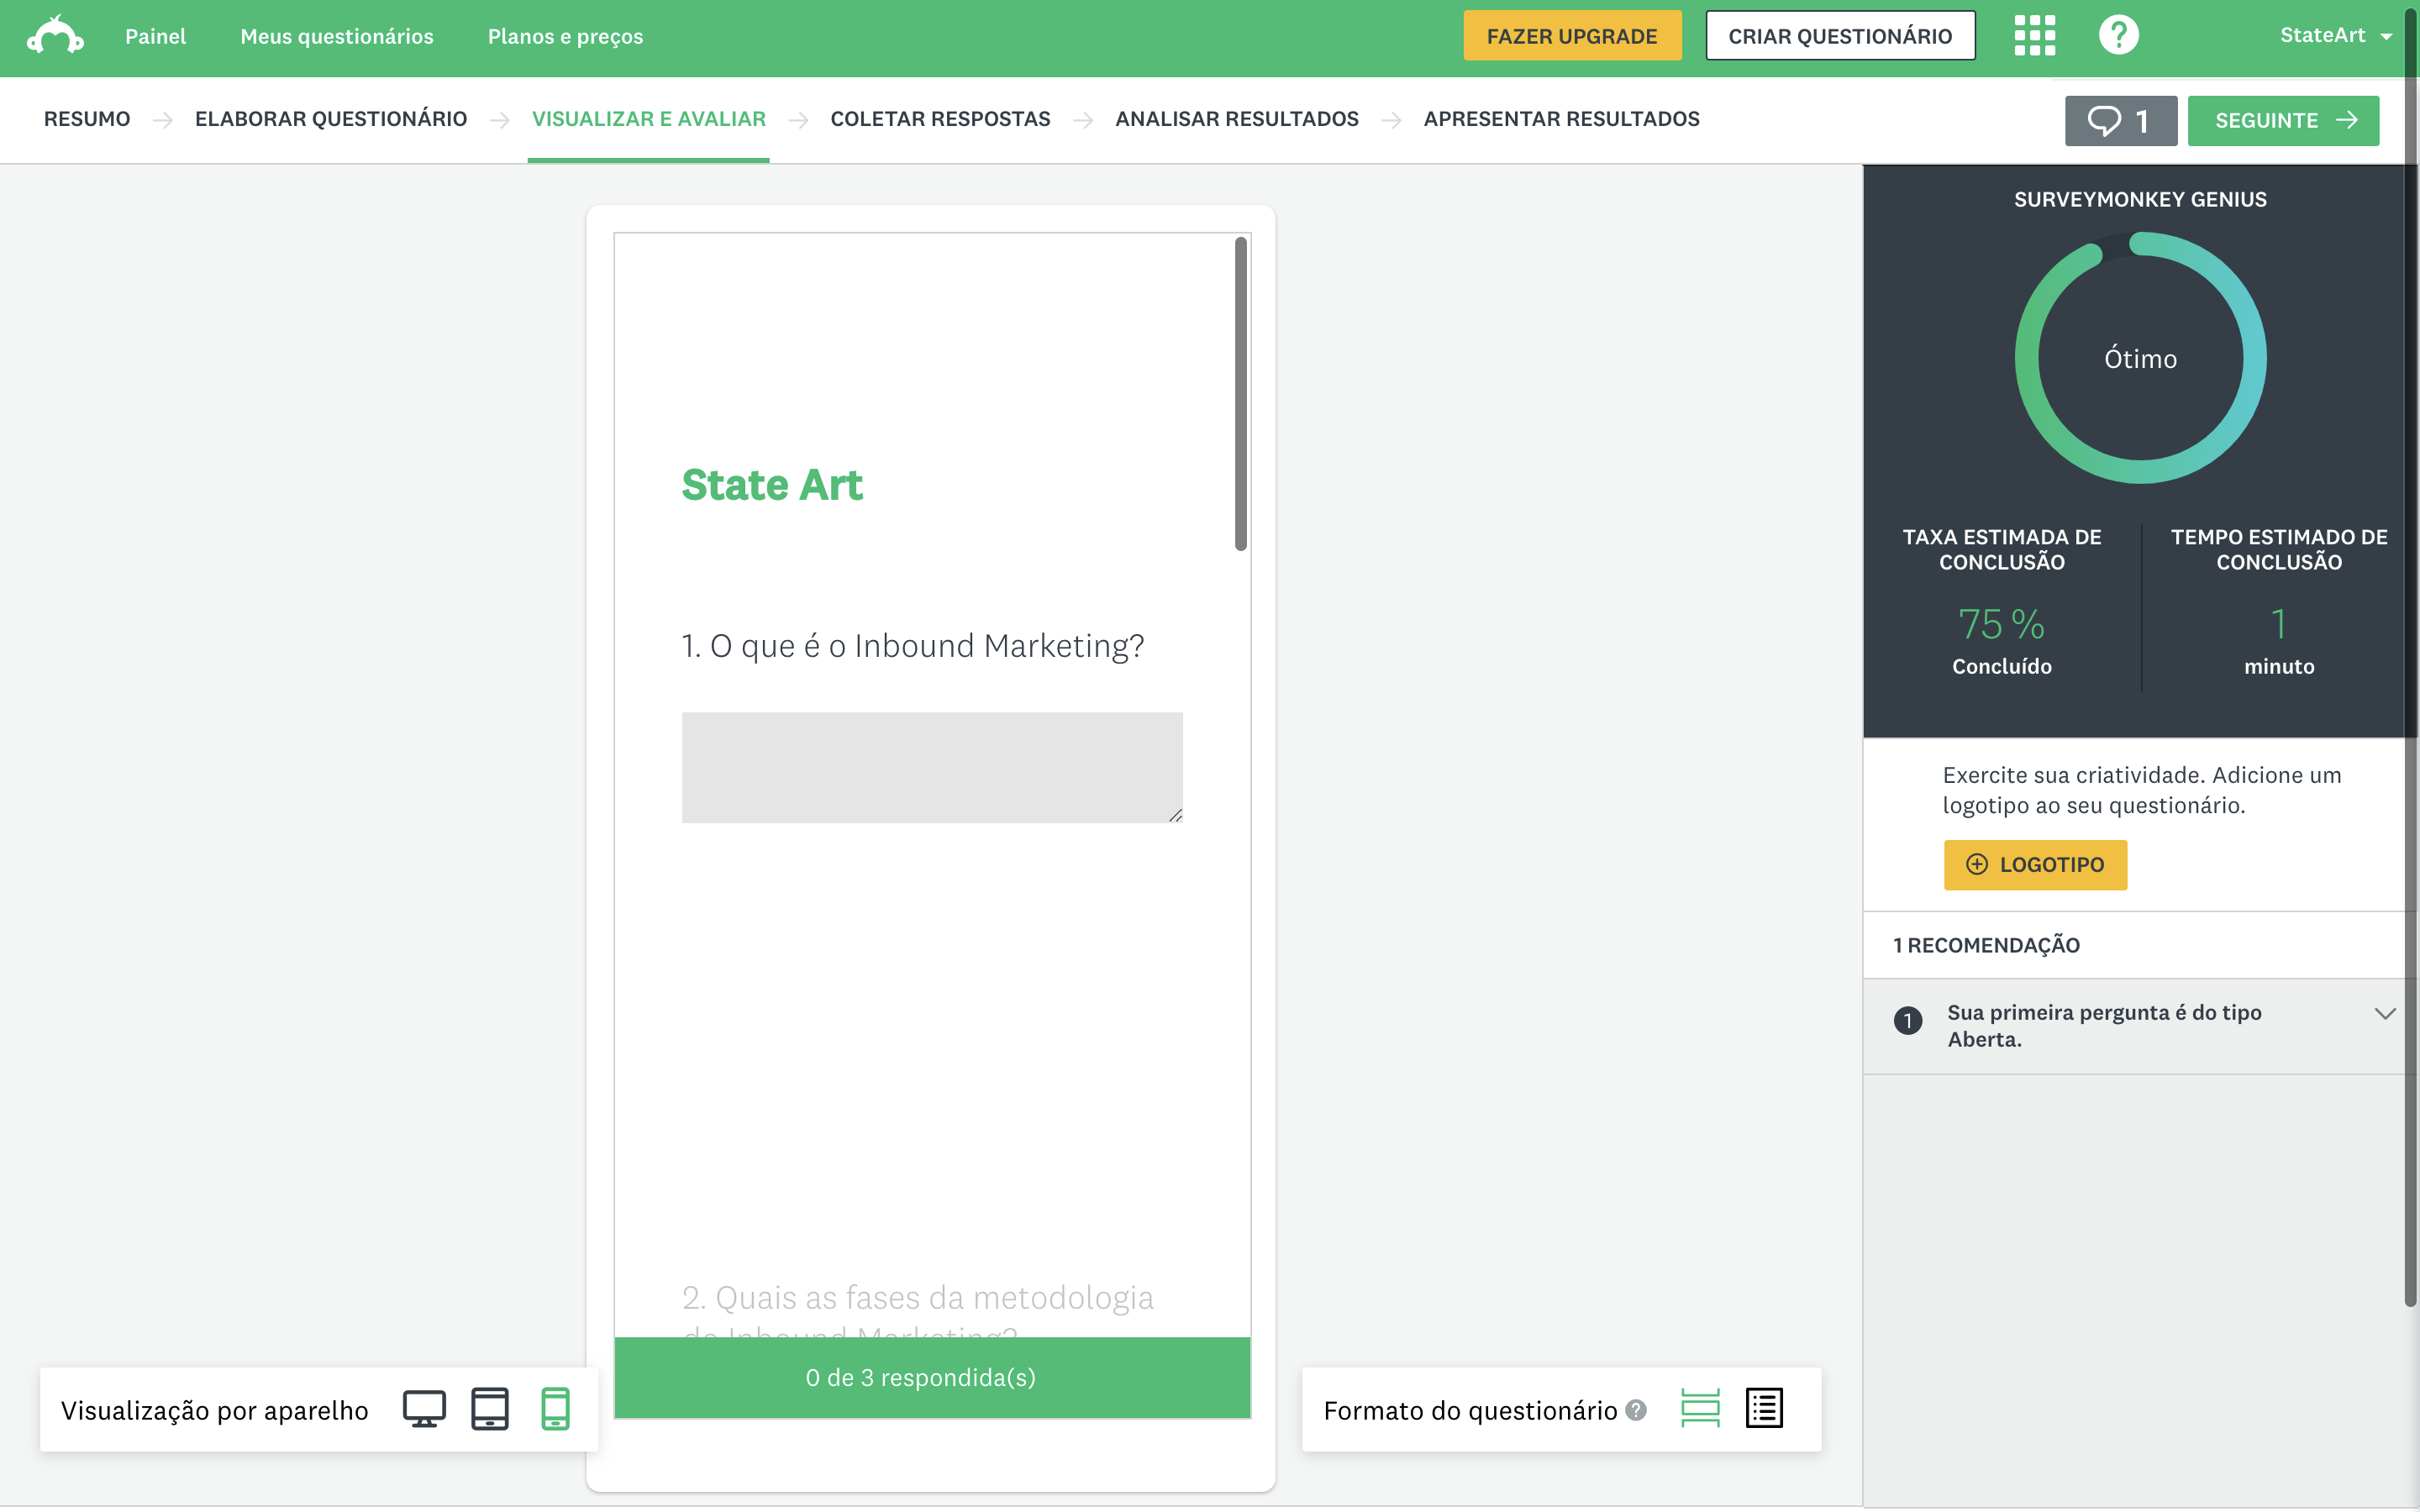
\includegraphics[width=1\textwidth]{img/sm/surveymonkey-form-test-phone}
		\caption{SurveyMonkey - Visualisação do formulário em smartphone }
		\label{fig:surveymonkey-form-test-phone}
	\end{center}
\end{figure}

Depois de garantir que o formulário foi construido como desejado a plataforma fornece vários meios pelo qual se pode partilhar/enviar o formulário, como listado na Figura \ref{fig:surveymonkey-form-share}.

\newpage

\begin{figure}[ht!]
	\begin{center}
		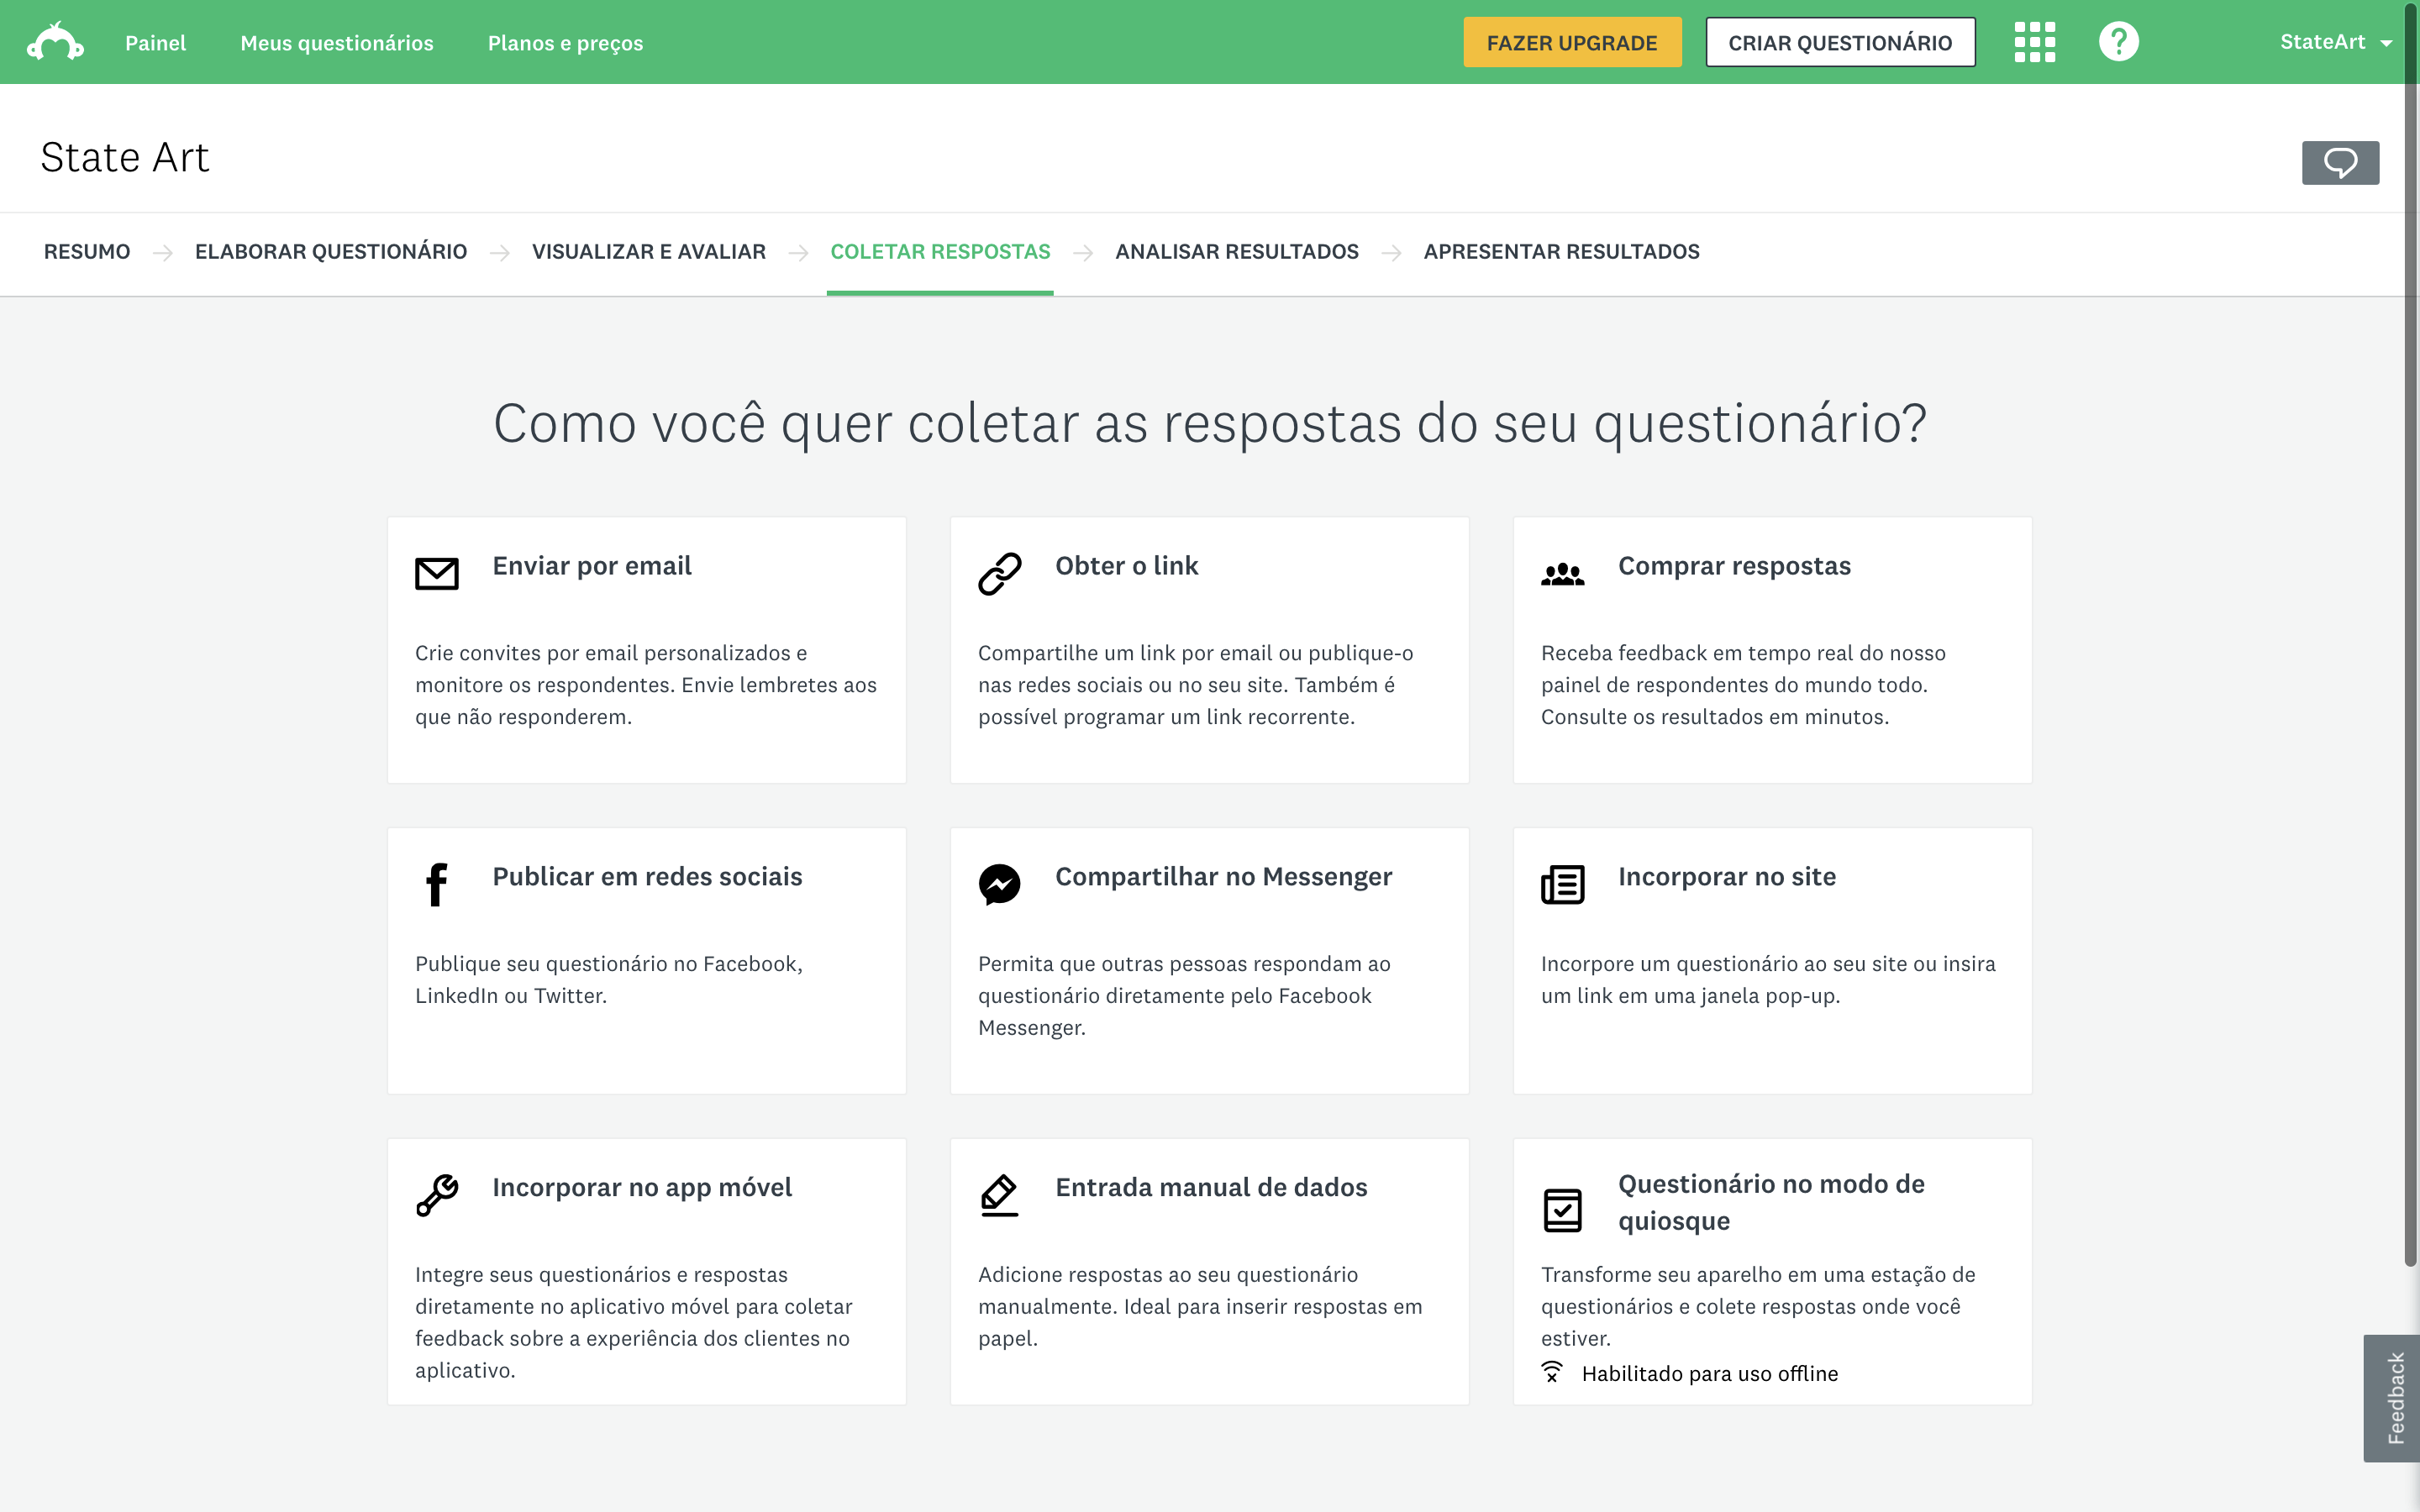
\includegraphics[width=1\textwidth]{img/sm/surveymonkey-form-share}
		\caption{SurveyMonkey - Metodo de partilha do formulário }
		\label{fig:surveymonkey-form-share}
	\end{center}
\end{figure}

Na analise de resultados, é necessário actualizar a página ou aplicar um filtro para que os gráficos e as estatísticas sejam actualizadas. 
O mesmo se passa na página que pode ser gerada para partilhar o sumário dos dados recolhidos, através do formulário. 
Para aplicar um filtro é necessário escolher o tipo de filtro e os elementos ao qual queremos aplicar o filtro como podemos ver nas Figuras \ref{fig:surveymonkey-form-filtro} e \ref{fig:surveymonkey-form-filtro1}. 


\begin{figure}[ht!]
	\begin{center}
		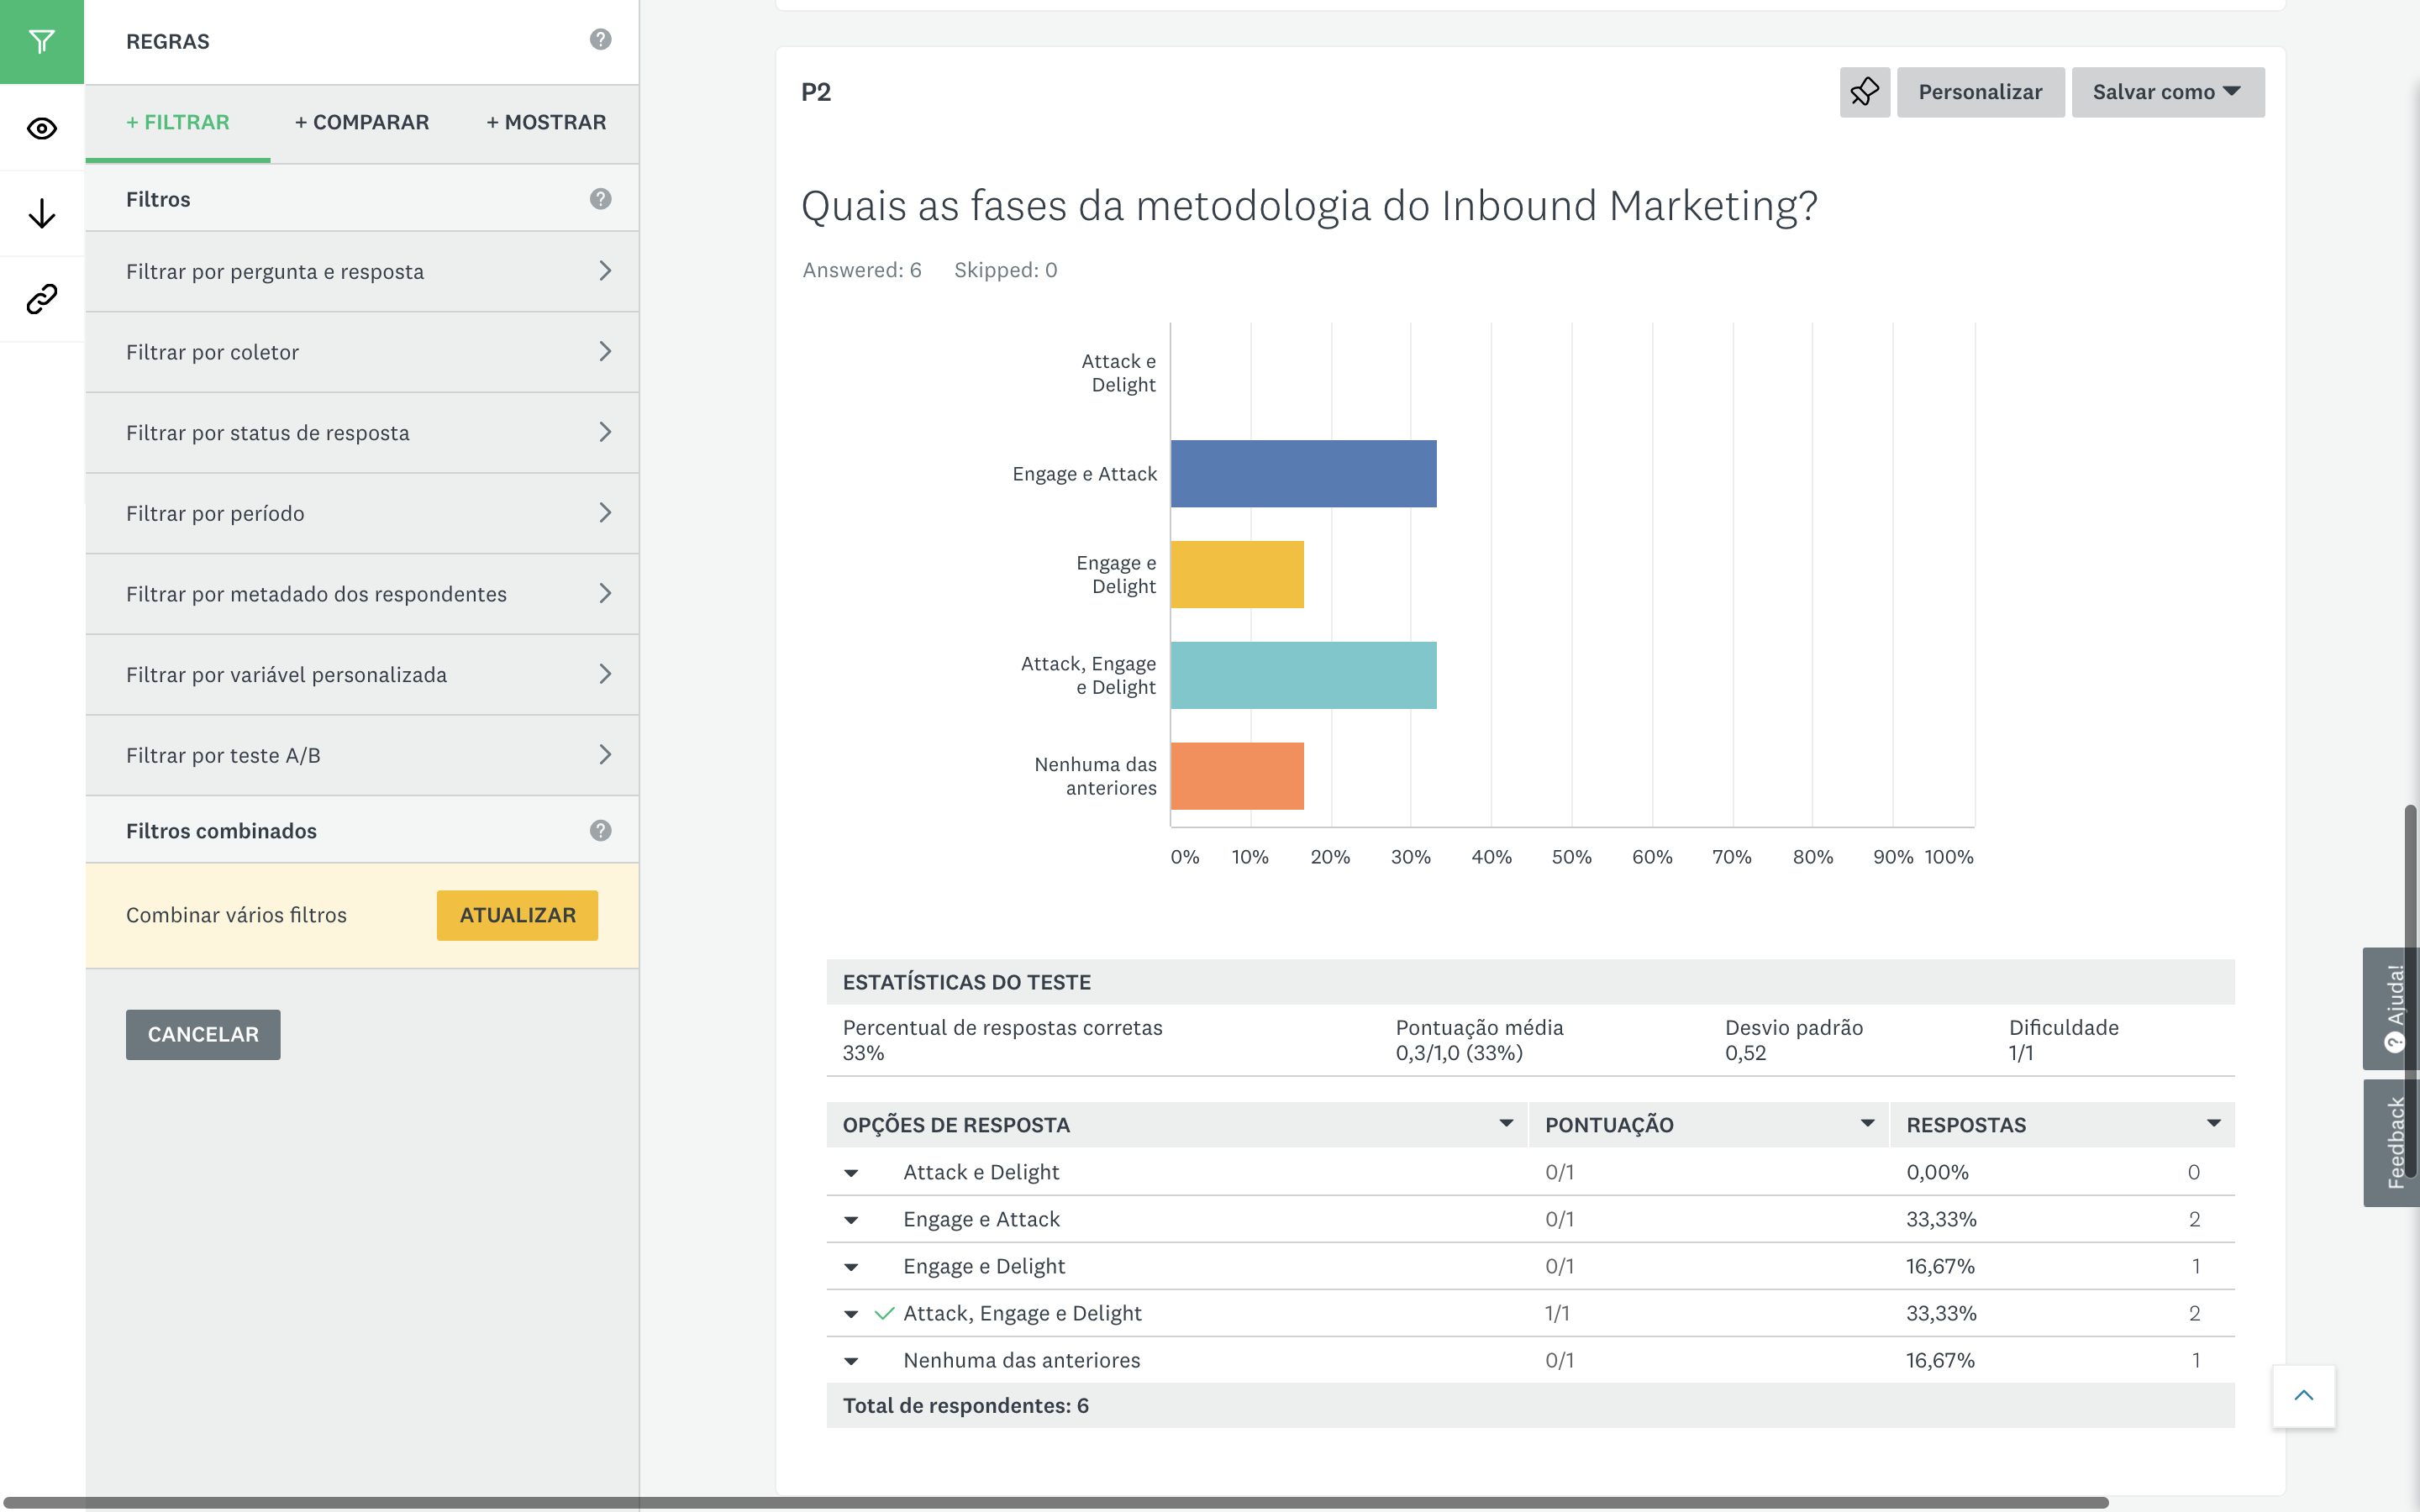
\includegraphics[width=1\textwidth]{img/sm/surveymonkey-form-filtro}
		\caption{SurveyMonkey - Tipos de Filtros }
		\label{fig:surveymonkey-form-filtro}
	\end{center}
\end{figure}



\begin{figure}[ht!]
	\begin{center}
		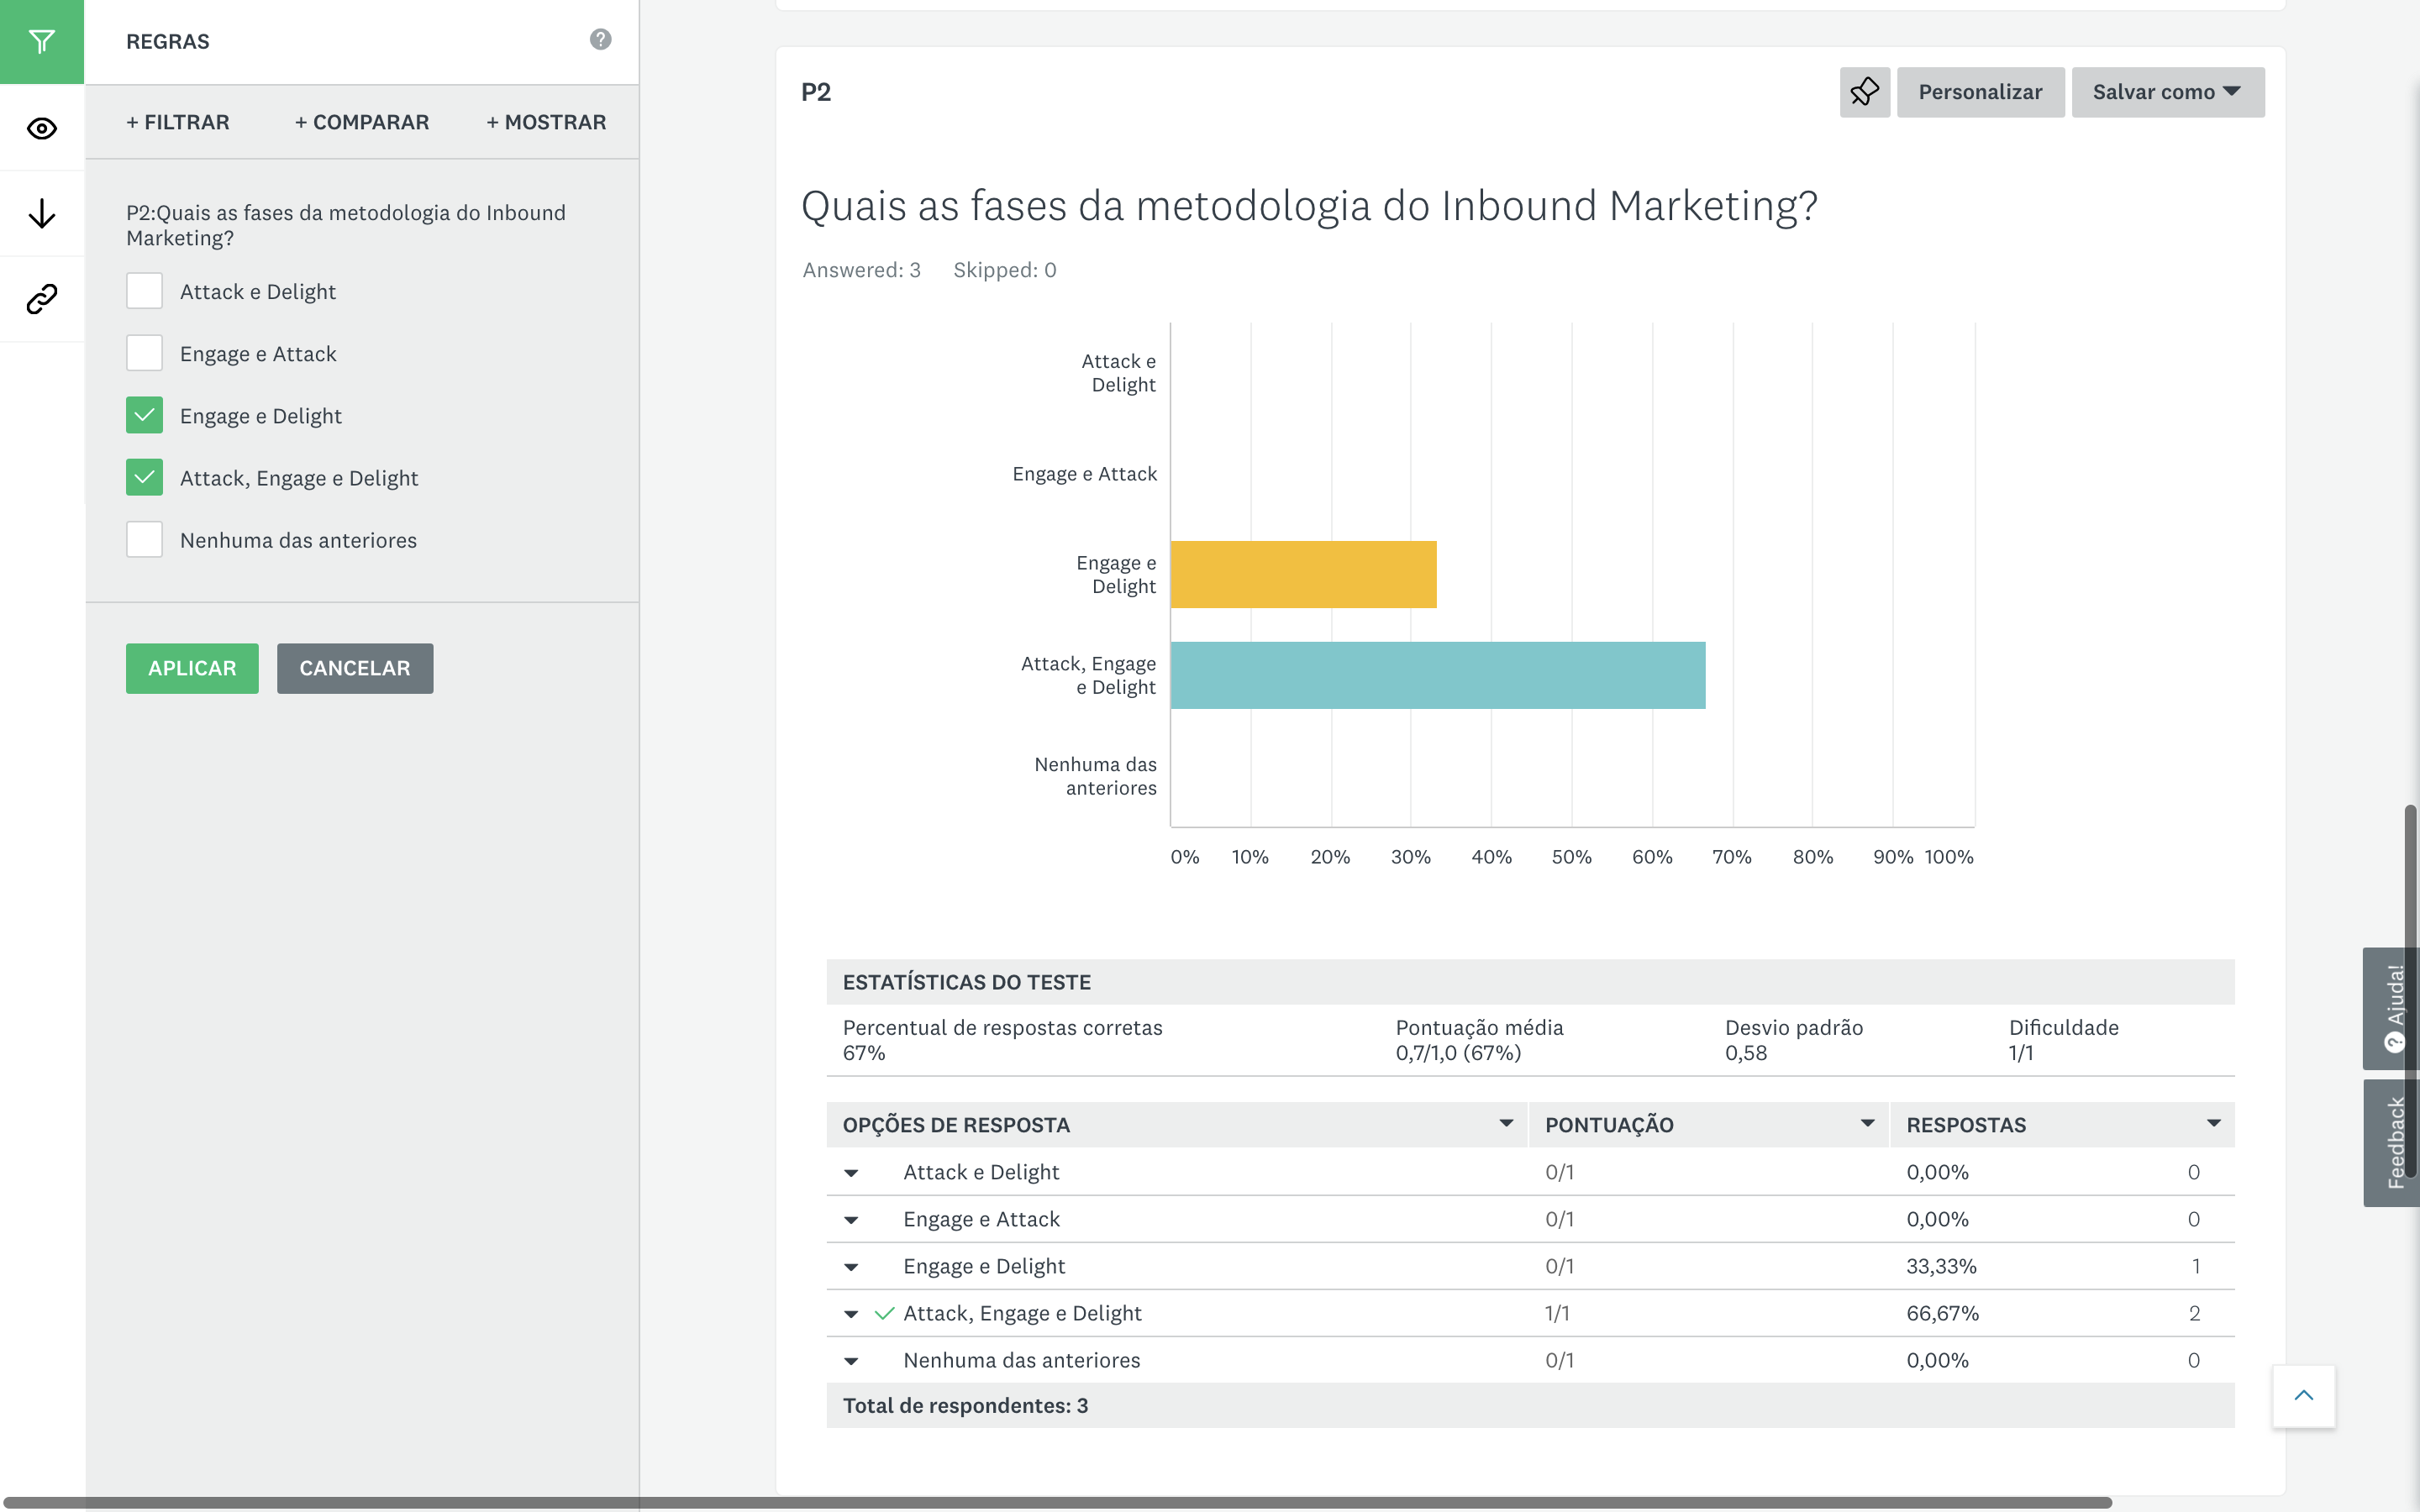
\includegraphics[width=1\textwidth]{img/sm/surveymonkey-form-filtro1}
		\caption{SurveyMonkey - Filtro aplicado na pergunta 2 }
		\label{fig:surveymonkey-form-filtro1}
	\end{center}
\end{figure}

\newpage



Para finalizar a plataforma SurveyMonkey tem ainda uma funcionalidade que, através da representação dos dados numa linha temporal, permite o utilizador perceber as tendências dos dados.

\section{Typeform}
\label{typeform}

O Typeform é uma plataforma \acrshort{saas} de criação de formulários online. É uma empresa que afirma resolver o problema dos formulários e inquéritos aborrecidos e tem também como proposta de valor o facto de conseguir criar formulários e inquéritos sem ter que programar uma única linhad e código. Esta plataforma permite recolher informações do público alvo através de formulários e inquéritos personalizados e no final visualizar estes dados. 

O Typeform disponilibilisa um pacote gratuito, contudo, é necessário criar conta de utilizador, para aceder ás funcionalidades da plataforma. Tanto o registro como o início de sessão pode ser feito através da \acrfull{api} do Google.

Como podemos ver na Figura \ref{fig:tf-dashboard}, no painel de controlo, podemos criar várias áreas de trabalho. Cada área de trabalho é independente e todos os formulários e inquéritos que forem adicionados ao mesmo podem ser partilhados com mais do que uma pessoa.
\newpage

\begin{figure}[ht!]
	\begin{center}
		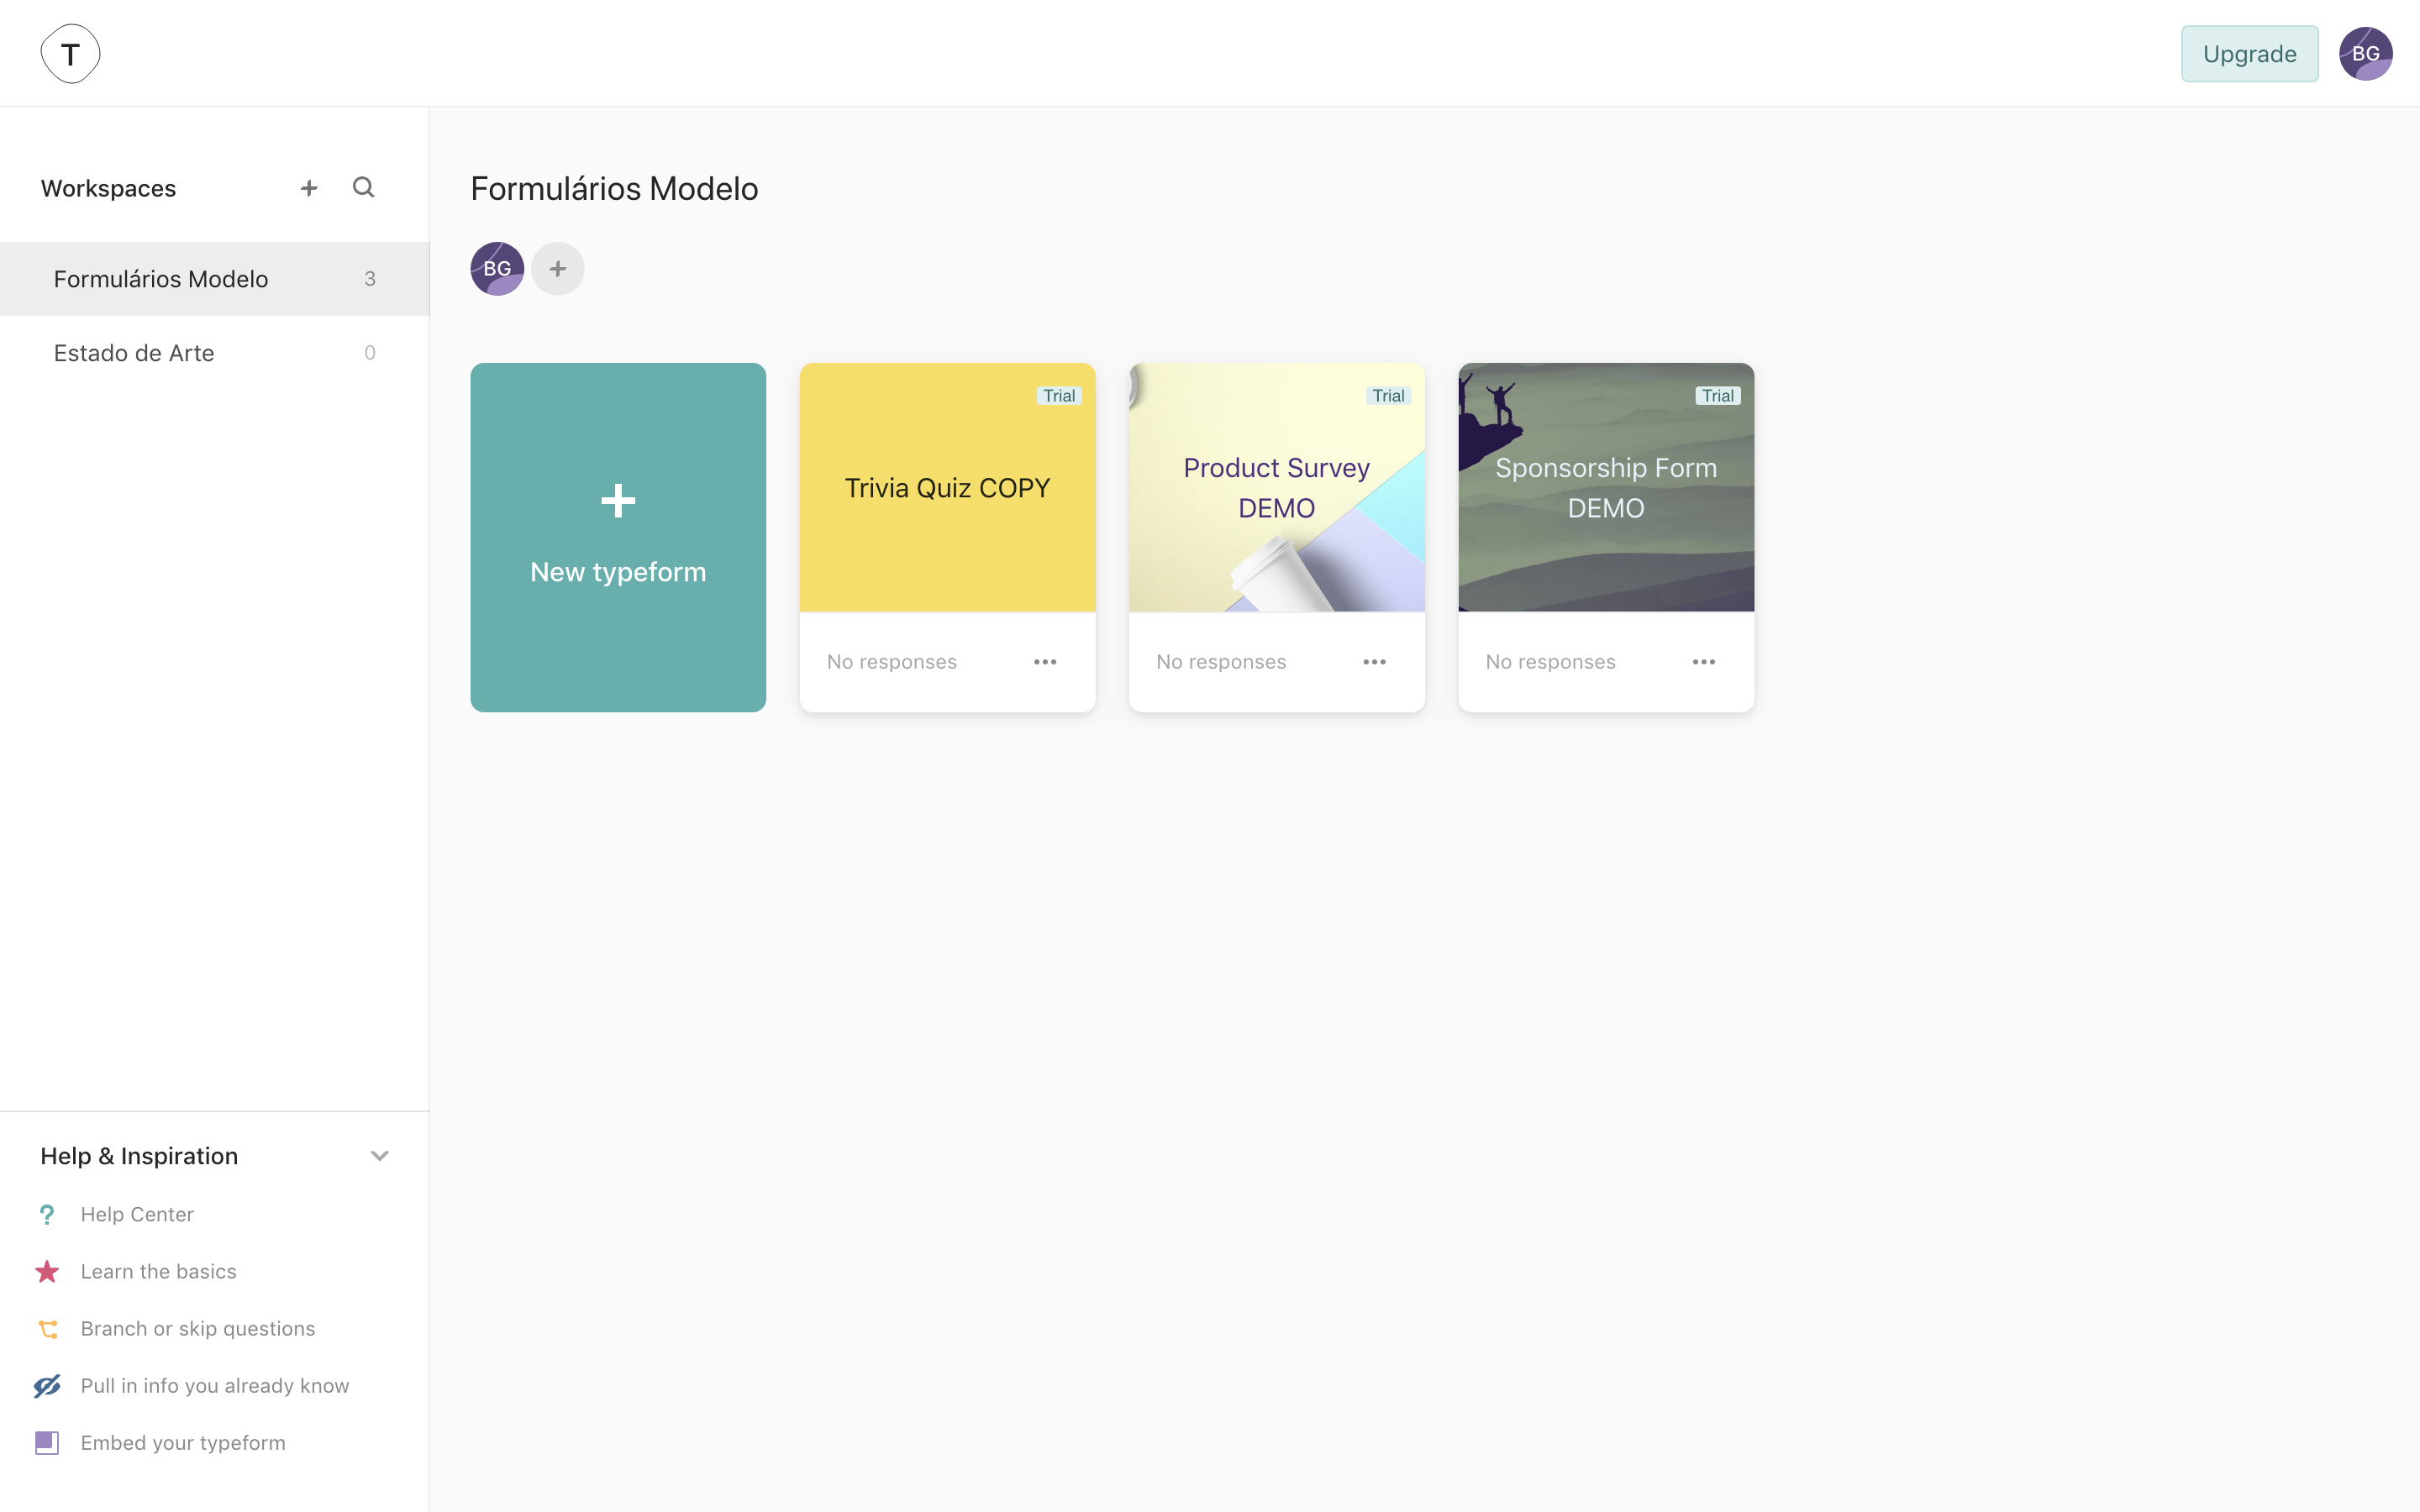
\includegraphics[width=1\textwidth]{img/tf/tf-dashboard}
		\caption{Typeform - Painel de Controlo}
		\label{fig:tf-dashboard}
	\end{center}
\end{figure}

Na criação de um formulário ou inquérito, do zero, a plataforma lista uma séria de templates que se podem filtrar por categorias na coluna à esquerda, como se pode observar na Figura \ref{fig:tf-form-create}.

\begin{figure}[ht!]
	\begin{center}
		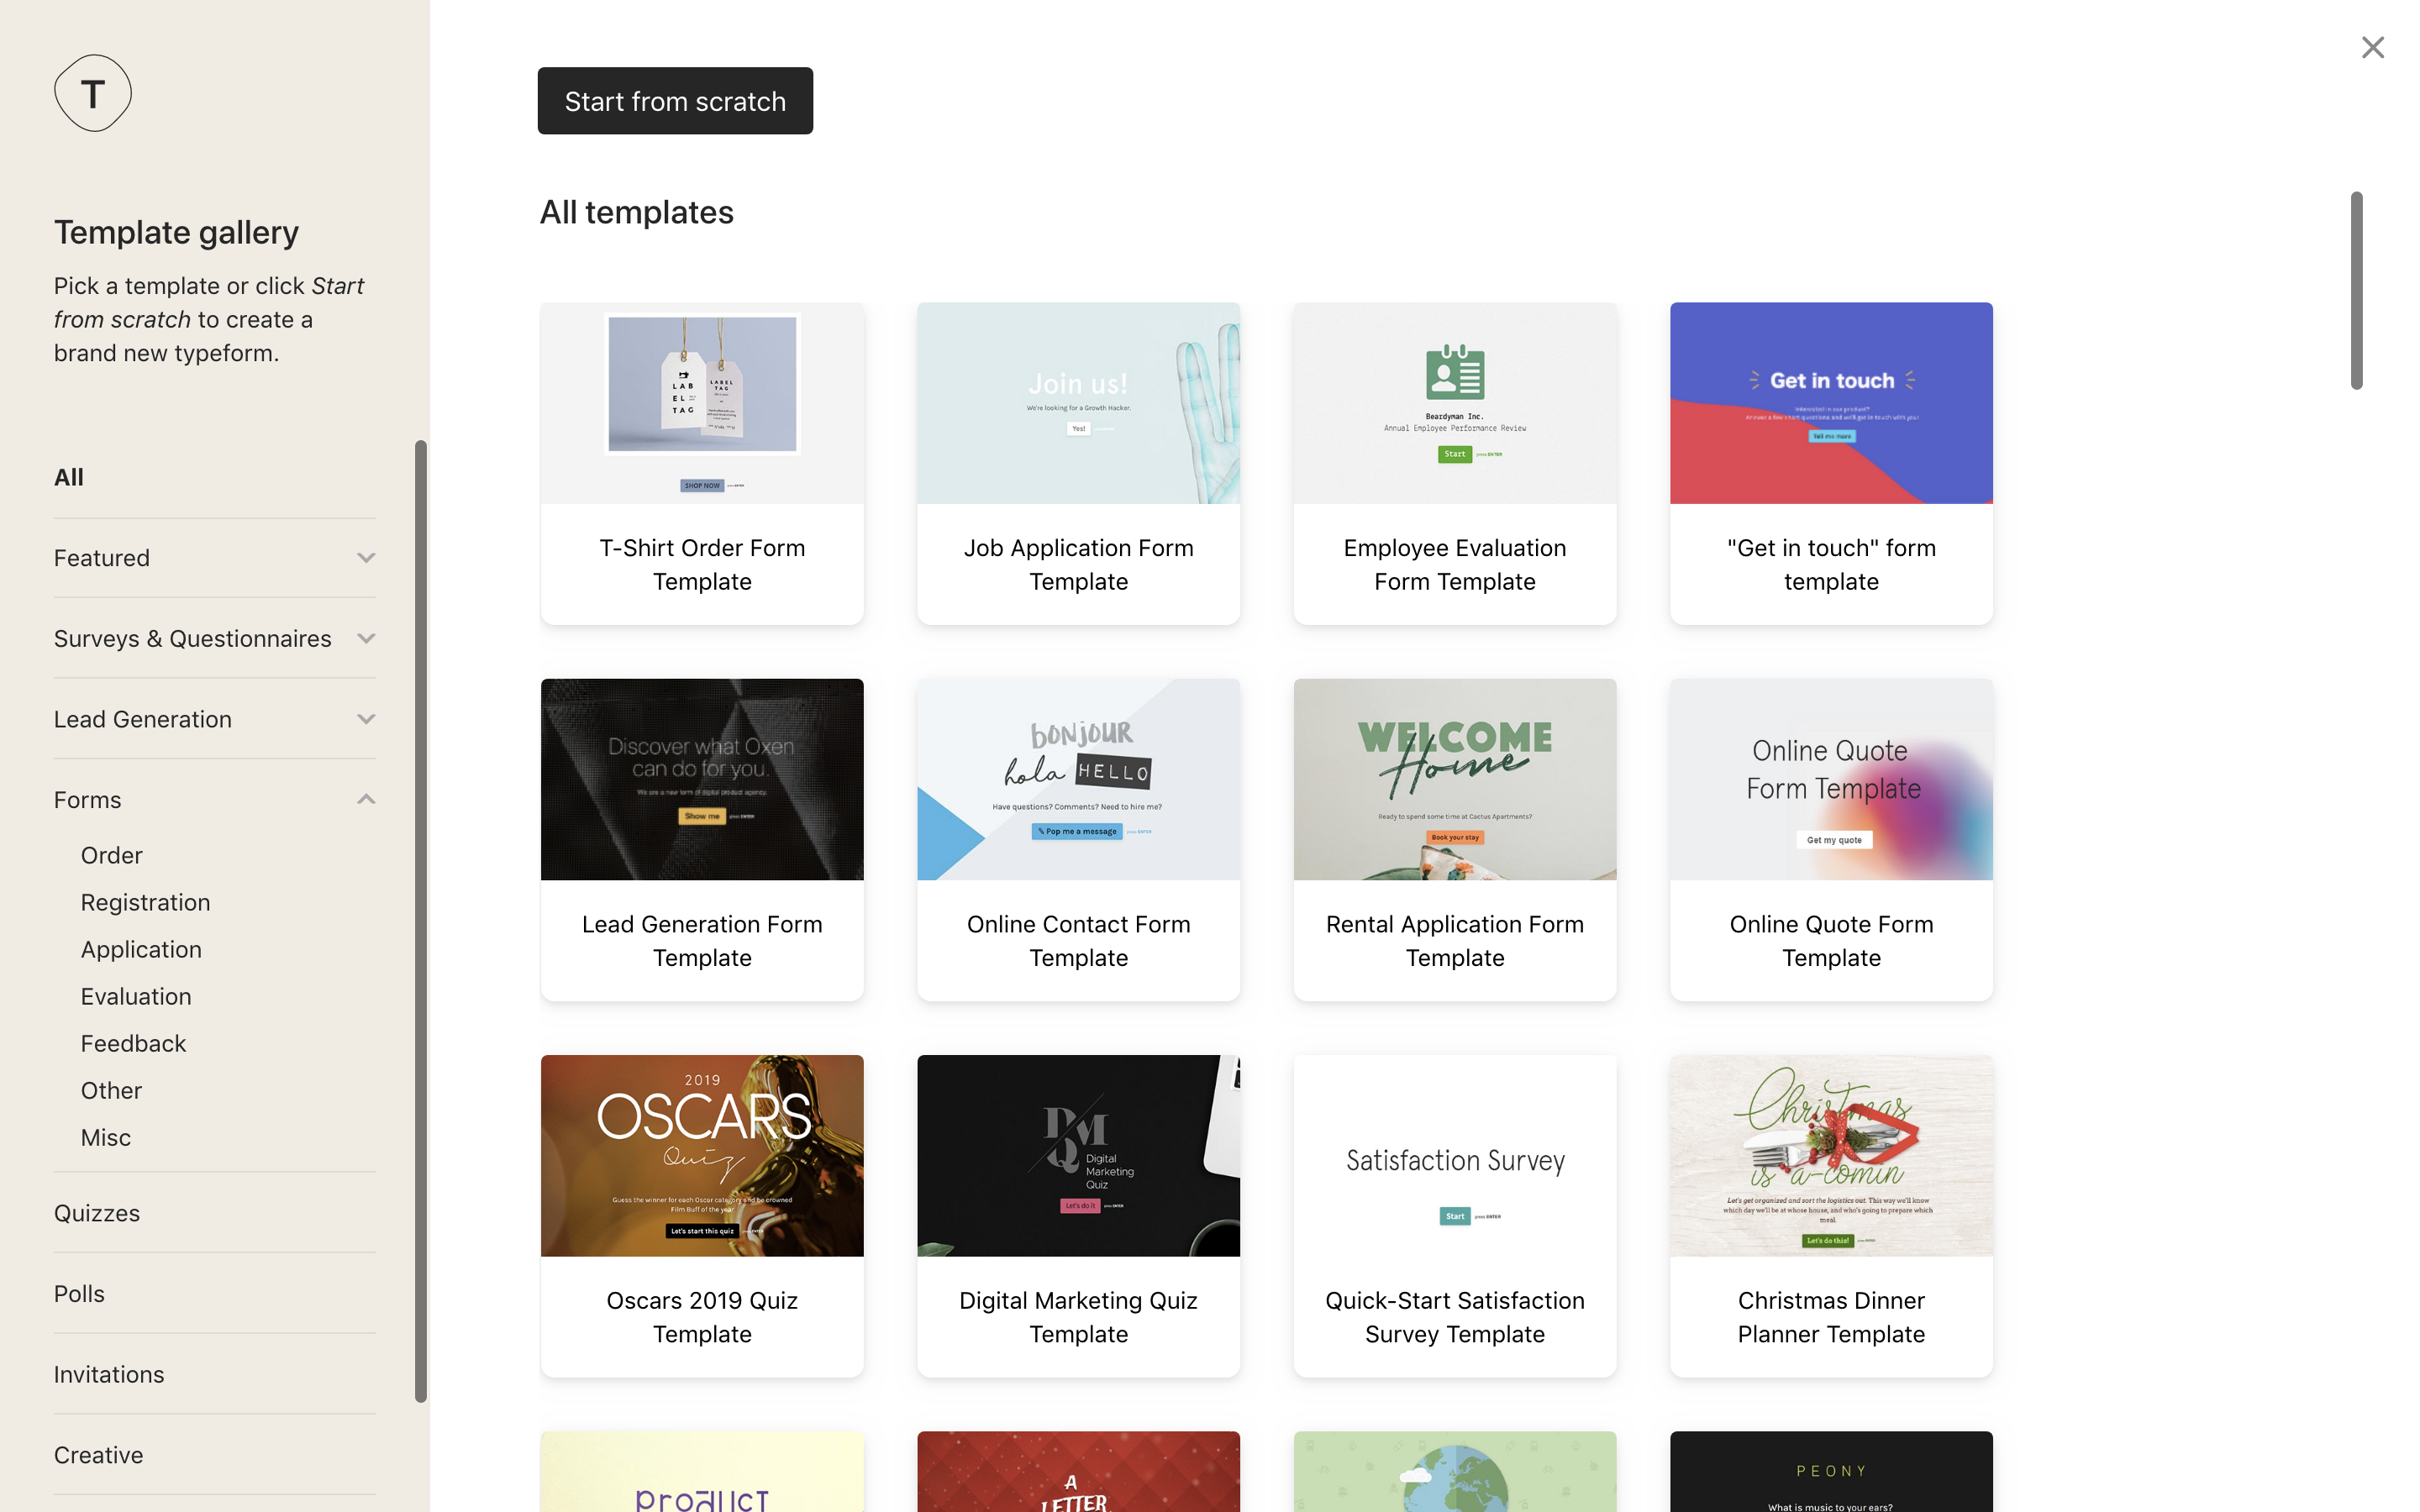
\includegraphics[width=1\textwidth]{img/tf/tf-form-create}
		\caption{Typeform - Criar Formulário}
		\label{fig:tf-form-create}
	\end{center}
\end{figure}
\newpage

\begin{figure}[ht!]
	\begin{center}
		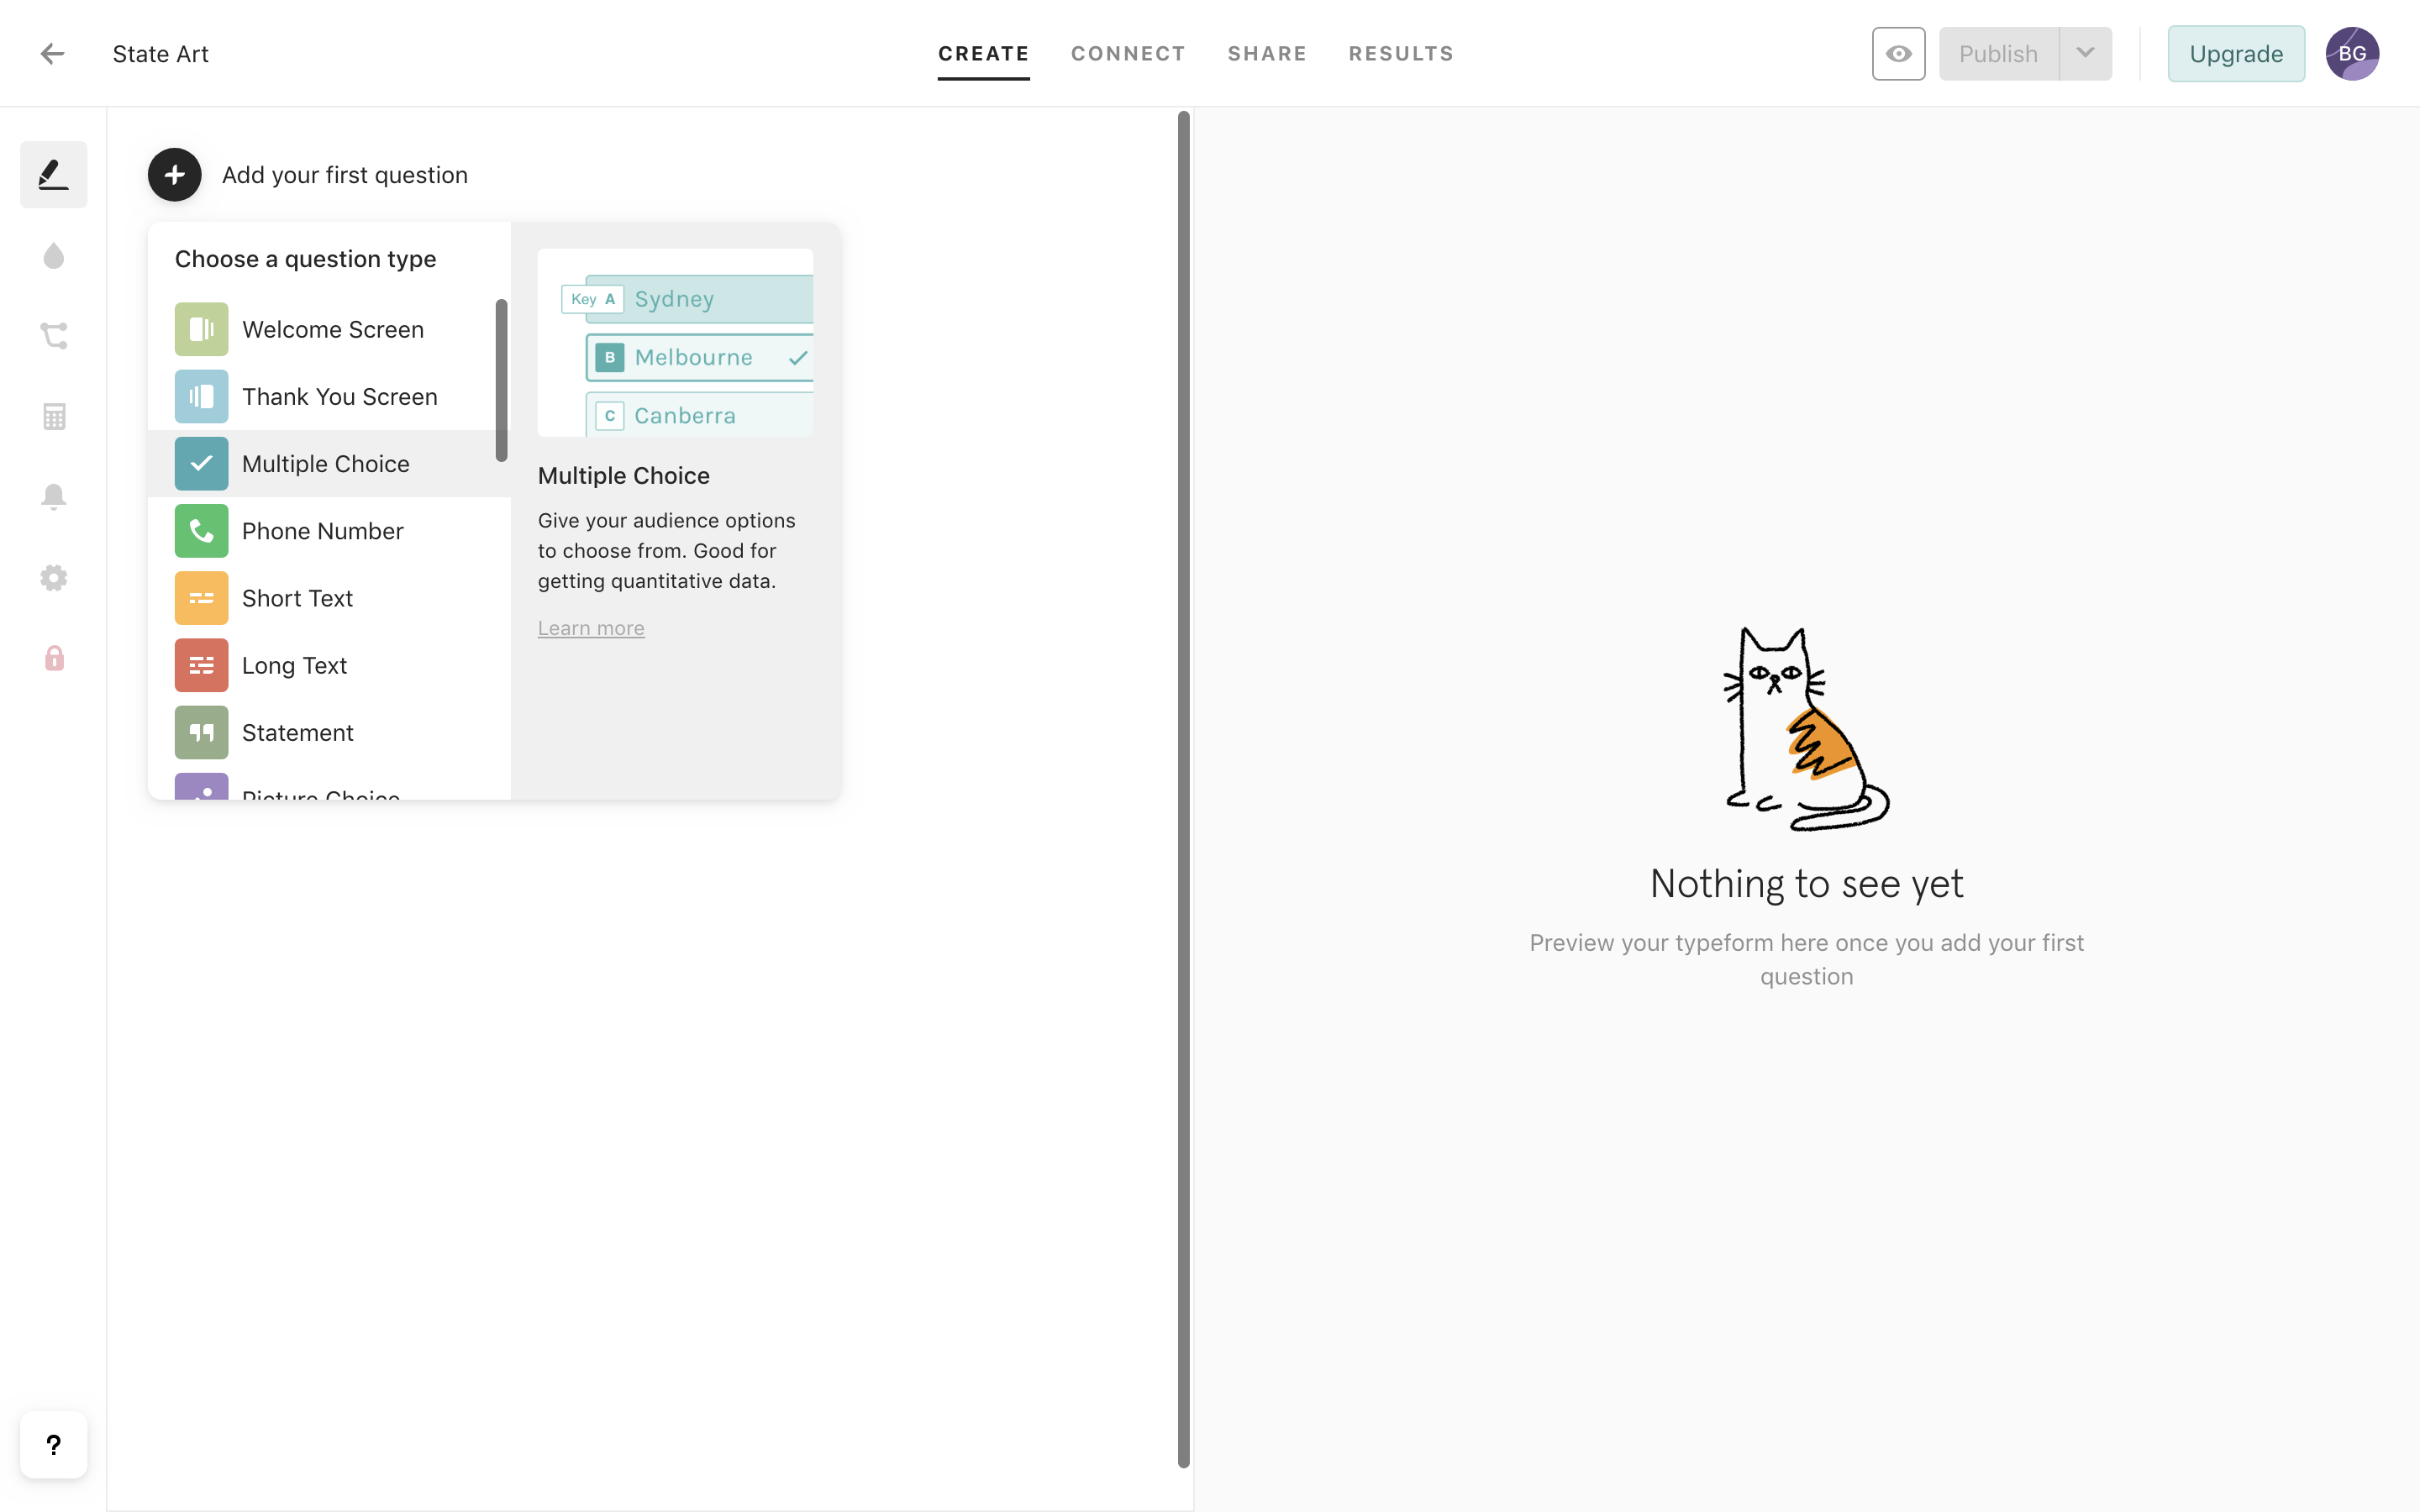
\includegraphics[width=1\textwidth]{img/tf/tf-question-type}
		\caption{Typeform - Tipos de pergunta}
		\label{fig:tf-question-type}
	\end{center}
\end{figure}

Representado na Figura \ref{fig:tf-question-type} temos os tipos de pergunta que a plataforma permite adicionar no formulário. Estas perguntas podem ser personalizaveis tanto a nível estético como funcional como podemos ver nas Figuras \ref{fig:tf-question-opcoes} e \ref{fig:tf-question-custom}, respectivamente. É também possível criar um tema novo para cada pergunta onde se pode escolher a fonte de texto, imagem de fundo e cores da pergunta, respostas, butões e fundo.

\begin{figure}[ht!]
	\begin{center}
		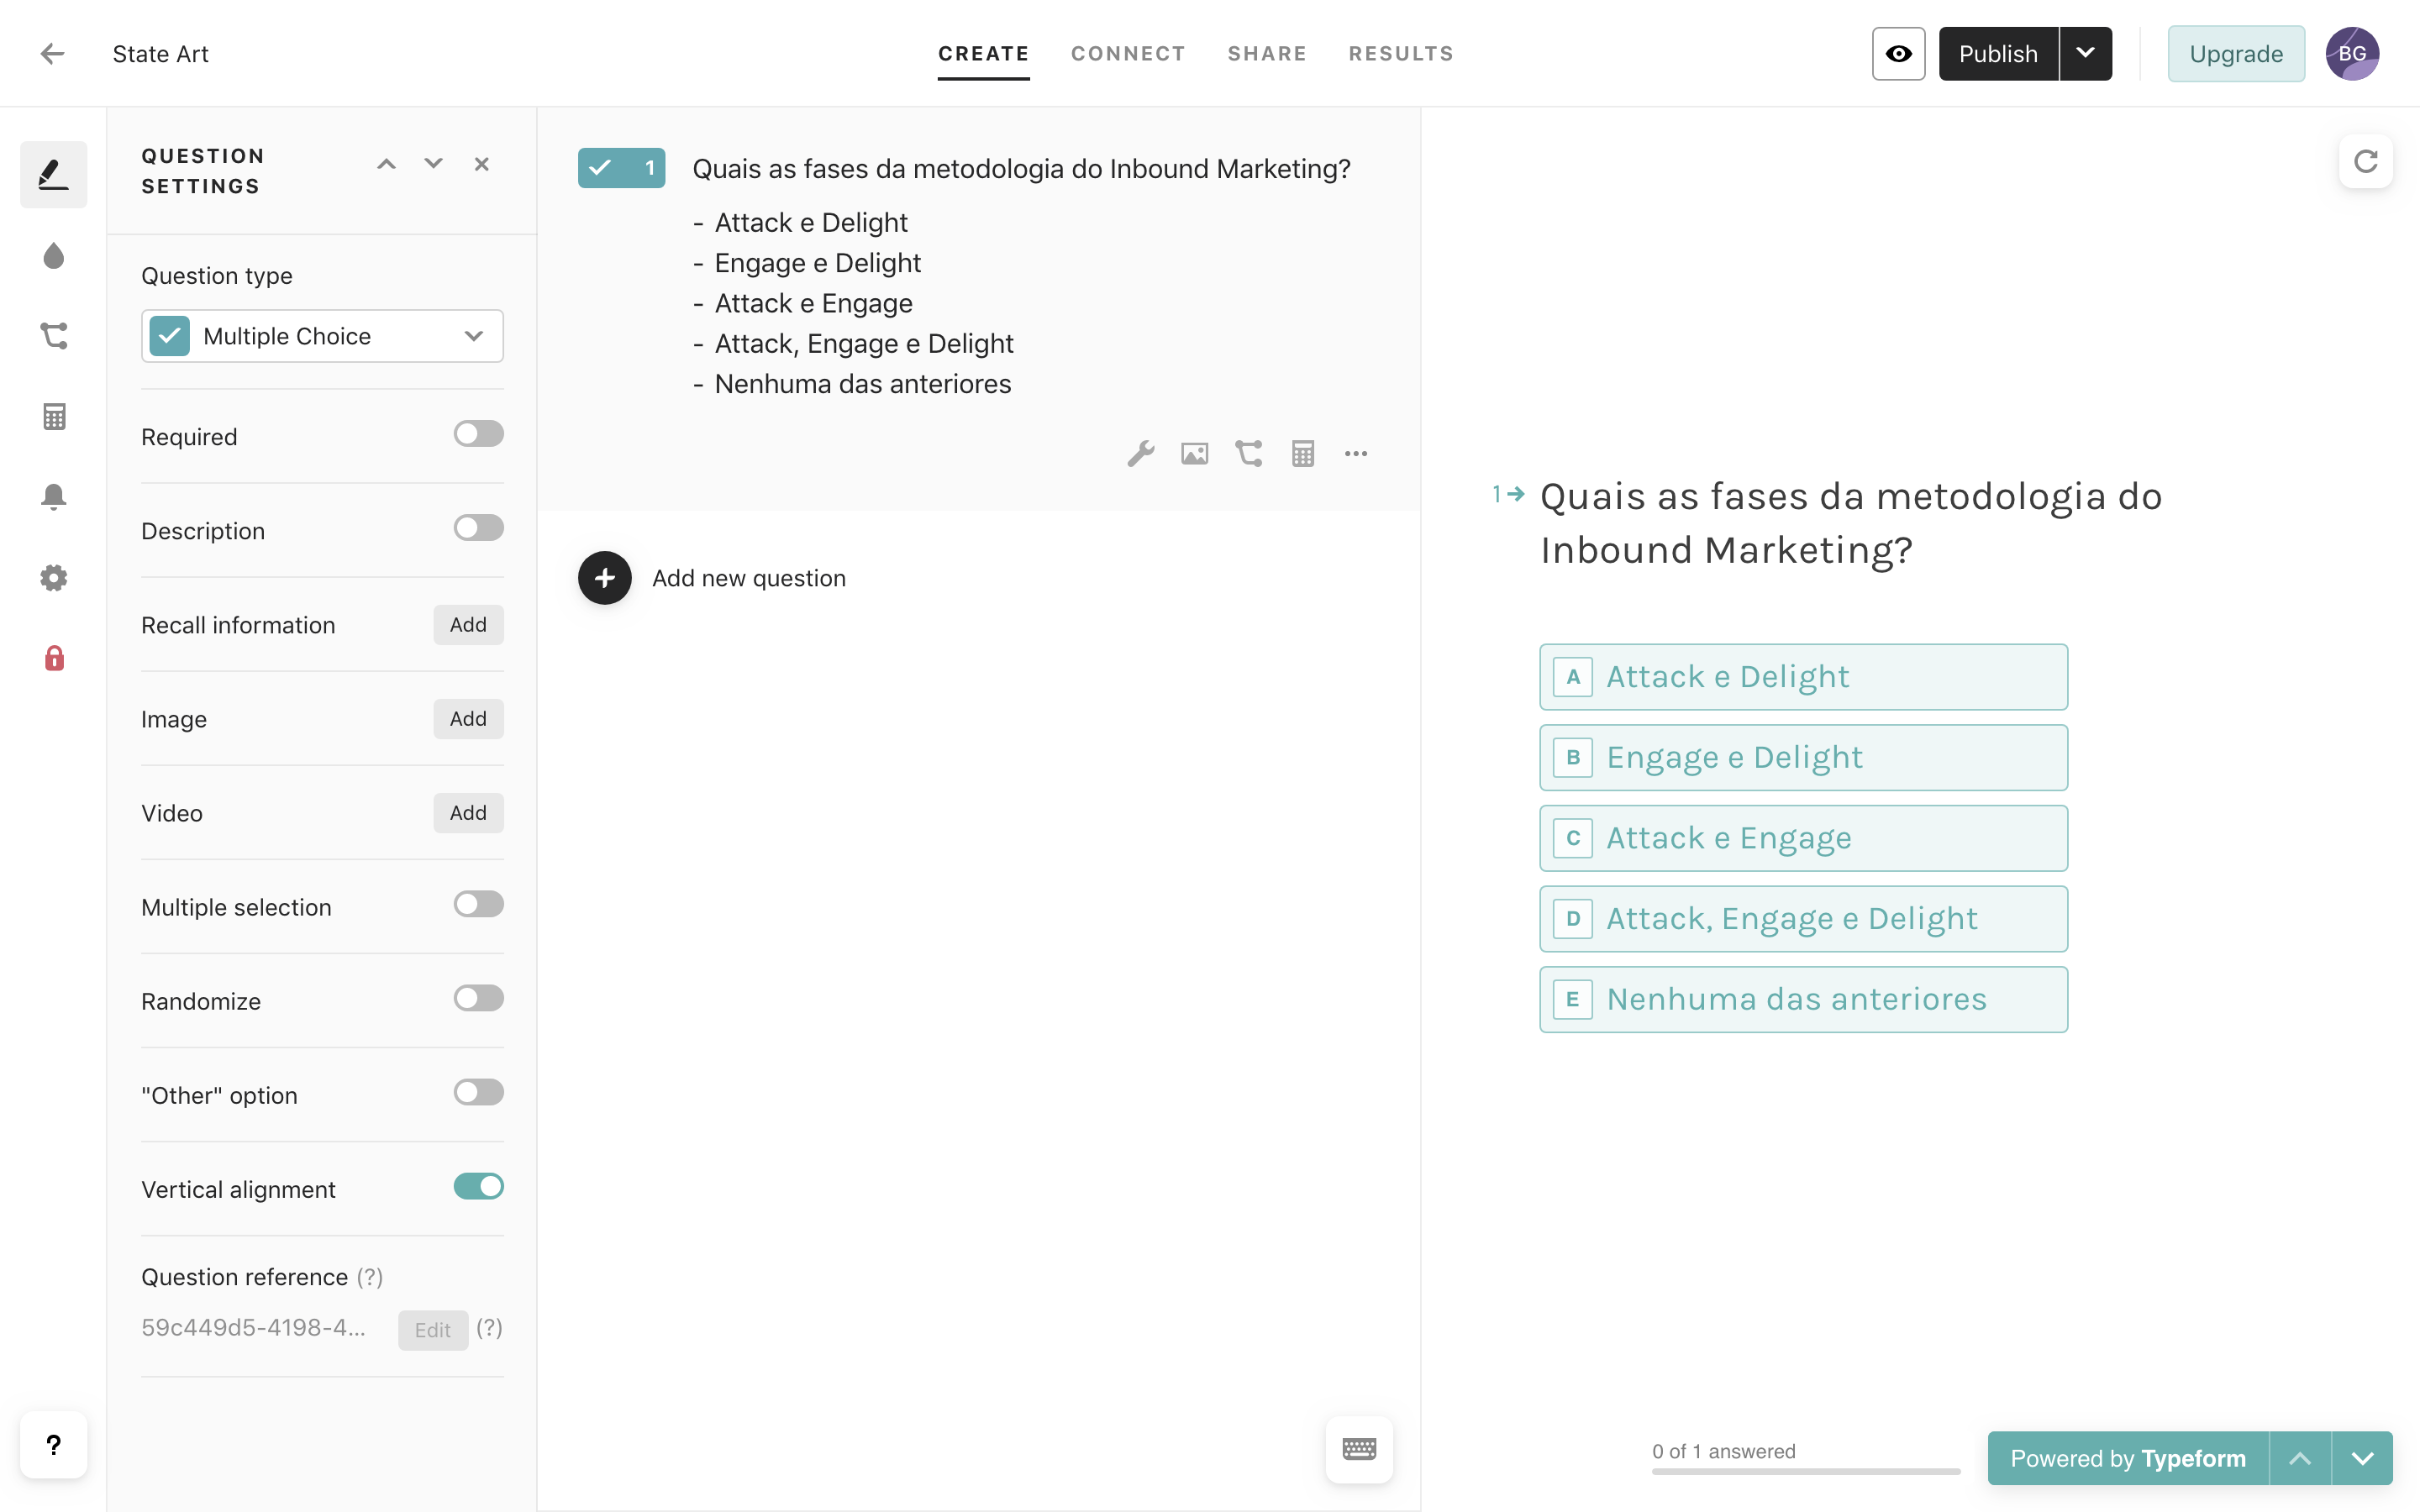
\includegraphics[width=1\textwidth]{img/tf/tf-question-opcoes}
		\caption{Typeform - Opções da pergunta}
		\label{fig:tf-question-opcoes}
	\end{center}
\end{figure}

\begin{figure}[ht!]
	\begin{center}
		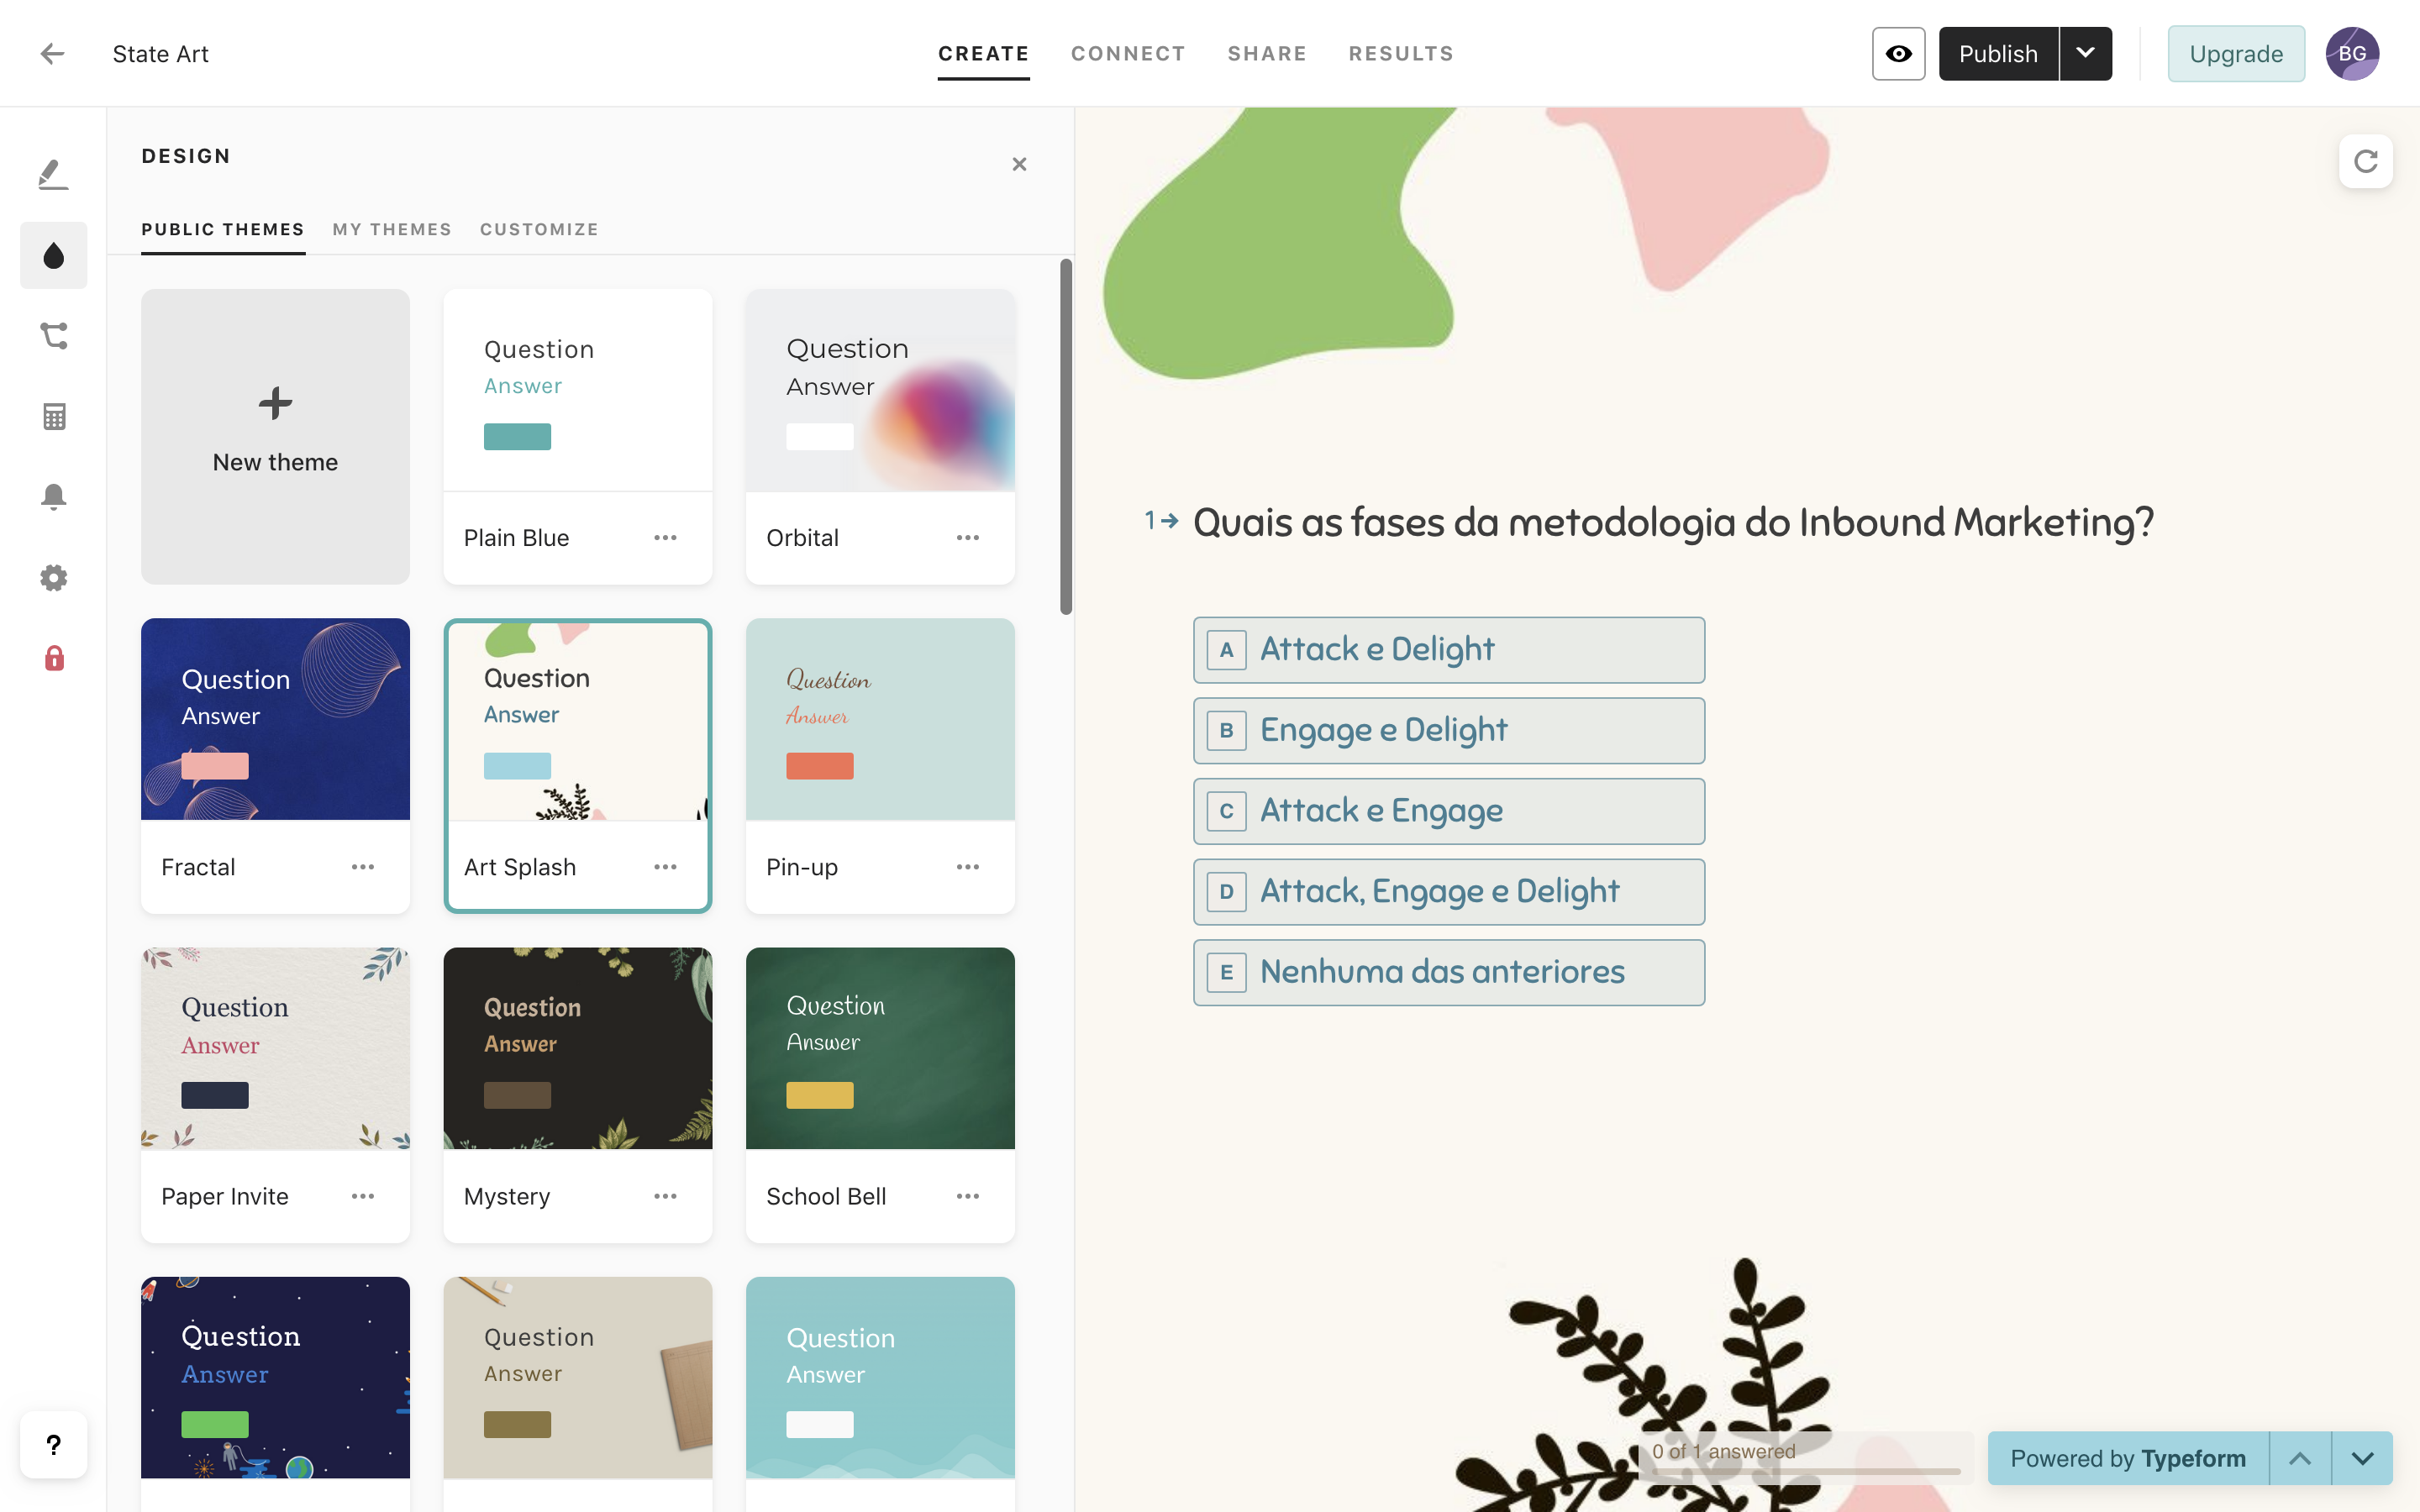
\includegraphics[width=1\textwidth]{img/tf/tf-question-custom}
		\caption{Typeform - Design da pergunta}
		\label{fig:tf-question-custom}
	\end{center}
\end{figure}
 
 A plataforma permite ainda os utilizadores adicionarem lógicas aos seus formulário, como exemplificado na Figura \ref{fig:tf-question-logica} , em que caso a resposta à pergunta 4 seja a especificada, o caminho a tomar será diferente. 
 

 
 \begin{figure}[ht!]
 	\begin{center}
 		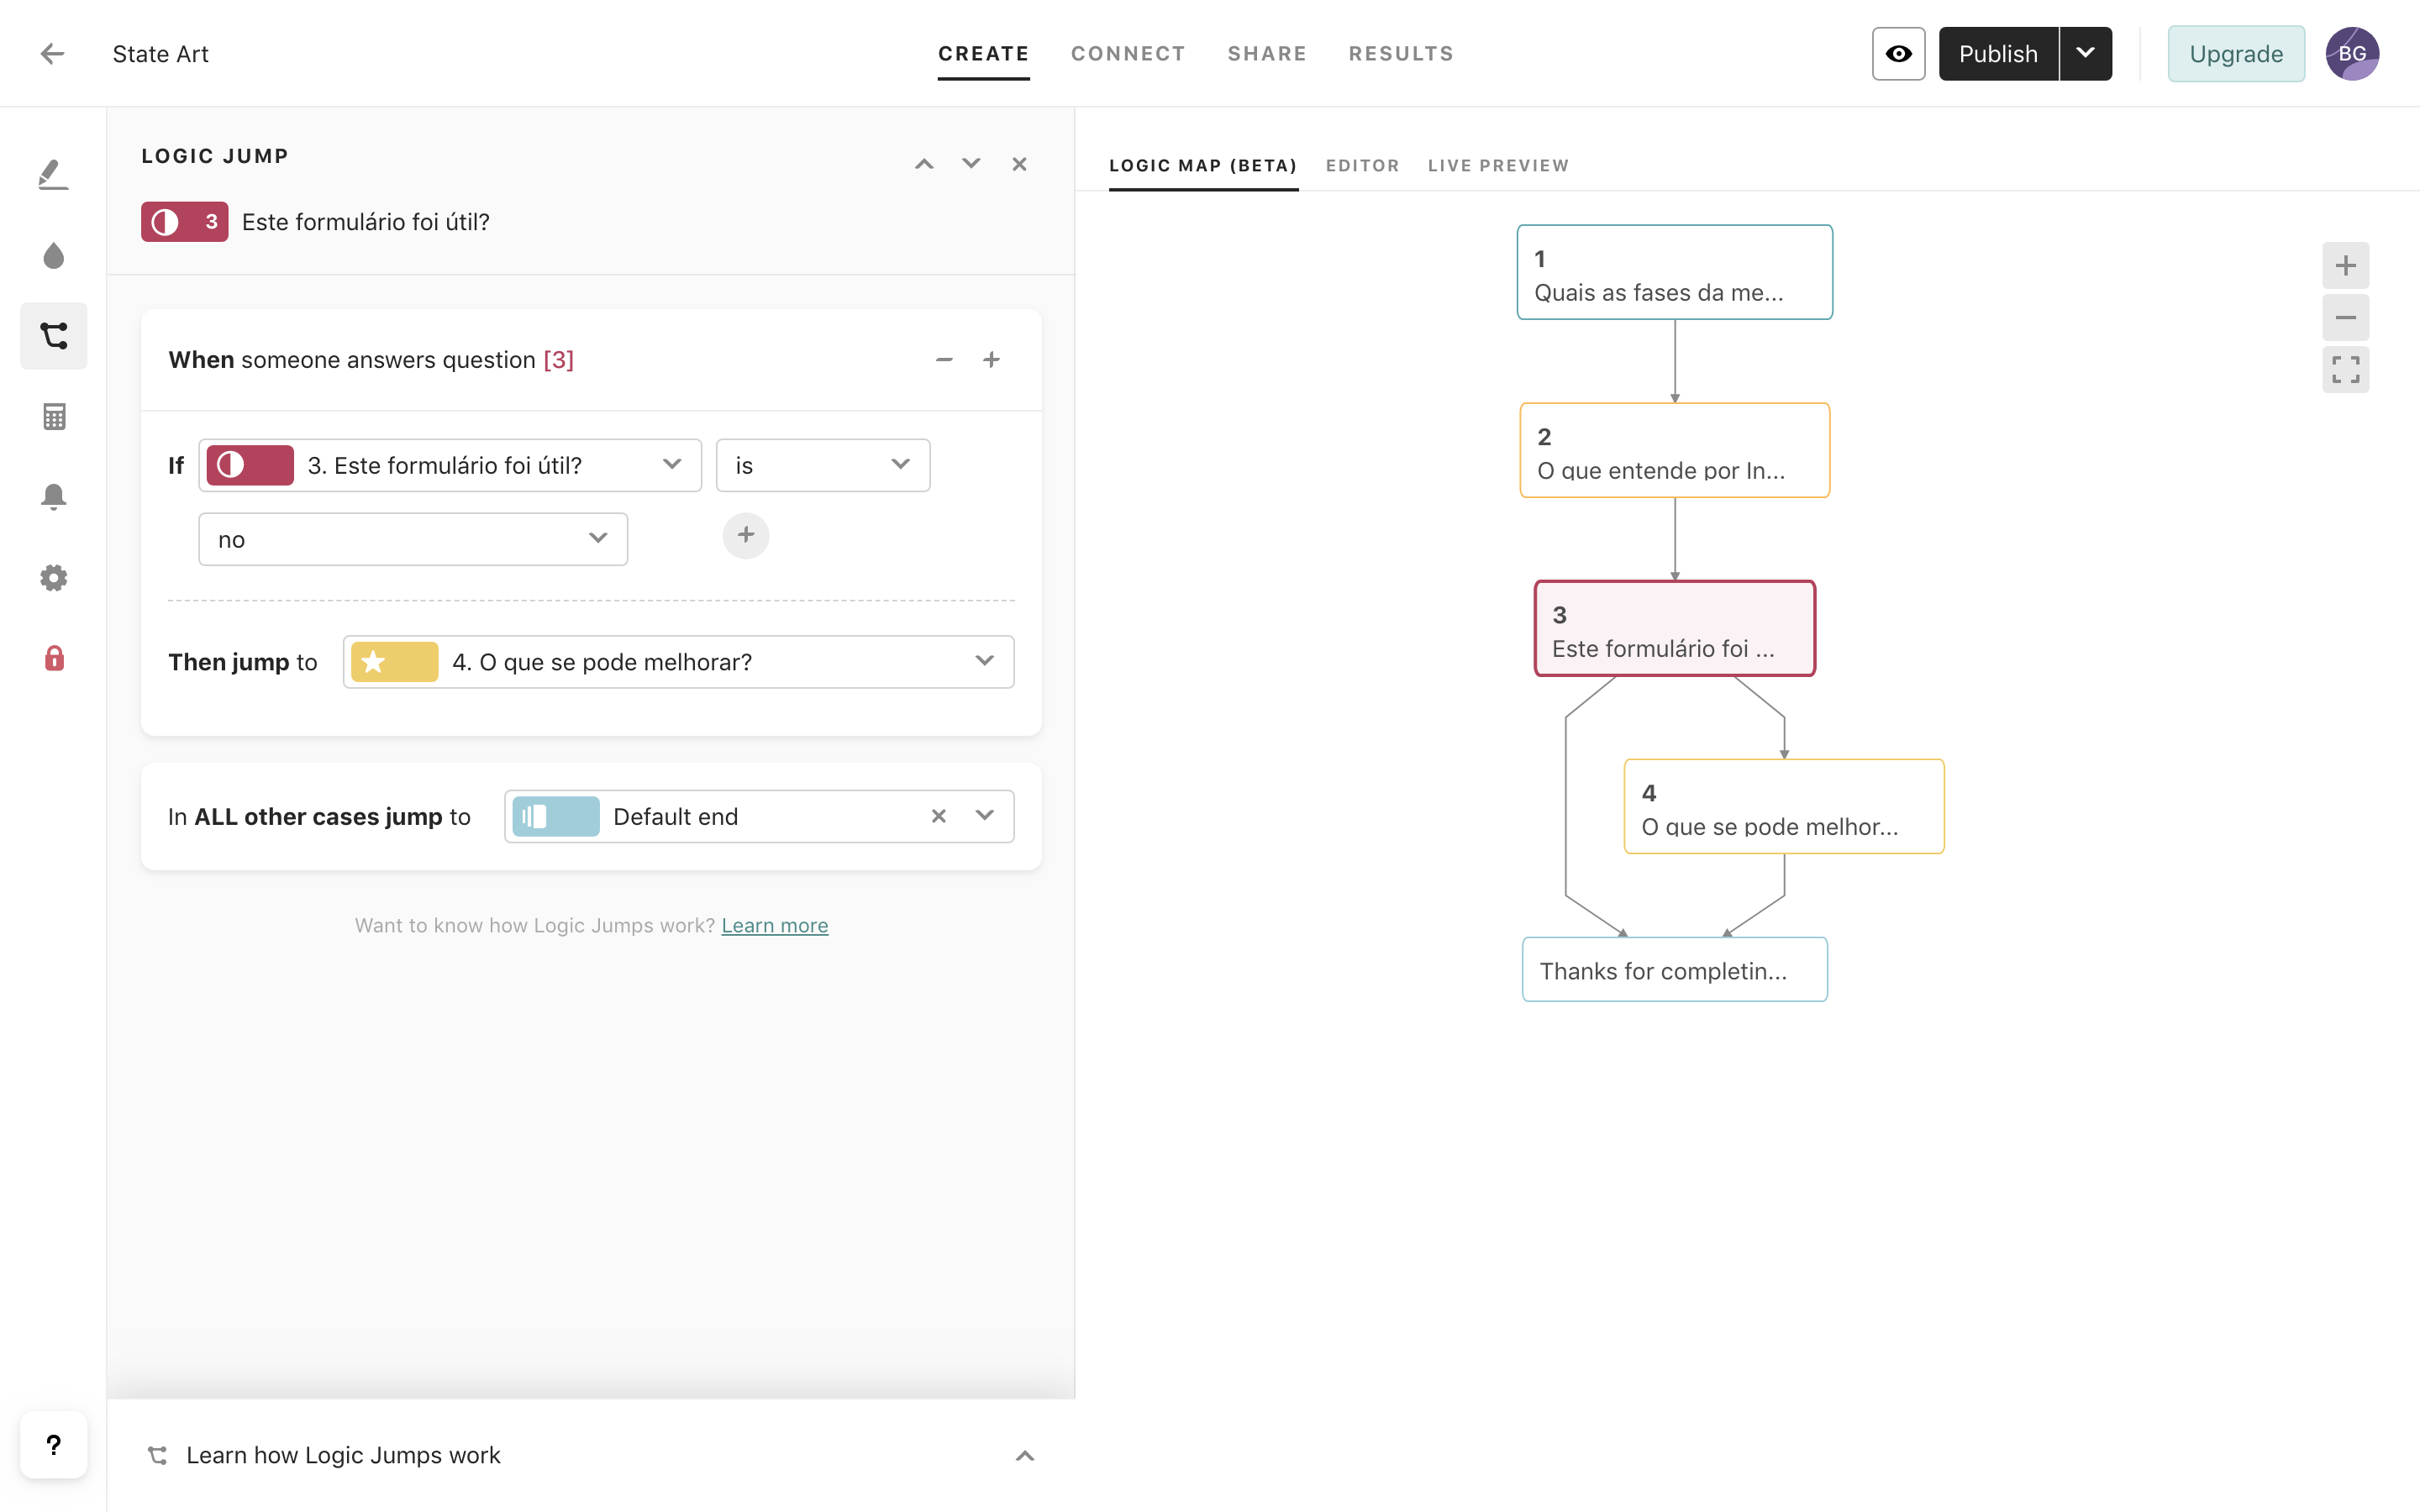
\includegraphics[width=1\textwidth]{img/tf/tf-question-logica}
 		\caption{Typeform - Lógica do formulário}
 		\label{fig:tf-question-logica}
 	\end{center}
 \end{figure}

\newpage

 A funcionalidade de visualizar o formulário está disponivel no canto superior direito, no lado esquerdo do botão de publicar, que permite o autor verificar se tudo está feito conforme planeado e assim poder publicar e partilhar.
 
 O Typeform permite também a integração de serviços externos com o formulário, como podemos ver na Figura \ref{fig:tf-question-integration} , em que, por exemplo, utilizando o Google Sheets\cite{googlesheets}, os resultados são exportados directamente para uma \textit{google sheet}


\begin{figure}[ht!]
	\begin{center}
		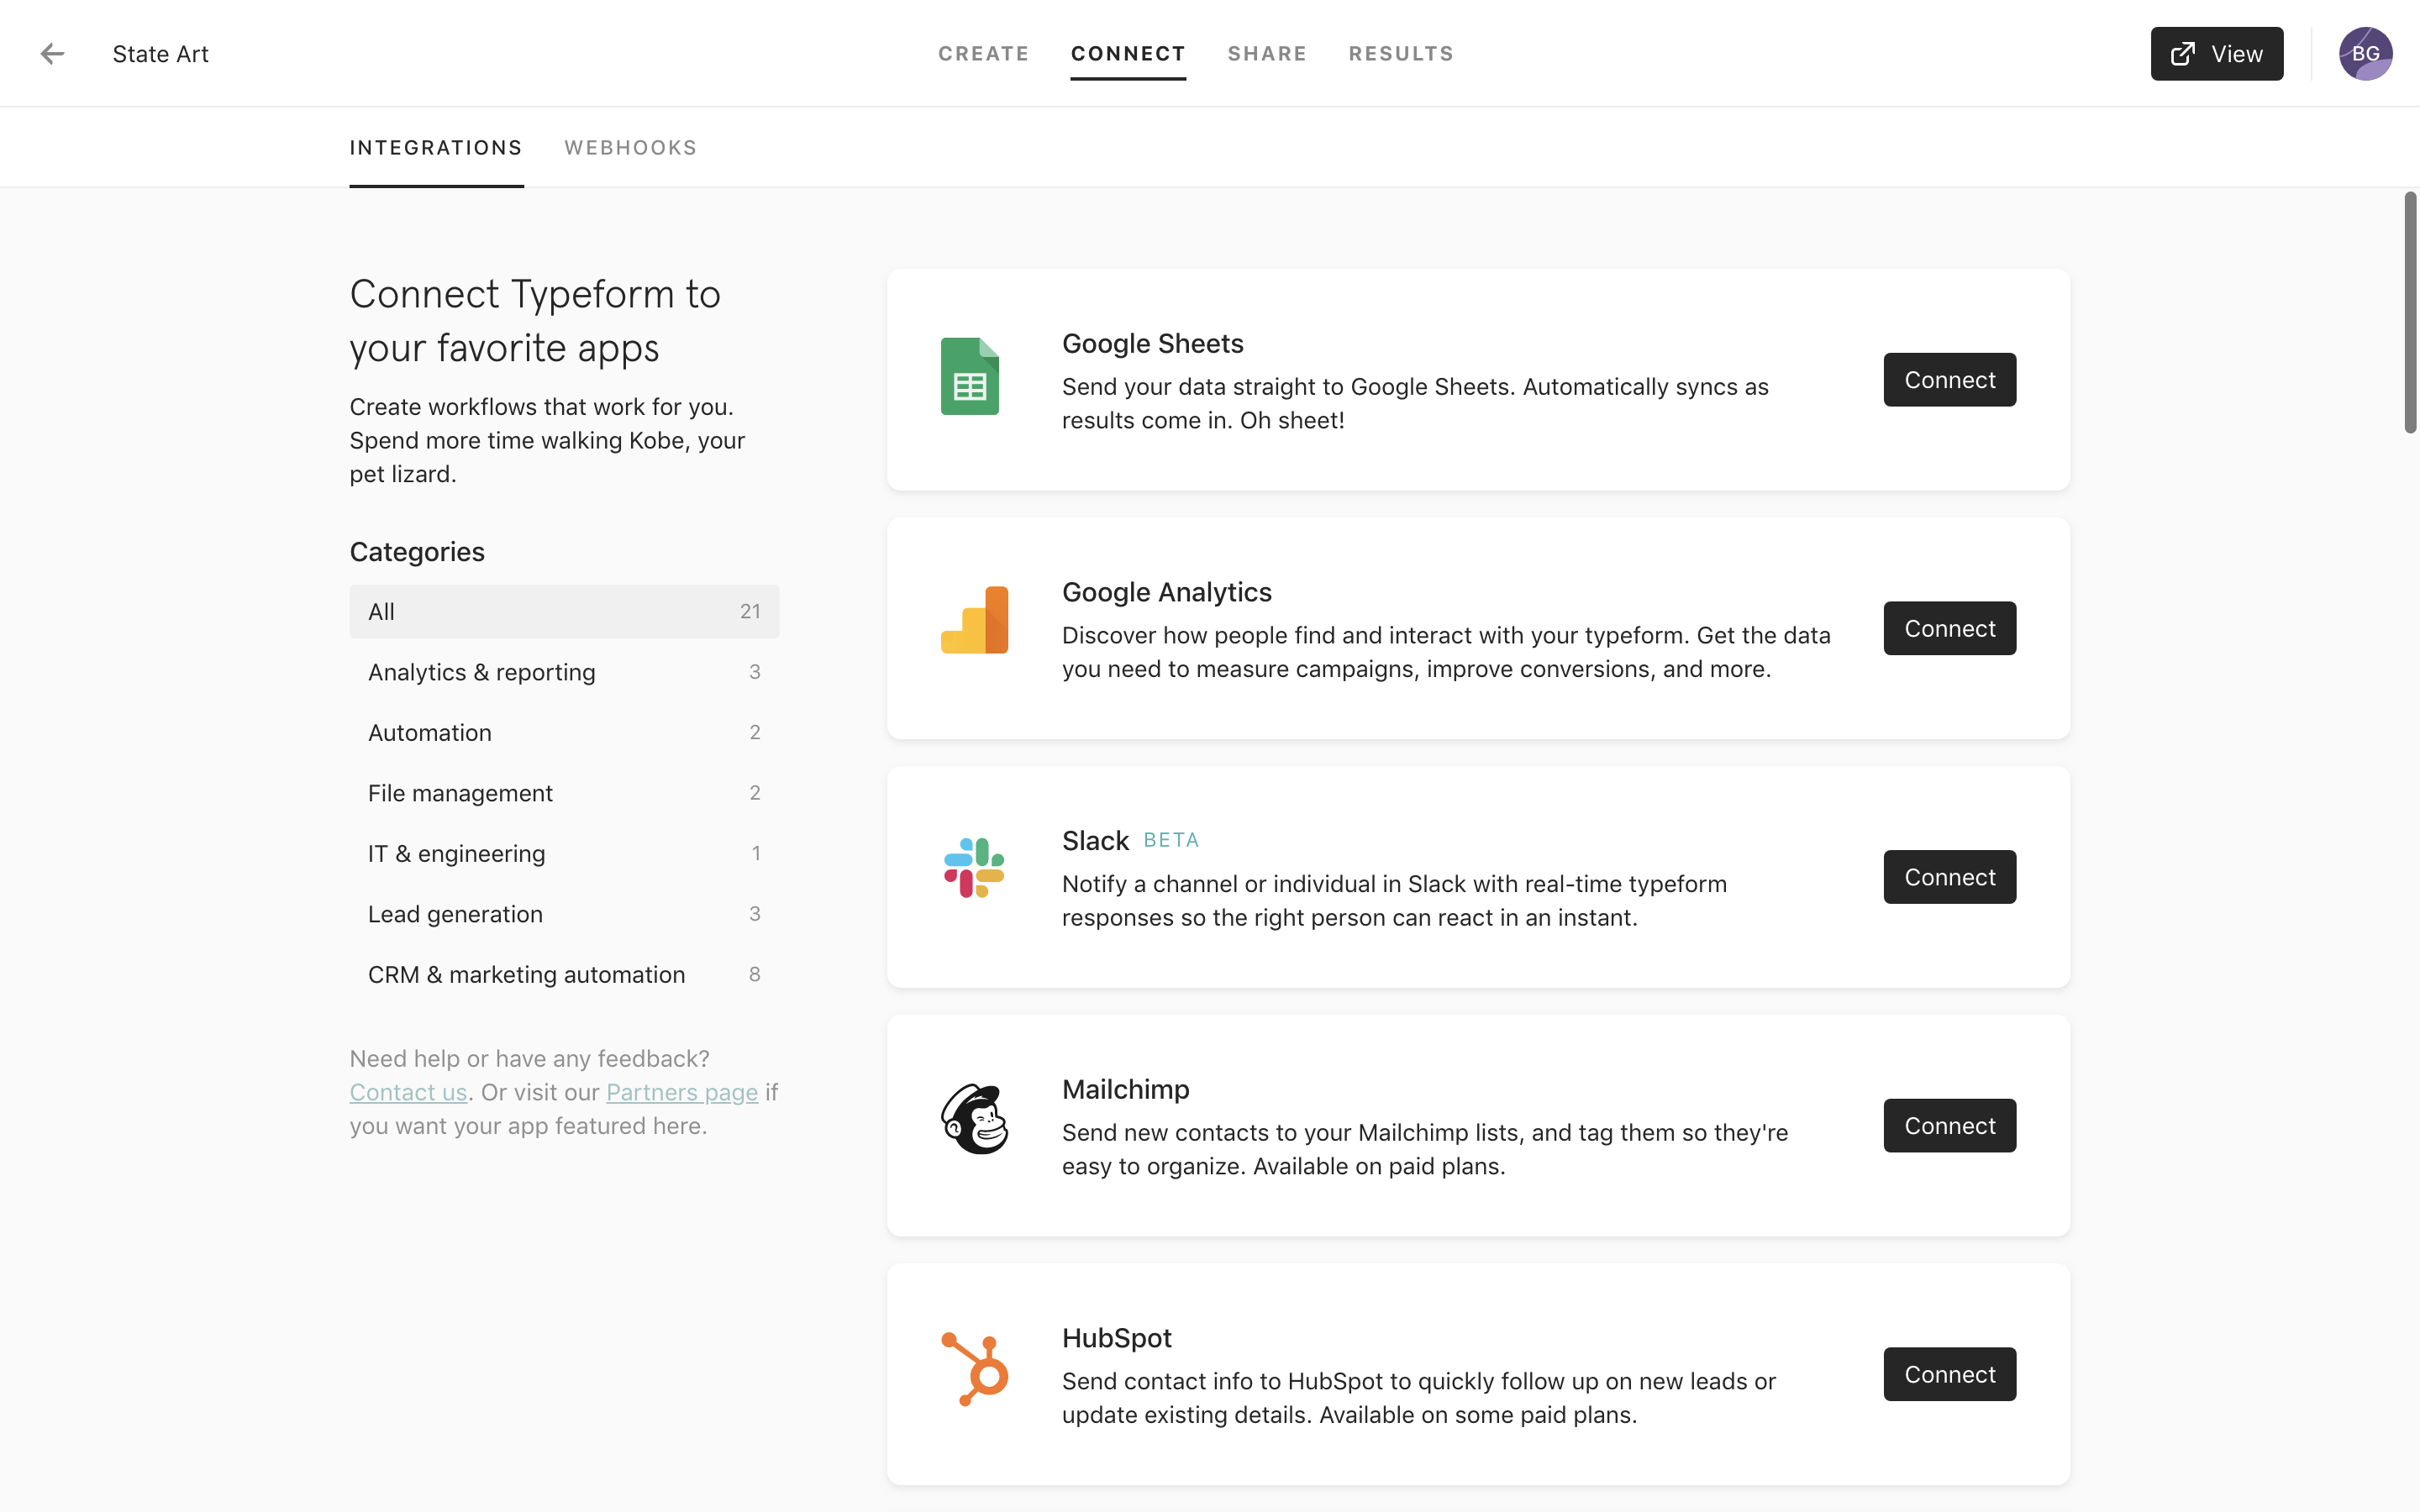
\includegraphics[width=1\textwidth]{img/tf/tf-question-integration}
		\caption{Typeform - Integração com sistemas externos}
		\label{fig:tf-question-integration}
	\end{center}
\end{figure}

Representado na Figura \ref{fig:tf-question-results} , temos a secção de analise de dados da plataforma onde podemos ver uma sumarização dos dados recebidos ou  analisar todas as respostas uma a uma. É também possível gerar um reportório dos dados recebidos e partilhar com alguém em qualquer fase, por exemplo, de uma campanha, uma vez que o mesmo é actualizado automaticamente com as novas respostas recebidas. 

O Typeform não fornece quaisquer filtros para segmentar os dados, contudo, fora as respostas em si, exibe algumas estatísticas/métricas relacionadas com os dispositivos que foram utilizados para responder aos formulários.


\newpage
\begin{figure}[ht!]
	\begin{center}
		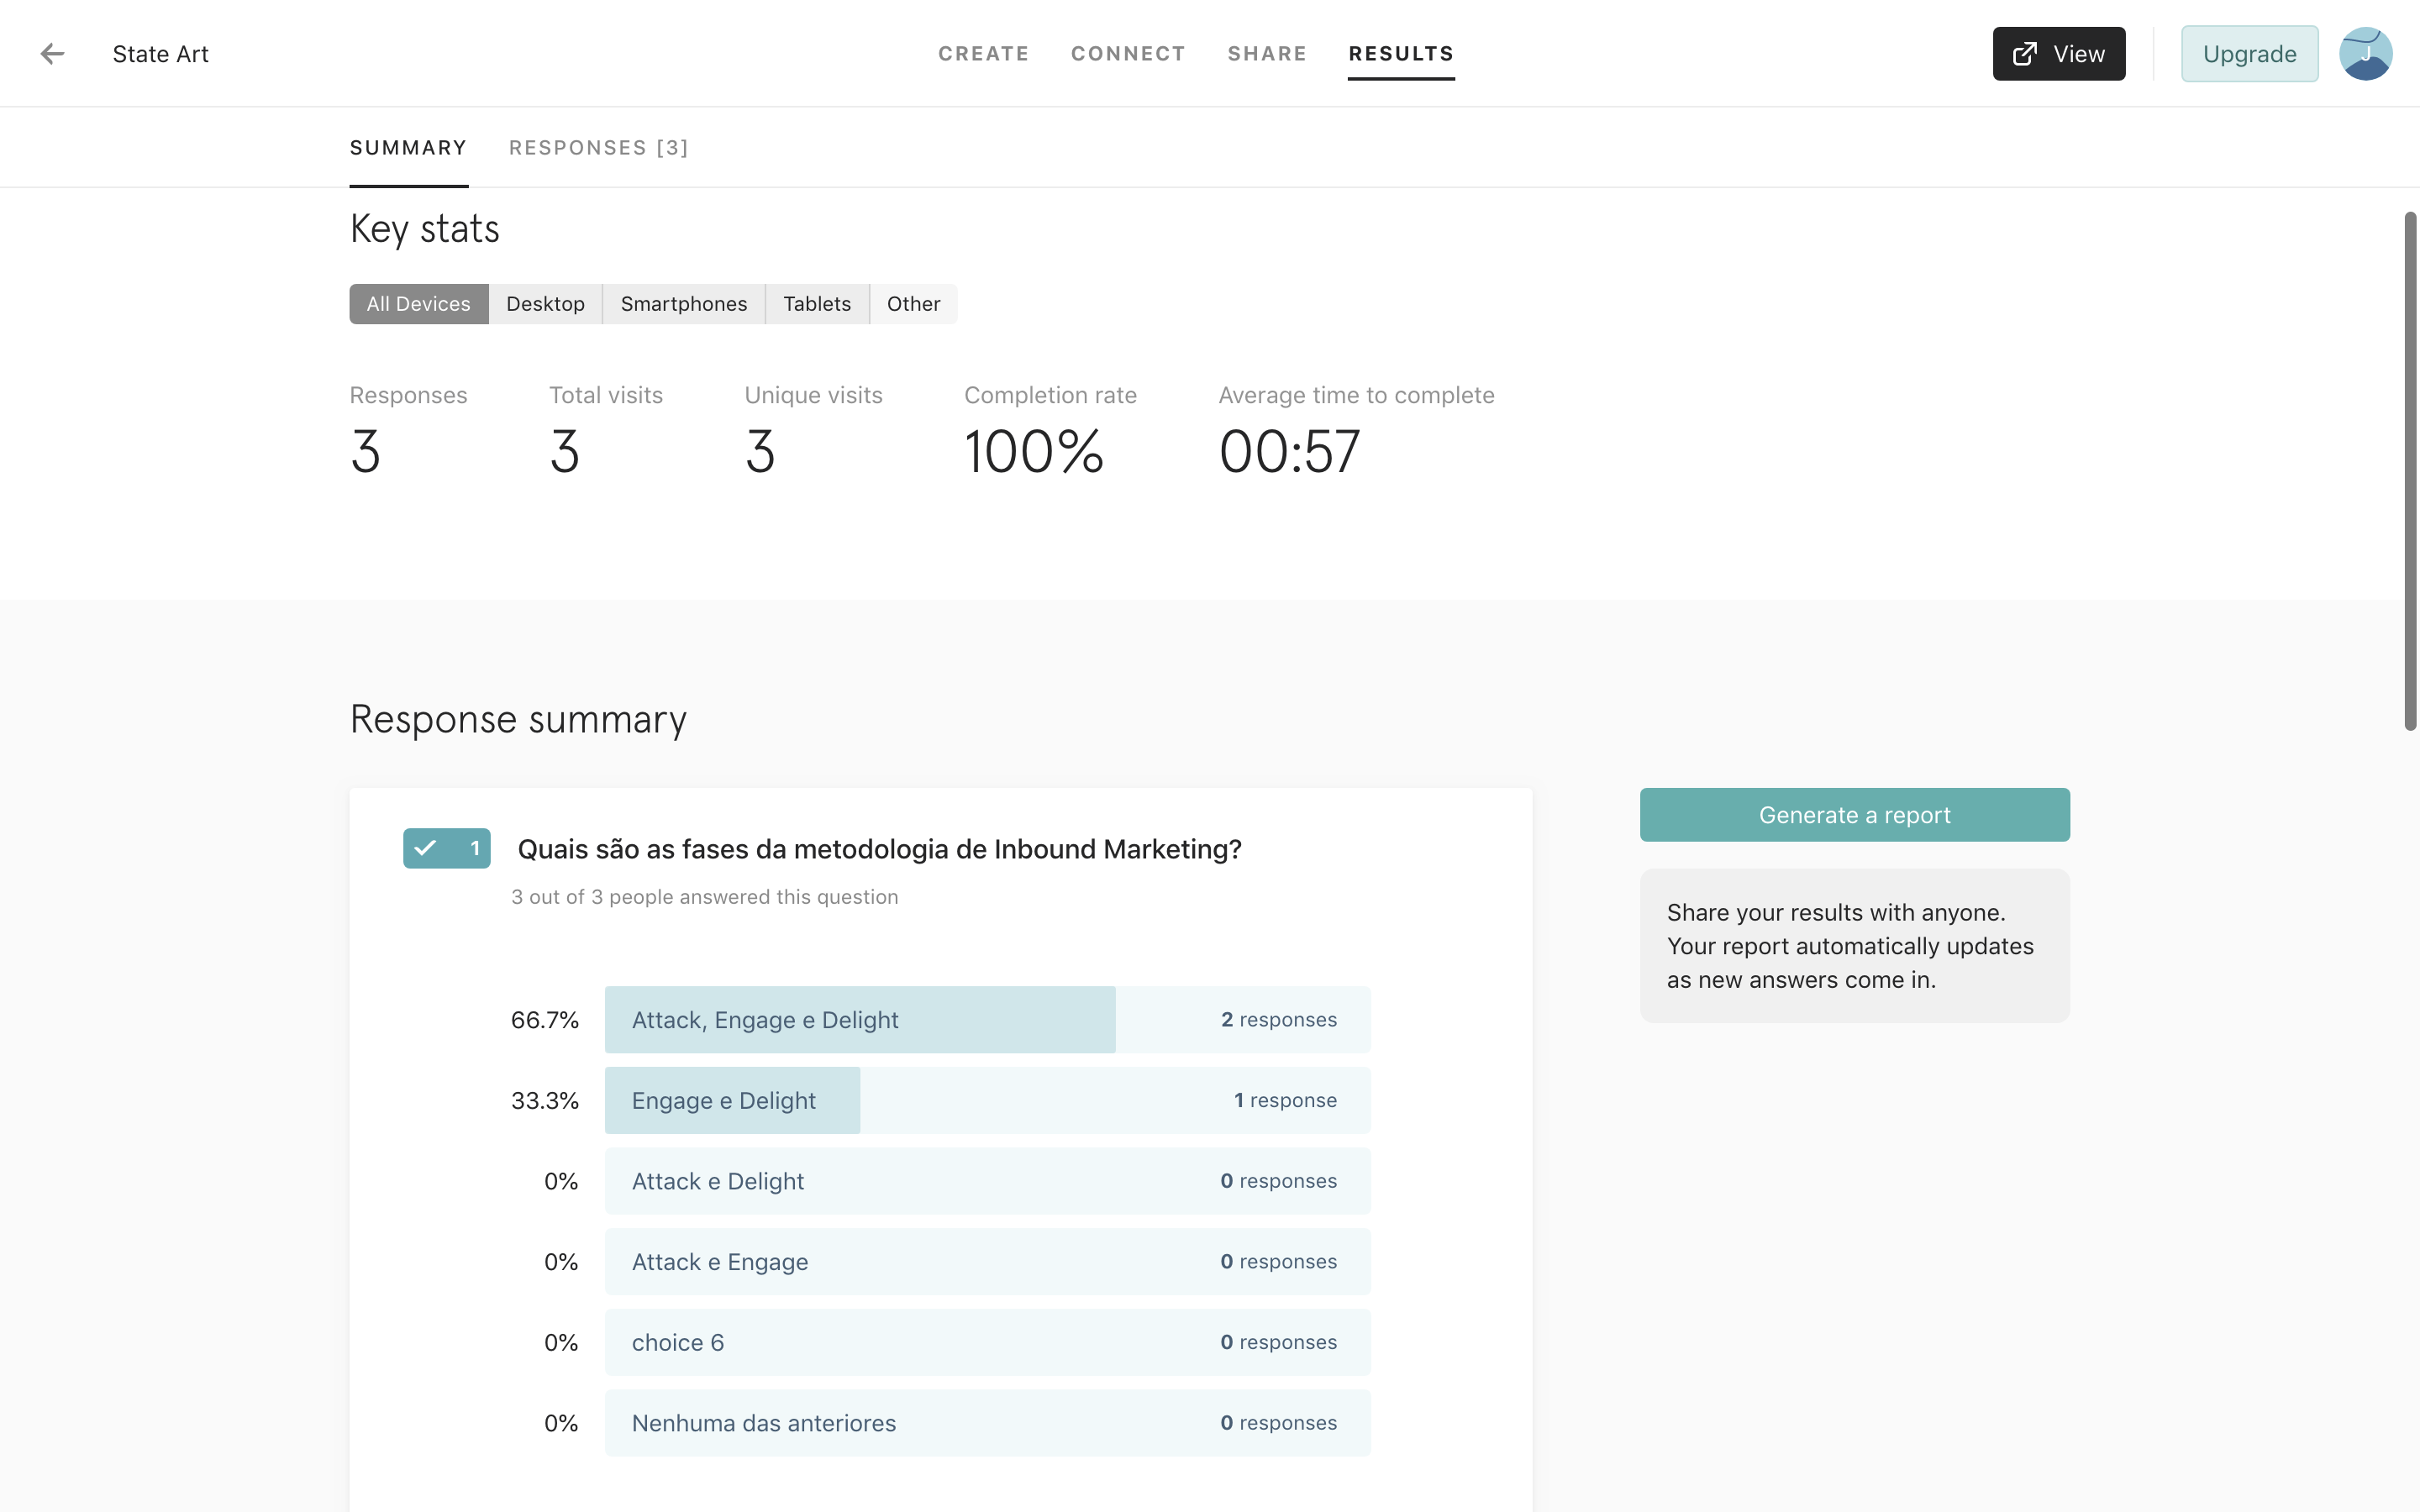
\includegraphics[width=1\textwidth]{img/tf/tf-question-results}
		\caption{Typeform - Analise de resultados}
		\label{fig:tf-question-results}
	\end{center}
\end{figure}



\section{Google Form}
\label{googleform}

O Google Form é uma aplicação de adminstração de inquéritos que está incluída no Google Drive office juntamente com o Google Docs\cite{gdocs}, Google Sheets e Google Slides\cite{gslides}. Esta ferramenta permite recolher informações do público alvo através de formulários e inquéritos personalizados e automaticamente exportar os dados para uma \textit{google sheet}.

Estam aplicação é totalmente gratuita, bastanto apenas criar uma conta Google para poder aceder a todas as funcionalidades da ferramenta.

Representado na Figura \ref{fig:gf-dashboard}, está o painel de controlo da conta de um utilizador, onde o mesmo pode visualizar os formulários com que interagiu recentemente. Por cima dos formulários recentes temos o butão para criar um novo formulário juntamente com alguns \textit{templates}/recomendações de formulários.

\newpage

\begin{figure}[ht!]
	\begin{center}
		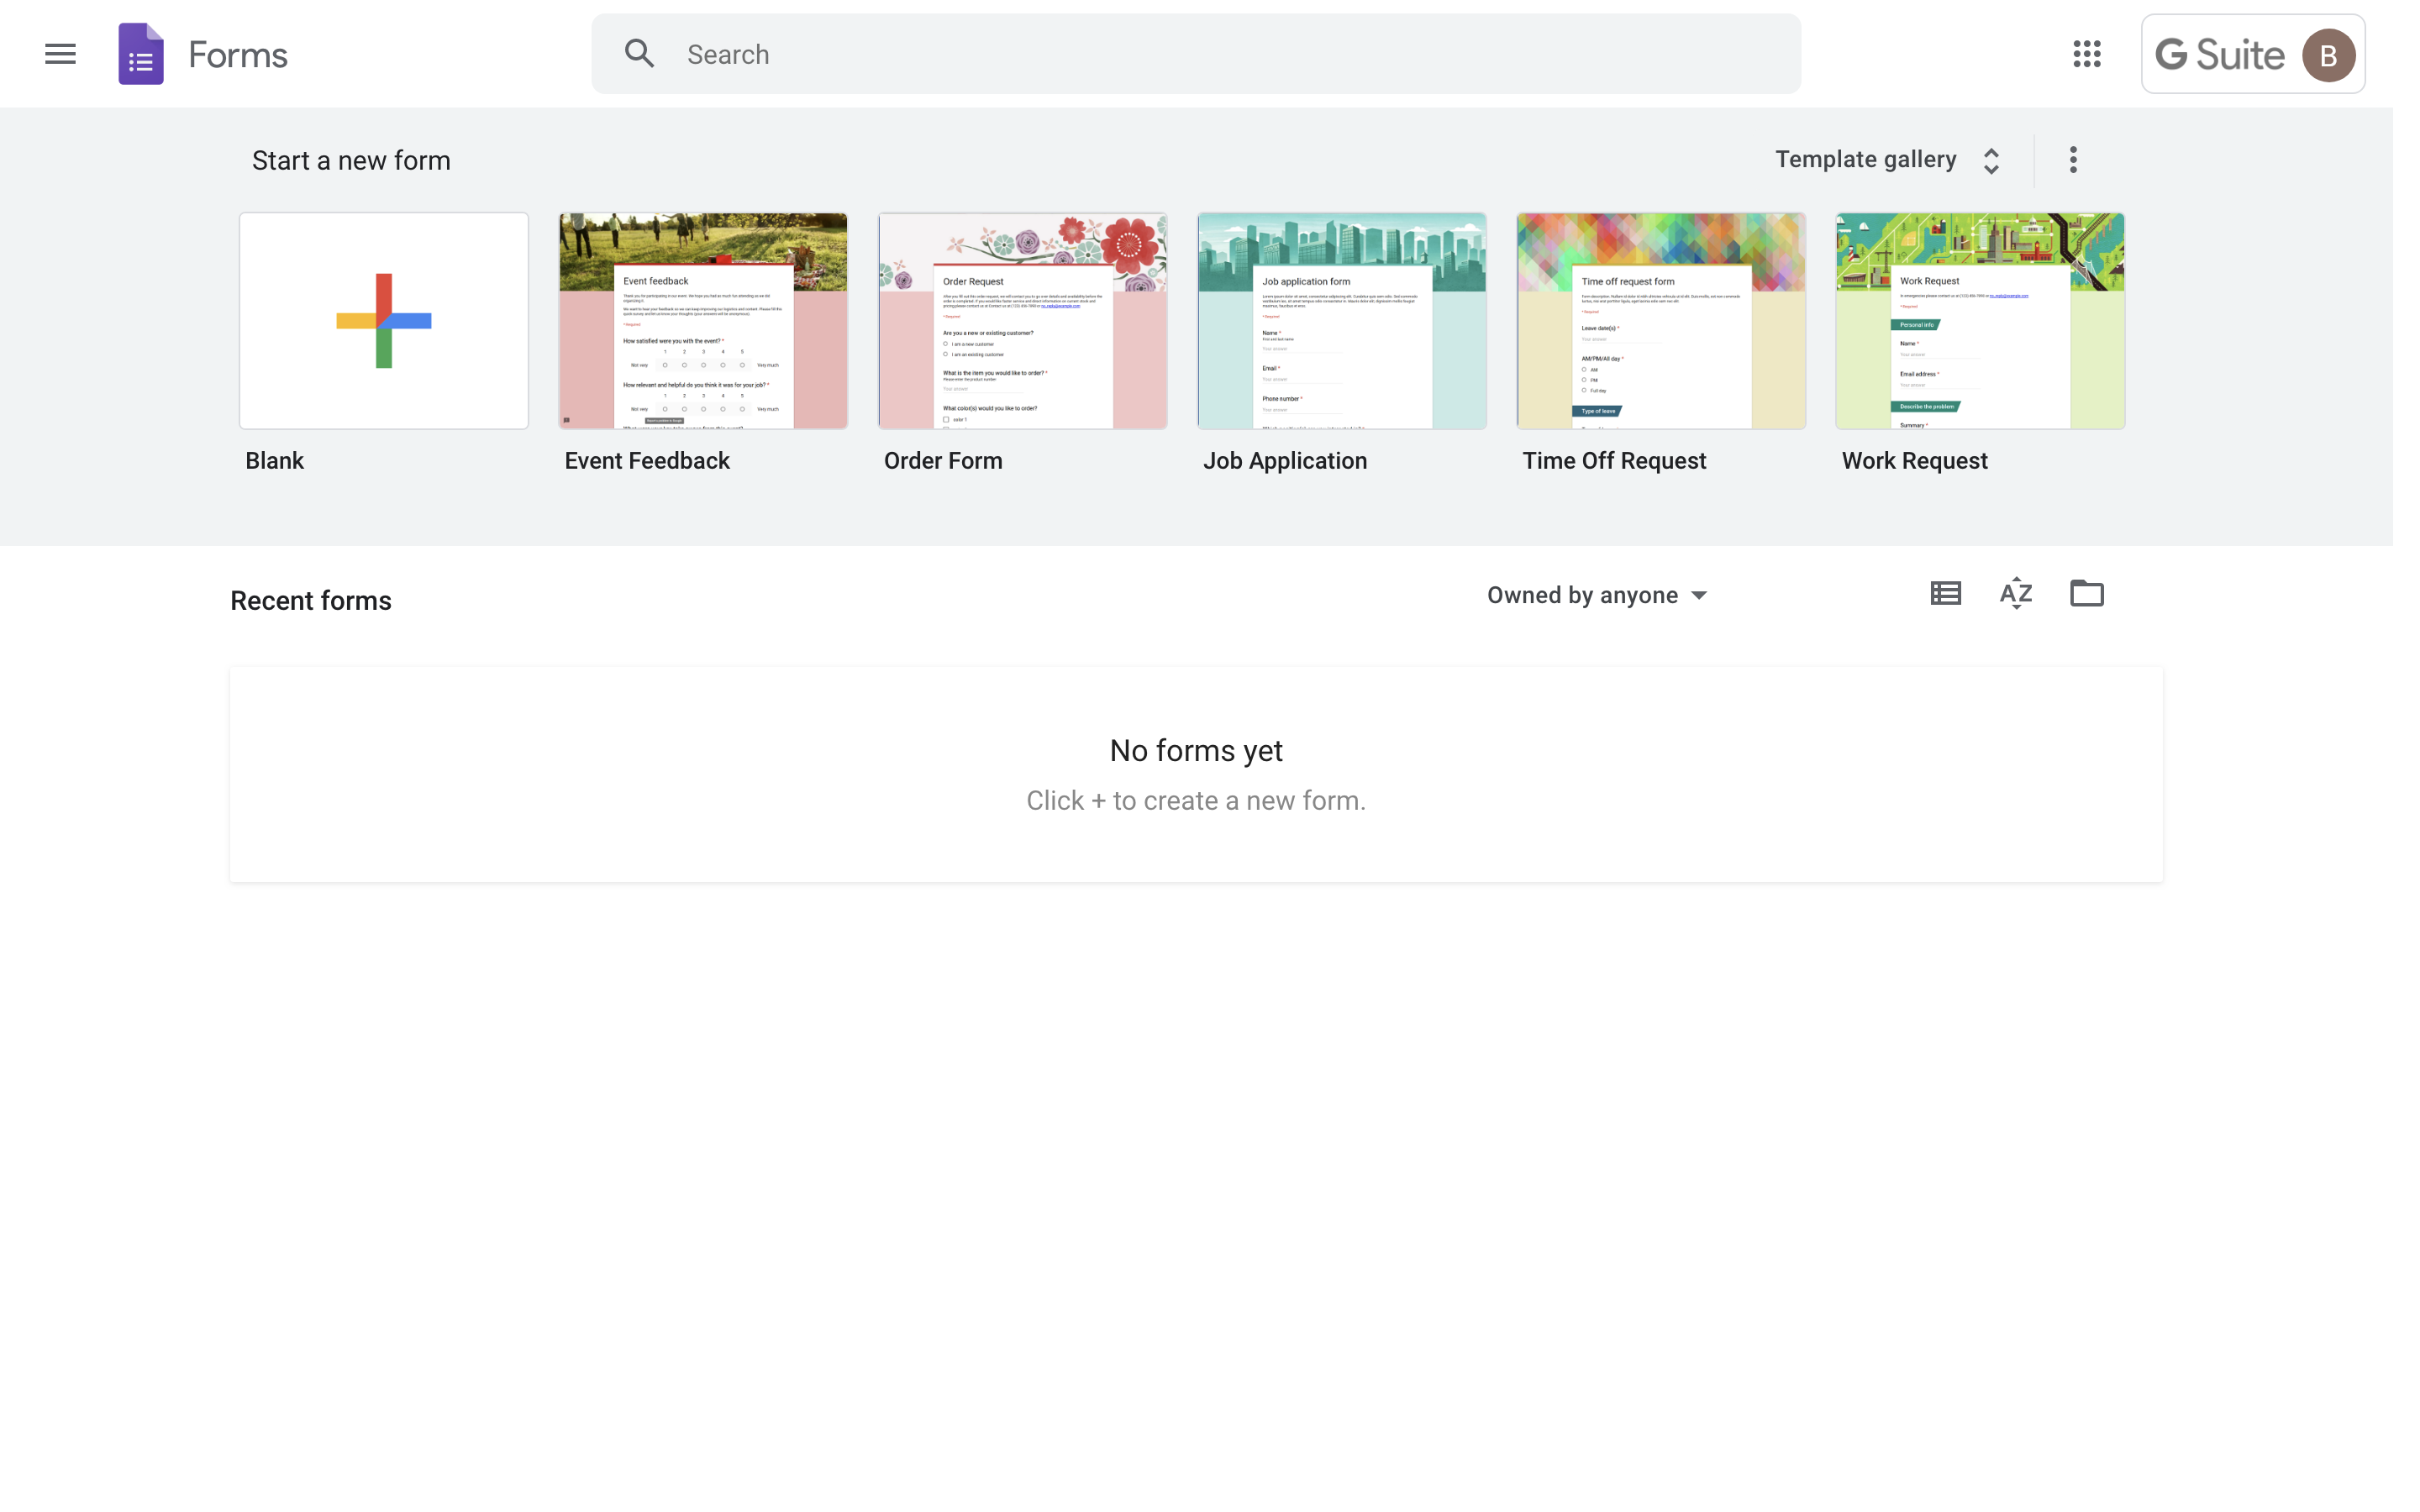
\includegraphics[width=1\textwidth]{img/gf/gf-dashboard}
		\caption{Google Form - Painel de Controlo}
		\label{fig:gf-dashboard}
	\end{center}
\end{figure}


\begin{figure}[ht!]
	\begin{center}
		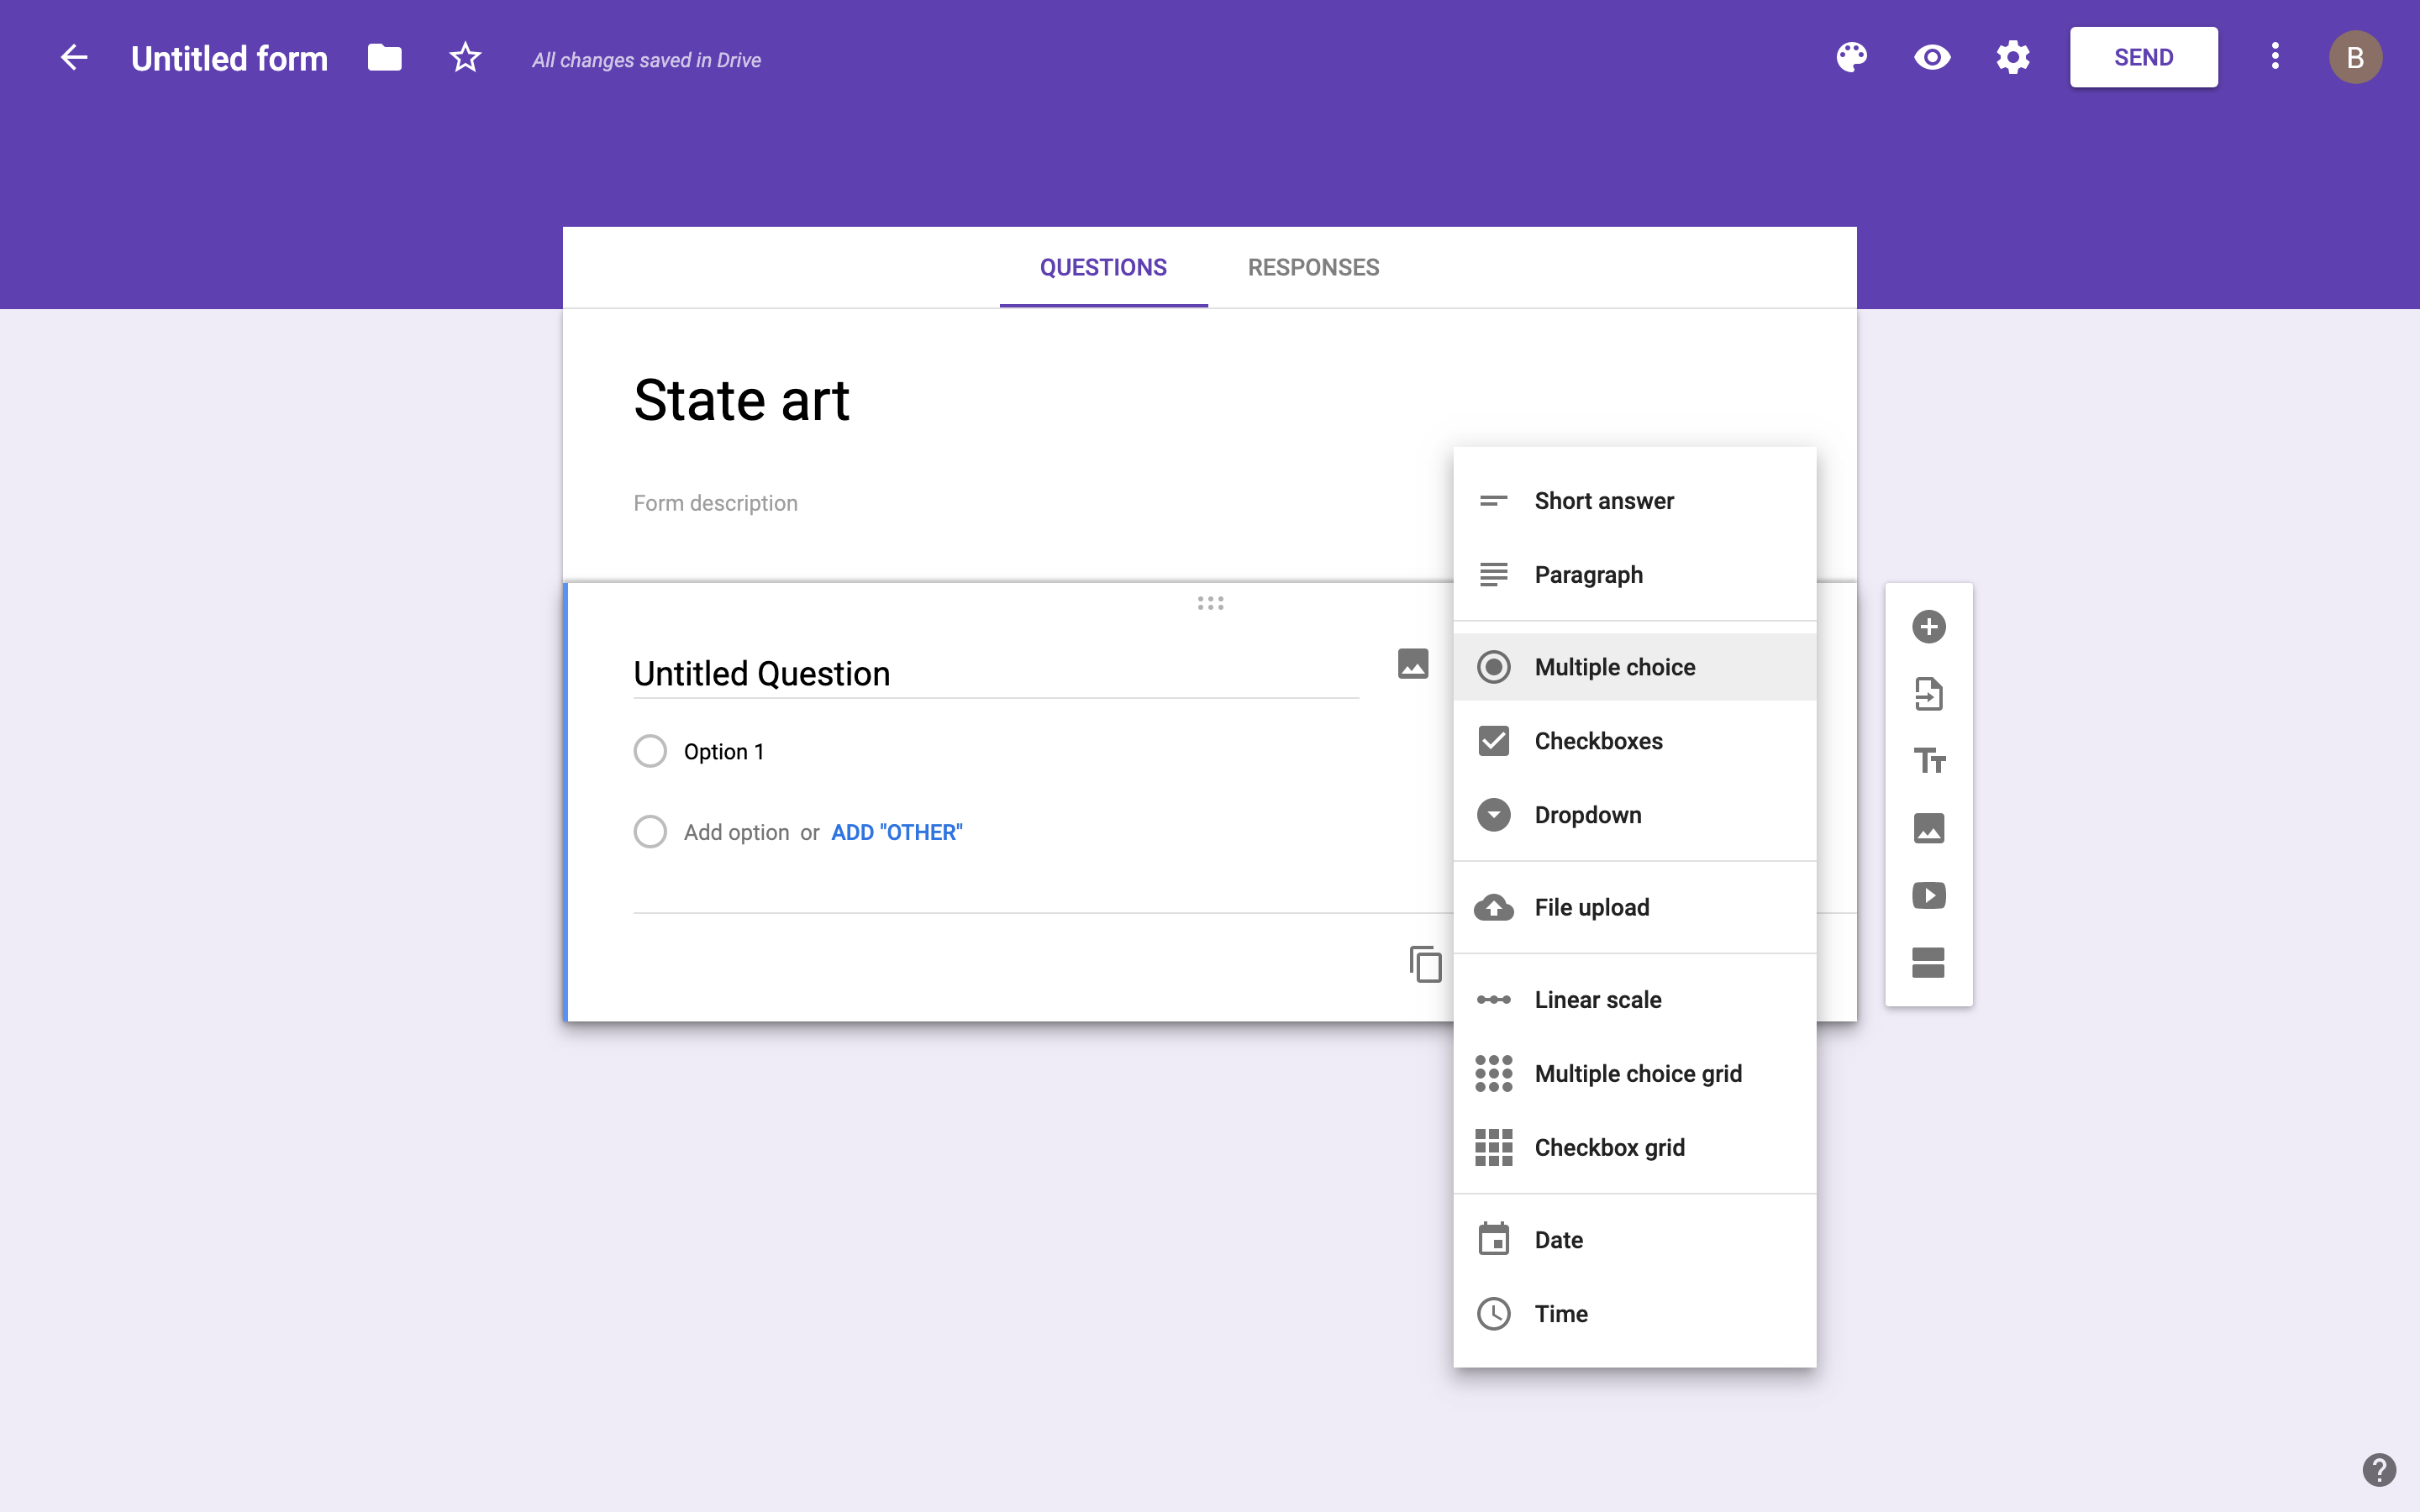
\includegraphics[width=1\textwidth]{img/gf/gf-form-q-type}
		\caption{Google Form - Tipos de perguntas}
		\label{fig:gf-form-q-type}
	\end{center}
\end{figure}

A Figura \ref{fig:gf-form-q-type} demonstra a criação de um formulário do zero. Há vários tipo de perguntas que a aplicação permite adicionar ao formulário e, apesar de se estar a criar um formulário novo, o google form permite importar um ou mais formulários diferentes, ao qual o utilizador tem acesso (i. e. formulários que estão disponíveis na sua área de trabalho), selecionando apenas as perguntas que deseja importar. Como podemos ver nas Figuras \ref{fig:gf-form-import}, \ref{fig:gf-form-import-select} e \ref{fig:gf-form-imported} as perguntas importadas foram colocadas na posição escolhida, que neste caso foi no final do formulário.

\begin{figure}[h!]
	\begin{center}
		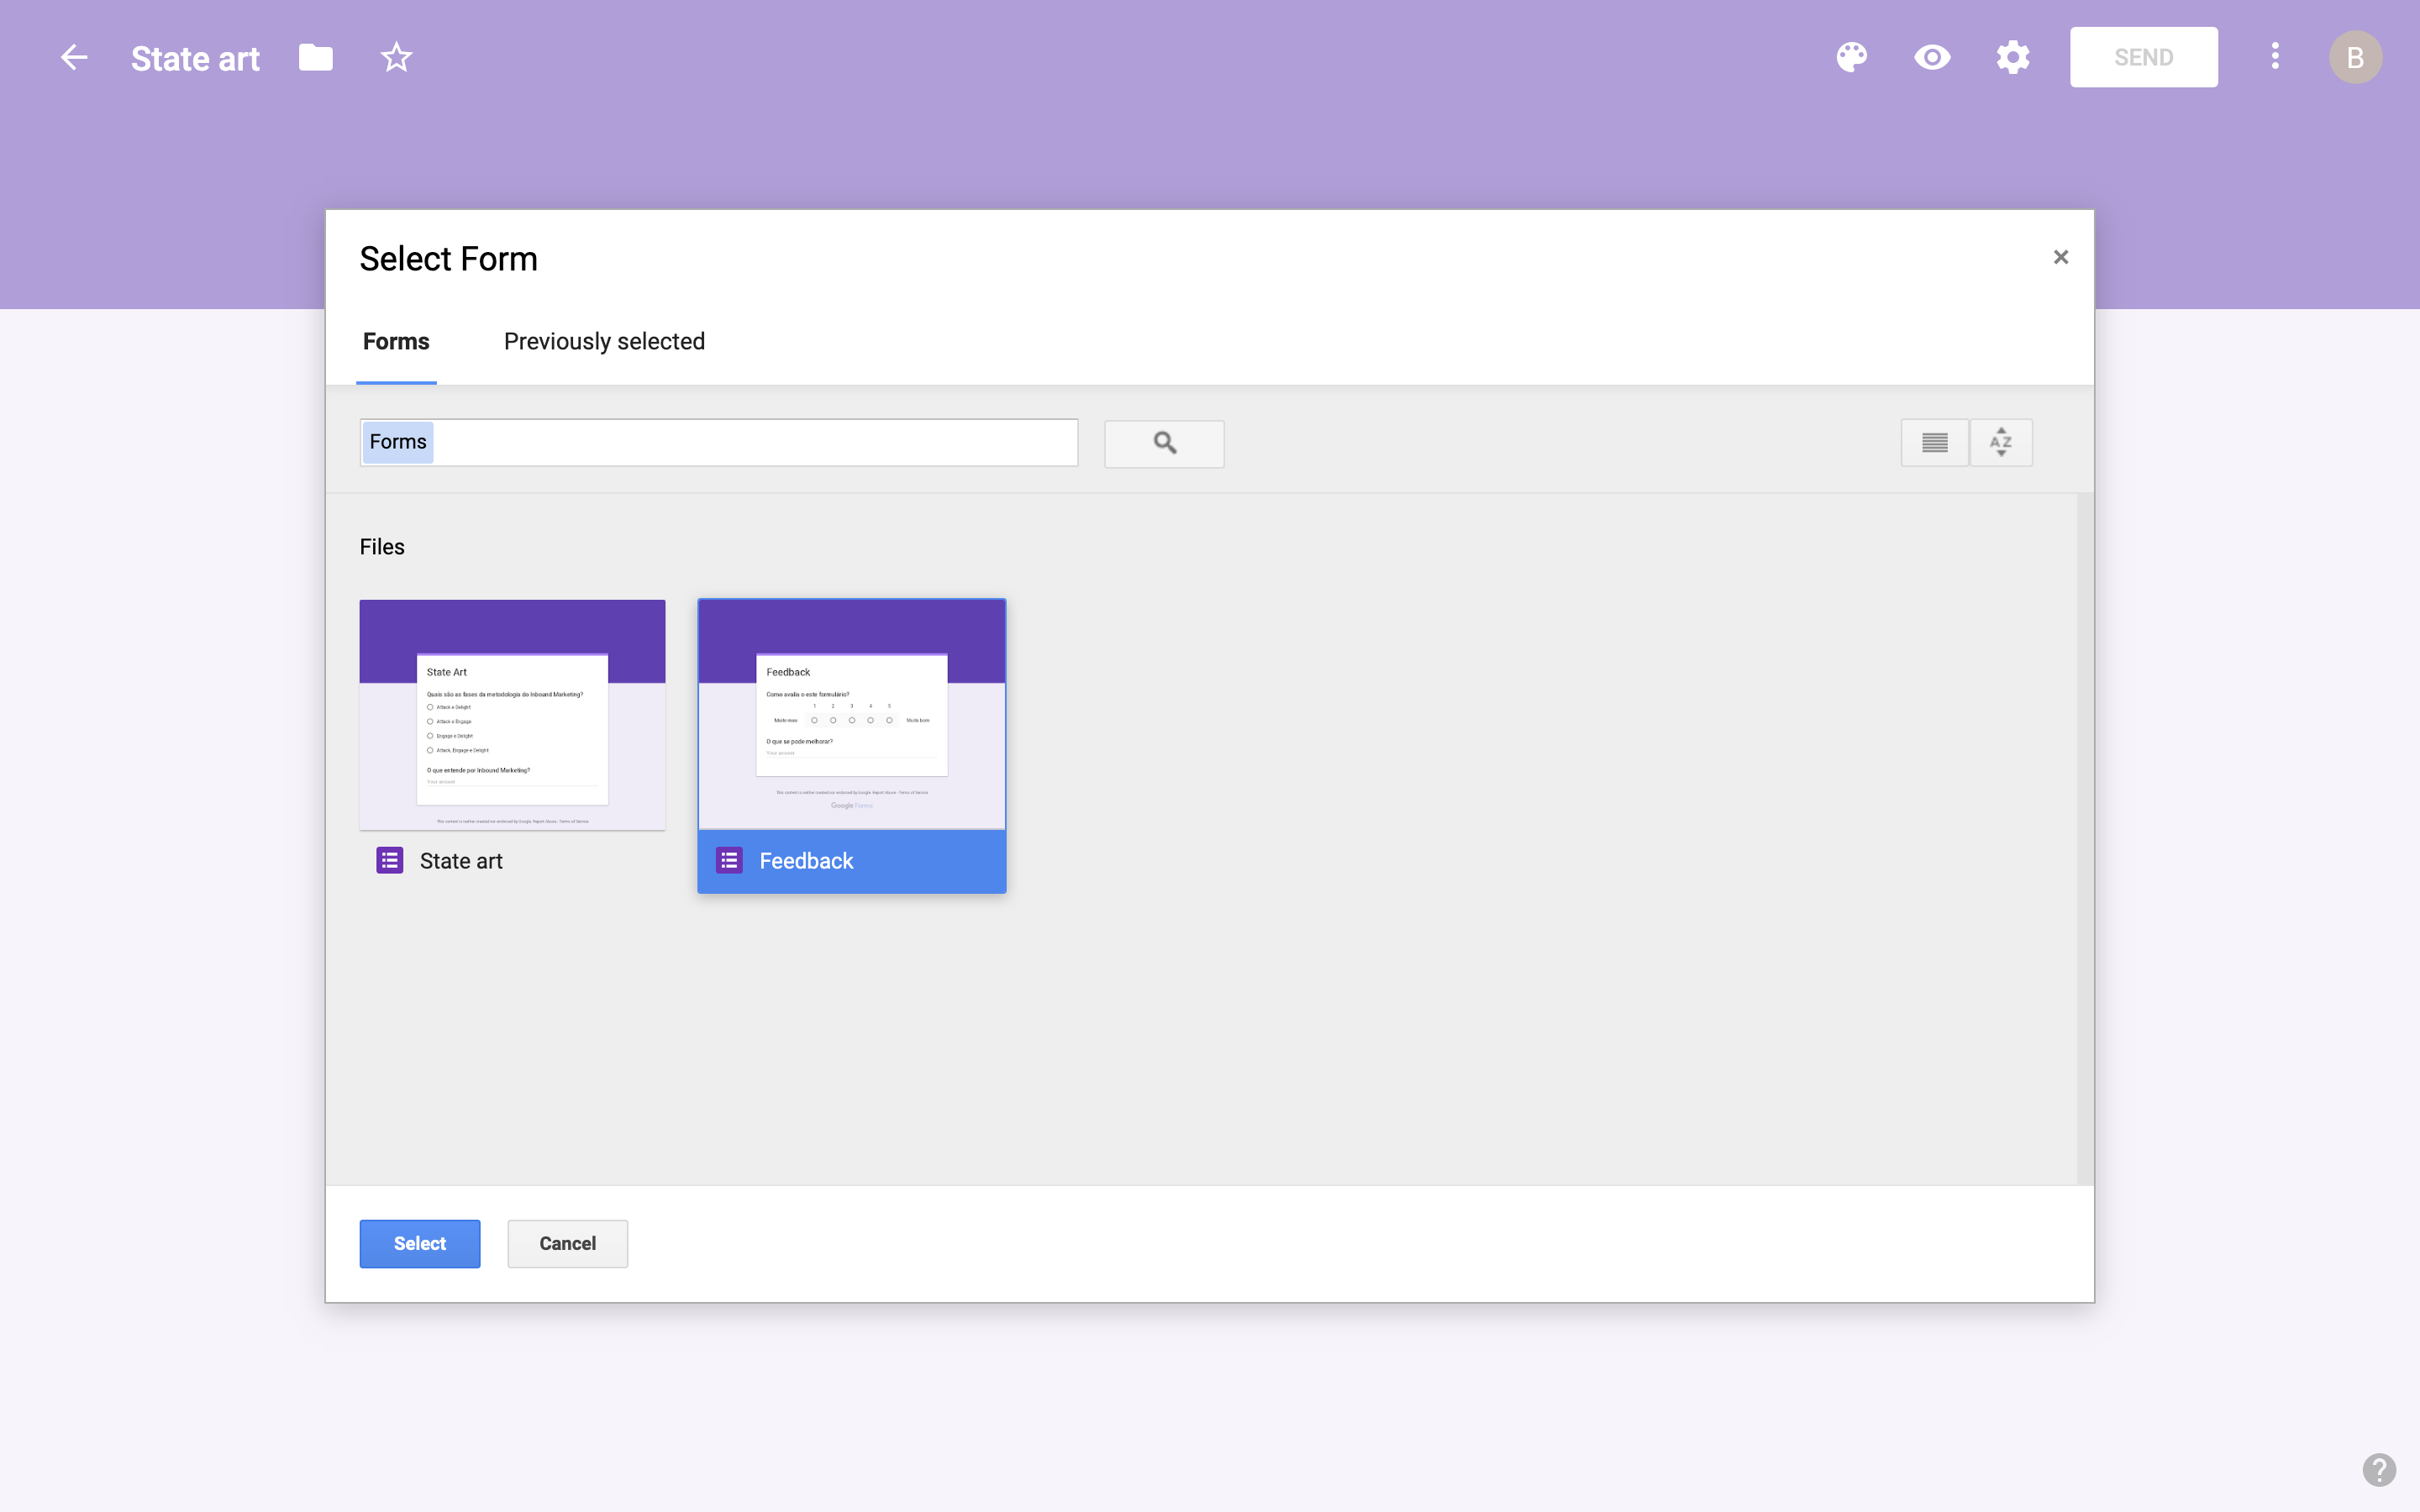
\includegraphics[width=1\textwidth]{img/gf/gf-form-import}
		\caption{Google Form - Importar formulário}
		\label{fig:gf-form-import}
	\end{center}
\end{figure}

\begin{figure}[h!]
	\begin{center}
		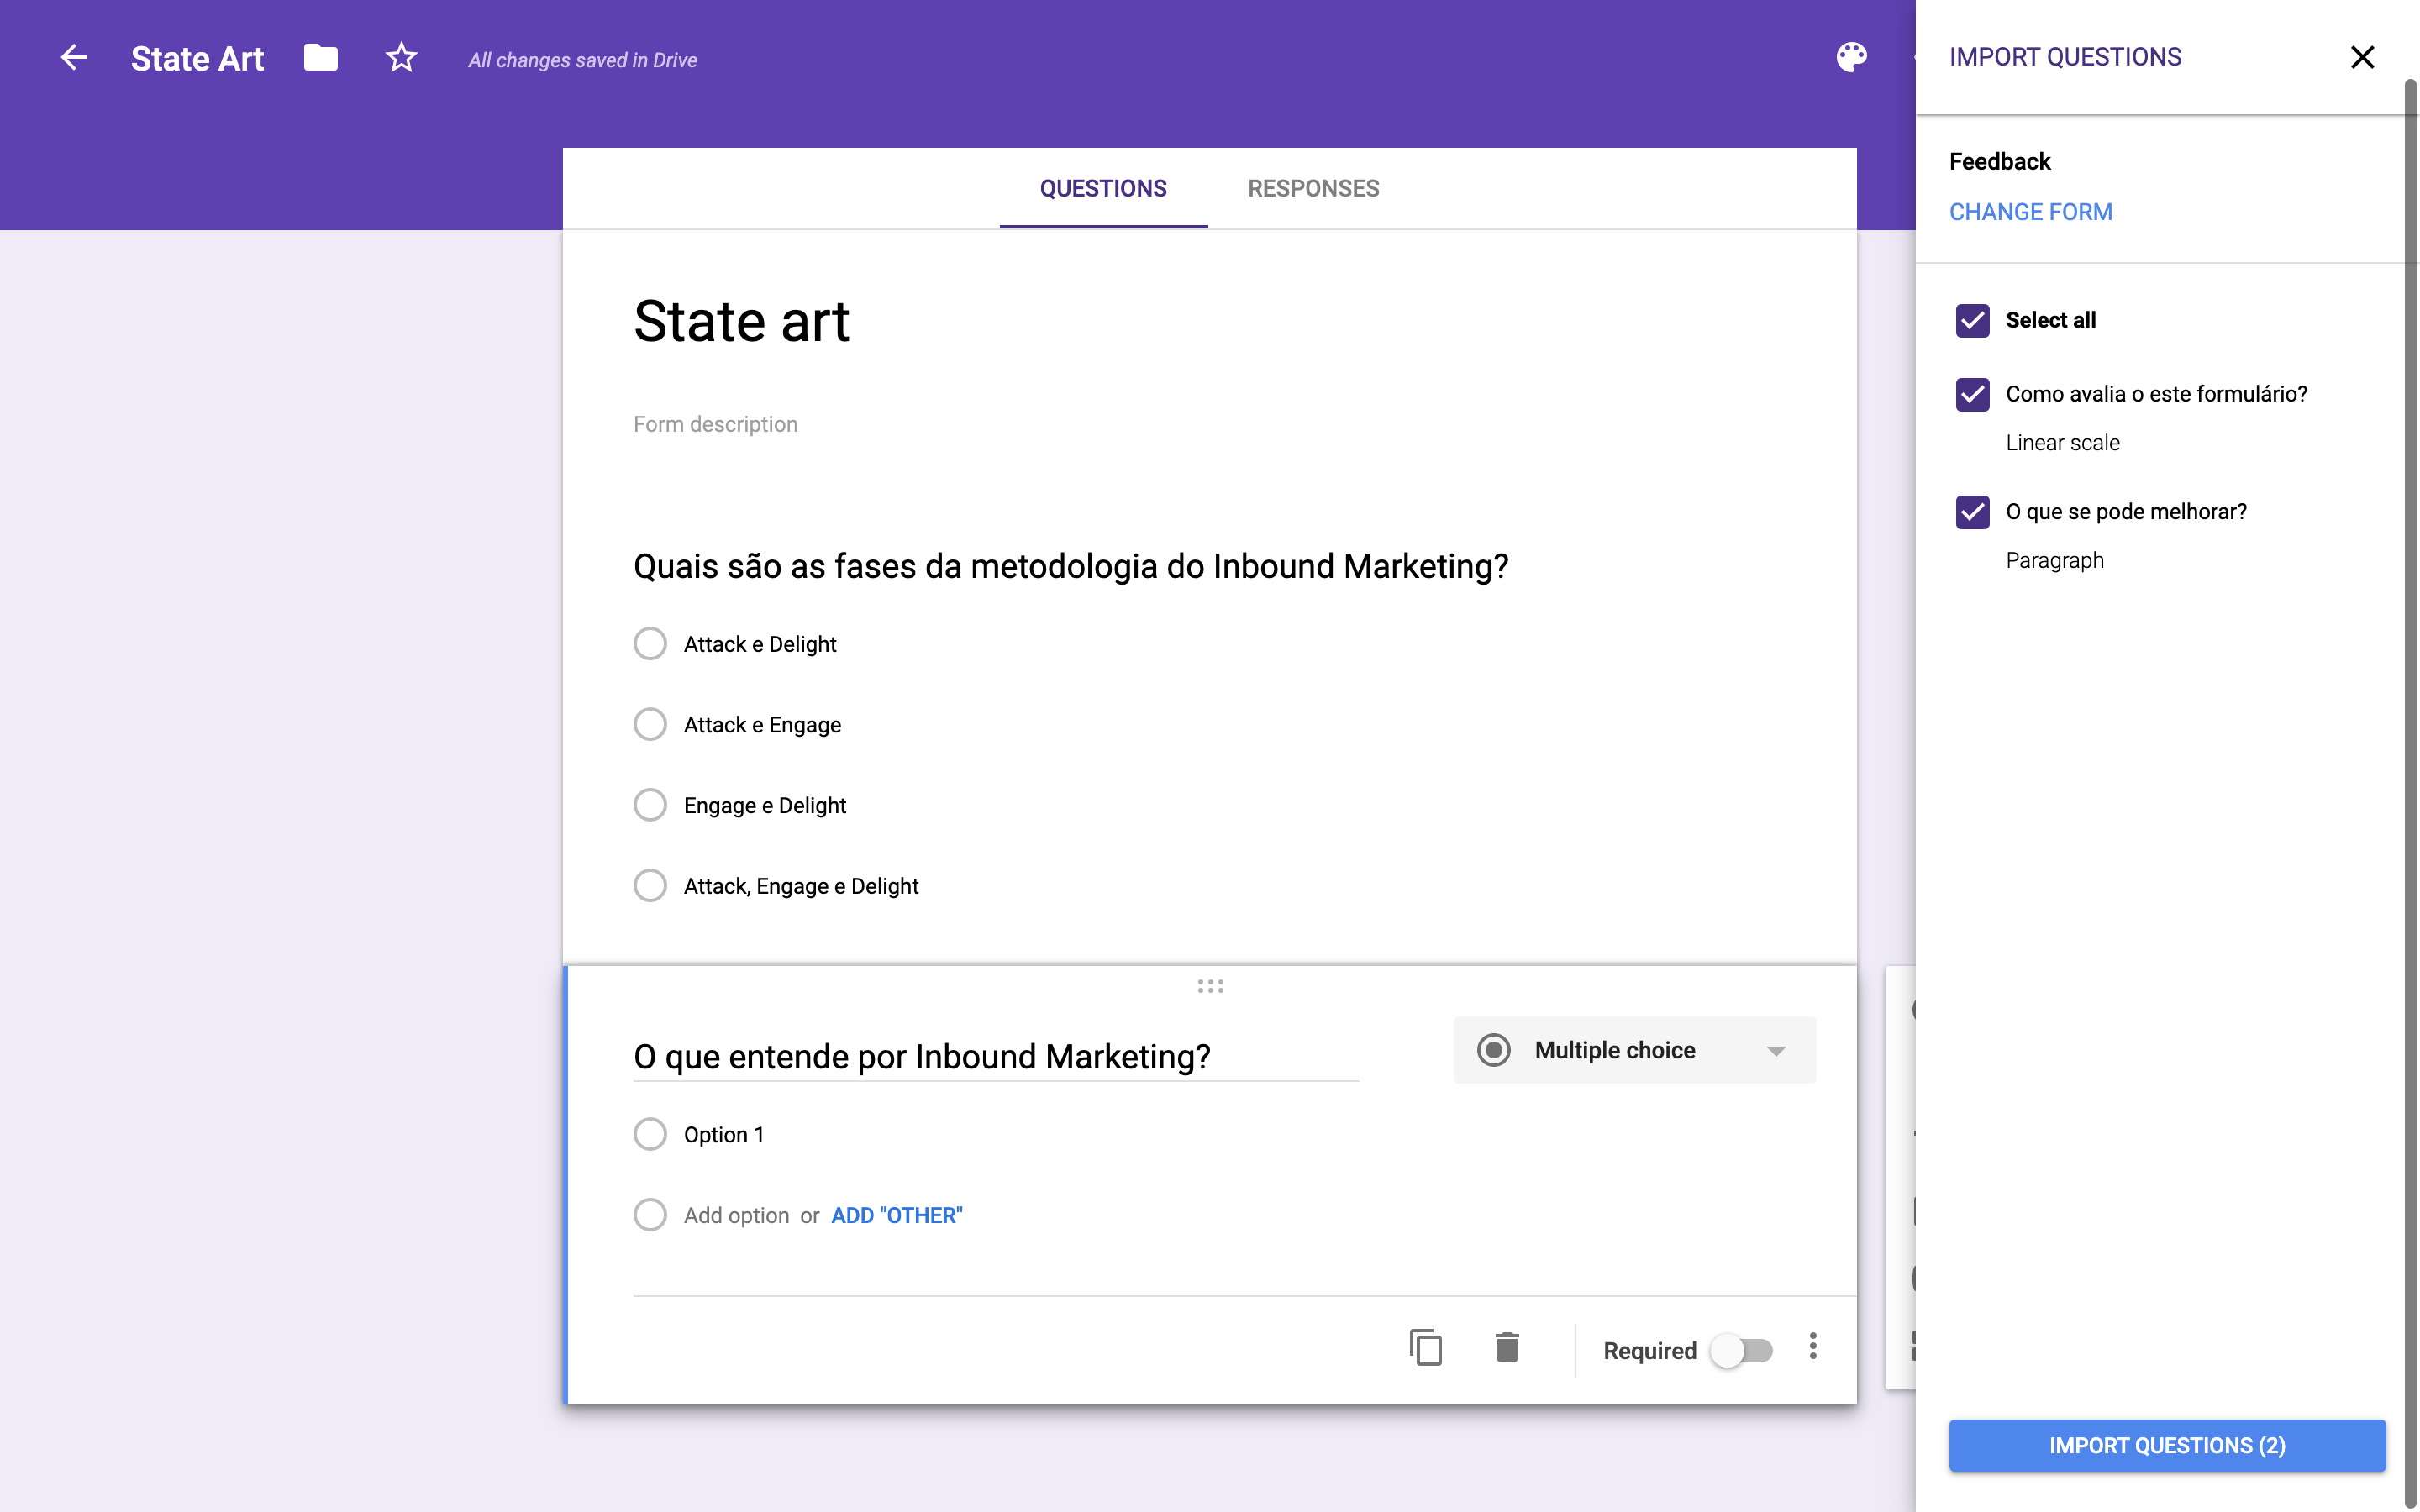
\includegraphics[width=1\textwidth]{img/gf/gf-form-import-select}
		\caption{Google Form - Selecionar perguntas a importar}
		\label{fig:gf-form-import-select}
	\end{center}
\end{figure}

\begin{figure}[h!]
	\begin{center}
		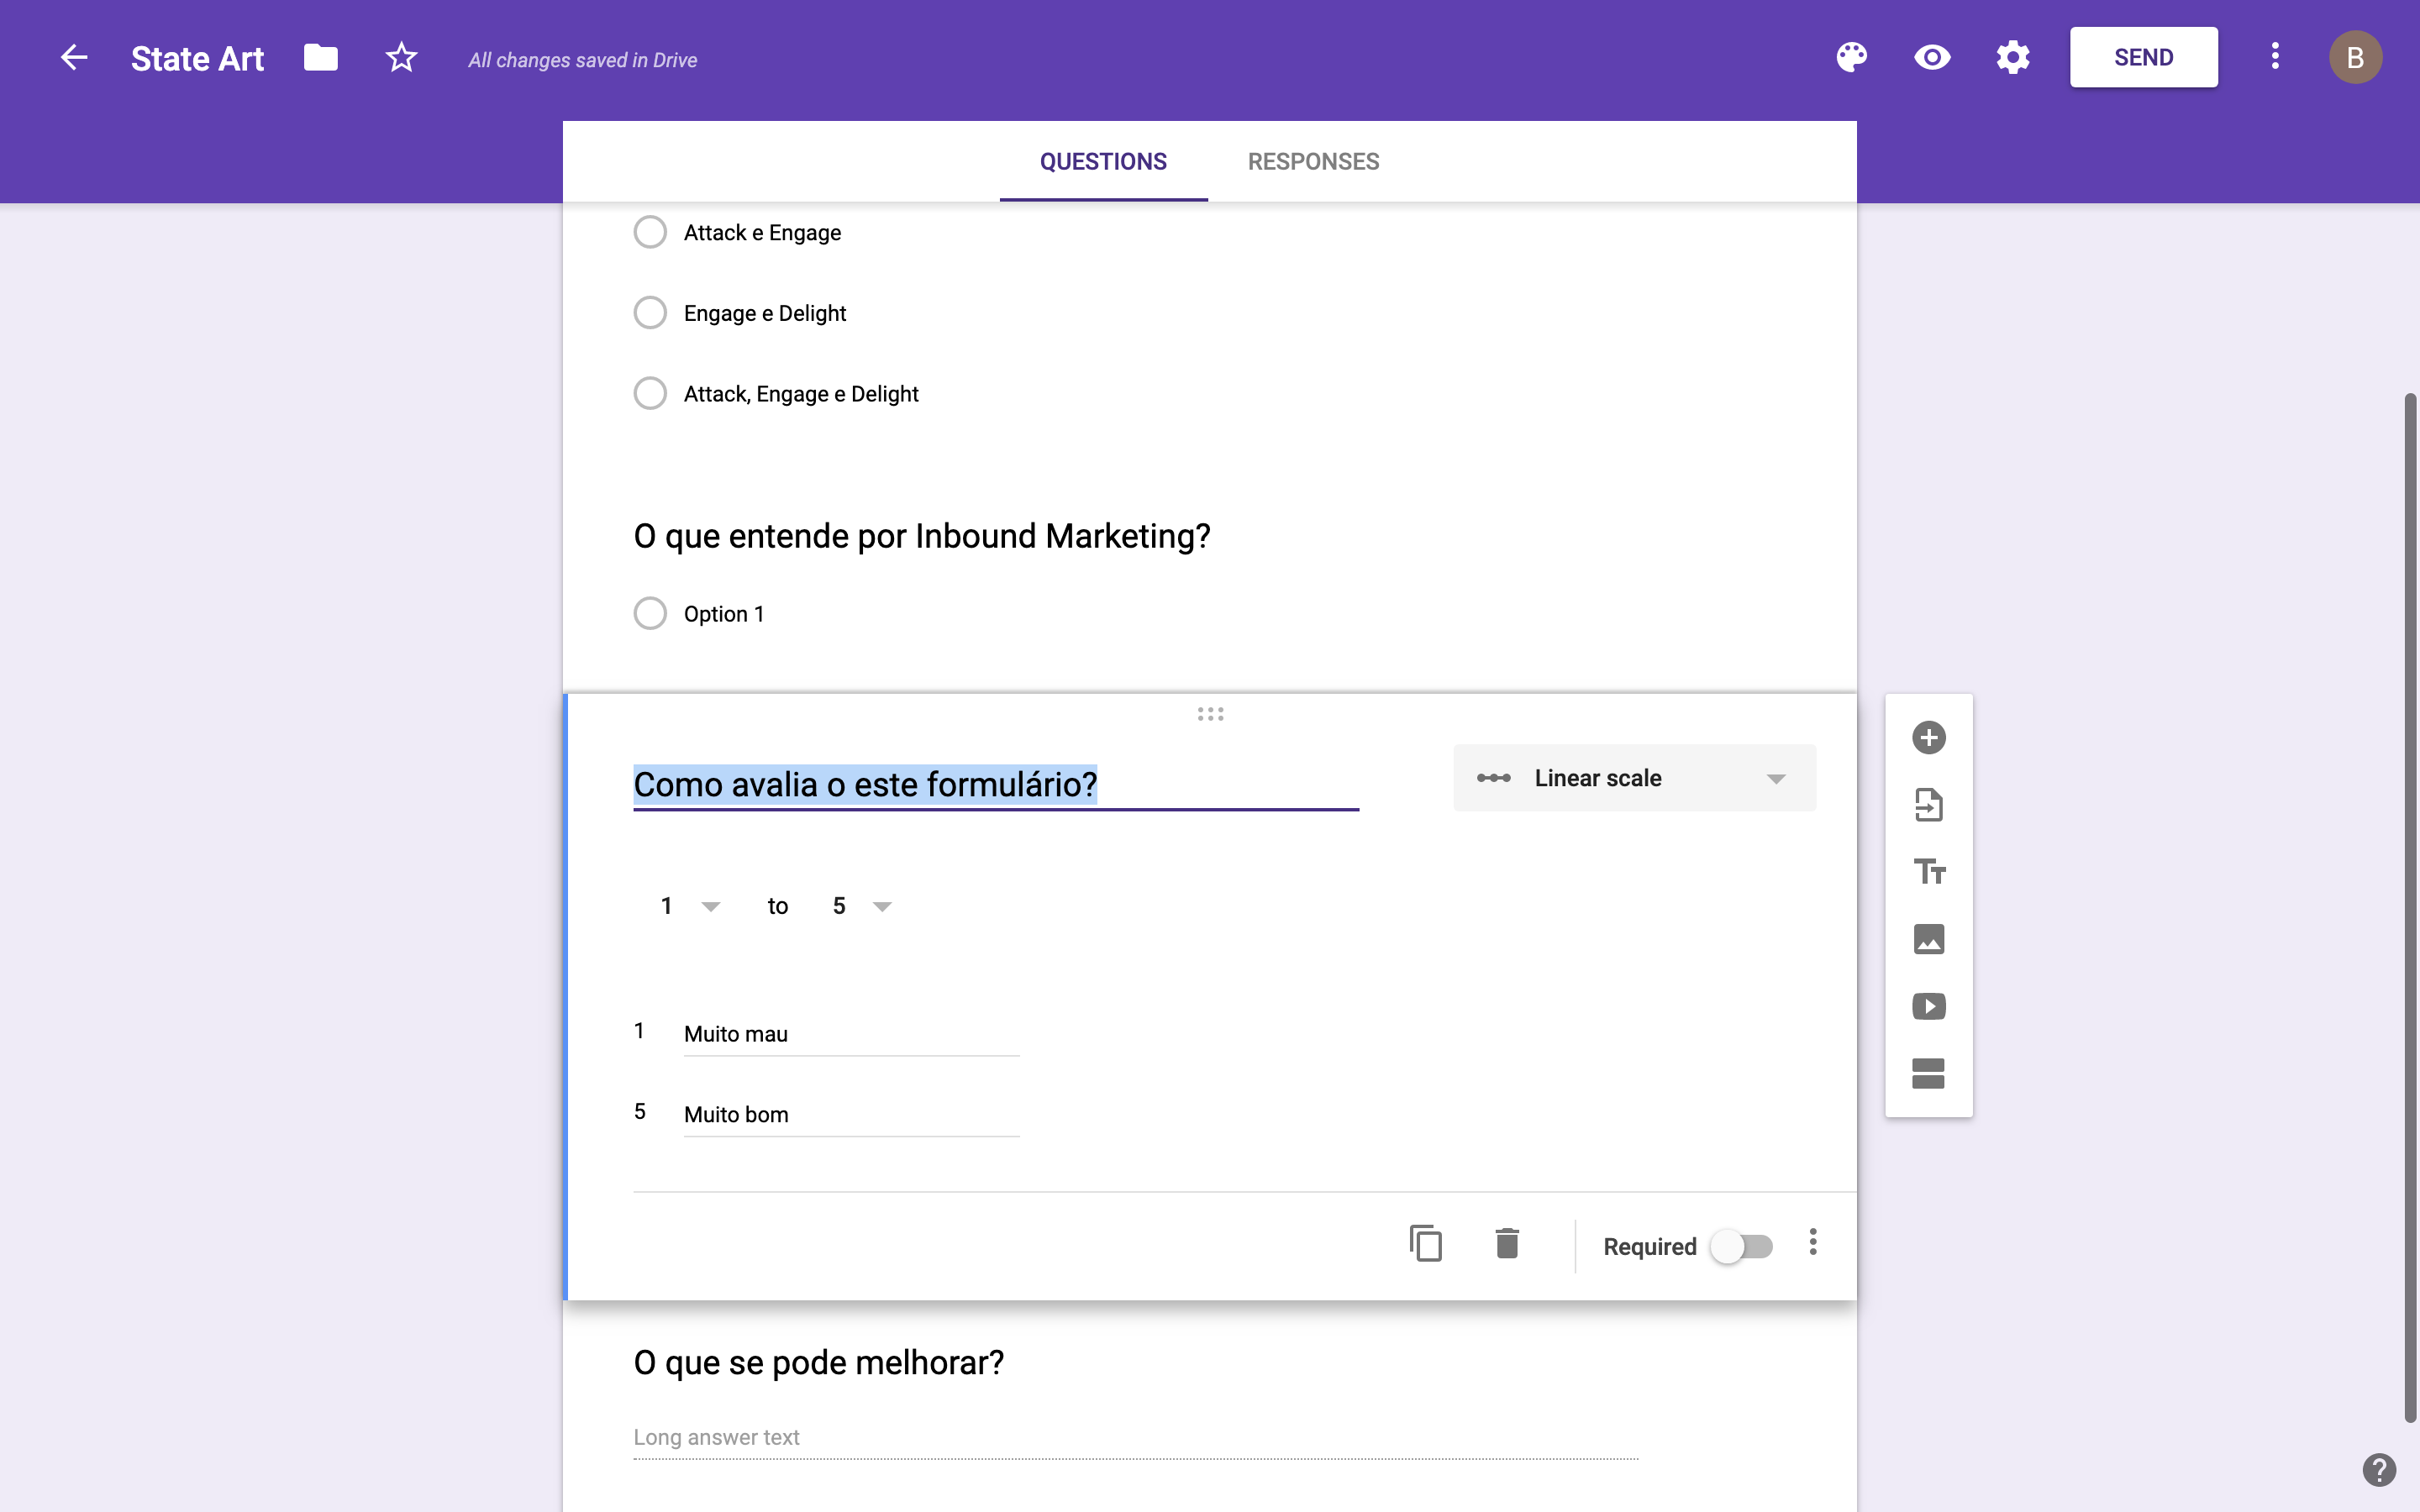
\includegraphics[width=1\textwidth]{img/gf/gf-form-imported}
		\caption{Google Form - Perguntas importadas}
		\label{fig:gf-form-imported}
	\end{center}
\end{figure}


\begin{figure}[h!]
	\begin{center}
		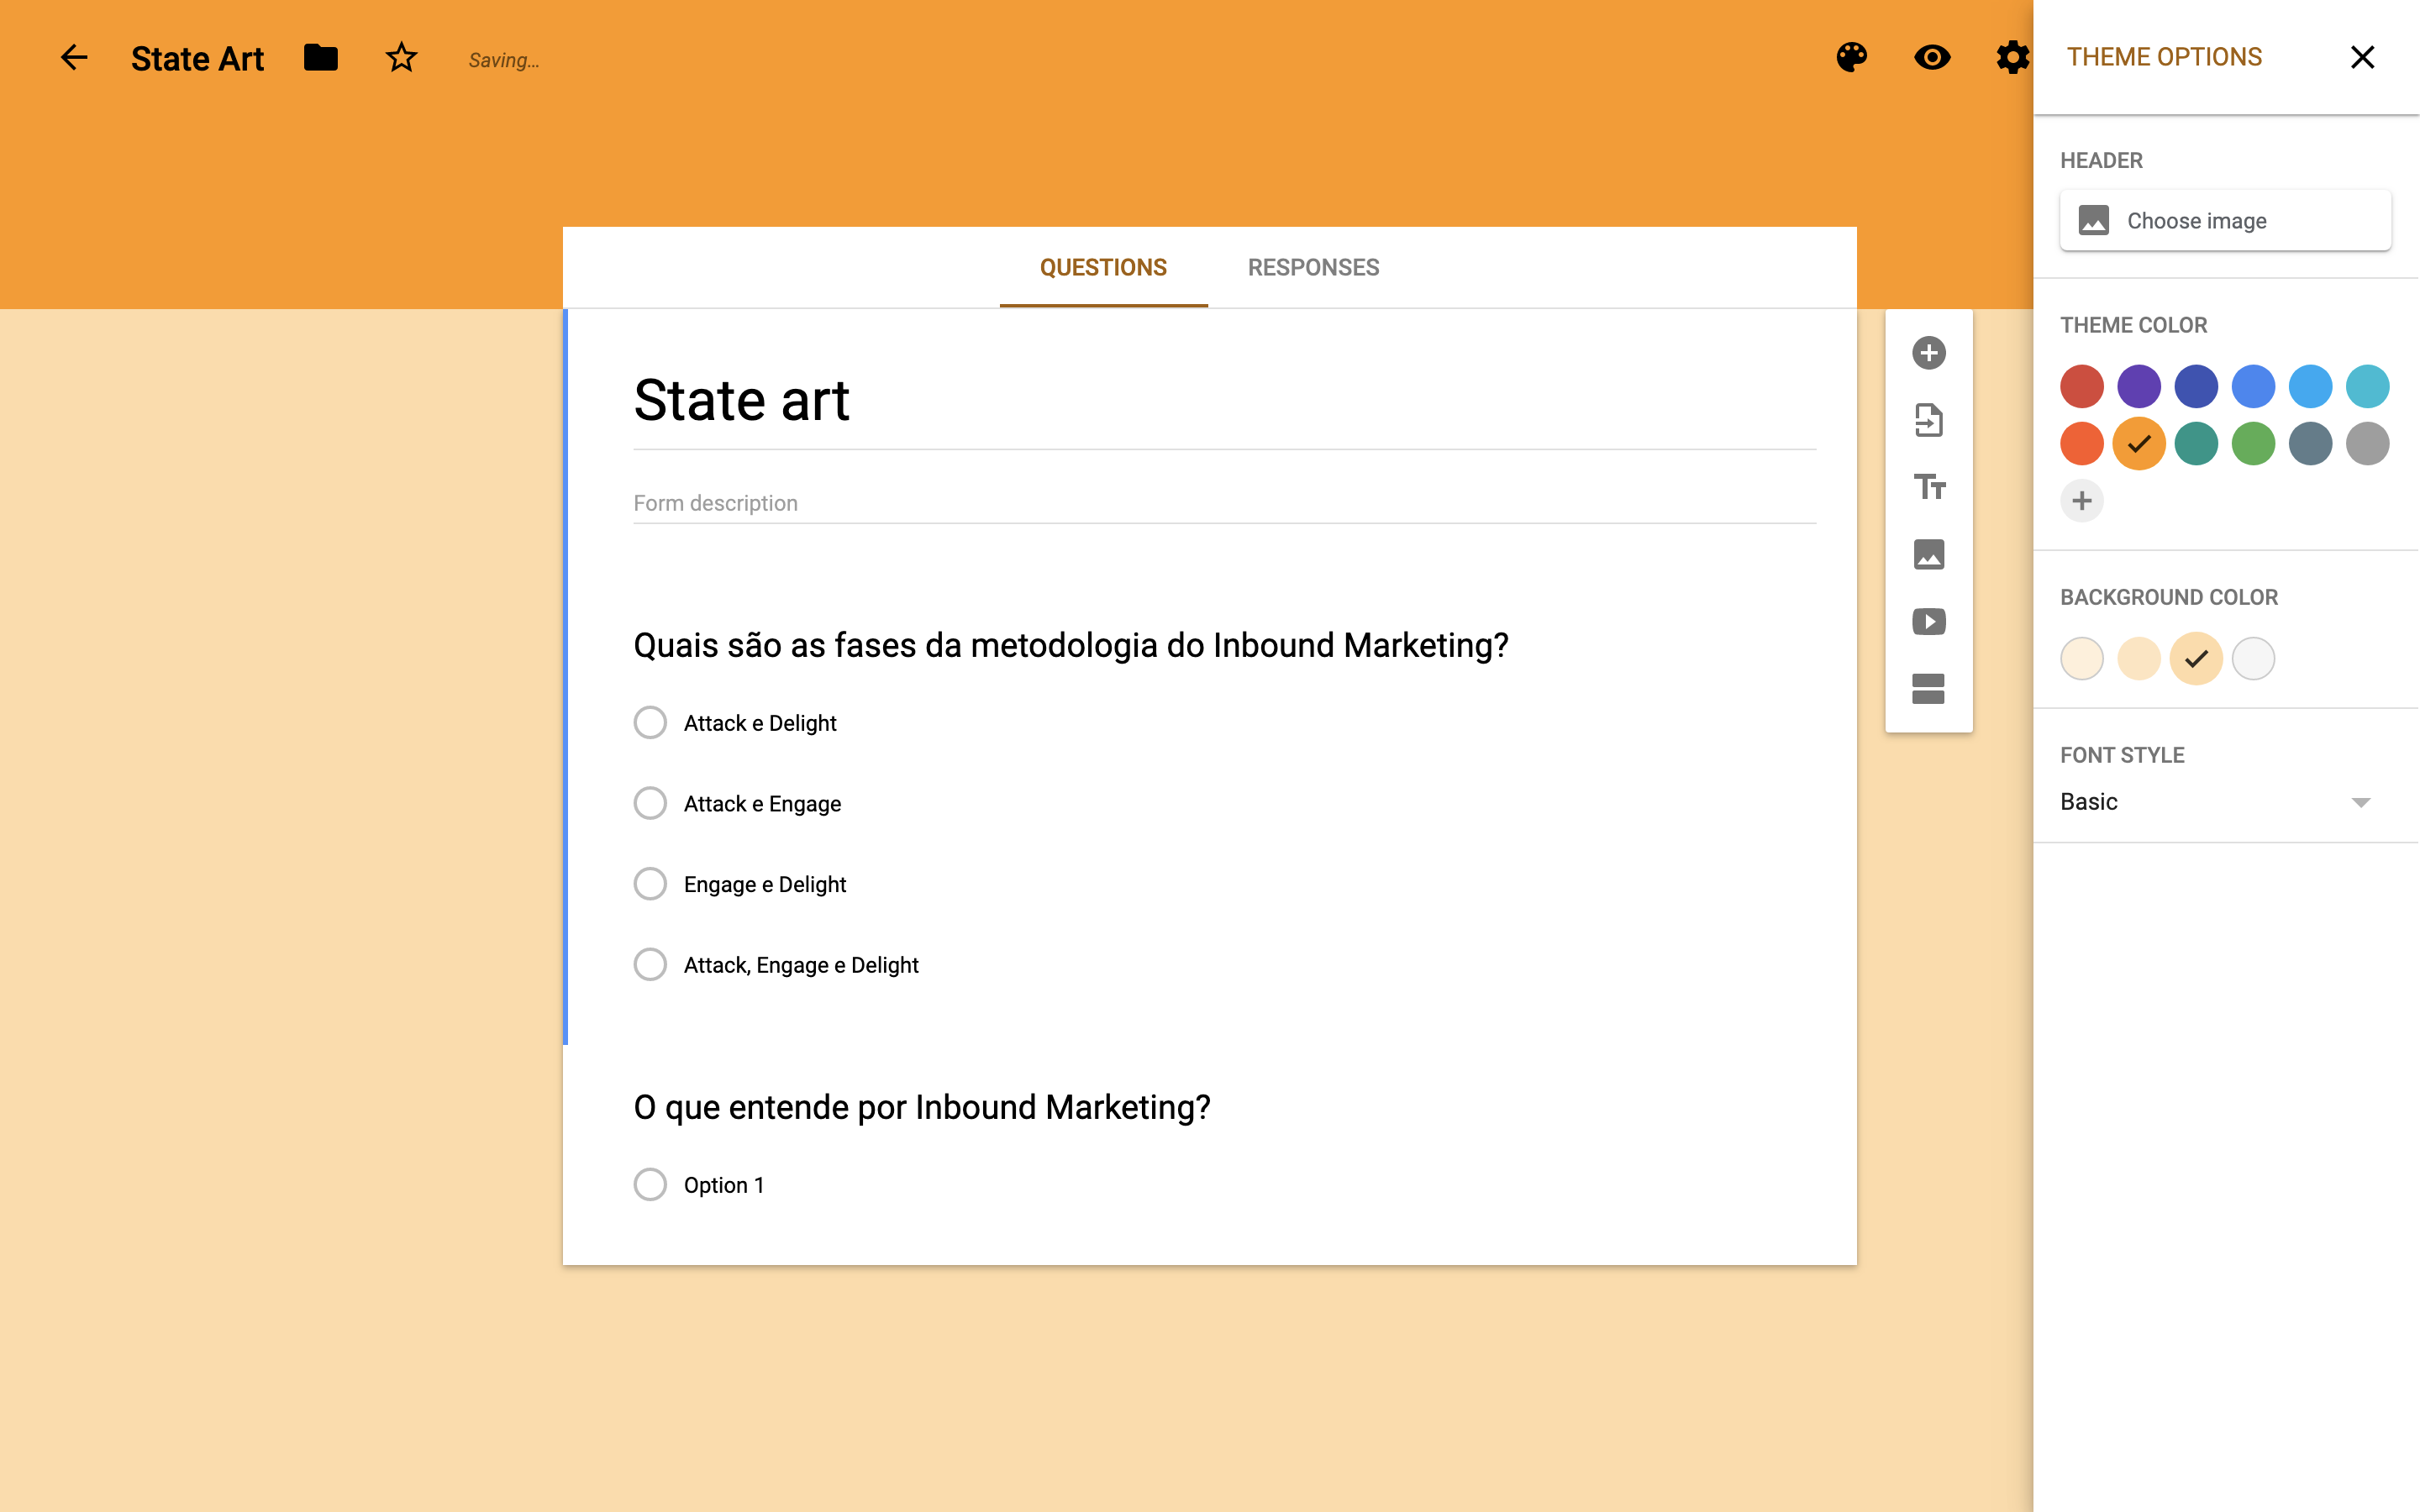
\includegraphics[width=1\textwidth]{img/gf/gf-form-design}
		\caption{Google Form - Alterar design do formulário}
		\label{fig:gf-form-design}
	\end{center}
\end{figure}

\newpage

Grande parte das plataformas e aplicações,no mercado, de criação de formulários permitem personalizar os formulários, ao gosto do utilizador, e o Google Form não é excepção. A aplicação permite alterar as definições padrão do formulário(Figuras \ref{fig:gf-form-set1}, \ref{fig:gf-form-set2} e \ref{fig:gf-form-set3}) e, apesar de se poder também personalidar o \textit{design} do formulário (\ref{fig:gf-form-design}), apens podemos alterar a cor ou imagem de fundo e fonte de texto.

\begin{figure}[ht!]
	\begin{center}
		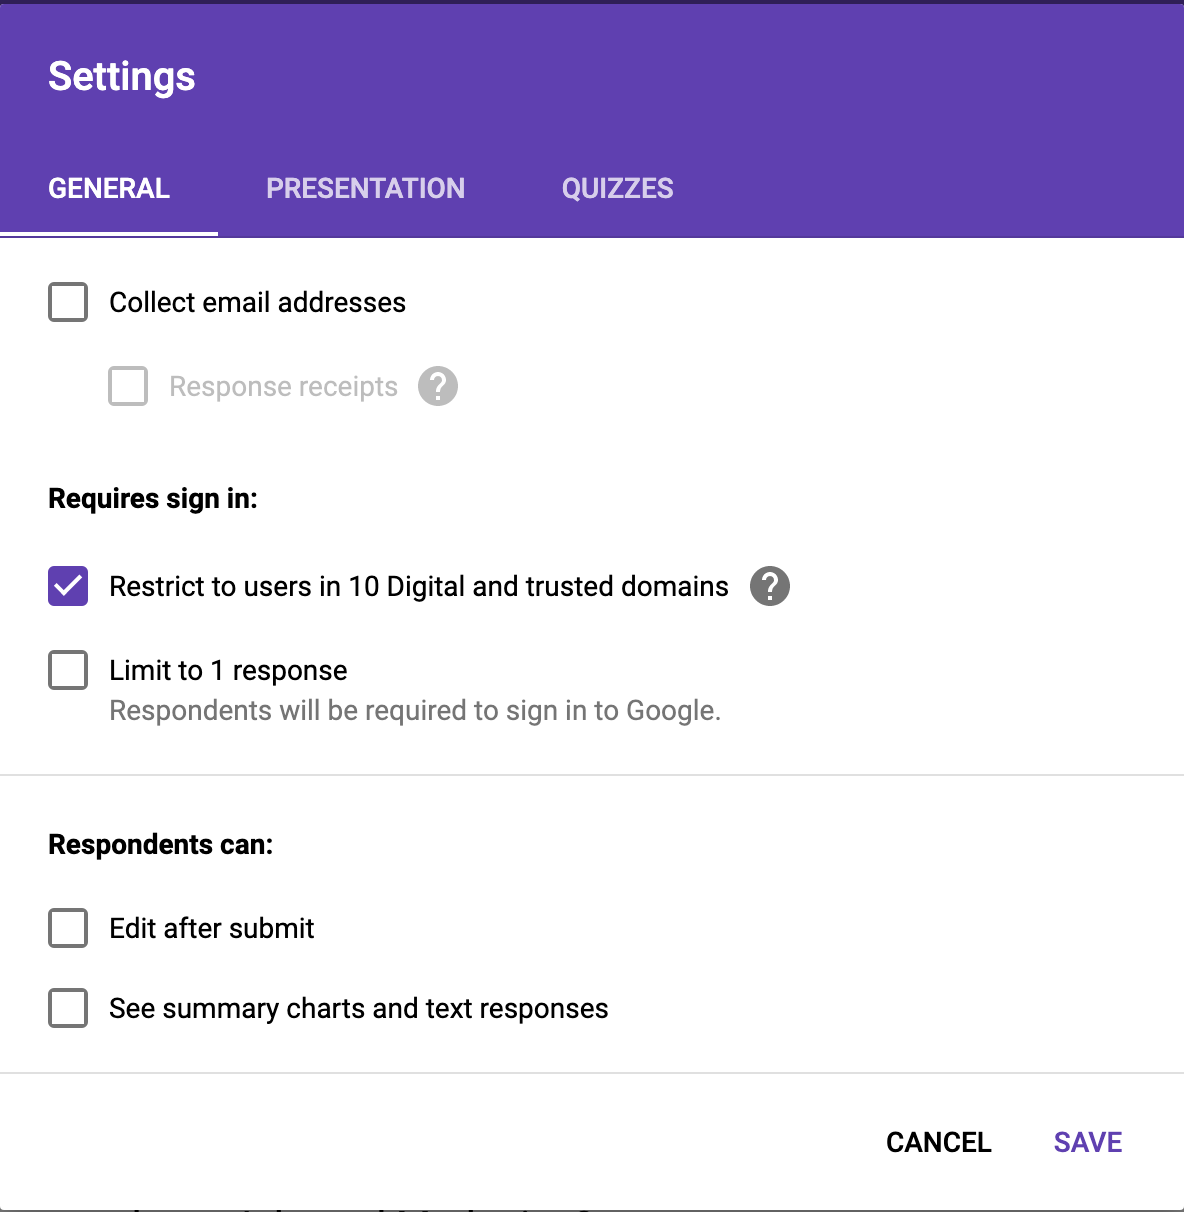
\includegraphics[height=.30\textheight]{img/gf/gf-form-set1}
		\caption{Google Form - Opções}
		\label{fig:gf-form-set1}
	\end{center}
\end{figure}

\begin{figure}[ht!]
	\begin{center}
		\begin{minipage}{0.40\textwidth}
			\begin{center}
				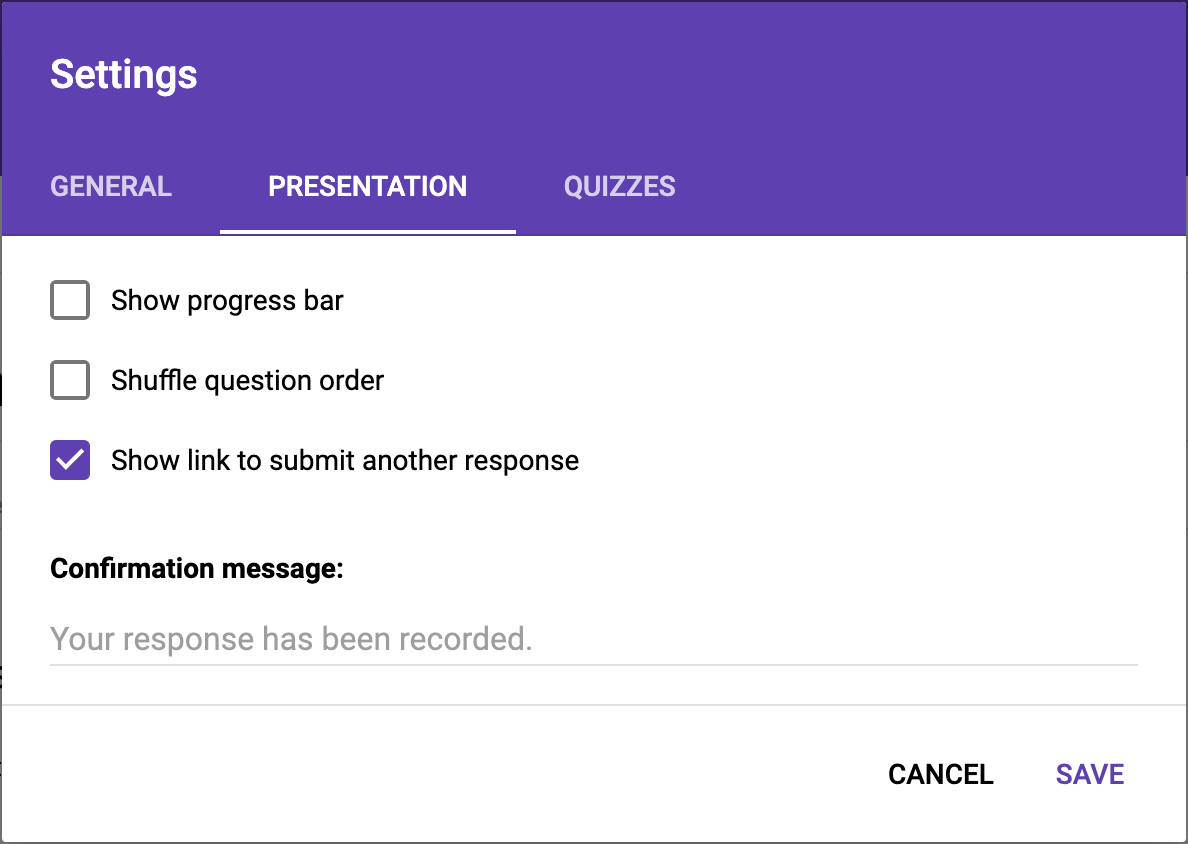
\includegraphics[height=.22\textheight]{img/gf/gf-form-set2}
				\caption{Google Form - Opções}
				\label{fig:gf-form-set2}
			\end{center}
		\end{minipage}
		\hspace{2cm}
		\begin{minipage}{0.40\textwidth}
			\begin{center}
				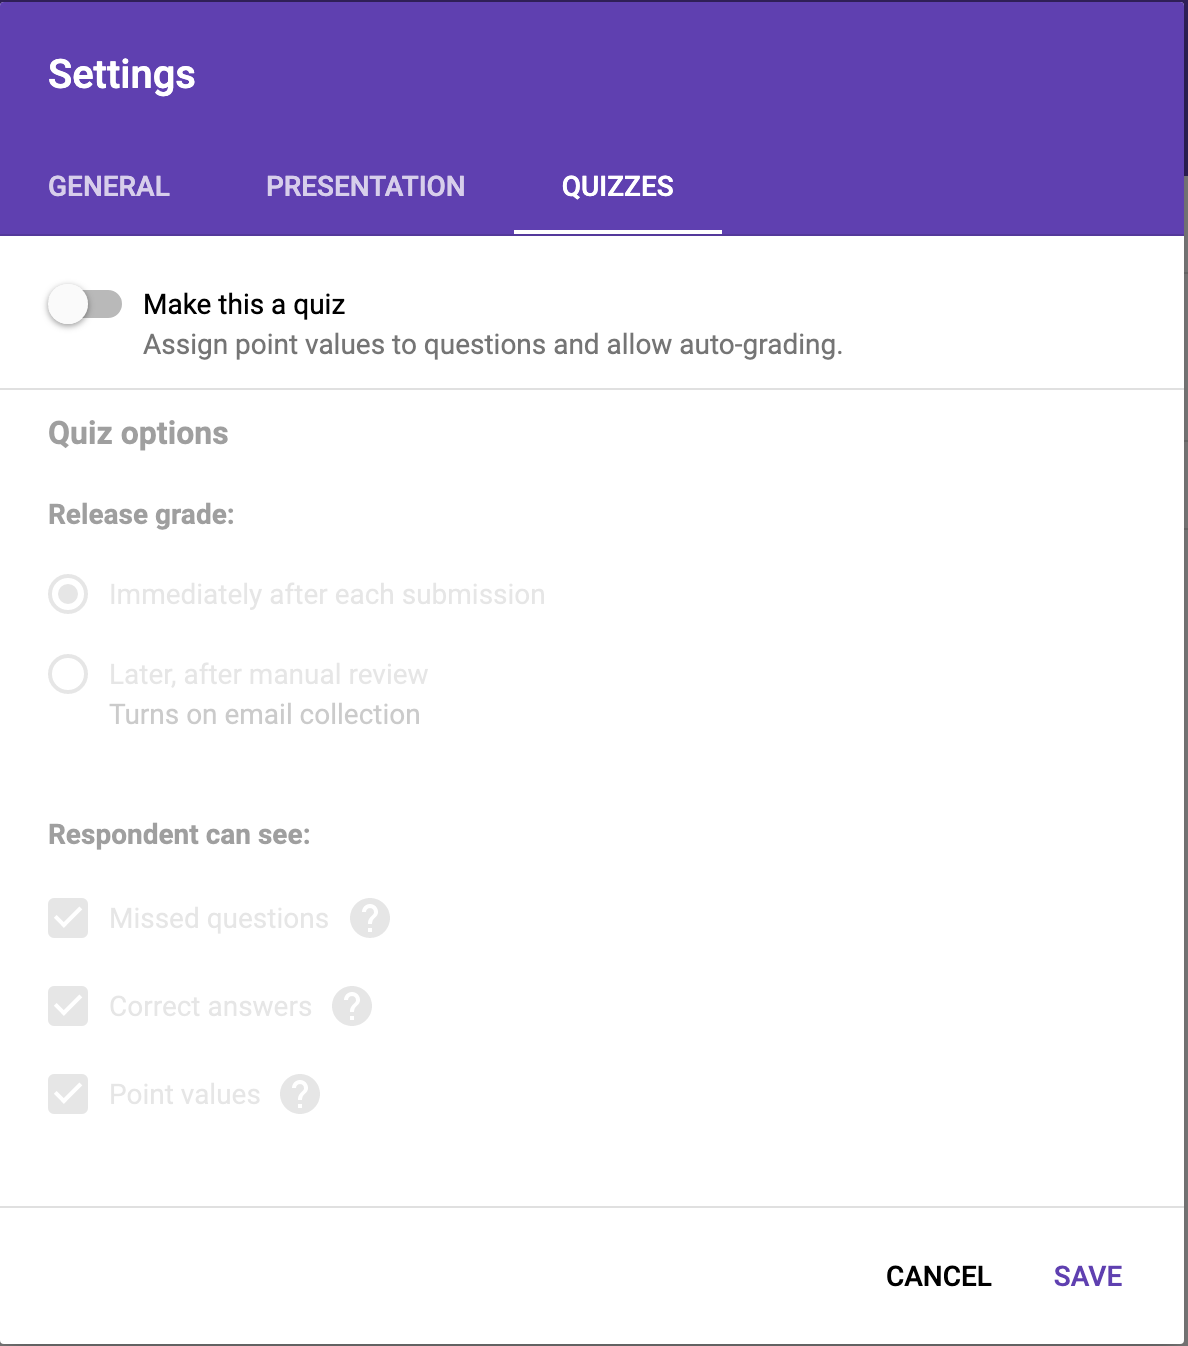
\includegraphics[height=.30\textheight]{img/gf/gf-form-set3}
				\caption{Google Form - Opções}
				\label{fig:gf-form-set3}
			\end{center}
		\end{minipage}
	\end{center}
\end{figure}

Antes de partilhar o formulário, precisamos de verificar se o formulário ficou construido como planeado e para isso a aplicação fornece a funcionalidade: \textit{preview}. O Google Form permite os utilizadores enviarem o formulário através de um link, por email, embebido num pagina web ou partilhando no Facebook ou Tweeter utilizando os botões de partilha rápida.

Na análise de resultados, como podemos ver na Figura \ref{fig:gf-form-results} a aplicação faz uma exibição do resumo das respotas, mostrando alguns gráficos/estatisticas contudo, o utilizador não dispõe de nenhuma funcionalidade que filtra ou segmenta os dados. A unica maneira que o utilizador tem de poder tratar os dados e segmenta-los é, depois de exportar os dados, utilizando o Google Sheets, que já requer algum conhecimento na ferramenta. 


\begin{figure}[ht!]
	\begin{center}
		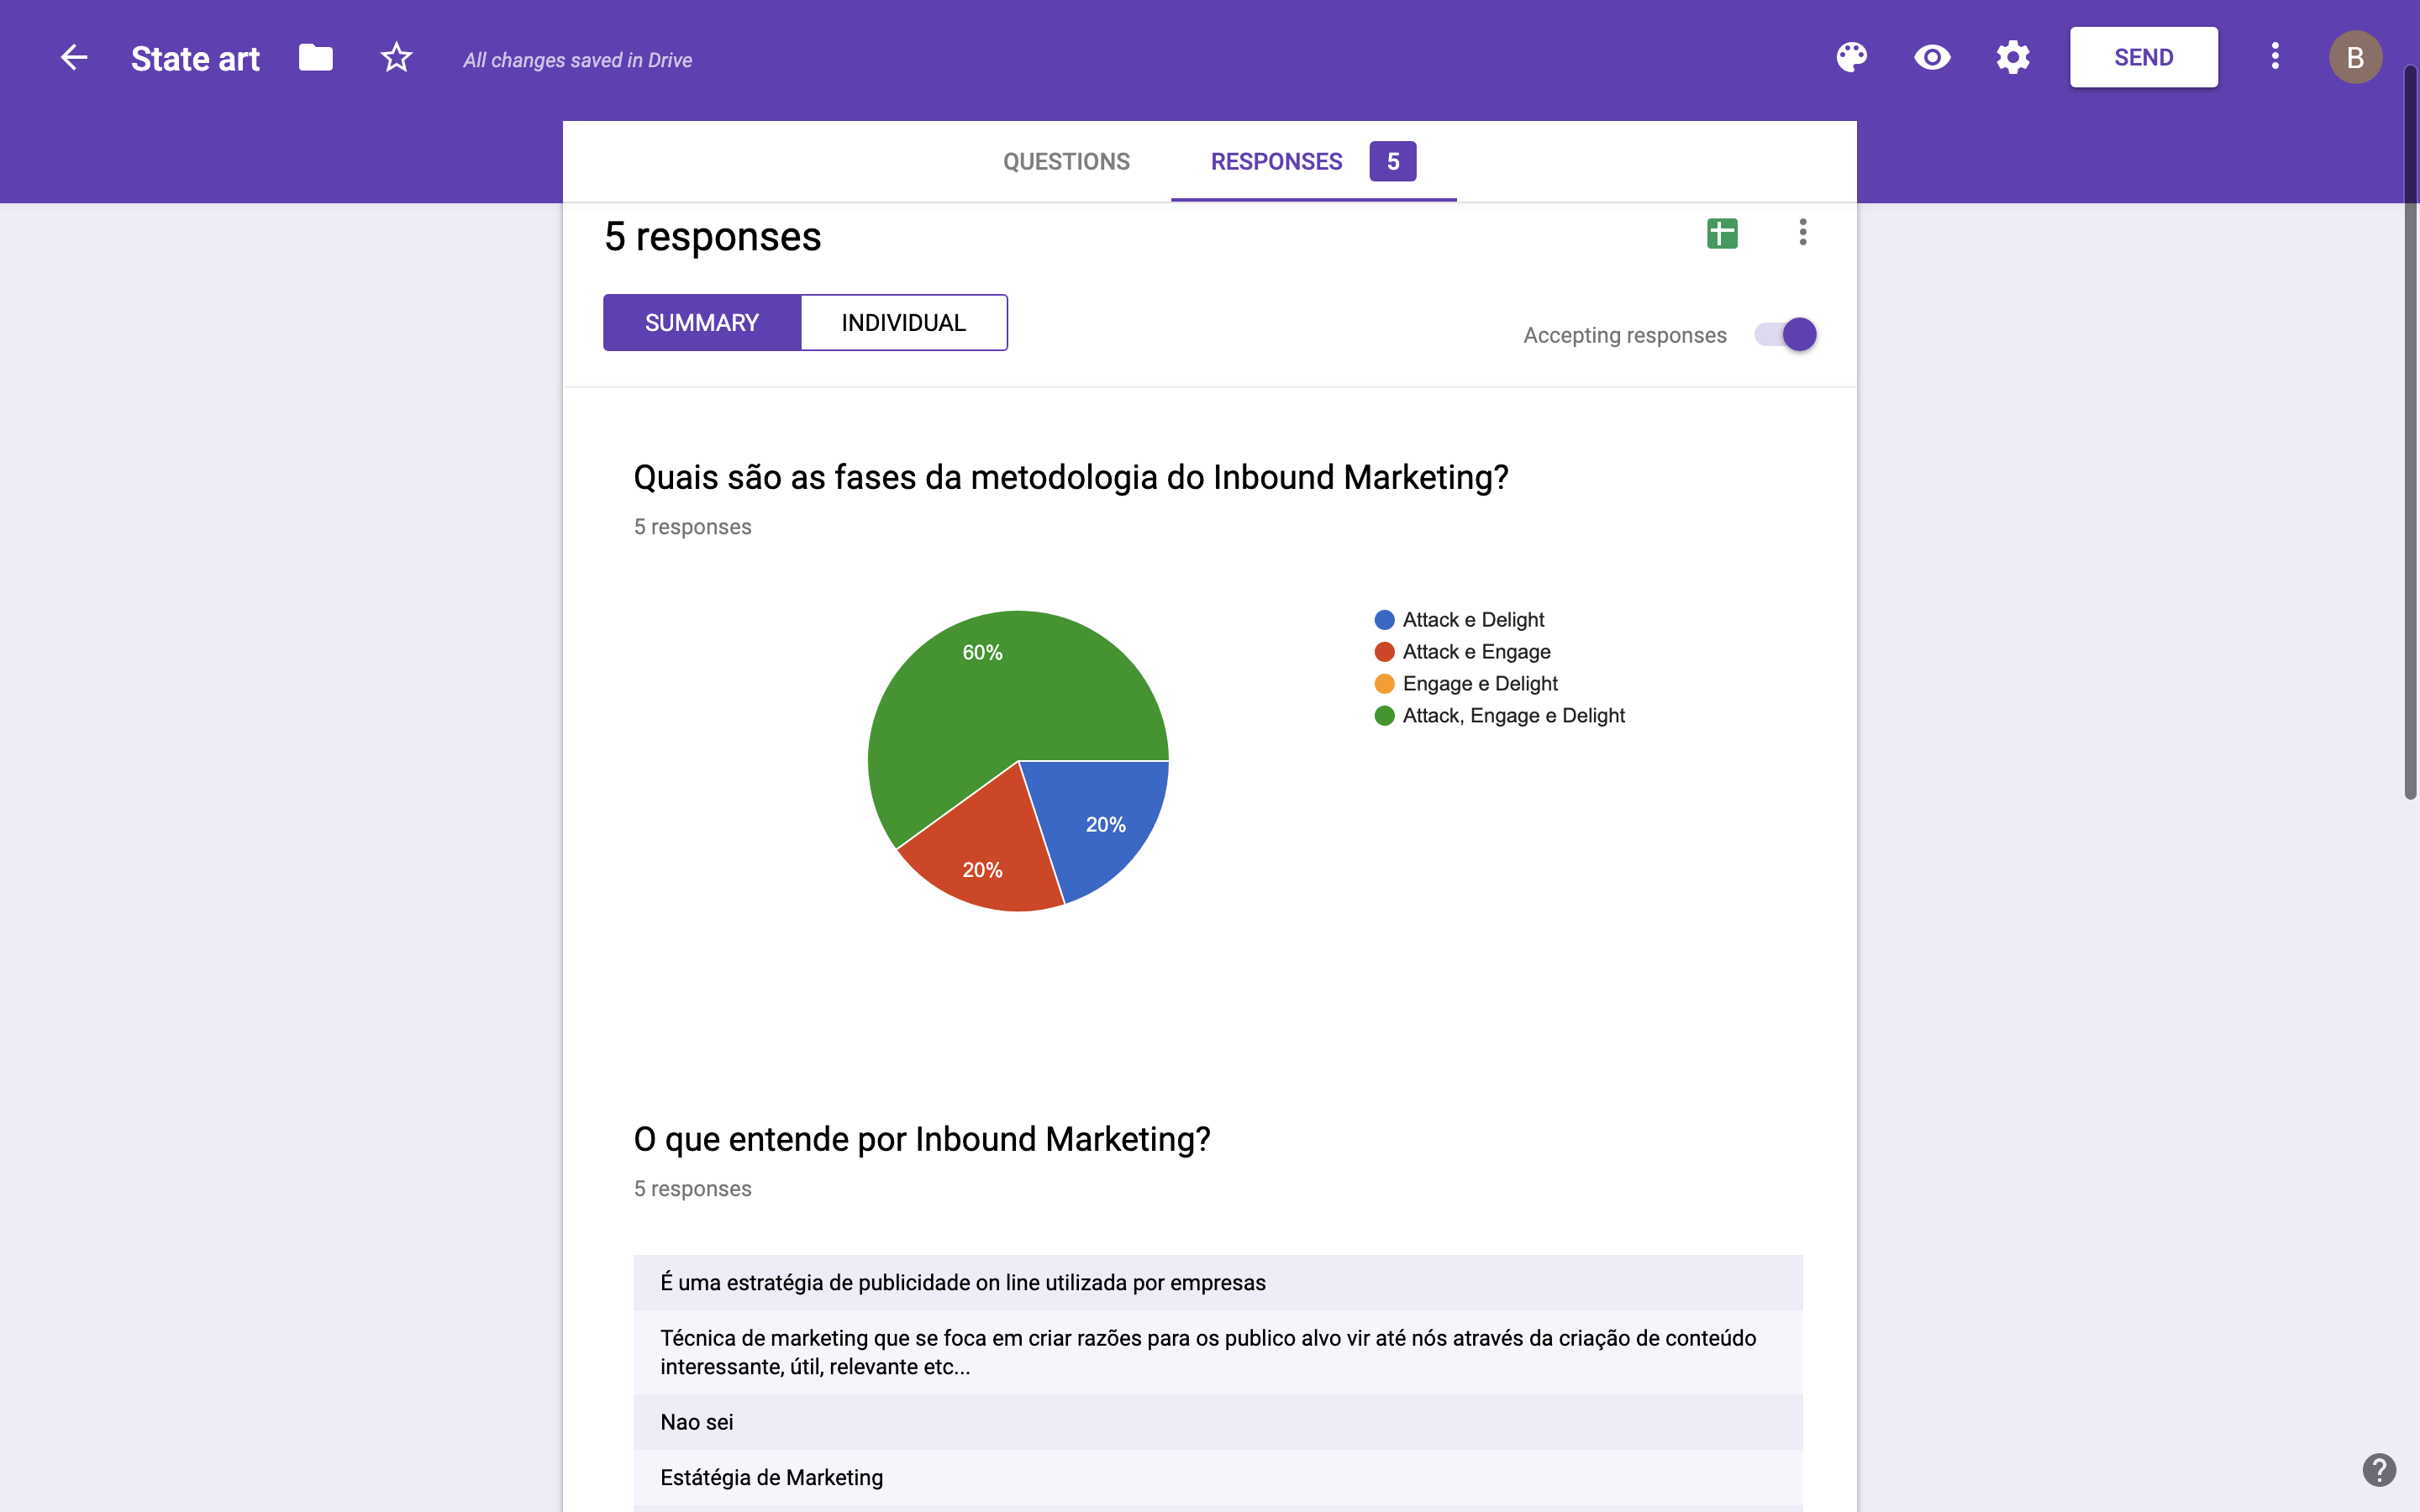
\includegraphics[width=1\textwidth]{img/gf/gf-form-results}
		\caption{Google Form - Sumério dos resultados obtidos}
		\label{fig:gf-form-results}
	\end{center}
\end{figure}

\section{\acrfull{tcg}}

O \acrlong{tcg} é um produto actualmente no mercado, desenvolvido pela equipa da 10.digital, que tem como principal objectivo transformar pdf's numa aprendizagem baseada em tentativa erro. O \acrshort{tcg} nasceu de uma forte convicção de que perder apenas 2 minutos por dia numa formação tentativa erro é uma optima forma de aprender, poupando tempo e dinheiro às empresas. Inicialmente muito focado em formação interna, a equipa do \acrshort{tcg} foi-se apercebendo que existem muitos outros problemas (e. g. Consolidação de procedimentos, \textit{Onboarding} de novos colaboradores, Divulgação da cultura da empresa, Divulgação de informações técnicas a parceiros/clientes ...) para o qual a plataforma tem solução (e. g. Assimilação da cultura de empresa e do espírito das marcas, Simplificação do processo de acolhimento, Redução de custos em reuniões periódicas, Facilidade em divulgar aspectos técnicos, que de outra, forma demorariam mais tempo ...).\cite{tcginfo}

O \acrshort{tcg} é um \acrshort{saas} pago que disponibiliza uma demo de 30 dias. Esta demo permite ao utilizador utilizar todas as funcionalidades da plataforma e, tal como nos planos pagos, disponibiliza ainda um tutorial de como efectuar as actividades chaves.

Este produto permite-nos criar utilizadores finais (i. e. quem irá responder à formação), questões e formaçãos. As questões e os utilizadores finais, são categorizados através de tags, optimizando assim a forma como associamos os mesmos a uma formação nova ou já existente, como veremos em diante.

 Como podemos ver na Figura \ref{fig:tcg-homepage} na página inicial, a plataforma expõem algumas estatísticas gerais sobre as formações do utilizador.
 
 \newpage


\begin{figure}[ht!]
	\begin{center}
		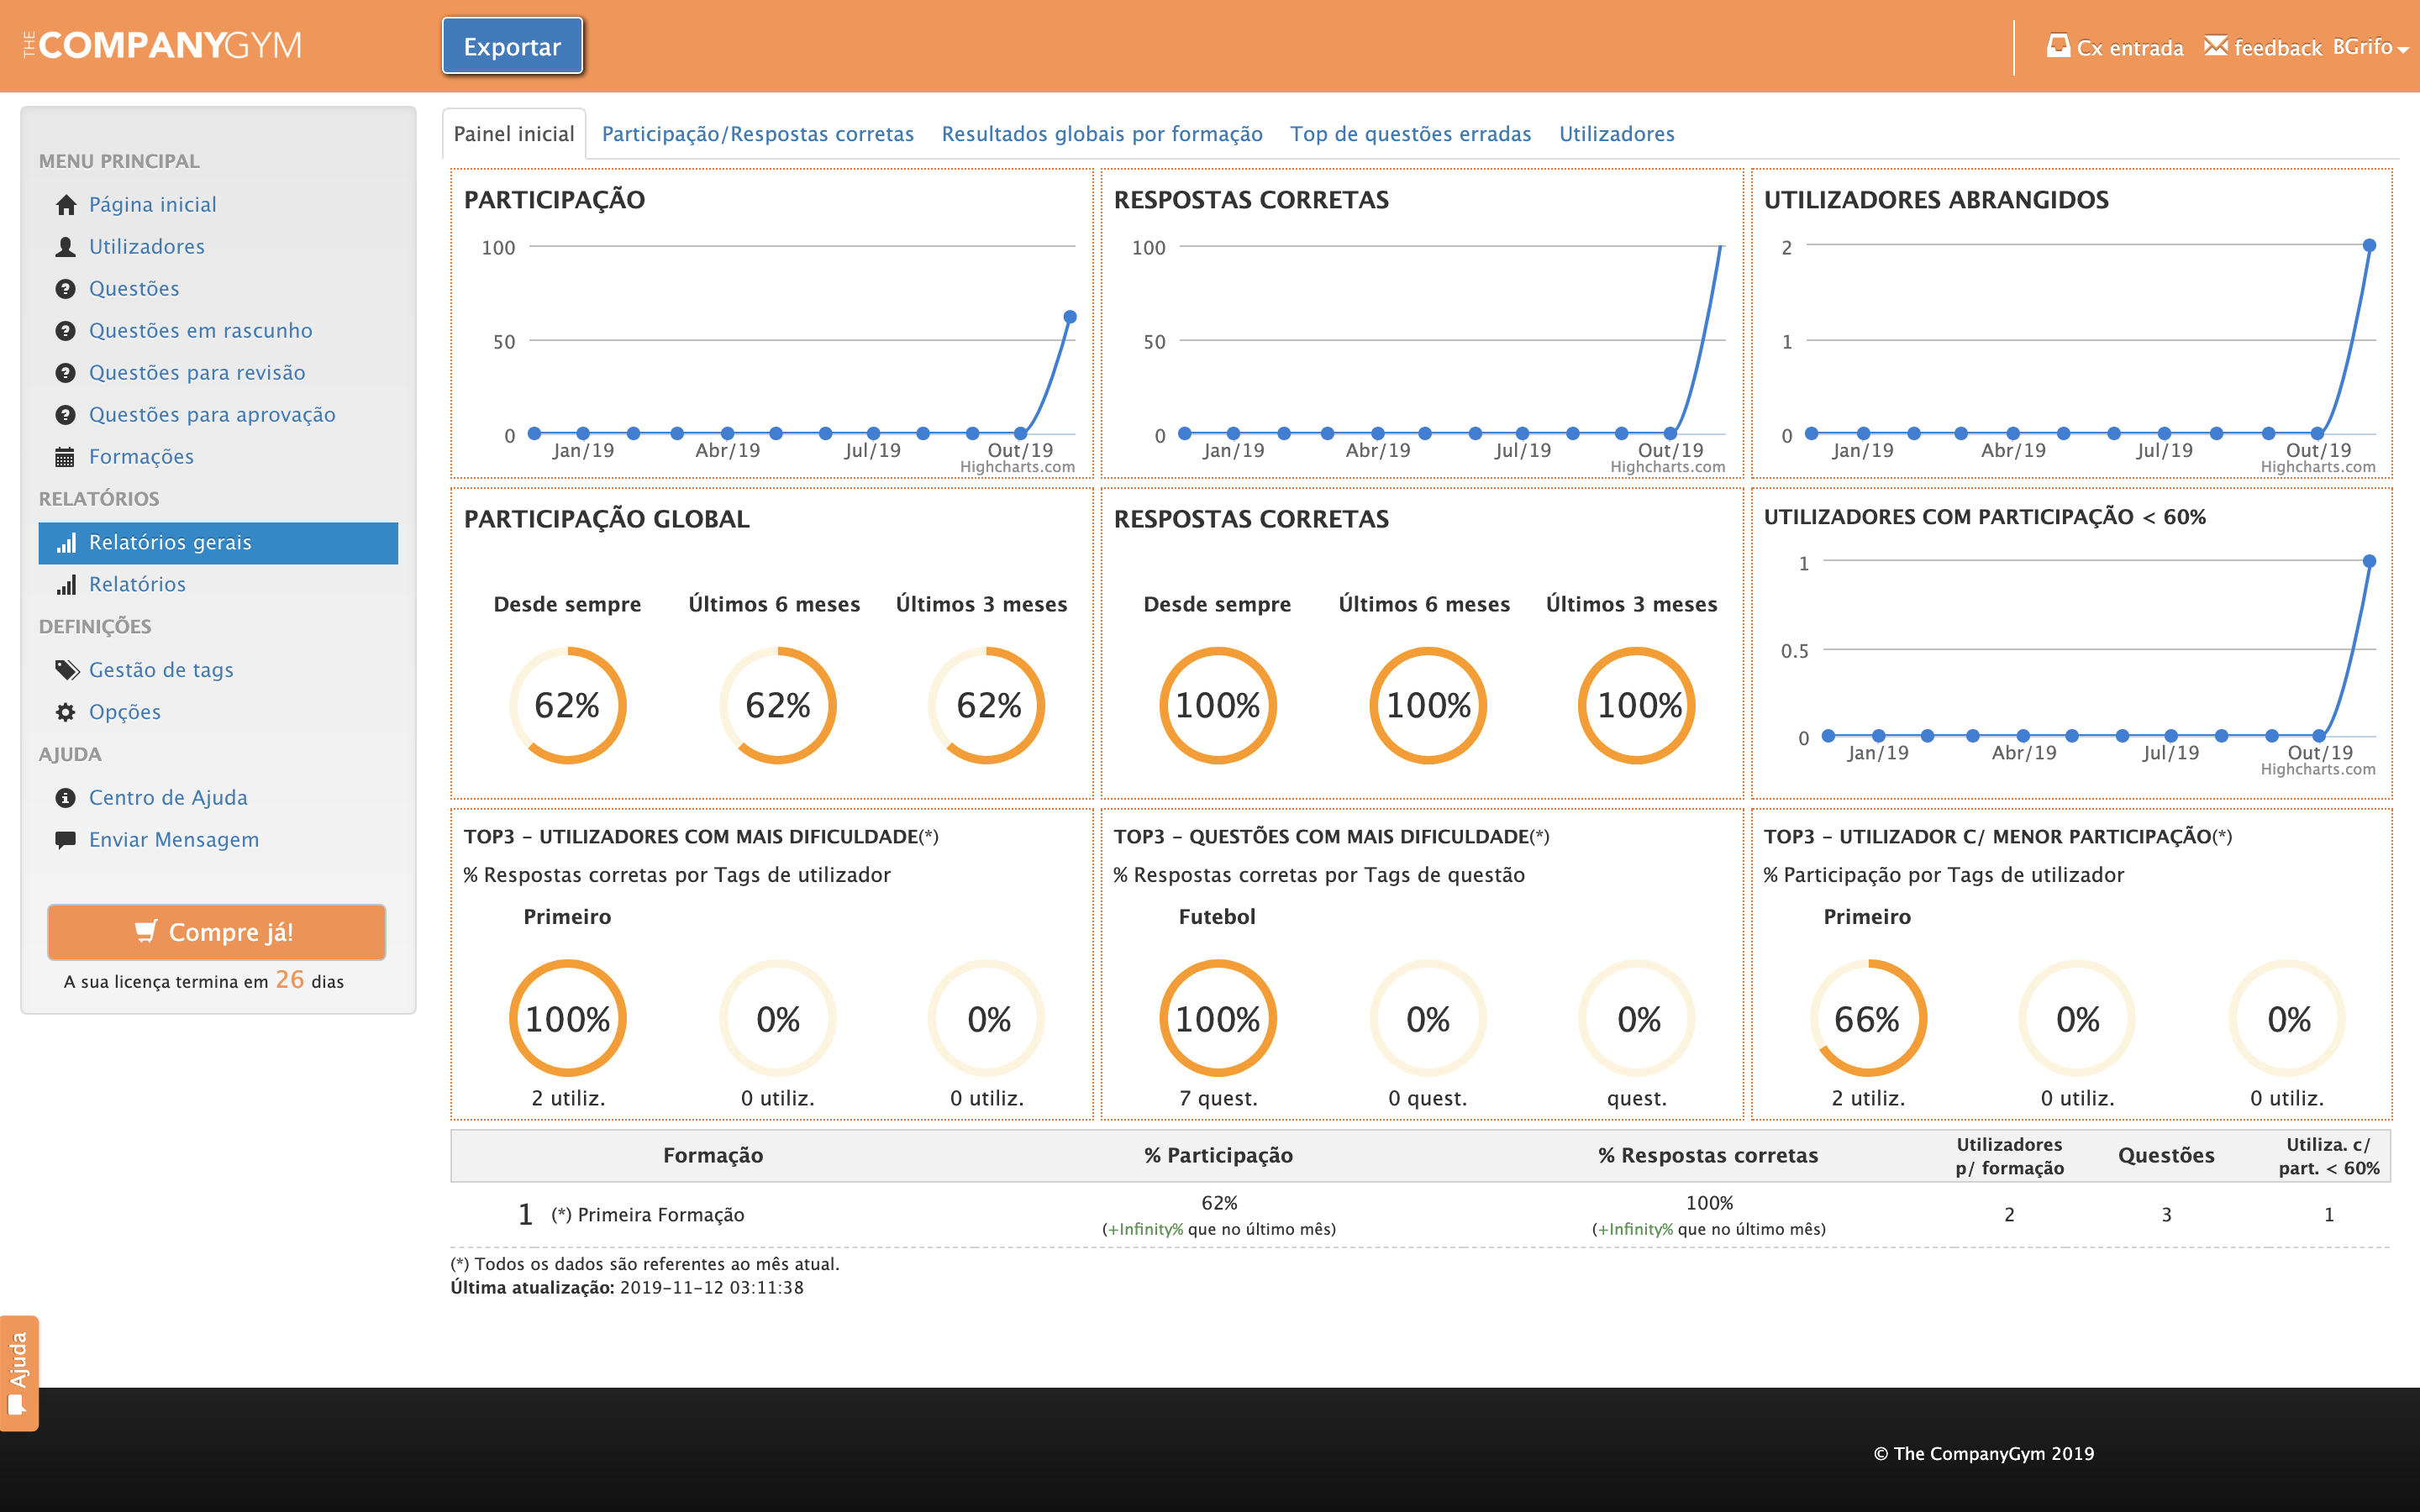
\includegraphics[width=1\textwidth]{img/tcg/tcg-homepage.png}
		\caption{The Company Gym - Página Inicial}
		\label{fig:tcg-homepage}
	\end{center}
\end{figure}

\begin{figure}[ht!]
	\begin{center}
		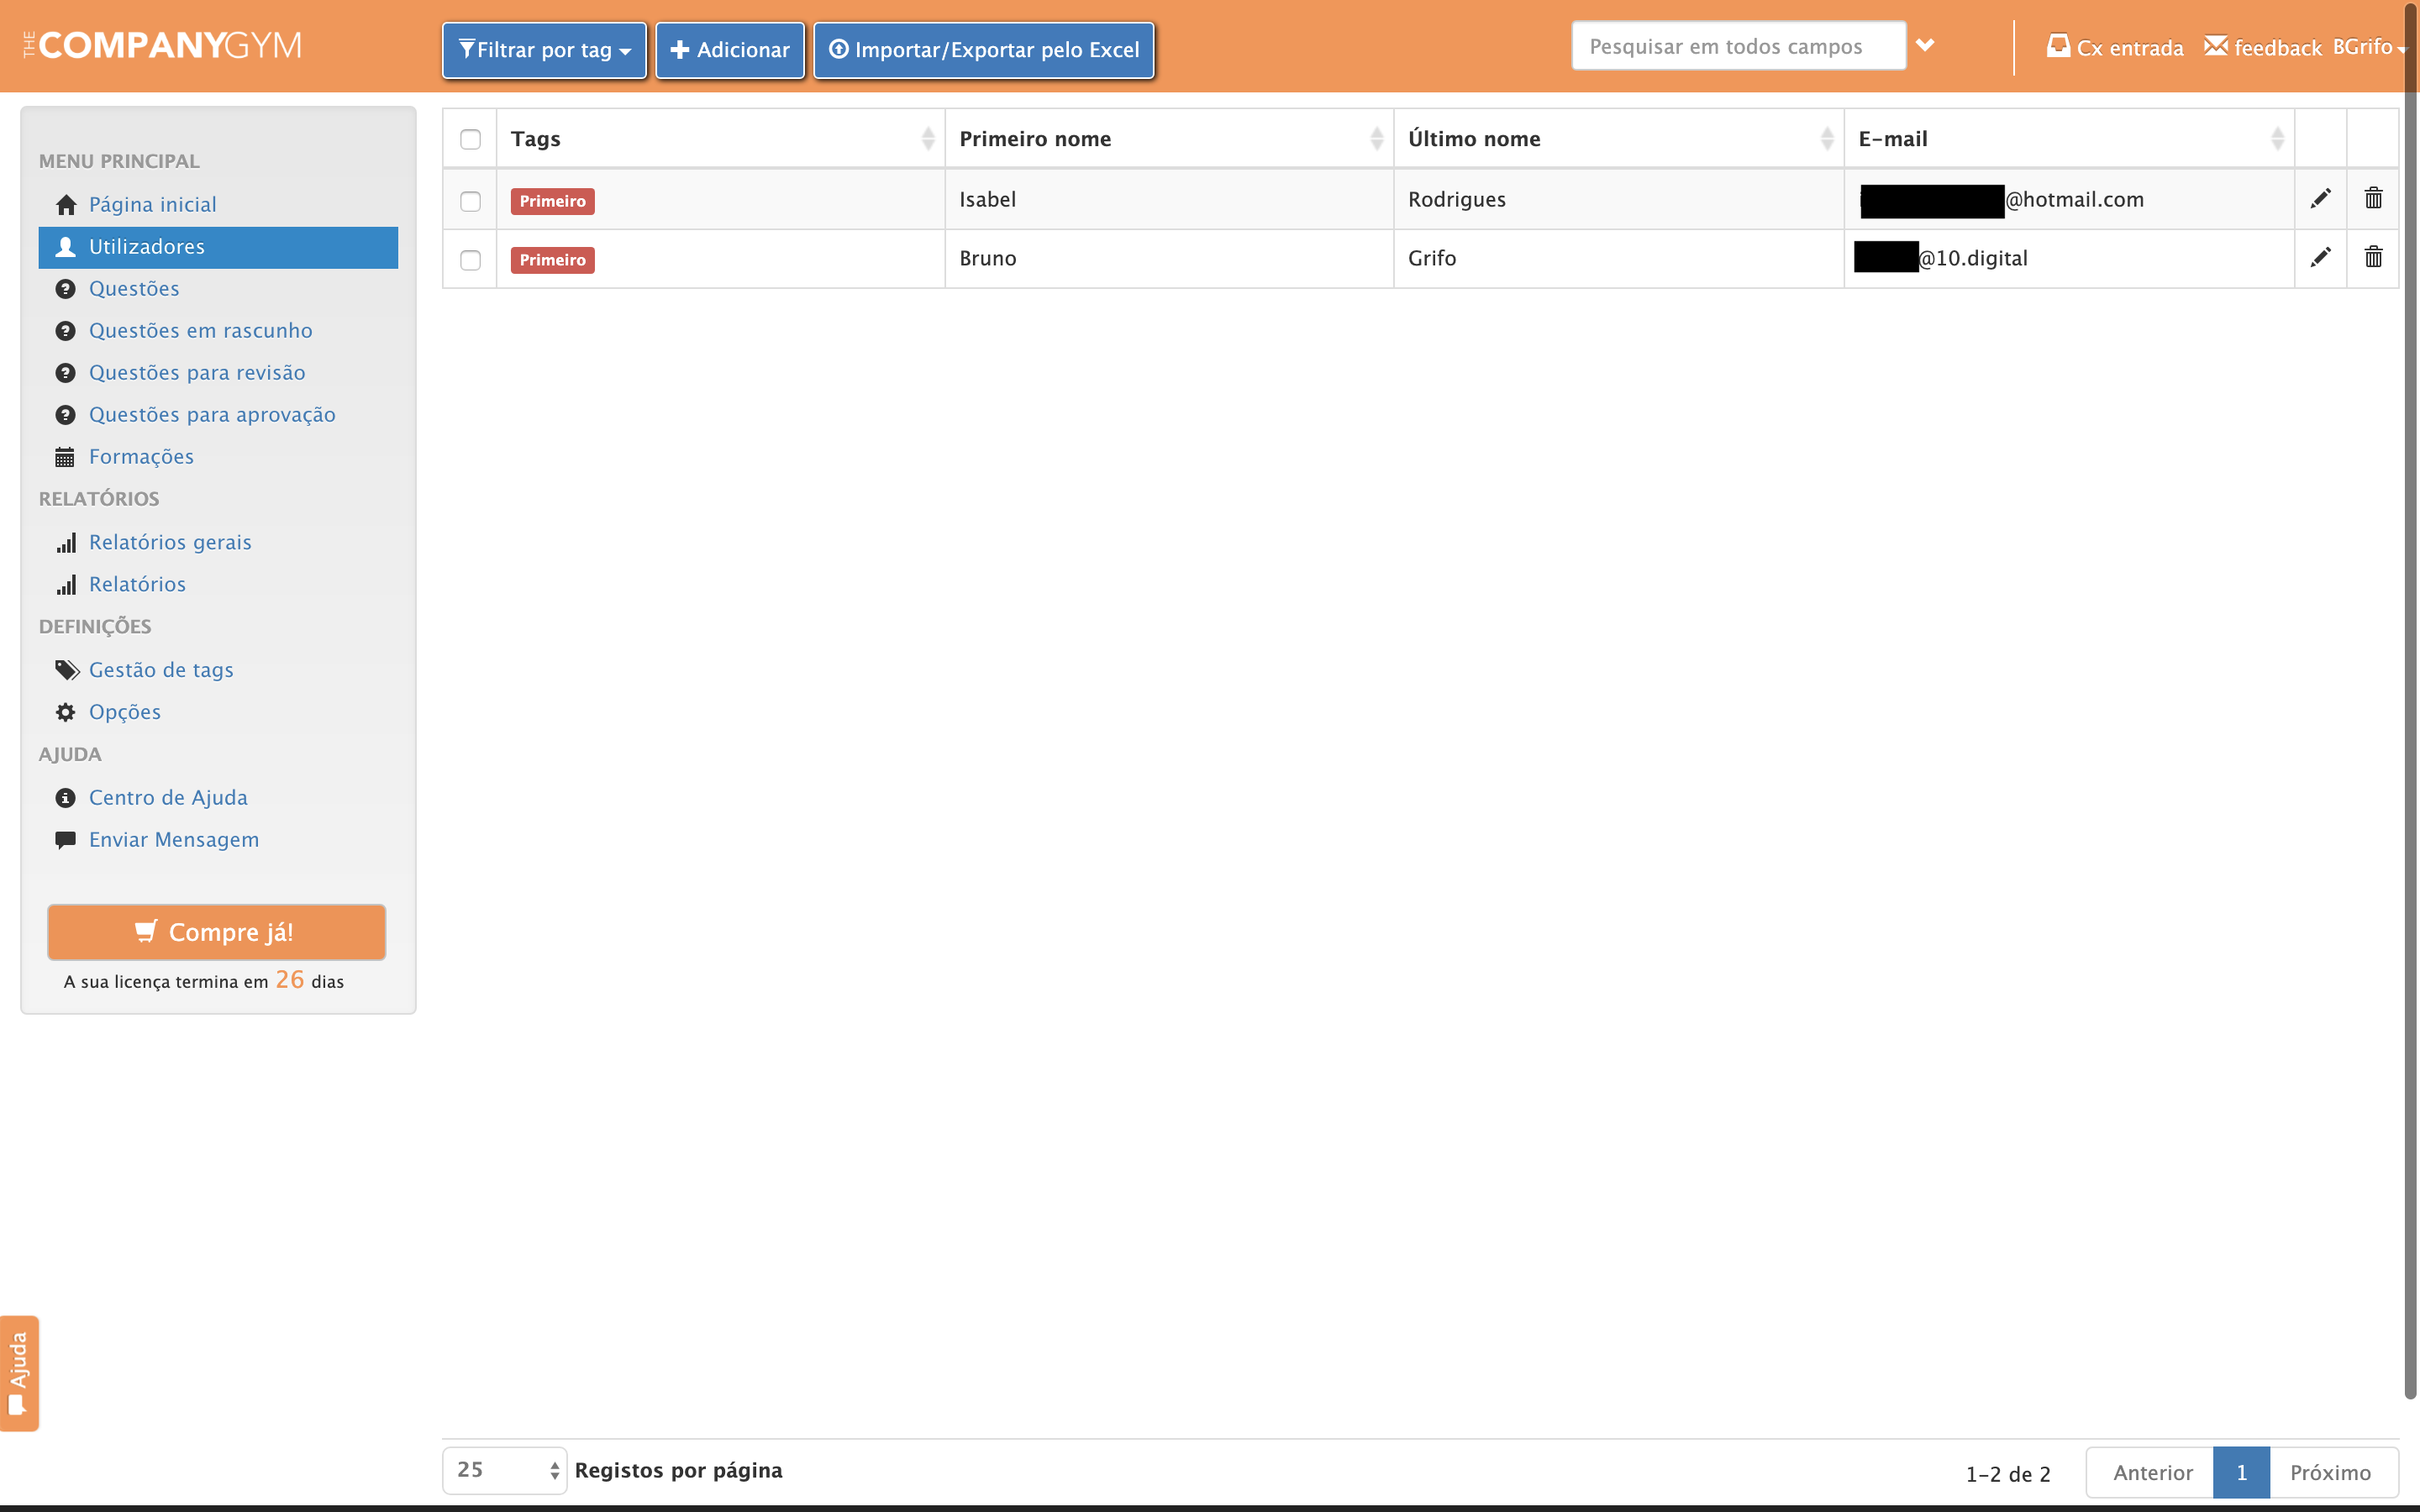
\includegraphics[width=1\textwidth]{img/tcg/tcg-utilizadores.png}
		\caption{The Company Gym - Lista de utilizadores finais}
		\label{fig:tcg-utilizadores}
	\end{center}
\end{figure}

Representado na Figura \ref{fig:tcg-utilizadores} está a lista de utilizadores finais. Para criar um novo utilizador final basta criar no botão "+Adicionar" e introduzir uma(s) tag, nova ou já existente, primeiro e ultimo nome e o e-mail por onde vai receber as formações. Como podemos ver há também um botão que permite importar uma lista de utilizadores finais e exportar a lista de utilizadores finais já adicionados no sistema, numa \textit{spreadsheet}.
\newpage

\begin{figure}[ht!]
	\begin{center}
		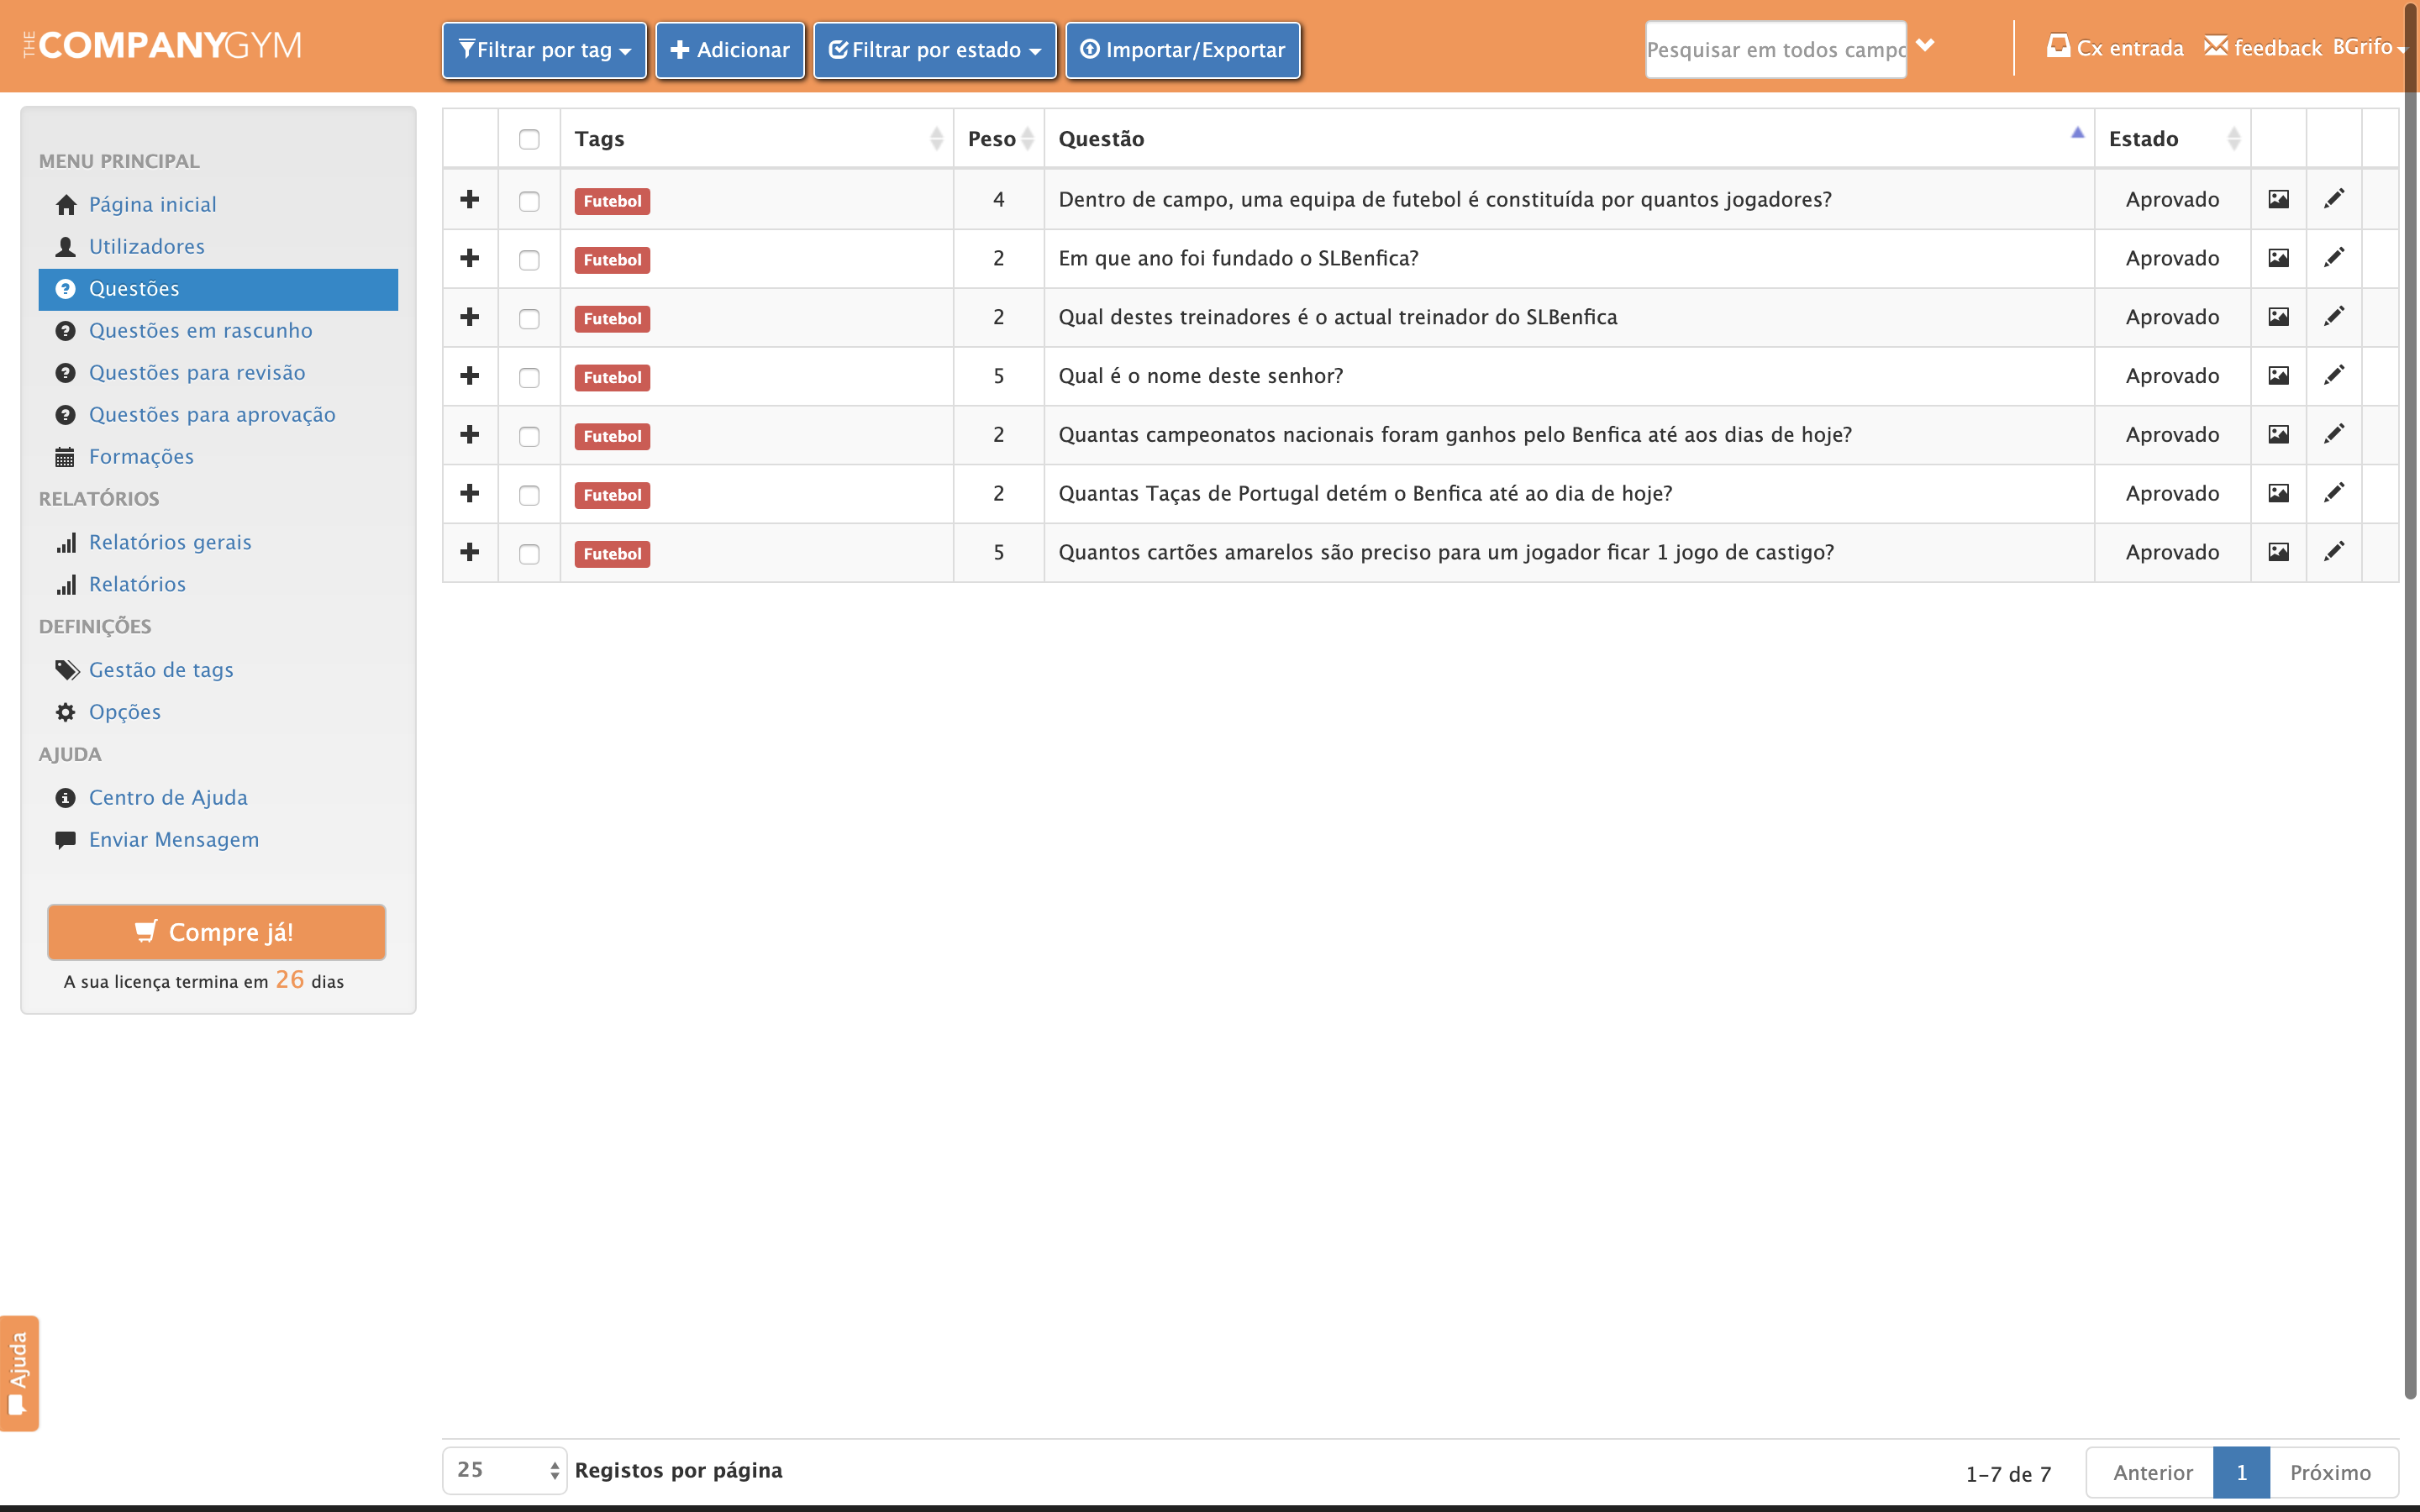
\includegraphics[width=1\textwidth]{img/tcg/tcg-questoes.png}
		\caption{The Company Gym - Lista de questões criadas}
		\label{fig:tcg-questoes}
	\end{center}
\end{figure}

\begin{figure}[ht!]
	\begin{center}
		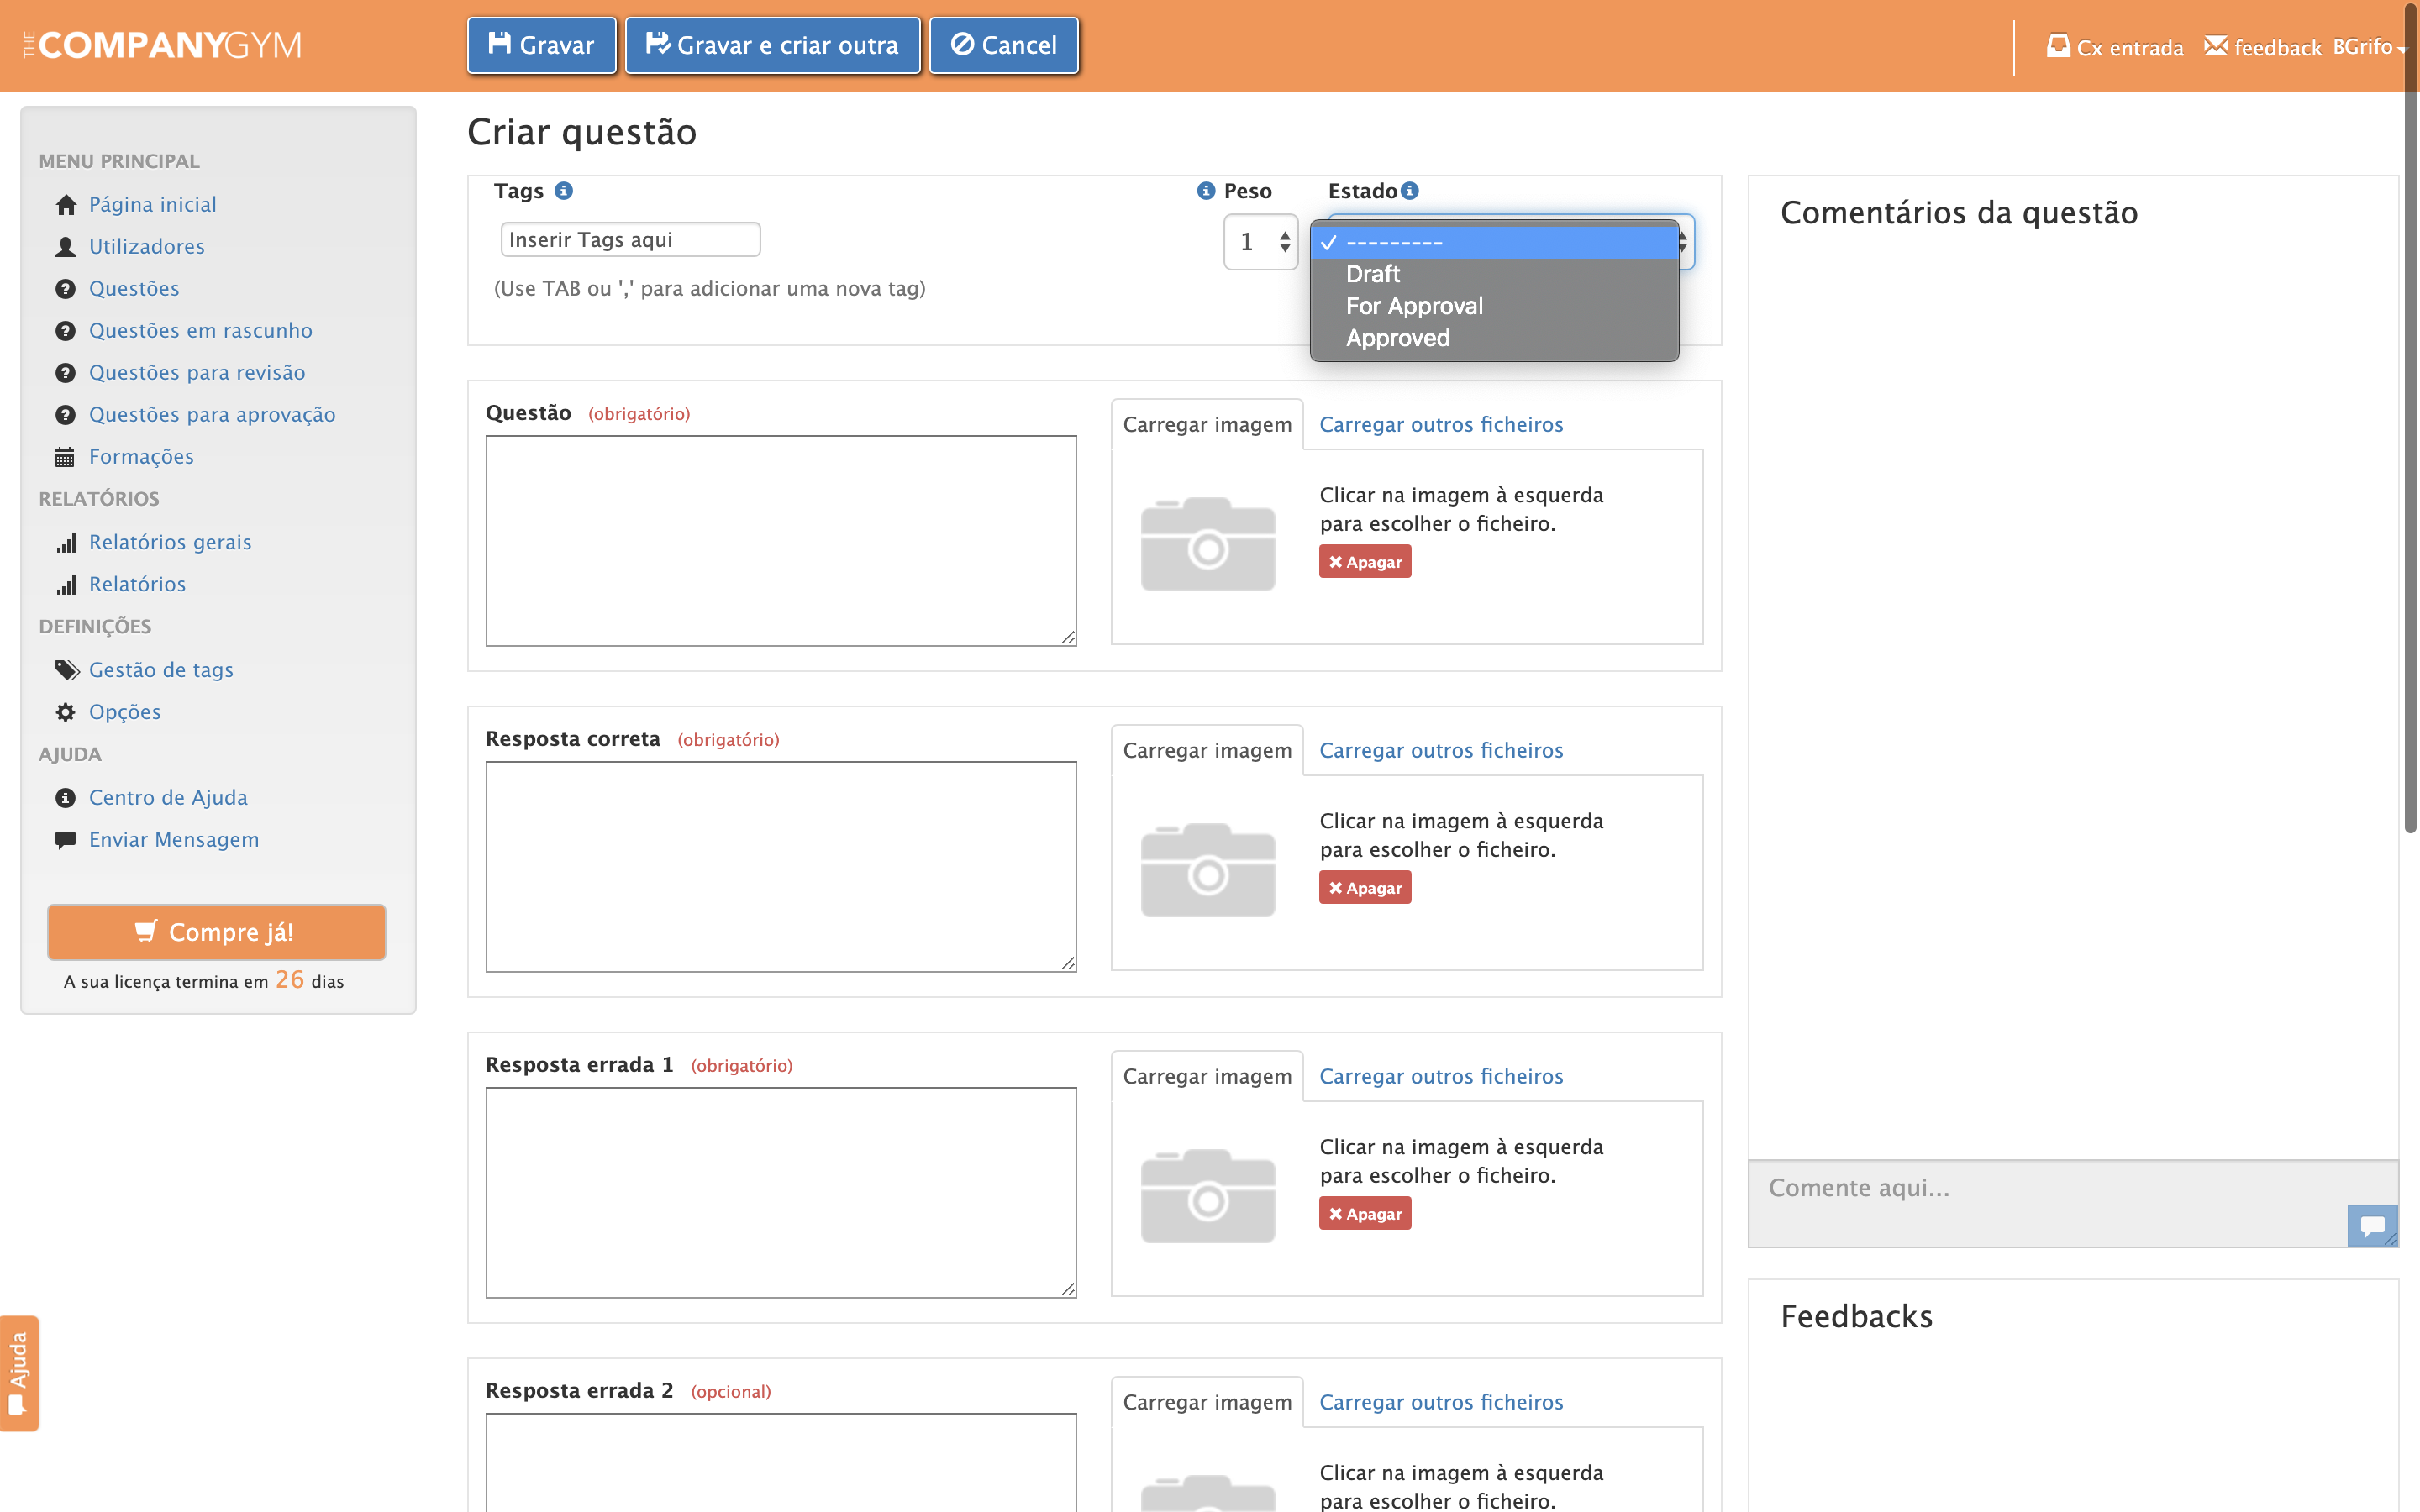
\includegraphics[width=1\textwidth]{img/tcg/tcg-criar-questao.png}
		\caption{The Company Gym - Criar questão}
		\label{fig:tcg-criar-questoes}
	\end{center}
\end{figure}

Na Figura \ref{fig:tcg-questoes} podemos ver que é possível listar todas as questão e filtra-las por \textit{tags} e estado. À semelhança do que acontece com os utilizadores, é também possível importar e exportar questões. Como podemos ver na Figura \ref{fig:tcg-criar-questoes} para criar uma nova questão é necessário atribuir uma(s) \textit{tag}, um peso (i. e. importância), um estado (\textit{draft}, \textit{for aproval} e \textit{aproved}), a questão e pelo menos duas respostas. Alguns alpectos como o anexo (i. e. imagem, video ou fichiero de som) na pergunta e/ou resposta são opcionais. Quando se importa uma serie de pergunas através de uma \textit{spreadsheet} todas as perguntas automaticamente ficam com estado \textit{draft} e como é de esperar sem anexos. Todas as questões que ficam em estado \textit{for aproval} terão de ser aprovadas pelo gestor de conta.


Nas Figuras \ref{fig:tcg-form}, \ref{fig:tcg-form1} e \ref{fig:tcg-form2} temos todas as fases para a criação de uma formação. Em primeiro lugar, é necessário definir a periocidade da formação.  Depois de escolher o nome é necessário dar um dia para o inicio e o fim da mesma, escolher os dias da semana em que o utilizador final irá receber a formação, a hora do dia a que recebe o mail e a duração (i. e. validade) que o utilizador tem para realizar a formação antes da mesma expirar. É de notar que a o sistema aceita uma duração com um max de horas igual à menor diferença entre os dias da semana escolhidos.

 A seleção dos utilizadores finais e das questões faz-se através de tags. Desta forma temos uma forma bastante poderosa de adicionar multiplas perguntas e ao mesmo tempo escolher exatamente quais as perguntas que queremos numa formação e sem ter que fazer quaqueis alterações, adicionar e remover questões a qualquer hora. O mesmo se trata para os utilizadores finais.

\begin{figure}[ht!]
	\begin{center}
		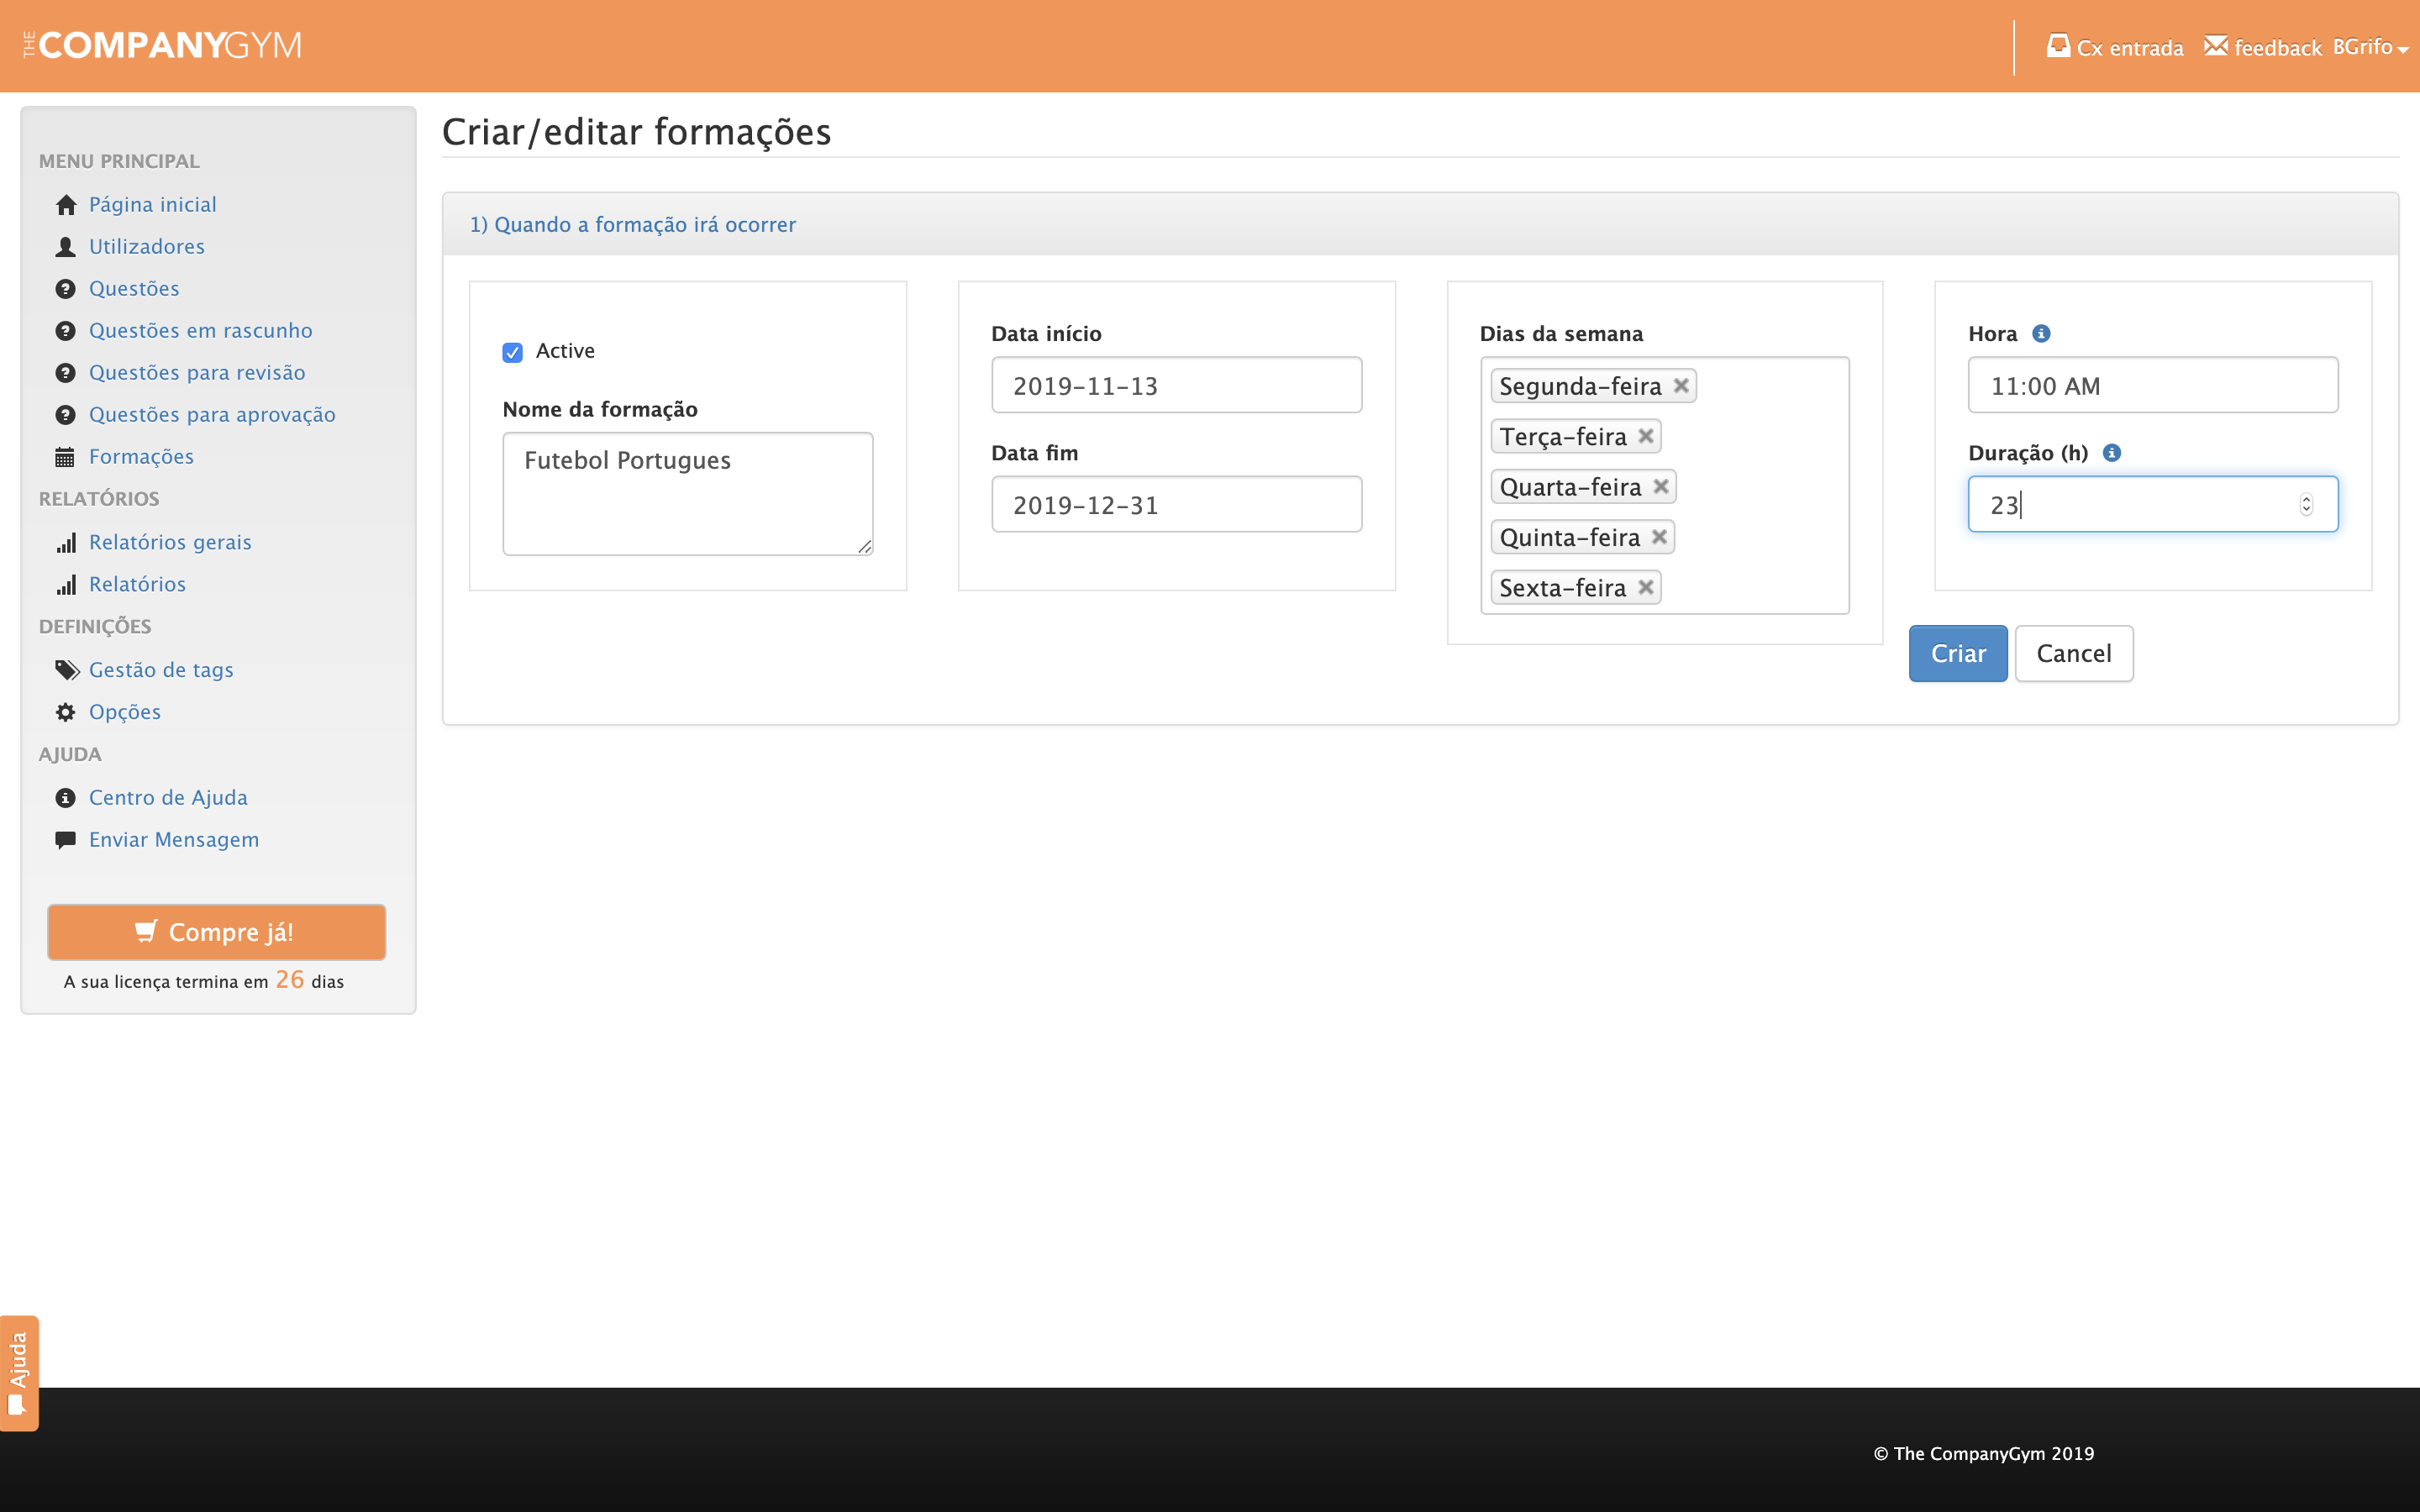
\includegraphics[width=1\textwidth]{img/tcg/tcg-form.png}
		\caption{The Company Gym - Criar Formação (Periodicidade)}
		\label{fig:tcg-form}
	\end{center}
\end{figure}

\begin{figure}[ht!]
	\begin{center}
		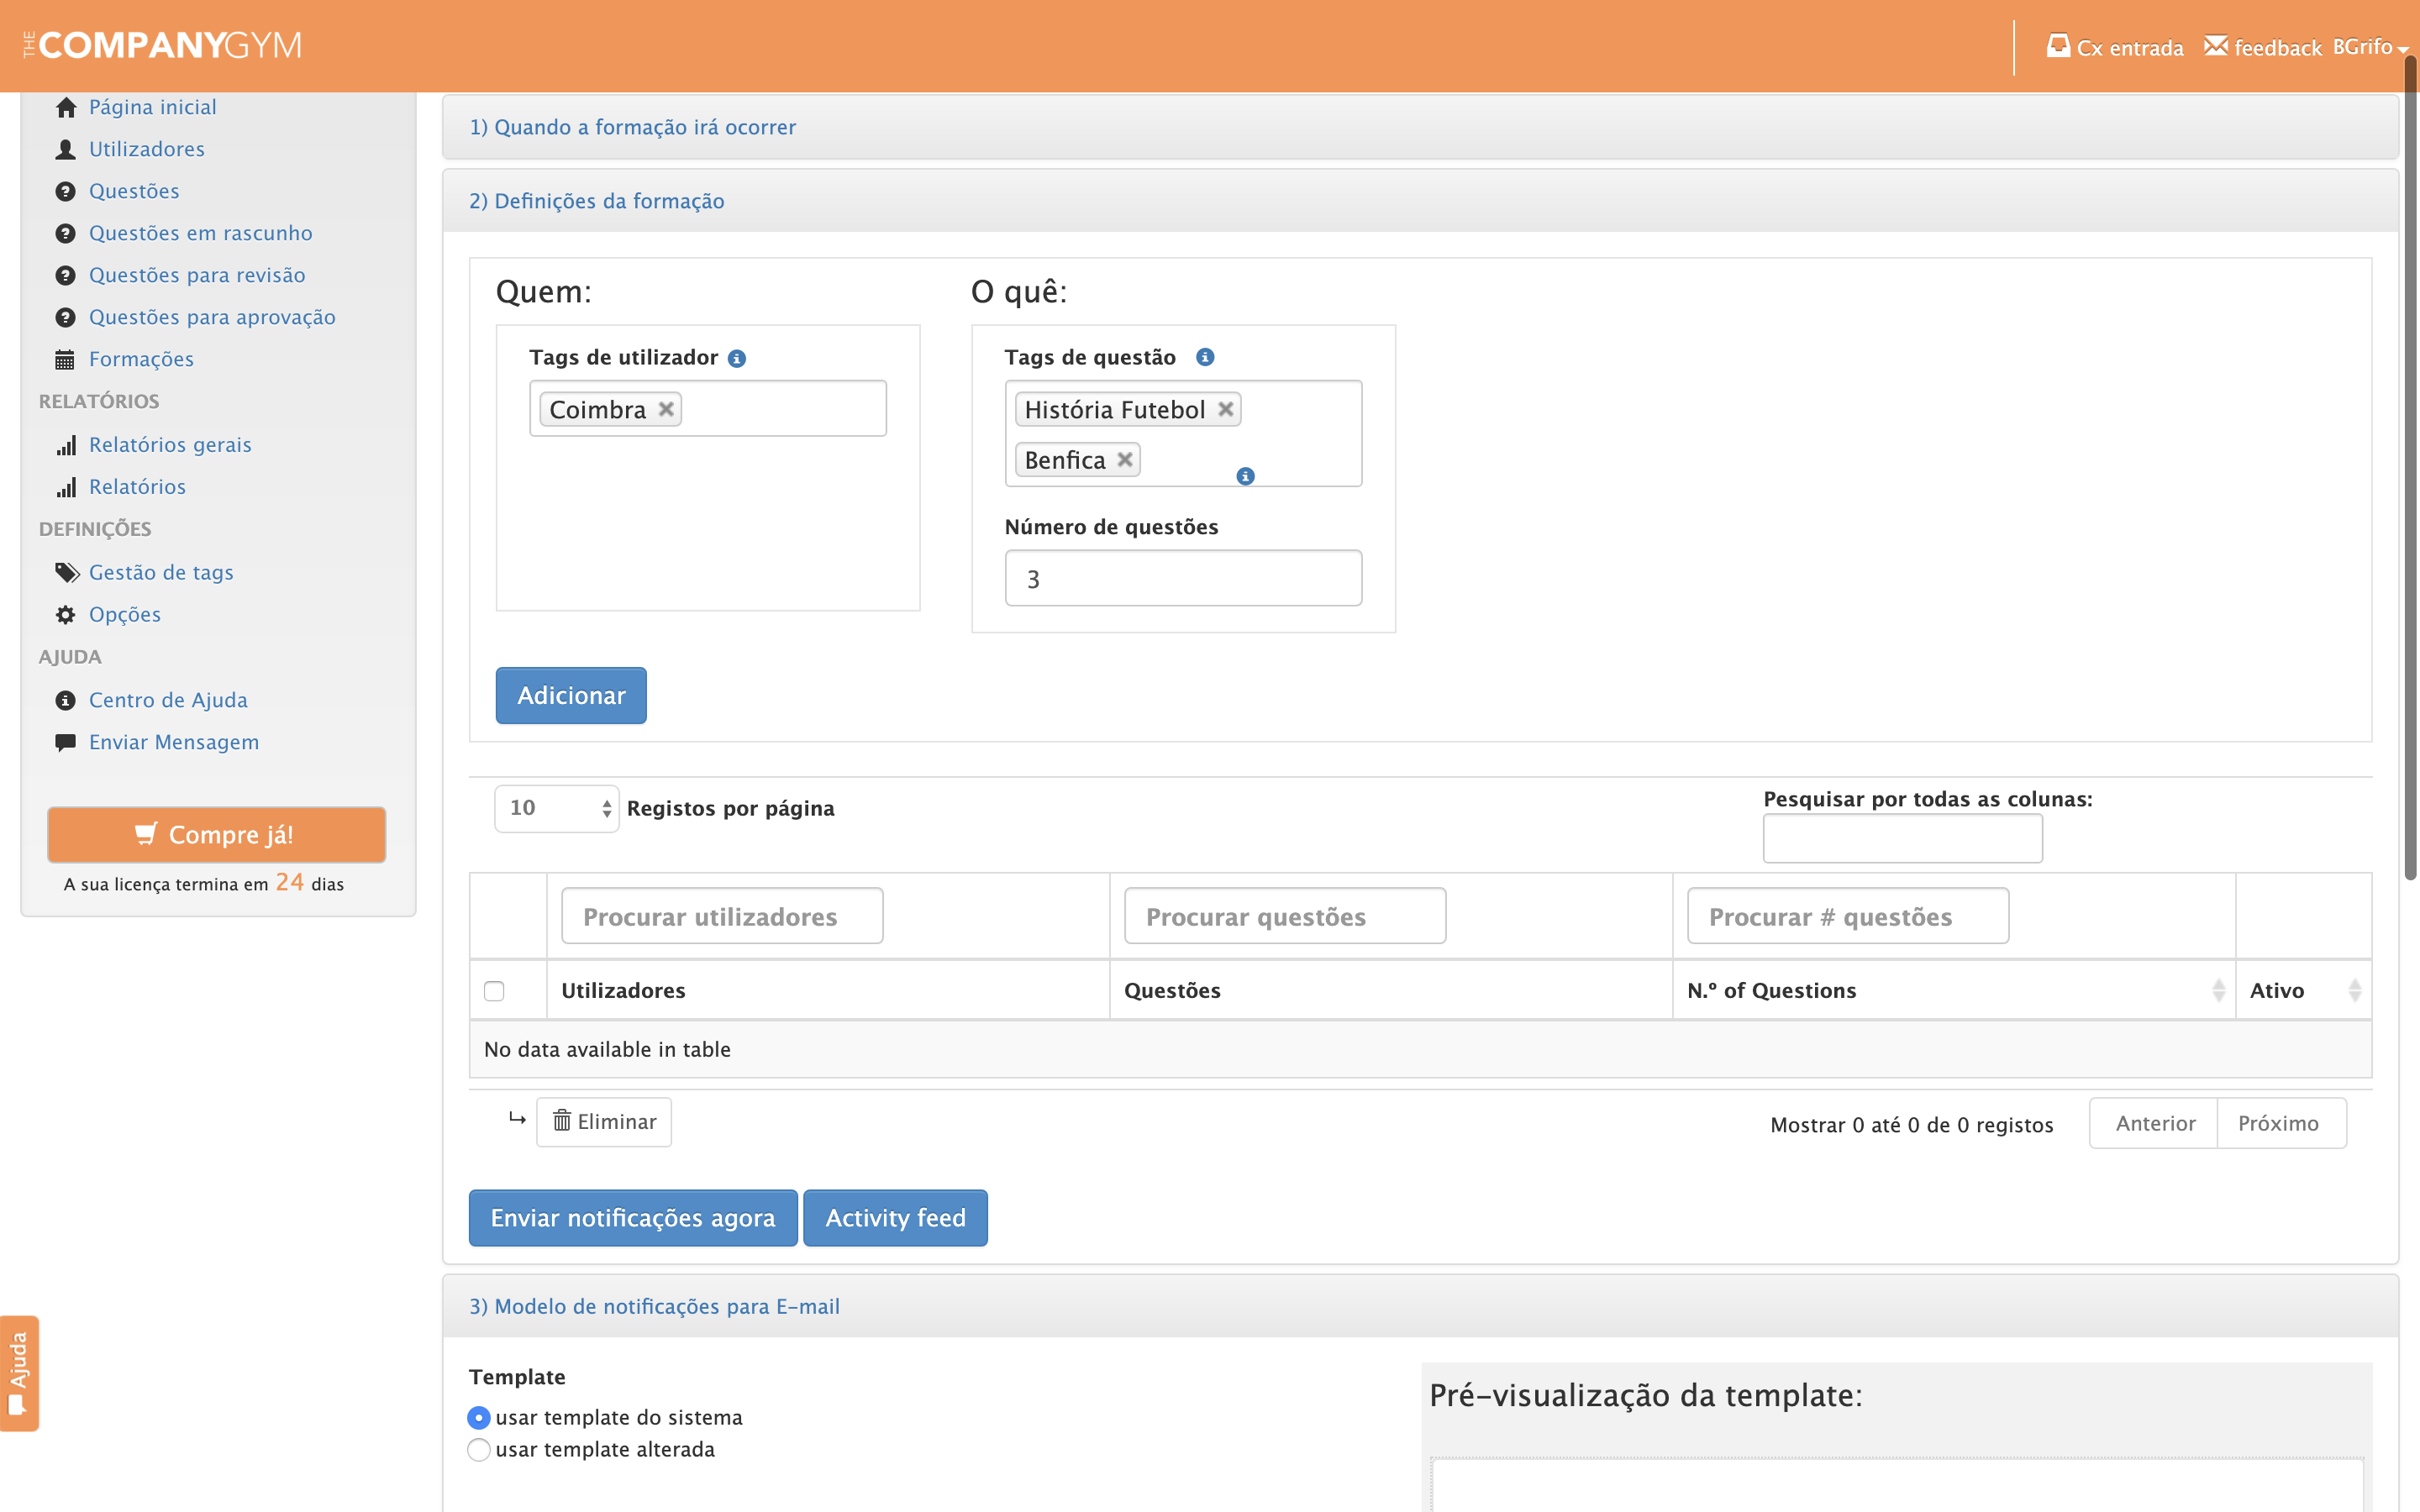
\includegraphics[width=1\textwidth]{img/tcg/tcg-form1.png}
		\caption{The Company Gym - Criar Formação (Definições)}
		\label{fig:tcg-form1}
	\end{center}
\end{figure}

\begin{figure}[ht!]
	\begin{center}
		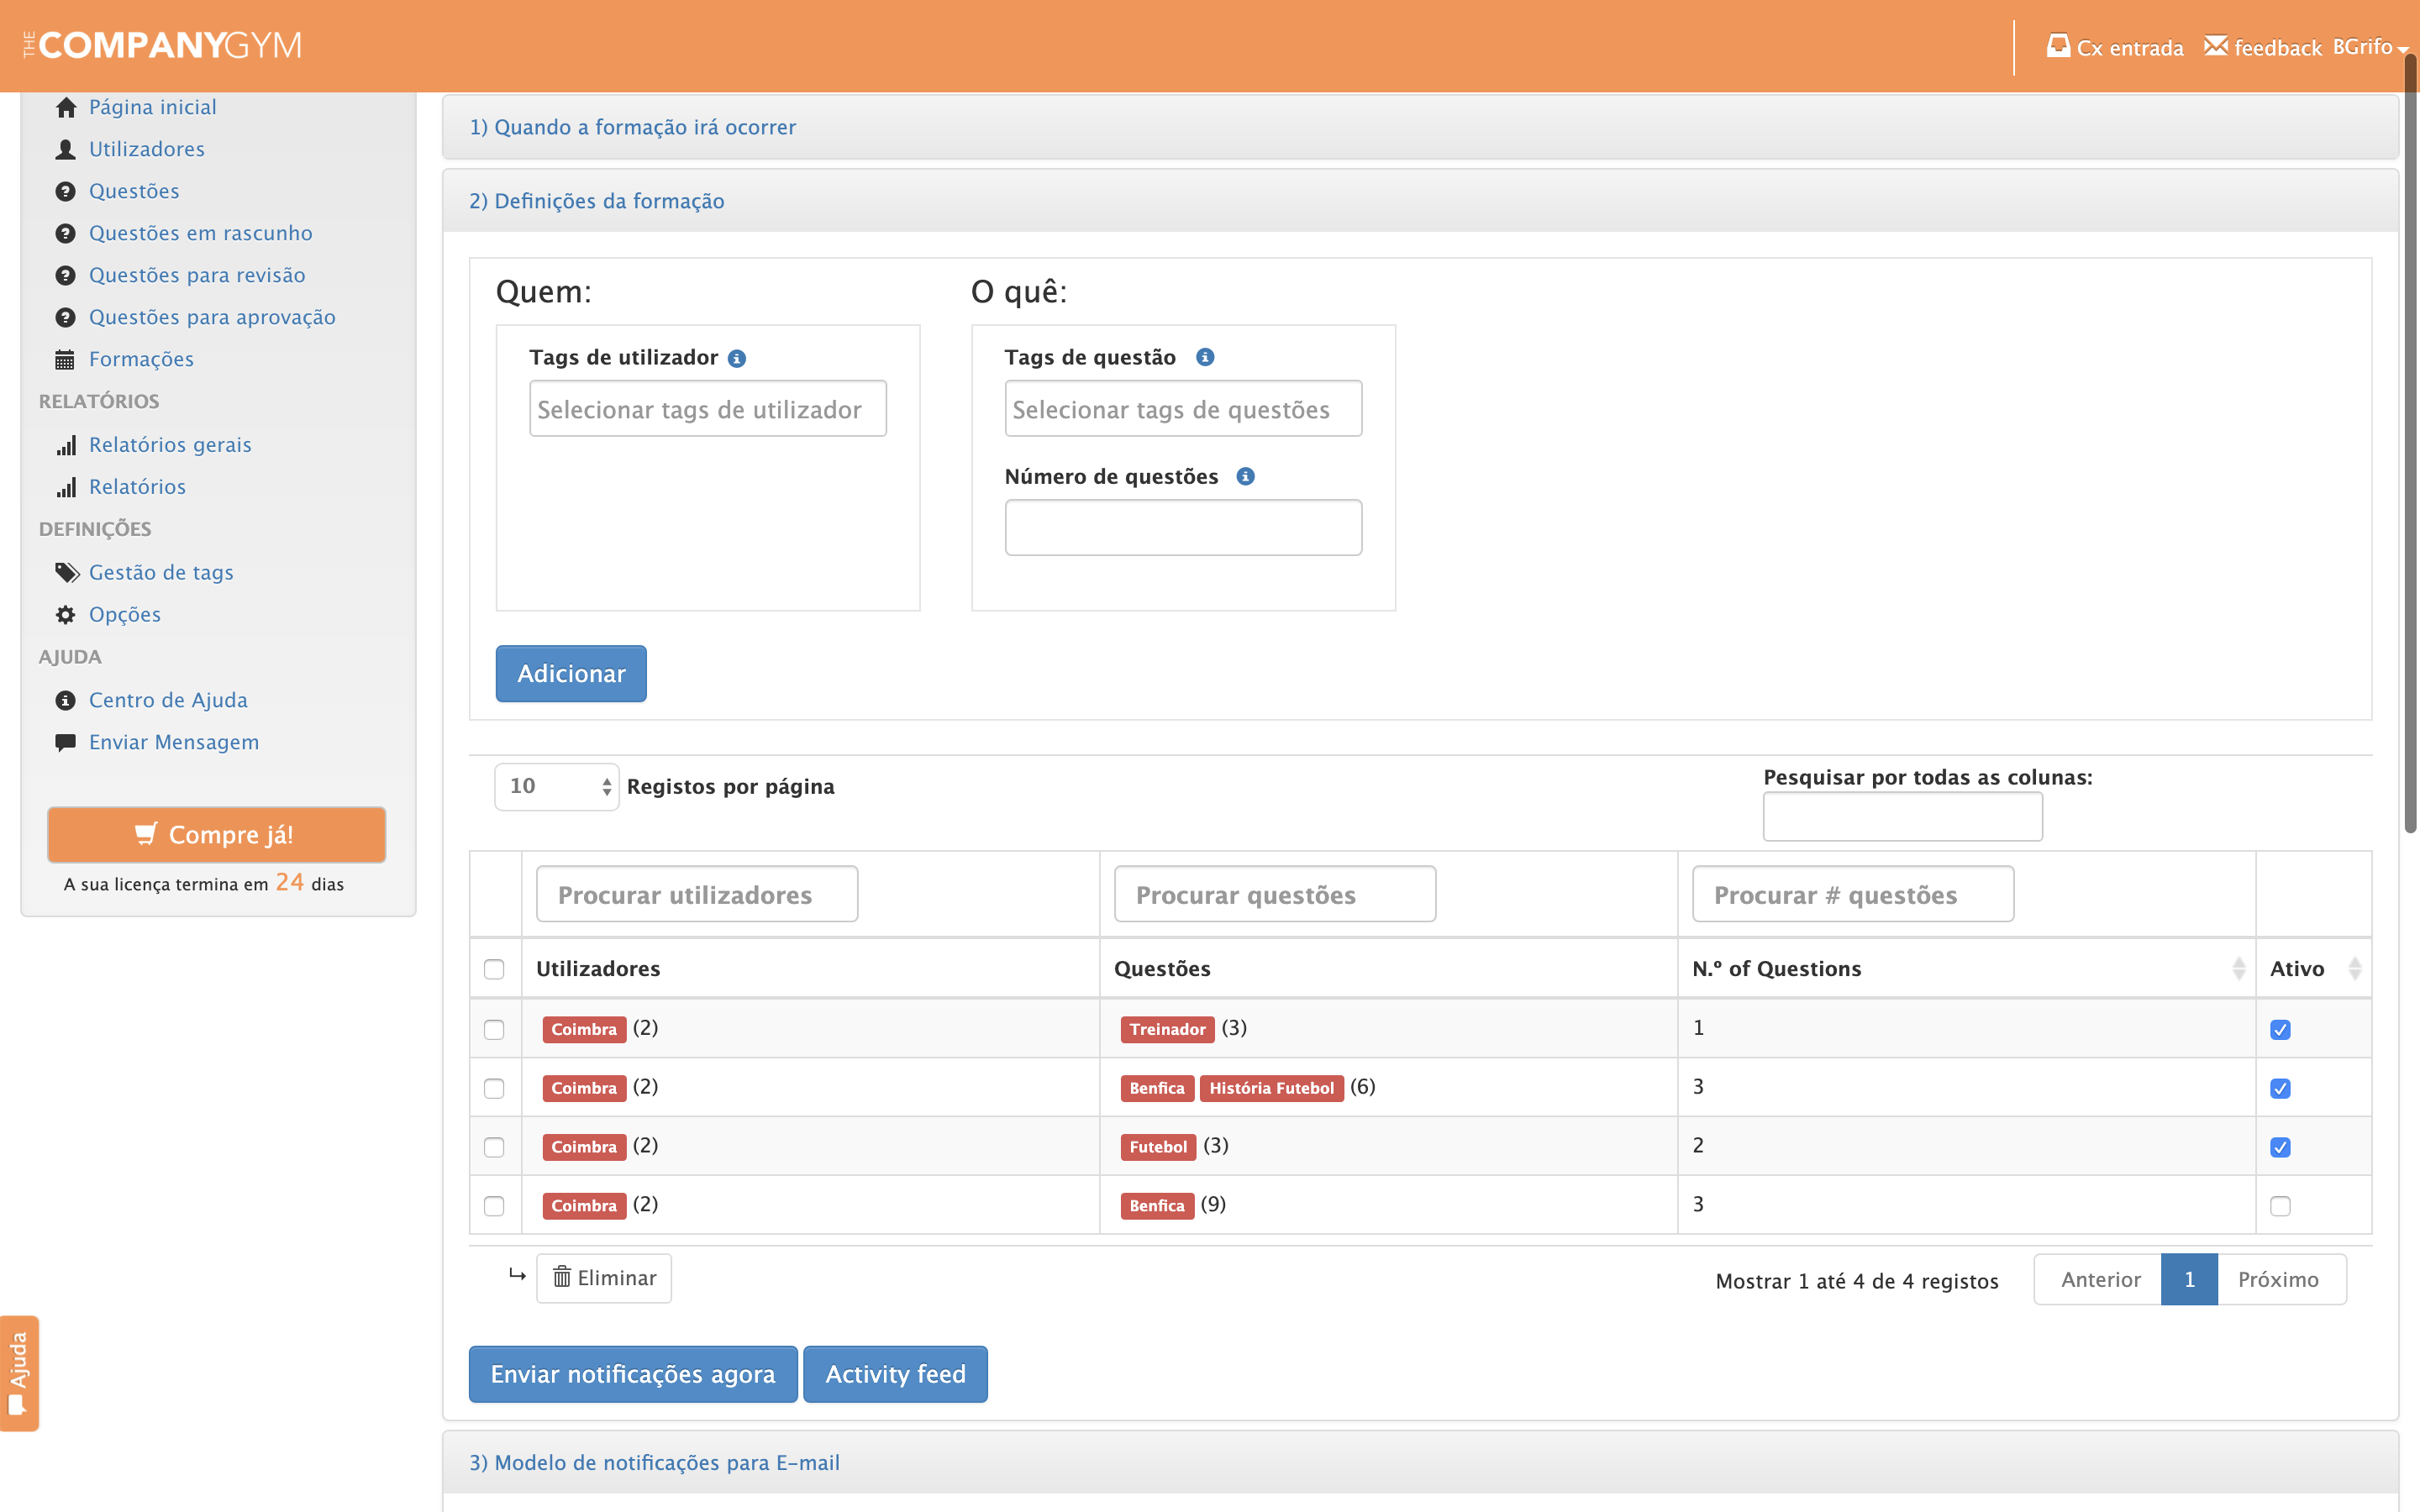
\includegraphics[width=1\textwidth]{img/tcg/tcg-form2.png}
		\caption{The Company Gym - Criar Formação (Gerir Utilizadores e Questões)}
		\label{fig:tcg-form2}
	\end{center}
\end{figure}


\newpage~\newpage


\begin{figure}[ht!]
	\begin{center}
		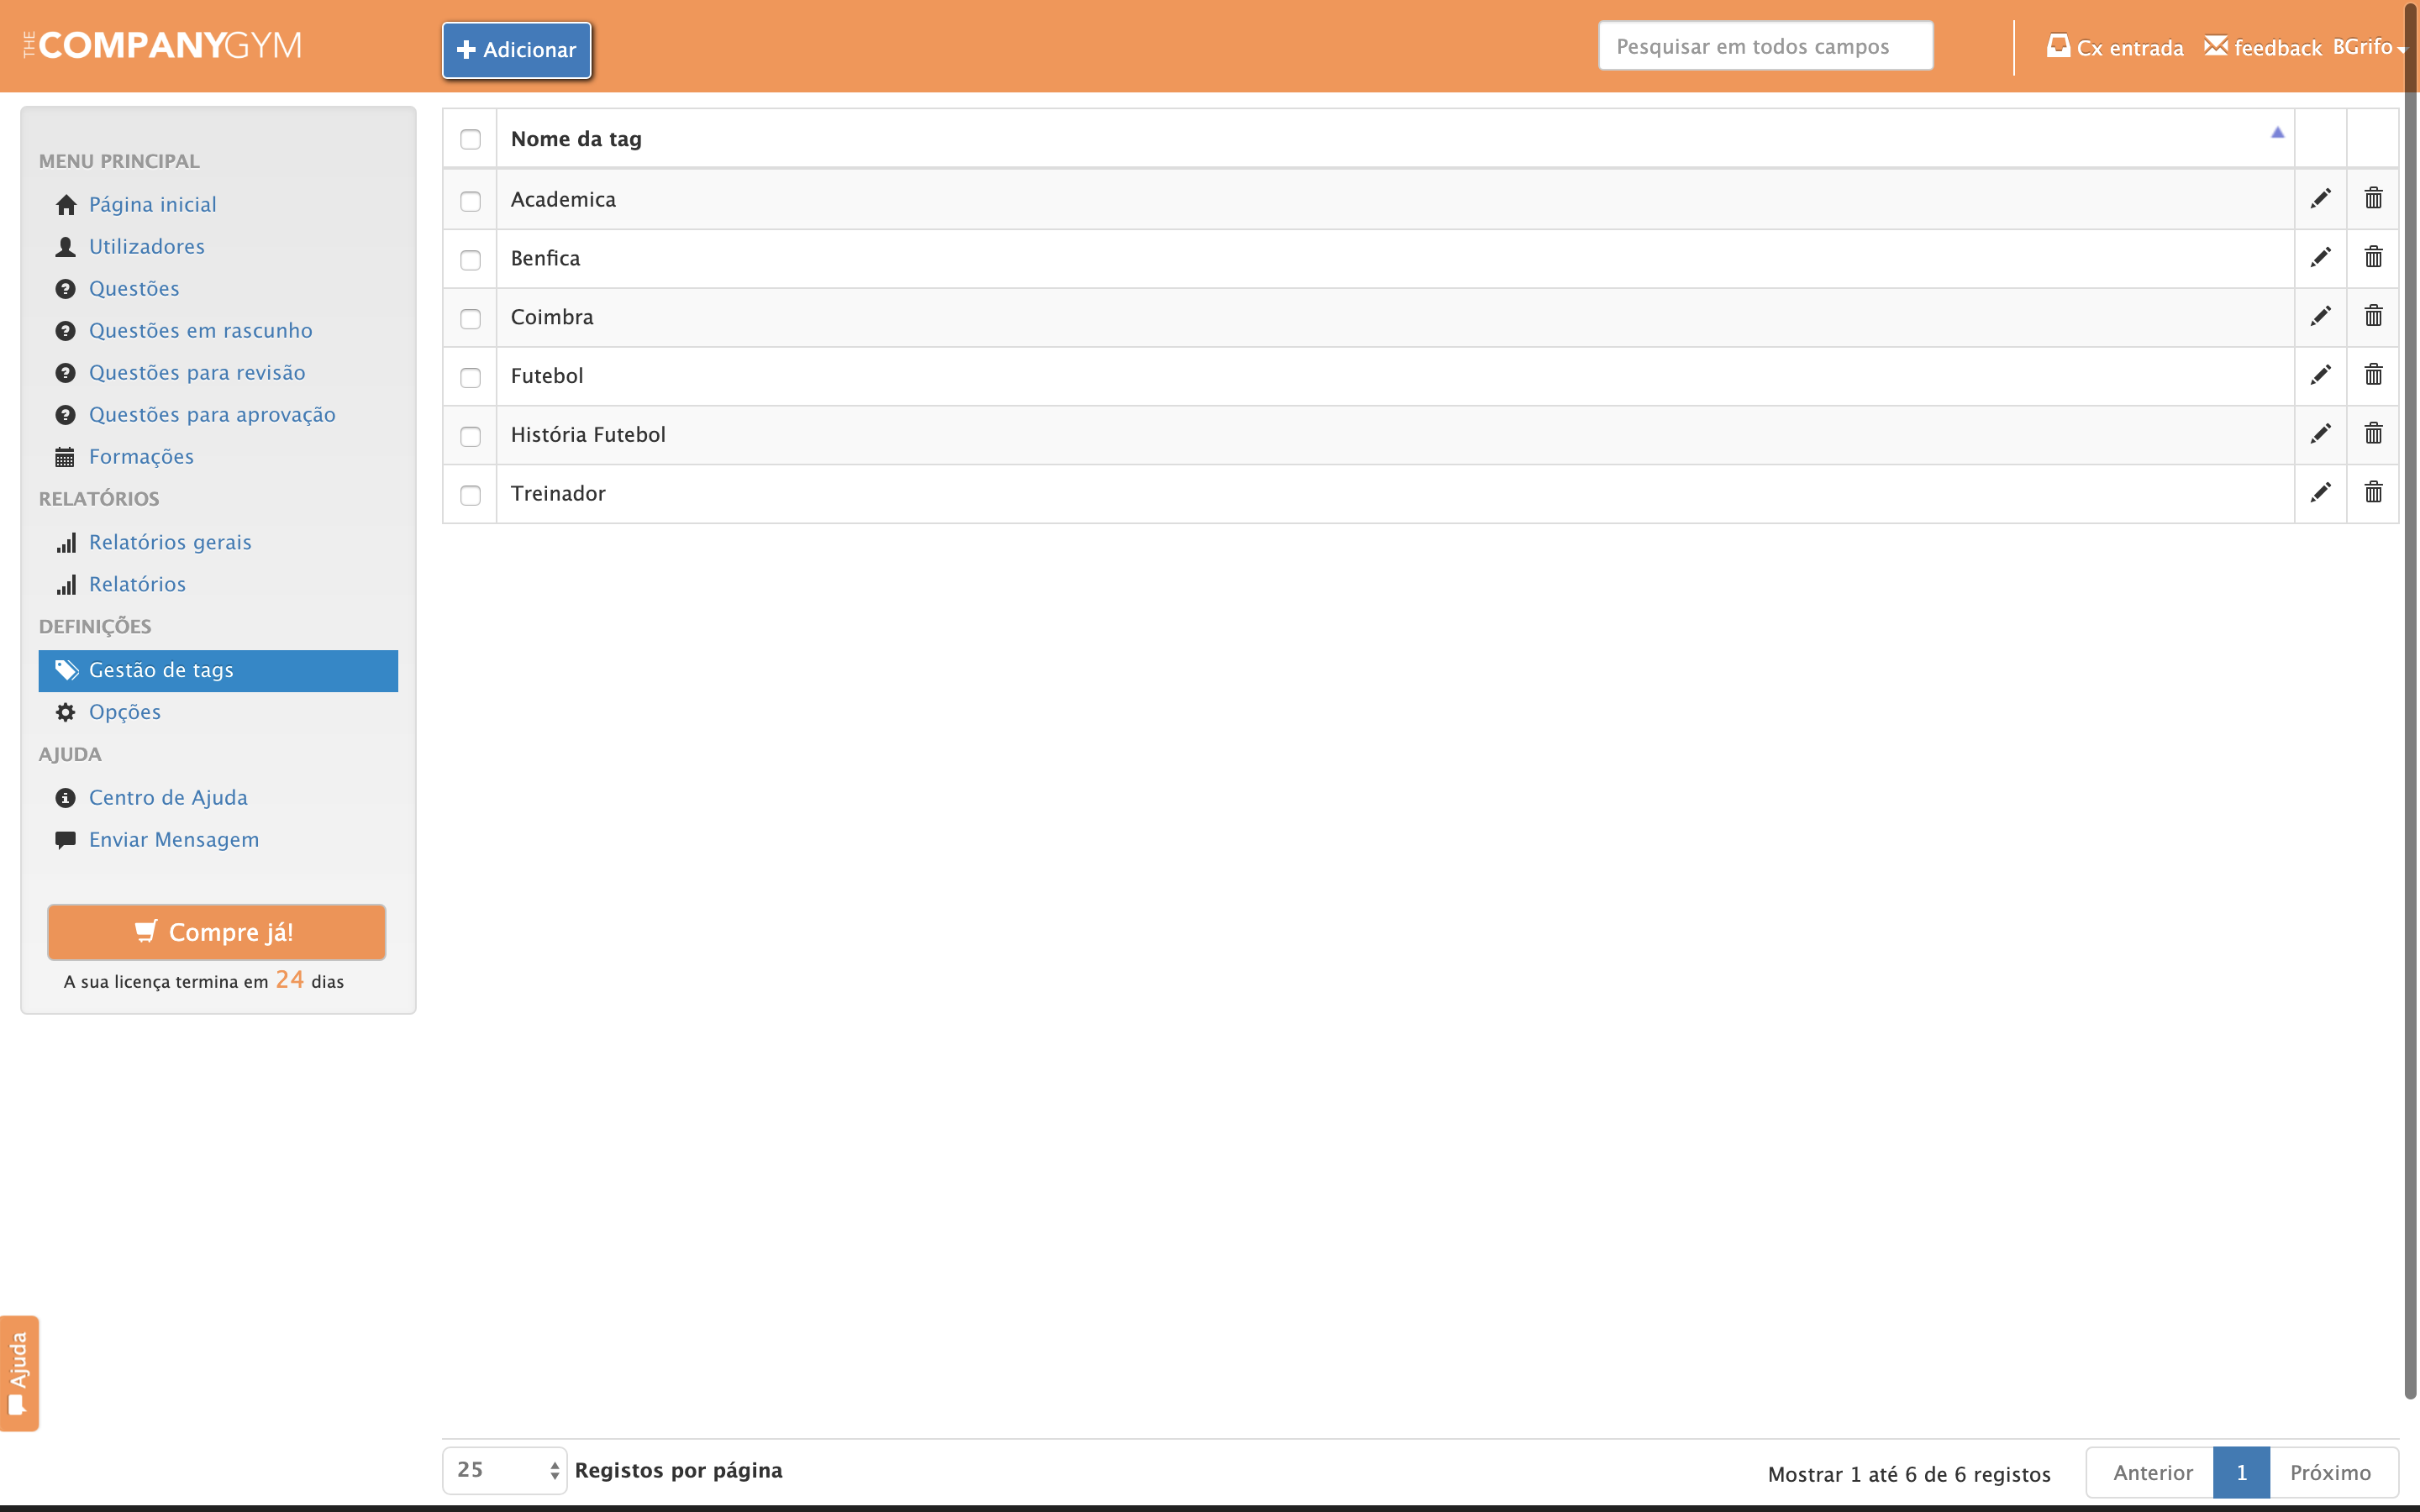
\includegraphics[width=1\textwidth]{img/tcg/tcg-tags.png}
		\caption{The Company Gym - Lista de Tags}
		\label{fig:tcg-tags}
	\end{center}
\end{figure}

É também possivel gerir todas as Tags (i. e. adicionar, editar e remover) adicionadas pelo utilizador no sistema como podemos ver na Figura \ref{fig:tcg-tags} e alterar o template do mail que é enviado para os clientes finais com o link para a formação. 

\begin{figure}[ht!]
	\begin{center}
		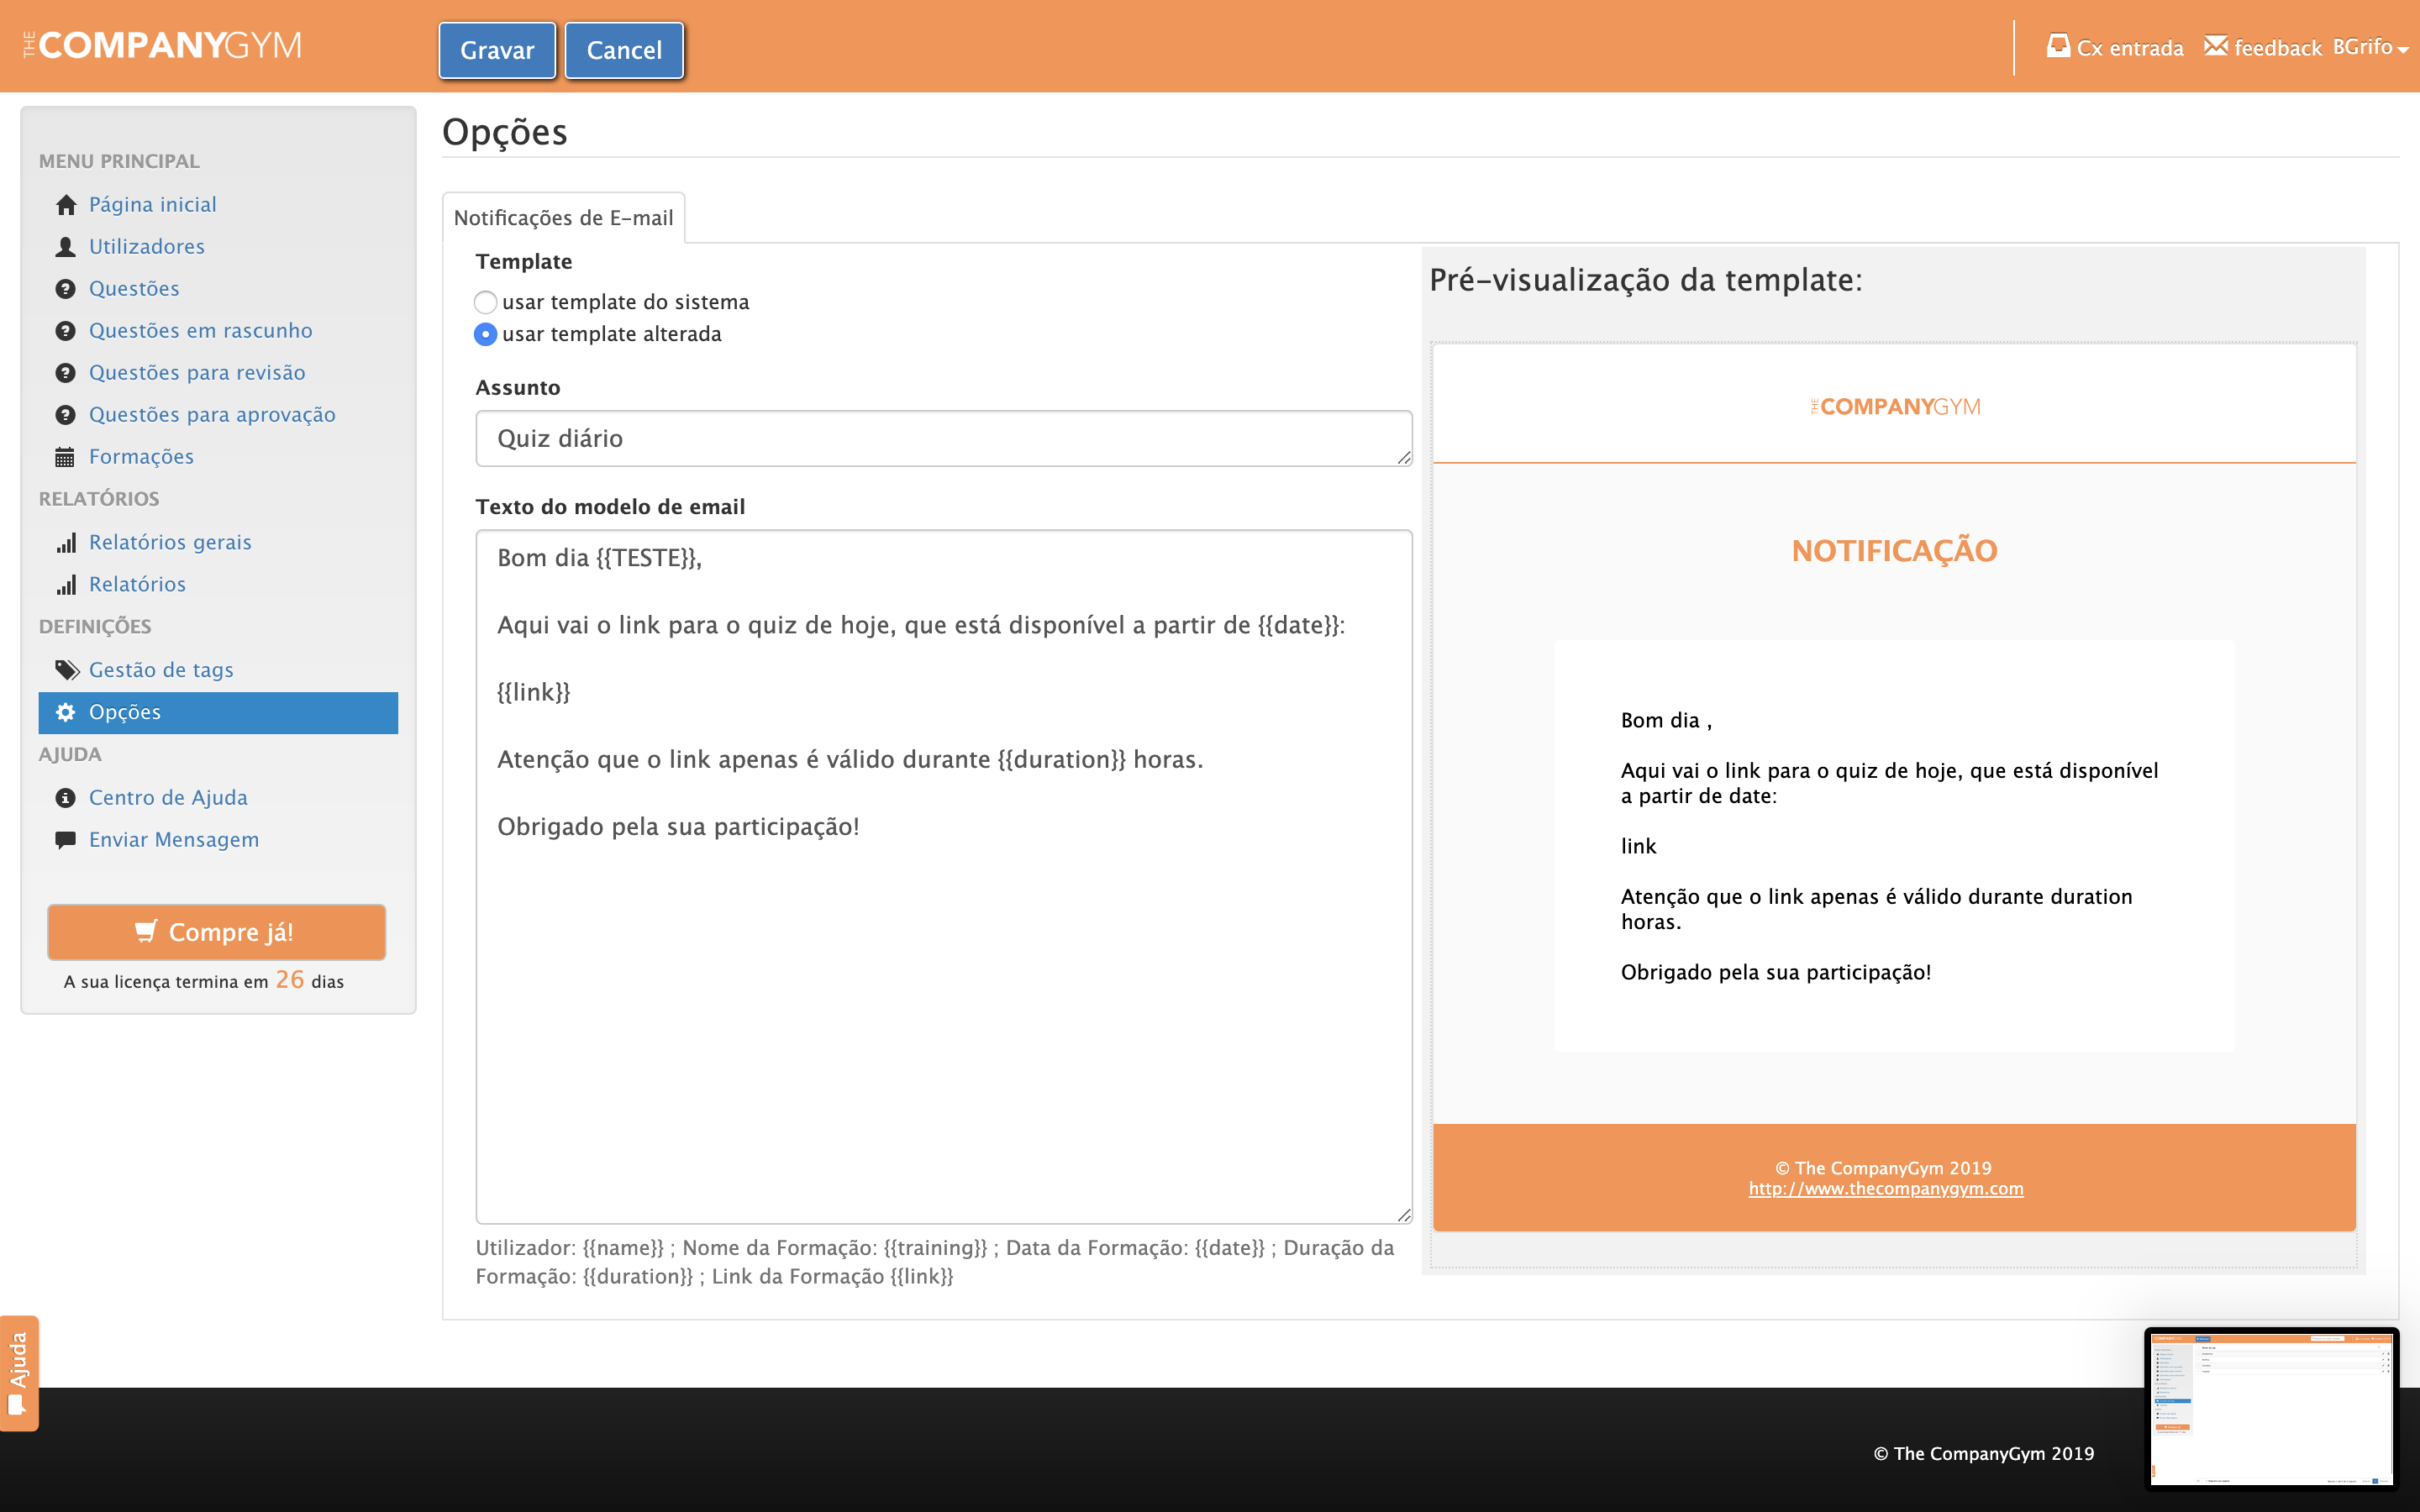
\includegraphics[width=1\textwidth]{img/tcg/tcg-mail.png}
		\caption{The Company Gym - Alterar template do mail}
		\label{fig:tcg-mail}
	\end{center}
\end{figure}

falta falar de:
relatorios
abordat messagens directas


\section{Discussão de funcionalidades}
\label{comparacao}

Nas Tabelas \ref{tab:comparacao1} e \ref{tab:comparacao} encontra-se a comparação entre as ferramentas analisadas nos secções \ref{surveyMonkey}, \ref{typeform} e \ref{googleform}, baseada numa lista de funcionalidades.

Como vimos anteriormente em todas as plataformas/ferramentas é necessário criar uma conta para aceder a todas as funcionalides e em todas as plataformas analisadas é possível criar conta e iniciar sessão através de sistemas externos (\acrshort{api}). O Projecto a desenvolver segue um modelo \acrshort{b2b} e por isso mesmo não é de grande importancia implementar esse tipo de funcionalidades pelo que, devido à sua relevância, não foi referido na Tabela \ref{tab:comparacao}.

O plataforma da Google fornece, no plano gratuito, todas as funcionalidades, ao contrário de todas as ferramentas analisadas anteriormente, que, tal como se passará com a plataforma a desenvolver, para se ter acesso a todas as funcionalidades, ou pacotes de funcionalidades, terá de ser paga uma subscrição.

Todas as platafomas permitem a criação de formulários do zero, e a plataforma da 10.digital não é excepção. Tal como foi definido na estratégia de negócio, os conteúdos que serão lançados nos formulários não serão da autoridade da 10.digital, a mesmos que estejamos incluídos em algum projecto relazionado. Dito isto facilmente se decidiu que a plataforma a desenvolver terá, tal como todas as outras ferramentas analisadas, a funcionalidade de poder adicionar conteúdo previamente feito de forma rápido (i. e. adicionar um ficheiro com todo o conteúdo estruturado). 


Tal como foi referido no capítulo \ref{sec:introducao}, secção \ref{subsec:contexto}, o inbound é uma estratégia de marketing que se foca em criar razões para os publico alvo vir até nós através da criação de conteúdo interessante, útil, relevante etc... Para manter esta procura por parte dos clientes é necessário haver valor ao longo da jornada e ideialmente proporcionar uma boa experiência ao utilizador. Nesta medida a personalização dos formulários é muito importante tanto a nível de conteúdo como estético e funcional para que o utilizador se sinta valorizado. Para tornar isto possível, tal como o SurveyMonkey e o Typoform, a plataforma a desenvolver será a algumas funcionalidades que lhe permitirá criar vários tipos de pergunta e estéticamente melhorar a experiência do utilizador final.

Antes de enviar/partilhar um formulário é sempre importante pré-visualizar e testar. Neste aspecto a platforma a desenvolver não é diferente e em relação ao envio de formulários, ao contrário de todas as outras ferramentas será possível definir uma rotina, podendo enviar formulários todos os dias, semanas ou meses, a uma hora a definir.

Por fim temos a analise e tratamento de dados que é um dos suportes daquilo que é o tripé do marketing digital. Como será de esperar a plataforma a desenvolver, tal como todas as restantes plataformas analisadas, não é um software dedicado à analise e tratamento de dados, na medida que terá limitações, contudo, ao contrário do Typeform e do Google Form, terá as funcionalidades necessárias para satisfazer as necessidades do utilizador. Analisando mais em detalhe a plataforma SurveyMonkey, que das ferramentas analisadadas, foi a única que apresentou capacidade de filtrar e segmentar os dados recolhidos, será necessário perceber que funcionalidades podemos melhorar e o que podemos acrescentar. (FALTA FALAR NA PARTILHA DE DADOS )

10.digital dá para dar feedback a cada pergunta
Falar de um exemplo de resultado dos quesitonários e dar como exemplo dois dos sites que utilizei

	\renewcommand{\arraystretch}{2.5}
\setlength\arrayrulewidth{1.5pt}
\begin{table}[!ht]  
	\begin{center}
	\begin{tabular}{|p{4cm}|p{1.5cm}|p{1.5cm}|p{1.5cm}|p{1.5cm}|}
		\cline{2-5}
		\multicolumn{1}{c|}{} & \hspace{0.6cm}\begin{sideways}SurveyMonkey.\end{sideways} & \hspace{0.6cm}\begin{sideways}Typeform\end{sideways} & \hspace{0.6cm}\begin{sideways}Google Form\end{sideways} &\hspace{0.6cm}\begin{sideways} 10.digital\end{sideways}\\ \hline
		
		
			Plano Gratuito & \cellcolor{yellow!80}   & \cellcolor{yellow!80}  & \cellcolor{green!80} & \cellcolor{yellow!80}  \\ \hline
		
		Criar Formulário do zero & \cellcolor{green!80}  & \cellcolor{green!80}  & \cellcolor{green!80} & \cellcolor{green!80} \\ \hline
		
		Templates de formulários disponíveis& \cellcolor{green!80}  & \cellcolor{green!80} & \cellcolor{green!80} & ???? \\ \hline
		
		Adicionar conteúdo previamente feitos & \cellcolor{green!80}   & \cellcolor{red!80}  & \cellcolor{green!80} & \cellcolor{green!80}  \\ \hline
		
		Tipos de perguntas & \cellcolor{green!80}  & \cellcolor{green!80}  & \cellcolor{yellow!80} & \cellcolor{green!80}  \\ \hline
		
					
	\end{tabular}
\end{center}
		\hspace{1.2cm}	\textcolor{red}{$\blacksquare$} Funcionalidade não implementada
		
	   \hspace{1.2cm}     \textcolor{yellow}{$\blacksquare$} Funcionalidade parcialmente implementada
	   
	    \hspace{1.2cm}     \textcolor{green}{$\blacksquare$} Funcionalidade totalmente implementada 
	   \begin{center}
\caption{Tabela de comparações de funcionalidades}
\label{tab:comparacao1}
\end{center}
\end{table}

\newpage
		

		\renewcommand{\arraystretch}{2.5}
		\setlength\arrayrulewidth{1.5pt}
	\begin{table}[!ht]  
		\begin{center}
		\begin{tabular}{|p{4cm}|p{1.5cm}|p{1.5cm}|p{1.5cm}|p{1.5cm}|}
			\cline{2-5}
			\multicolumn{1}{c|}{} & \hspace{0.6cm}\begin{sideways}SurveyMonkey.\end{sideways} & \hspace{0.6cm}\begin{sideways}Typeform\end{sideways} & \hspace{0.6cm}\begin{sideways}Google Form\end{sideways} &\hspace{0.6cm}\begin{sideways} 10.digital\end{sideways}\\ \hline
			
		
				\textit{Drag and Drop} & \cellcolor{green!80}   & \cellcolor{red!80}  & \cellcolor{red!80} & \cellcolor{red!80} \\ \hline
				
			% Recomendações de perguntas& \cellcolor{green!80}  & \cellcolor{green!80}  & \cellcolor{blue!25} & \cellcolor{blue!25}  \\ \hline
			Personalização do formulário& \cellcolor{green!80}    & \cellcolor{green!80}   & \cellcolor{yellow!80} & \cellcolor{green!80}   \\ \hline
			
			 Pré-visualização do formulário& \cellcolor{green!80}  & \cellcolor{green!80}  & \cellcolor{green!80} & \cellcolor{green!80} \\ \hline
			 
			 	Deixar \textit{feedback} sobre as perguntas do formulário& \cellcolor{red!80}    & \cellcolor{red!80}   & \cellcolor{red!80} & \cellcolor{green!80}   \\ \hline
			
			 Integração de sistemas externos& \cellcolor{red!80}   & \cellcolor{green!80} & \cellcolor{yellow!80}  & ????  \\ \hline
			
			Envio do formulário de forma periódica & \cellcolor{red!80}   & \cellcolor{red!80}  & \cellcolor{red!80} & \cellcolor{green!80} \\ \hline
			
			 Analise de resultados & \cellcolor{green!80}   & \cellcolor{yellow!80} & \cellcolor{yellow!80} & \cellcolor{green!80}  \\ \hline
			
			Partilha dos resultados & \cellcolor{green!80}   & \cellcolor{green!80}   & \cellcolor{green!80}  & ???? \\ \hline
			
			Exportar os resultados & \cellcolor{green!80}   & \cellcolor{green!80}   & \cellcolor{green!80}  & \cellcolor{green!80}  \\ \hline
			
			
		\end{tabular}
	\end{center}
\hspace{1.2cm}	\textcolor{red}{$\blacksquare$} Funcionalidade não implementada

\hspace{1.2cm}     \textcolor{yellow}{$\blacksquare$} Funcionalidade parcialmente implementada

\hspace{1.2cm}     \textcolor{green}{$\blacksquare$} Funcionalidade totalmente implementada 
\begin{center}
	\caption{Tabela de comparações de funcionalidades}
	\label{tab:comparacao}
\end{center}
	\end{table}


%-------------------------------------------------------------------------------------------------
\blankpage
%-------------------------------------------------------------------------------------------------

\glsresetall




\chapter{Abordagem}
\label{sec:abordagem}

Este capítulo tem como principal objectivo descrever a metodologia adotada e ainda apresentar o planeamento do projeto tal como os desvios relativamente ao mesmo. Por fim será apresentada uma análise dos riscos associados ao projeto que poderão ter um impacto negativo no plano de desenvolvimento. Este conjunto de passos foca-se em atingir um produto final bem estruturado e funcional, utilizando boas práticas de desenvolvimento de software


\section{Metodologia}
\label{metodologia}

A metodologia de desenvolvimento do projeto adoptada foi uma metodologia fortemente baseada em SCRUM\cite{scrum}, que será descrita (i. e. os aspectos mais importantes) nesta secção. Esta é a metodologia utilizada pela 10.digital e tendo em conta que esta metodologia ágil se encaixa perfeitamente nas necessidades do projeto, estes foram os fatores decisivos para a escolha da mesma. 

Líder em desenvolvimento ágil, o SCRUM, é uma metodologia apontada para projetos com foco em trazer valor ao cliente de forma incremental, através de iterações de curta duração, chamadas \textit{Sprints}. Esta metodologia possibilita também a abordagem de problemas complexos de forma produtiva, priorizar tarefas durante a fase de desenvolvimento e ainda facilita a inclusão de novas funcionalidades sempre que necessário. Desta forma o SCRUM proporciona uma gestão flexível do projeto e permite realizar pequenas alterações no planeamento, sem necessidade de interromper o desenvolvimento.

\subsection{Intervenientes}

Um aspecto determinante para o sucesso do SCRUM é o trabalho em equipa. Tipicamente nesta metodologia existem três papéis pré-definidos: \textit{Product Owner}, \textit{Scrum Master} e \textit{Scrum Team}.

O \textbf{\textit{Product Owner}} representa o cliente e é responsável por transmitir a visão do produto, ou por outras palavras, é responsável por maximizar o valor do produto e o trabalho da equipa de desenvolvimento (i. e. \textit{Scrum Master}). É responsável por organizar e priorizar as tarefas no \textit{product backlog}.

O \textbf{\textit{Scrum Master}} tem um papel fundamental no desempenho da \textit{Scrum Team}. É responsável por garantir o cumprimento das práticas do SCRUM, ajudar e orientar a \textit{Scrum Team} especialmente nas dificuldades que vão surgindo ao longo do projeto e, de forma gradual (i. e. respeitando as \textit{Sprints}), apresentar o trabalho realizado ao \textit{Product Owner}.

A \textbf{\textit{Scrum Team}} representa os elementos que constituem a equipa de desenvolvimento que com a orientação do \textit{Scrum Master}, monitorizam o trabalho que vai sendo feito e assim conseguir cumprir com as \textit{sprints backlog}. A \textit{Scrum Team} deve ser autónoma e organizada. 

\subsection{Processo}

O Desenvolvimento começa assim que o \textit{product backlog} estiver concluído e detalhado pelo \textit{Product Owner}. O \textit{product backlog} representa a lista requisitos necessários para atingir o produto final. 

Depois de definido o \textit{product backlog}, o \textit{Scrum Master}, juntamente com a \textit{Scrum Team} reúnem e definem o tempo para cada \textit{Sprint}. Tipicamente as \textit{Sprints} tem duração entre 1 a 4 semanas e no final das mesmas é apresentado o trabalho realizado pela \textit{Scrum Team}. No início de cada \textit{Sprint} é criada a \textit{Sprint Backlog}. Na \textit{Sprint Backlog} é estipulado o conjunto de funcionalidades/tarefas a realizar durante a \textit{Sprint}. Na 10.digital a variável da velocidade não é implementada na \textit{Sprint Backlog}.

No início de cada dia é realizada a \textit{Daily Scrum}, uma reunião que tem uma duração de 15$\pm$5 minutos, onde, de forma informal, são discutidas as tarefas que devem ser implementadas nesse dia, o ponto de situação do projeto relativo ao dia anterior e caso haja algum impasse ou dificuldade na realização de alguma tarefa, imediatamente após a reunião (i. e. assim que possível) tentasse arranjar uma solução para o mesmo. 

No final de cada \textit{Sprint} há uma reunião (\textit{Sprint Review}) para verificar as tarefas que foram realizadas. Durante a reunião a \textit{Scrum Team} apresenta as novas funcionalidades implementadas para os restantes participantes que podem ser \textit{Product Owner}, \textit{Scrum Master}, clientes e outros colegas de trabalho. 

A Figura \ref{fig:scrum} sumariza todo o processo descrito anteriormente.



\begin{figure}[ht!]
	\begin{center}
		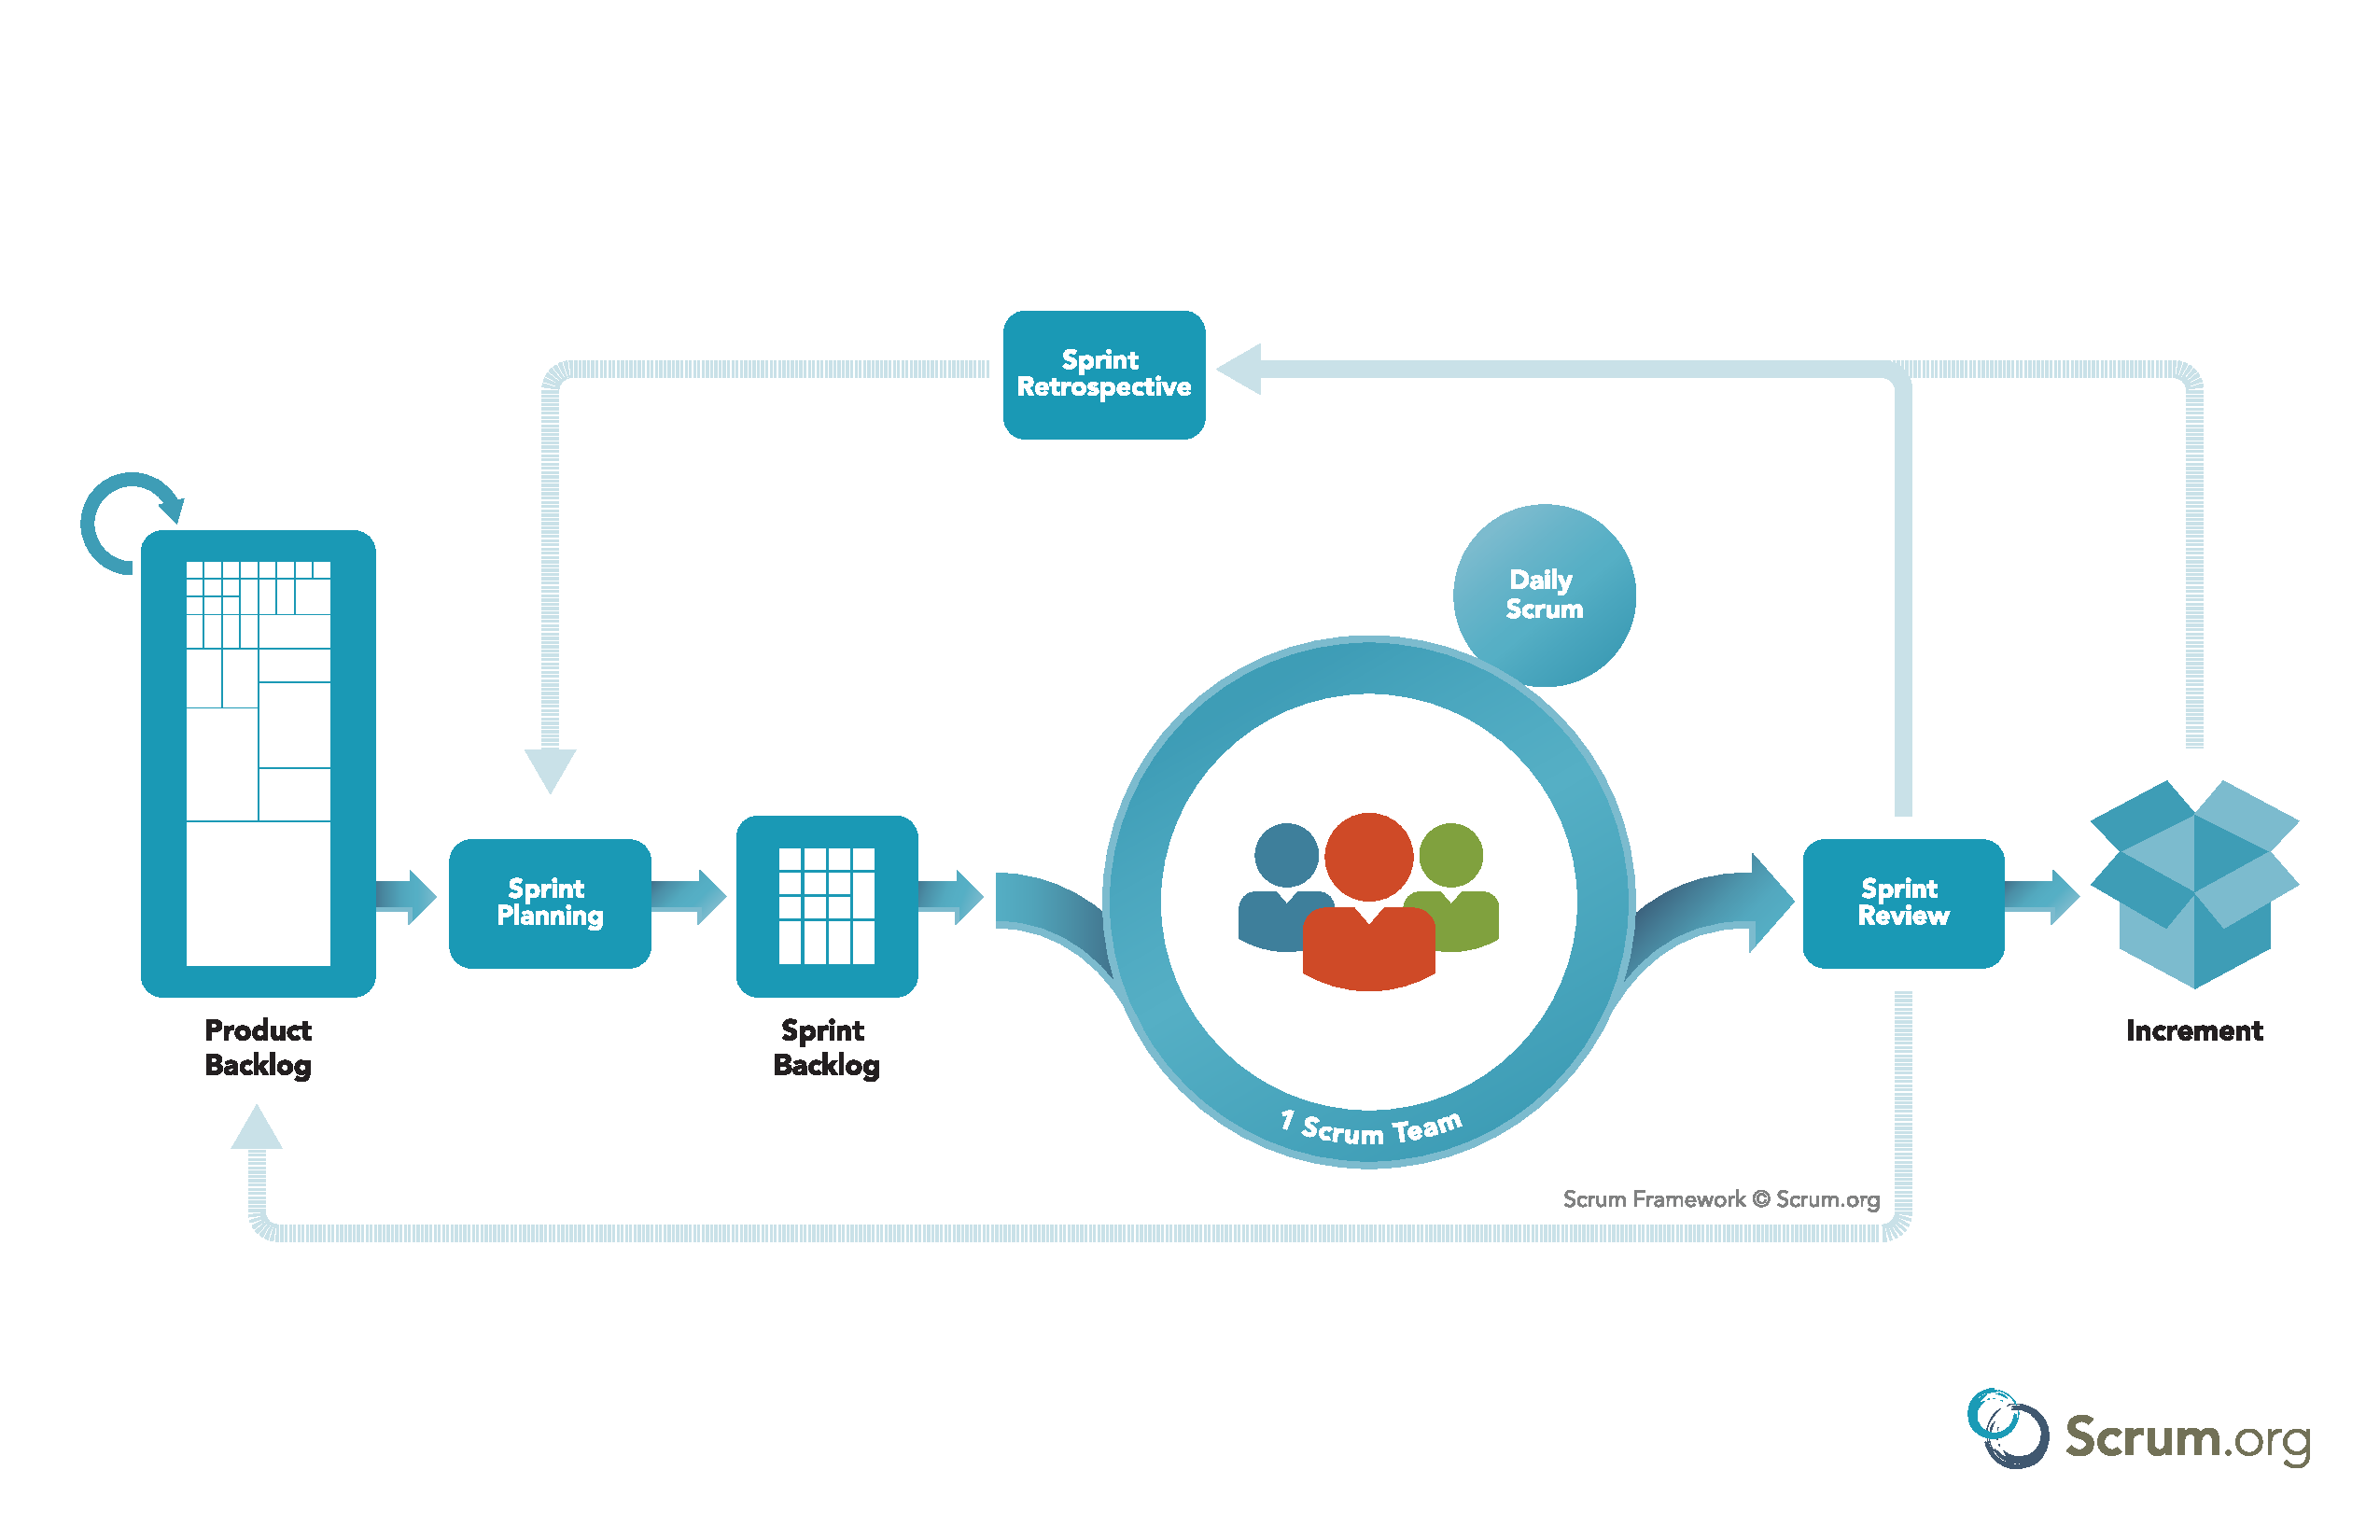
\includegraphics[width=1\textwidth]{img/scrum.pdf}
		\caption{Scrum Framework\cite{scrumimg}}
		\label{fig:scrum}
	\end{center}
\end{figure}

\newpage

\section{Planeamento}
\label{planeamento}

Nesta secção será apresentado o plano de estágio do primeiro e segundo semestre, através de diagramas de Gantt.  De seguida será exposto o desvio temporal em relação ao planeado e por fim serão brevemente detalhados os artefactos (i. e. \textit{Sprint Backlog}) da metodologia SCRUM.

Como foi referido no Capítulo \ref{sec:introducao}, este documento expõe o trabalho realizado neste projeto durante o ano lectivo, por isso, apenas será exposto o desenvolvimento do \textit{back-end} da plataforma de inbound marketing. Dito isto, a equipa de desenvolvimento será composta por múltiplas pessoas sendo que cada um terá a sua função distinta.
No seguimento do ponto anterior, os cargos de cada interveniente no projeto são:
\begin{itemize}
	\item[--] \textbf{\textit{Product Owner}}: Eng. Pedro Beck (\acrfull{cto})
	\item[--] \textbf{\textit{Scrum Master}}: Mário Melo (Coordenador de Projetos)
	\item[--] \textbf{\textit{Scrum Team}}: 
	\subitem  \textit{Front-End Developer} - Por Definir
	\subitem  \textit{Back-End Developer} - Bruno Grifo
	\subitem  \textit{Back-End Developer \acrshort{tcg}} - Eng. Pedro Beck
\end{itemize}

É ainda de referir que, no primeiro semestre, o Mestre João Oliveira realizou o papel de co-orientador na empresa e teve um impacto importante na orientação do projeto de tese. 

\begin{figure}[ht!]
	\begin{center}
		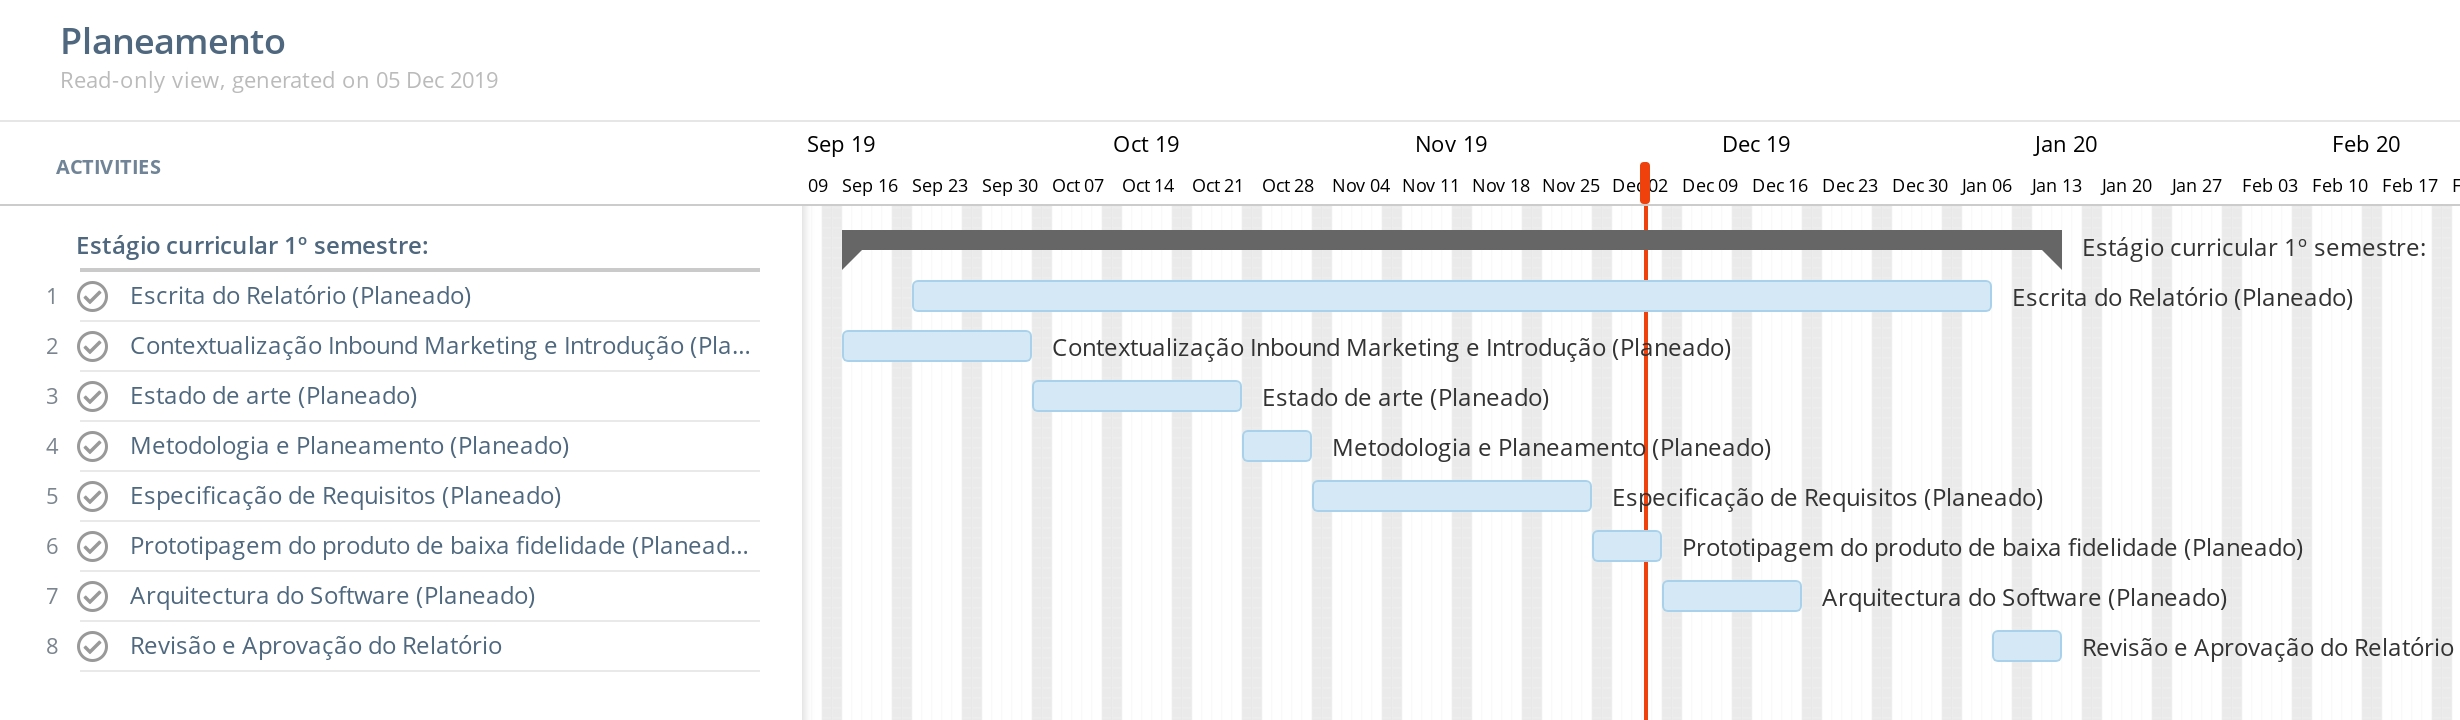
\includegraphics[width=1\textwidth]{img/gantt/semestre1.jpeg}
		\caption{Diagrama de Gantt - Planeamento do 1º semestre}
		\label{fig:gantt1}
	\end{center}
\end{figure}

Representado na Figura \ref{fig:gantt1} temos o plano de estágio relativo ao primeiro semestre. A escrita do relatório intermédio foi dividido nas seguintes 6 tarefas principais:
\begin{itemize}
	\item \textbf{Contextualização Inbound Marketing e Introdução}: Tendo em conta a àrea onde o projeto se ínsere, foi realizado um estudo sobre inbound marketing para que me pudesse contextualizar e conseguir compreender as diversas estratégias de inbound. No final da tarefa foi realizada uma apresentação sobre este tema e avaliada pelo co-orientador da empresa, para garantir o nível de conhecimento pretendido. Este estudo foi crucial para desenhar o modelo de negócio do projeto.
	\item \textbf{Estado de Arte}: Nesta tarefa foi feito o levantamento do estado de arte. Foram analisadas várias aplicações/plataformas concorrentes ou com funcionalidades semelhantes para ganhar um melhor conhecimento sobre o mercado.
	\item \textbf{Metodologia e Planeamento}: Foi feito um estudo interno para perceber ao detalhe como foi adoptada a metodologia SCRUM na empresa.
	\item \textbf{Especificação de Requisitos}: Esta tarefa começou com a elaboração de alguns protótipos de baixa fidelidade e um conjunto de requisitos funcionais. De seguida foi marcada uma reunião com o cliente onde, pegando no trabalho realizado anteriormente, foram feitos os devidos ajustes e levantado os restantes requisitos. Foram assim documentados os requisitos não funcionais, funcionais e respetivos casos de uso e ainda as restrições técnicas e de negócios.
	\item \textbf{Prototipagem de produto de baixa fidelidade}: Foi criado um conjunto de protótipos que representam todas as funcionalidades principais da plataforma e que de igual forma satisfazem o caso de uso correspondente.
	\item \textbf{Arquitectura de Software}: Nesta tarefa foi projetada a arquitectura a desenvolver no âmbito do estágio.
\end{itemize}

Neste projeto cada \textit{sprint} dura duas semanas e a \textit{sprint meeting} é feita no último dia. Em cada\textit{ sprint meeting }está presente a equipa de desenvolvimento (\textit{scrum team}), os orientadores (\textit{product owner}) e, sempre que possível, o tutor. Cada estagiário apresenta o que fez durante o \textit{sprint}, executa a \textit{demo} das funcionalidades implementadas e partilha as dificuldades encontradas durante o \textit{sprint }com os restantes. Os orientadores dão \textit{feedback}, tanto do resultado geral do \textit{sprint}, como de cada funcionalidade (\textit{user story}) implementada.


Neste semestre cada \textit{Sprint} tem a duração de 2 semanas e no final da mesma é feita uma reunião de ponto (i. e. \textit{Daily Scrum}), onde estão presentes o \textit{Product Owner}, \textit{Scrum Master}, clientes e outros colegas de trabalho que queiram participar. Nesta primeira fase, no total foram realizadas 7 \textit{Sprints}:

\begin{itemize}
	\item \textbf{\textit{Sprint} \#1}
		\subitem \textbf{Data Início}: 16/09/2019
		\subitem \textbf{Data Fim}: 27/09/2019
		\subitem \textbf{Descrição}: Estudo sobre Inbound Marketing.
	\item \textbf{\textit{Sprint} \#2}
		\subitem \textbf{Data Início}: 28/09/2019
		\subitem \textbf{Data Fim}: 11/10/2019
		\subitem \textbf{Descrição}: Escrita do Capítulo \ref{sec:introducao} e início do estudo sobre aplicações/plataformas concorrentes.
	\item \textbf{\textit{Sprint} \#3}
		\subitem \textbf{Data Início}: 12/10/2019
		\subitem \textbf{Data Fim}: 25/10/2019
		\subitem \textbf{Descrição}: Conclusão do estudo de mercado e escrita do Capítulo \ref{sec:estado-arte}.
	\item \textbf{\textit{Sprint} \#4}
		\subitem \textbf{Data Início}: 26/10/2019
		\subitem \textbf{Data Fim}: 08/11/2019
		\subitem \textbf{Descrição}: Escrita do Capítulo \ref{sec:abordagem} e reunião com o cliente para levantamento de requisitos.
	\item \textbf{\textit{Sprint} \#5}
		\subitem \textbf{Data Início}: 09/11/2019
		\subitem \textbf{Data Fim}: 22/11/2019
		\subitem \textbf{Descrição}: Escrita do Capítulo \ref{sec:requisitos}.
	\item \textbf{\textit{Sprint} \#6}
		\subitem \textbf{Data Início}: 23/11/2019
		\subitem \textbf{Data Fim}: 06/12/2019
		\subitem \textbf{Descrição}:  Escrita dos casos de Uso no Anexo \ref{a:cu} e prototipagem do produto de baixa fidelidade no Anexo \ref{a:prototipos}.
	\item \textbf{\textit{Sprint} \#7}
		\subitem \textbf{Data Início}: 06/11/2019
		\subitem \textbf{Data Fim}: 20/12/2019
		\subitem \textbf{Descrição}: Projeção da arquitectura e escrita do Capítulo \ref{sec:arquitetura}
\end{itemize}

\begin{figure}[ht!]
	\begin{center}
		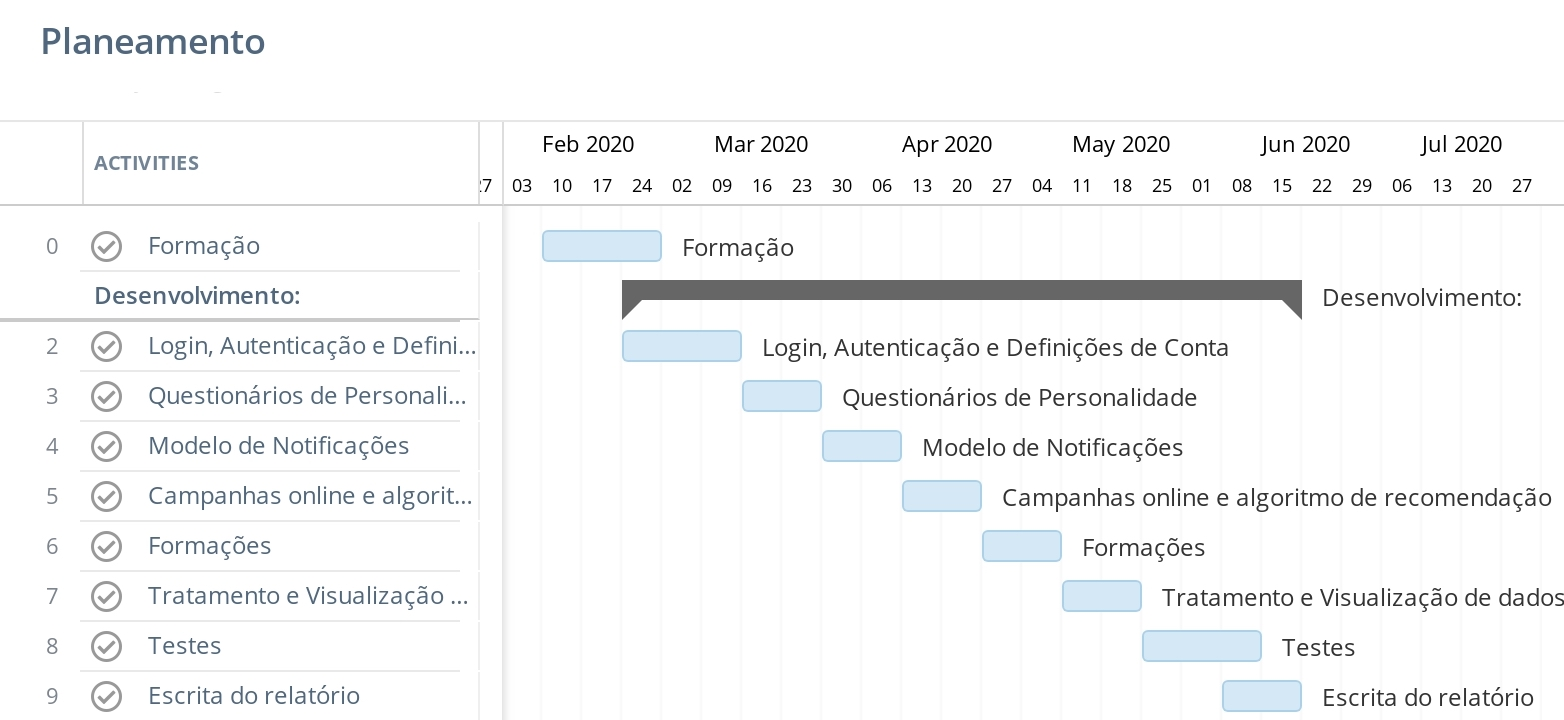
\includegraphics[width=1\textwidth]{img/gantt/semestre2.jpeg}
		\caption{Diagrama de Gantt - Planeamento do 2º semestre}
		\label{fig:gantt2}
	\end{center}
\end{figure}

Representado na Figura \ref{fig:gantt2} temos o plano de estágio relativo ao segundo semestre. A fase de implementação divide-se em várias \textit{Sprints}, que serão detalhadas no Capítulo \ref{sec:sprints}.

\newpage

\begin{figure}[ht!]
	\begin{center}
		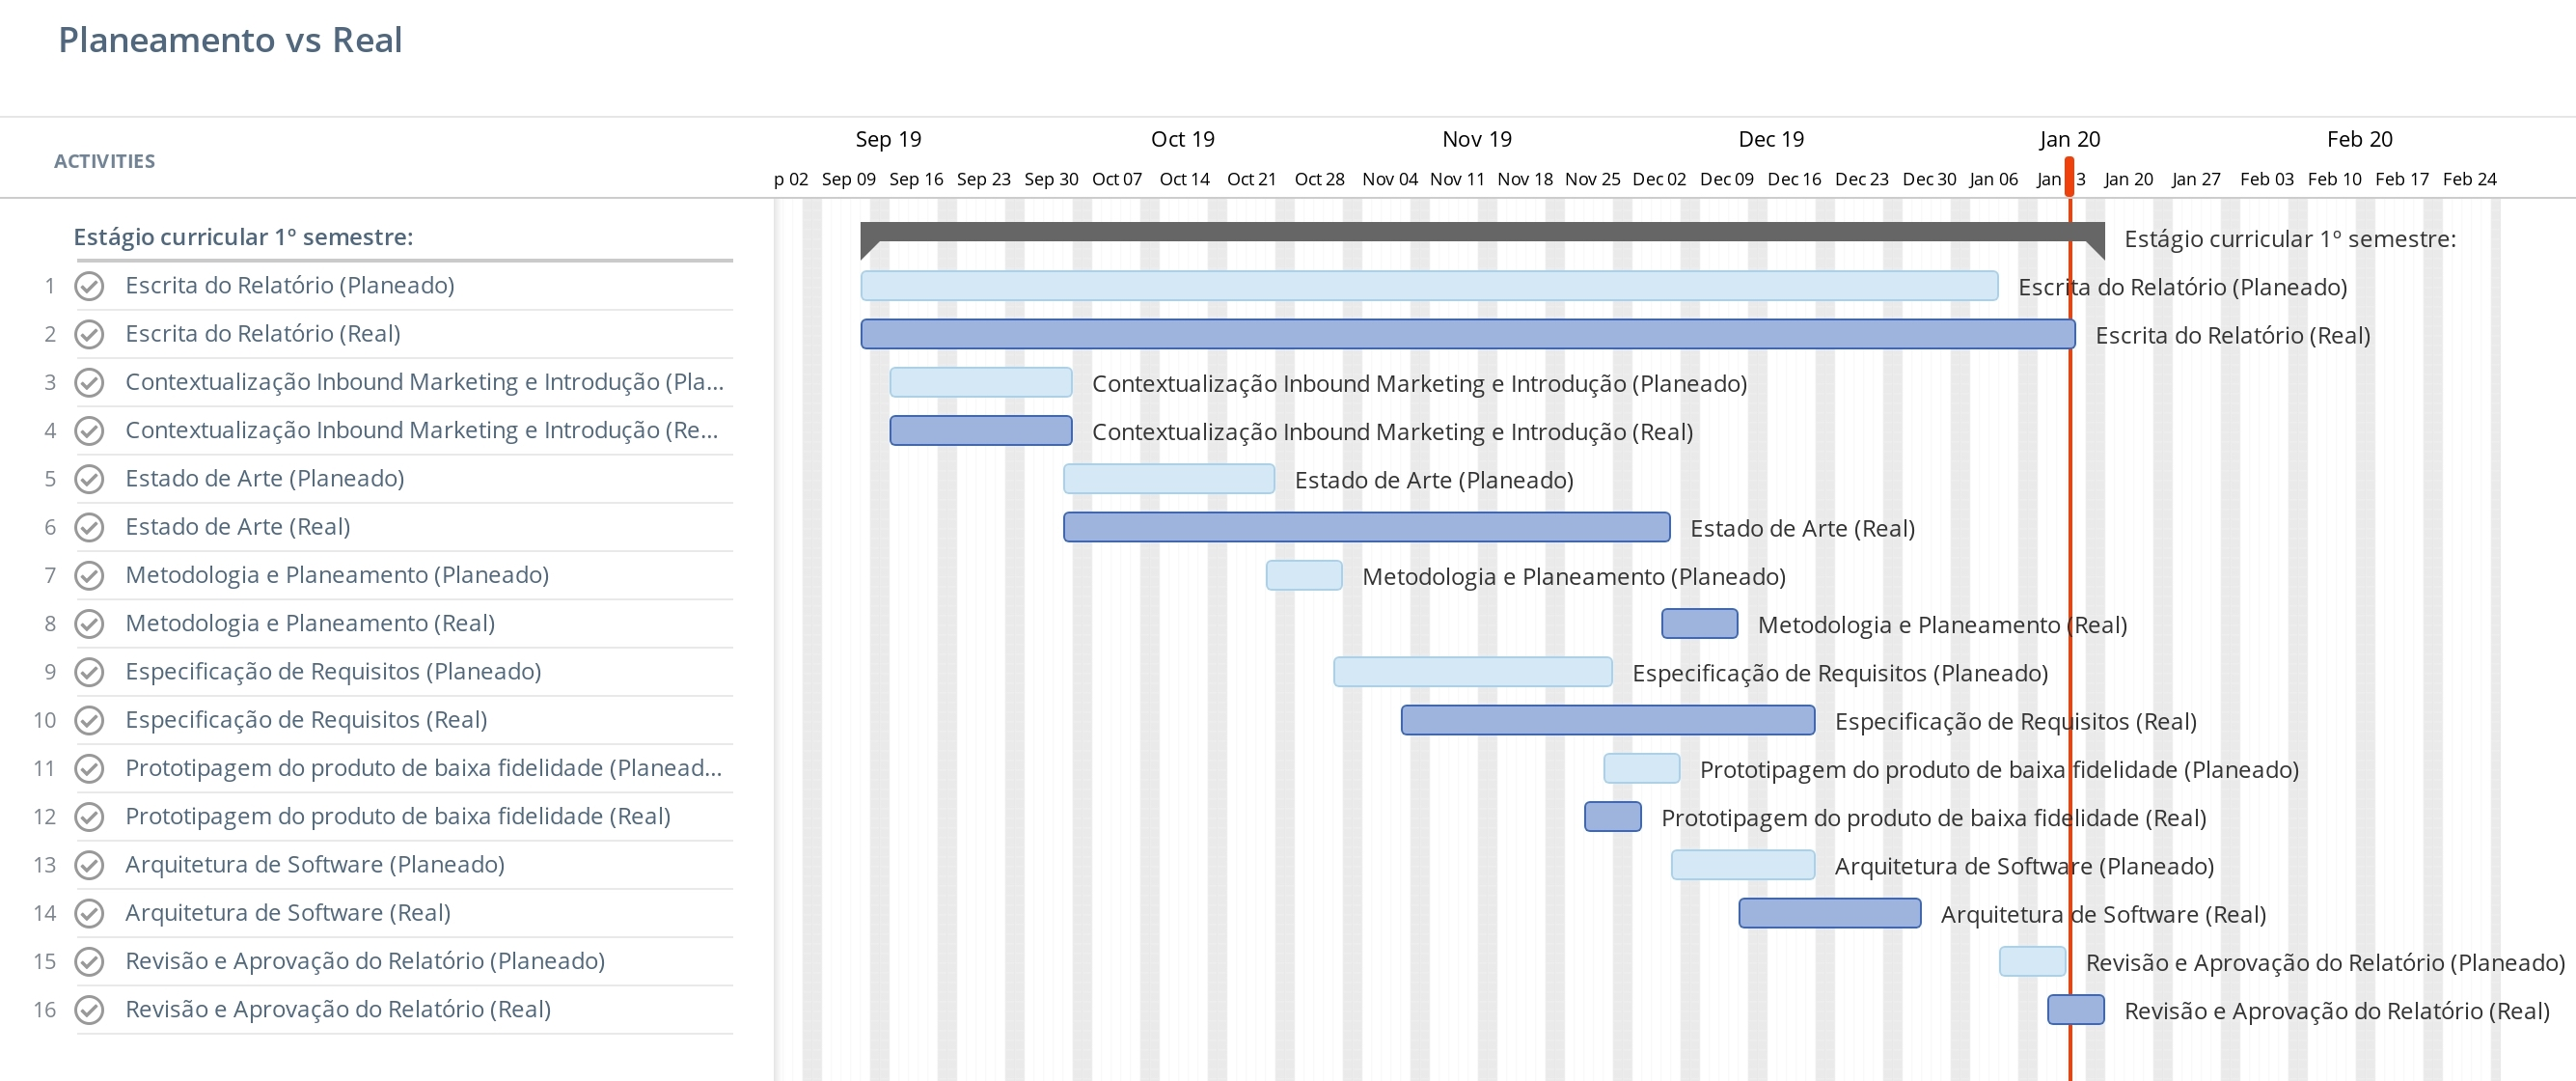
\includegraphics[width=1\textwidth]{img/gantt/vs.jpeg}
		\caption{Diagrama de Gantt - Planeamento vs Real do 1º semestre}
		\label{fig:ganttvs1}
	\end{center}
\end{figure}

Representado na Figura \ref{fig:ganttvs1} temos o planeamento de estágio relativo ao primeiro semestre em comparação com o tempo que o aluno realmente demorou a concluir as tarefas. A primeira tarefa que salta à vista é o Estado de Arte, que claramente excedeu a data limite de entrega para a reunião de ponto com os orientadores de estágio. Um dos fatores decisivos para o atraso na realização da tarefa deveu-se ao facto de ser uma fase de pesquisa e análise do mercado atual, em que é difícil de prever o tempo exato que se demora a realizar esta tarefa. O outro fator decisivo deveu-se ao facto de, a meio do semestre, o cliente ter pedido para implementar uma nova funcionalidade que representa um dos principais objetivos na plataforma a desenvolver. Tudo isto criou um atraso significativo em todas as restantes tarefas. Podemos também reparar que a escrita da tarefa da Metodologia e Planeamento foi realizada algumas semanas depois do planeado. O aparecimento da nova funcionalidade levou a uma reestruturação do planeamento o que provocou um atraso nesta tarefa, visto que só se inicializou a escrita da mesma depois de ter acabar o novo planeamento.



\glsresetall




\chapter{Especificação de Requisitos}
\label{sec:requisitos}

O processo de especificação de requisitos é crucial para o desenvolvimento de um projeto de \textit{software}, devendo dar atenção tanto aos requisitos funcionais como aos requisitos não funcionais.

Este capítulo apresenta os requisitos que foram identificados e analisados para a plataforma e define um conjunto de diretrizes que devem ser seguidas durante o desenvolvimento do projeto. Estes requisitos foram definidos e identificados com base em reuniões com o cliente e na análise de soluções, actualmente no mercado, que partilham funcionalidades semelhantes com a plataforma que vai ser desenvolvida

Este capítulo divide-se em 3 secções. A secção \ref{requisitos:tiposutilizadores} identifica as principais partes envolventes no projeto (i. e. utilizadores e utilizadores finais). A secção \ref{rnf} e \ref{rf} descreve, detalhadamente, os requisitos não funcionais e funcionais, respectivamente. Por fim temos a secção \ref{prototipagem} que apresenta uma prototipagem de baixo nível, que com auxílio de breves descrições representa o fluxo da plataforma.


\section{Tipos de Utilizadores}
\label{requisitos:tiposutilizadores}

O objectivo desta secção é identificar, não necessariamente um problema, mas sim, através de uma estratégia de inbound marketing, uma forma de melhorar a experiência dos utilizadores proporcionando-lhes conteúdo que eles valorizam. Para melhor entender as necessidades do software é necessário fazer um estudo e tentar identificar os tipos de utilizadores finais, os seus comportamentos e fluxos de trabalho.


\subsection{\textit{Stakeholders}}

As principais partes envolventes neste projeto são, o proprietário do produto, os utilizadores principais e os utilizadores secundários. Como resultado os tipos de utilizadores serão baseados num público considerado  ideal, especulações e dados reais.


\subsection{Proprietário do produto}

O proprietário do produto é o Sr. Pedro Girão, \acrshort{ceo} na 10.digital. Eu irei fazer o levantamento dos requisitos para o projeto que serão validados pelo proprietário do produto.

\subsection{Utilizadores primários}

Os responsáveis por utilizar o \textit{backoffice} e os participantes das formações, questionários e concursos da plataforma de inbound marketing serão utilizadores principais. Serão estes utilizadores que vão utilizar o back office da plataforma que fornece uma série de funcionalidades como criar os formações questionários e concursos, com o conteúdo que lhes será fornecido, e alguns filtros para segmentar os dados recolhidos e conseguir criar perfis de utilizador. Nestas actividades participarão prospects, leads ou customers.


\subsection{Utilizadores secundários}

Apesar de não serem utilizadores diretos, todo o suporte e manutenção fornecida pela 10.Digital, faz com que as pessoas responsáveis sejam \textit{stakeholders}, considerando o impacto que pode ter no seu fluxo de trabalho e produtividade geral no seu departamento. 
Outras entidades envolventes serão os responsáveis pela criação dos conteúdos que serão utilizados na plataforma.


\section{Requisitos Não Funcionais}
\label{rnf}

Nesta secção serão listados os requisitos não funcionais. Estes atributos dizem respeito aos atributos de qualidade da plataforma e foram identificados durante a fase de planeamento, adequando-se às necessidades do cliente e à natureza do produto. A lista de requisitos não funcionais é a seguinte:

\begin{itemize}
	\item \textbf{RNF01 - Segurança}
	\subitem - Um utilizador tem de estar autenticado para conseguir utilizar as funcionalidades da plataforma e apenas tem acesso a dados associados à sua conta. A comunicação com o \acrshort{tcg} será controlada com \textit{tokens}, para se controlar o acesso aos dados (i. e. um utilizador, autenticado ou não, não consegue efectuar pedidos de dados de outros utilizadores).
	\subitem - Medição: Testes de segurança.
	
	\item \textbf{RNF02 - Usabilidade} 
	\subitem - Um utilizador novo deve conseguir utilizar a plataforma (i. e. dominar todas as funcionalidades principais) em menos de 1 hora.
	\subitem - Medição: Testes de usabilidade
	
	\item \textbf{RNF03 - Disponibilidade}
	\subitem Sem contar com falhas de rede, o sistema deve garantir uma disponibilidade  igual ou superior a 98\%.
	\subitem - Medição: Arquitectura de Software.
	
	\item \textbf{RNF01 - Desempenho}
	\subitem - A plataforma não deve demorar mais do que 4 segundos a executar um pedido efectuado pelo utilizador sendo que nos primeiros 2 segundos já deve mostrar alguma informação.
	\subitem - Medição: Testes de stress.
	
	\item \textbf{RNF01 - Robustez}
	\subitem - O sistema deve ser tolerante a falhas, erros e outras condições anormais. Eventos como falhas em pedidos à base de dados ou ao \acrshort{tcg}, \textit{inputs} inválidos, falhas de rede, dados inválidos etc., devem ser tratados de forma a não ter impacto negativo na plataforma.
	\subitem - Medição: Testes de \textit{White Box} e \textit{Black Box}.
\end{itemize}


\section{Requisitos Funcionais}
\label{rf}

Nesta secção serão analisados e detalhados todos os requisitos funcionais da plataforma.

Numa primeira fase serão descritos os vários diagramas que representam todos os requisitos funcionais do sistema, seguindo a legenda da Figura \ref{fig:rf-legenda}. Estes diagramas têm como principal objectivo contextualizar e dar uma visão global de todos os requisitos do sistema. É ainda de notar que para diminuir a complexidade e facilitar a compreensão dos diagramas, os requisitos de menor dimensão que não justificam a criação de um caso de uso estão nos diagramas para complementar alguns casos de uso (i. e. requisitos de maior relevância) contudo estão identificados com uma cor diferente. Desta forma é possível focarmo-nos apenas nos requisitos de maior relevância.

\begin{figure}[ht!]
	\begin{center}
		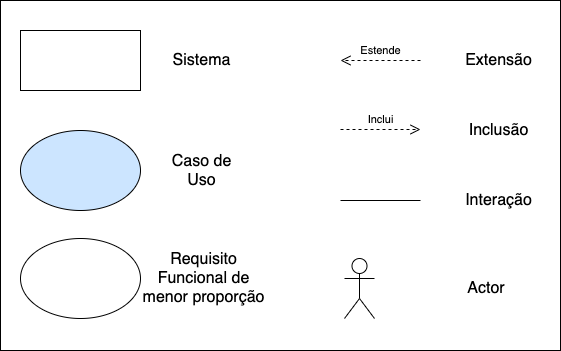
\includegraphics[width=0.7\textwidth]{img/rf/legenda}
		\caption{Legenda dos diagramas}
		\label{fig:rf-legenda}
	\end{center}
\end{figure}

Numa segunda fase serão analisados os graus de prioridade de cada requisito, consoante a sua importância para o projeto e por fim será feita uma descrição detalhada (i. e. especificação do requisito) de cada requisito através de casos de uso. É de notar que parte do grande trabalho da análise do grau de prioridade dos requisitos será imediato devido às decisões por parte do cliente.

Desta forma será claro para o leitor, em especial para a equipa de desenvolvimento, o comportamento que o sistema terá de cumprir. Os casos de uso serão detalhados consoante a seguinte estrutura:

\begin{itemize}
	\item \textbf{ID:} ID do caso de uso.
	\item \textbf{Ator:} Responsável pela realização do caso de uso.
	\item \textbf{Prioridade:} Representa a prioridade do caso de uso baseada nas decisões do cliente, visão dos stakeholders e no funcionamento do sistema. As prioridades foram classificadas por:
	\begin{itemize}
		\item \textbf{\textit{Must Have}:} Como o próprio nome indica, os requisitos \textit{Must} são os requisitos com maior prioridade. \textit{"As a rule, product inception depends entirely on defining must-haves using such pointers as ‘required for launch’, ‘required for safety’, ‘required for validation’, ‘required to deliver a viable solution’, etc."}\cite{moscow}. Todos os requisitos categorizados como \textit{Must Have}, são mandatórios para a equipa de desenvolvimento visto que sem eles o projeto fica paralisado.\textit{ "Can we move forward with the project if this task is undone? – if \textbf{NO}, it’s \textbf{MUST}"}\cite{moscow}.
		\item \textbf{\textit{Should Have}:} Os requisitos \textit{Should} são requisitos que também têm uma elevada prioridade, ou por outras palavras, estão apenas um passo abaixo dos requisitos \textit{Must} .
		Não são requisitos considerados vitais contudo adicionam valor significativo.\textit{ "Will we move forward with the project if this task is done a bit later? – if \textbf{YES}, it’s \textbf{SHOULD}"}\cite{moscow}.
		\item \textbf{\textit{Could Have}:} Os requisitos \textit{Could} são requisitos com menos importancia e impacto que os anteriores. Pode-se dizer, por outras palavras, que são requisitos \textit{Nice to have} e tipicamente só são implementados se houver tempo para tal. \textit{ "Can we sacrifice this task till deadline? – if \textbf{YES}, it’s \textbf{COULD}"}\cite{moscow}.
		\item \textbf{\textit{Won't Have}:} Os requisitos \textit{Won't} são os requisitos com menor prioridade. Os requisitos categorizados com esta prioridade, tipicamente não são implementados no tempo estipulado para o projeto. Alguns requisitos são priorizados no futuro, outros nunca chegam a ser implementados. \textit{ "Can we back to it when things go better? – if \textbf{YES}, it’s \textbf{WON’T}"}\cite{moscow}.
	\end{itemize}
	\item \textbf{Descrição:} Uma breve contextualização do caso de uso.
	\item \textbf{Pré-condições:} Conjunto de condições necessárias para realizar o caso de uso.
	\item \textbf{Estímulo:} Casos de uso responsáveis pela ativação do caso de uso.
	\item \textbf{Fluxo Principal:} Descrição detalhada de todos os passos para a realização do casos de uso.
	\item \textbf{Fluxo de Excepção:} Descrição detalhada do comportamento do sistema quando o caso de uso não for realizado com sucesso.
	\item \textbf{Observações:} Observações adicionais, relevantes para o desfecho do caso de uso.
\end{itemize}

\newpage

\subsection{Diagrama de contexto}
\label{d:contexto}
\begin{figure}[ht!]
	\begin{center}
		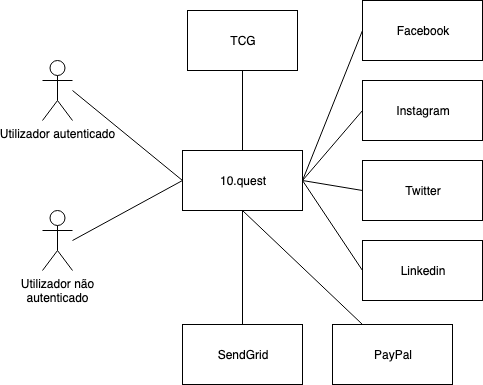
\includegraphics[width=0.6\textwidth]{img/rf/10quest}
		\caption{Diagrama de contexto}
		\label{fig:rf-10quest}
	\end{center}
\end{figure}

A 10.quest, tal como referido nos capítulos anteriores, é uma plataforma de inbound marketing que permite aos utilizadores criar formações, questionários, concursos e tratar a informação recolhida por cada um destes componentes. 
Estes componentes poderão ser partilhados nas redes sociais (i. e. utilizando a API do Facebook, Instagram, Twitter e LinkedIn) através de \textit{landing pages}. Estas \textit{landing pages} terão um pequeno formulário que necessita das informações básicas ao utilizador final para que, automaticamente, as formações, questionários e concursos sejam enviados por mail para os inscritos, utilizando o sistema externo SendGrid.

Tal como referido no Capítulo \ref{sec:estado-arte}, o \acrshort{tcg} é um produto desenvolvido pela 10.digital e actualmente no mercado. Algumas das funcionalidades fundamentais da plataforma a desenvolver já estão implementadas no \acrshort{tcg}  e por isso mesmo haverá uma interação com o mesmo para aproveitar todas estas funcionalidades necessárias.


\newpage

\subsection{Diagrama de alto nível}
\label{d:altonivel}
\begin{figure}[ht!]
	\begin{center}
		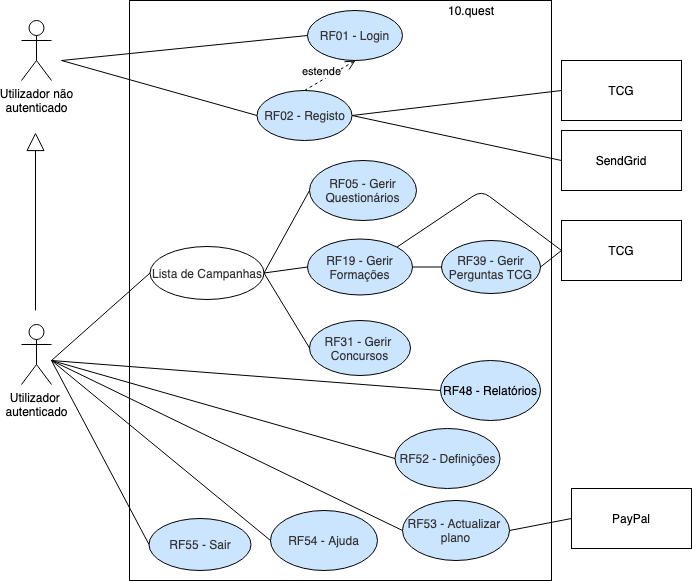
\includegraphics[width=0.8\textwidth]{img/rf/alto-nivel}
		\caption{Diagrama de Alto Nível}
		\label{fig:rf-alto-nivel}
	\end{center}
\end{figure}

Um utilizador para aceder a todas as funcionalidades da plataforma terá de primeiro realizar a autenticação ()\textbf{RF - Registo}). Caso ainda não tenha uma conta registada terá de o fazer. Assim que a conta for criada é enviada uma notificação para o email do utilizador, recorrendo ao sistema externo SendGrid. Por questões de segurança e confidencialidade dos dados, no acto do registo, a informação do utilizador será enviada e guardada na base de dados do \acrshort{tcg}, para que mais tarde todos os pedidos REST possam ser validados.

Depois de um utilizador se autenticar, será direcionado para a página inicial. A partir daqui o utilizador conseguirá gerir questionários, formações, concursos e perguntas para as formações do \acrshort{tcg}; aceder às definições, actualizar o plano da conta, utilizar o suporte da plataforma e terminar sessão.
Ainda na página inicial da plataforma serão exibidas algumas estatísticas relacionadas com as formações, questionários e concursos associados à conta do utilizador. 

\newpage

\subsection{Diagrama Registo}
\label{d:registo}
\begin{figure}[ht!]
	\begin{center}
		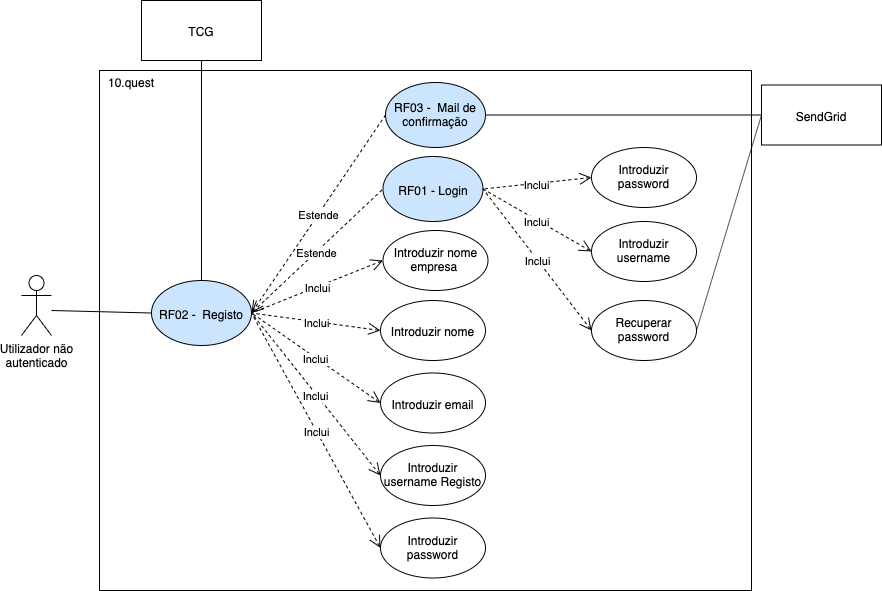
\includegraphics[width=1\textwidth]{img/rf/registo}
		\caption{Diagrama Gerir Concursos}
		\label{fig:rf-registo}
	\end{center}
\end{figure}

Para se efectuar um registo é necessário introduzir o nome da empresa, nome do utilizador, email, \textit{username} e \textit{password}. De seguida o utilizador é direcionado para a página de login onde terá de introduzir o \textit{username} e \textit{password} para se autenticar.

Depois de se efectuar um registo é enviado um mail de confirmação para o email associado à conta.

\newpage

\subsection{Diagrama Gerir Perguntas TCG}
\label{d:perguntastcg}
\begin{figure}[ht!]
	\begin{center}
		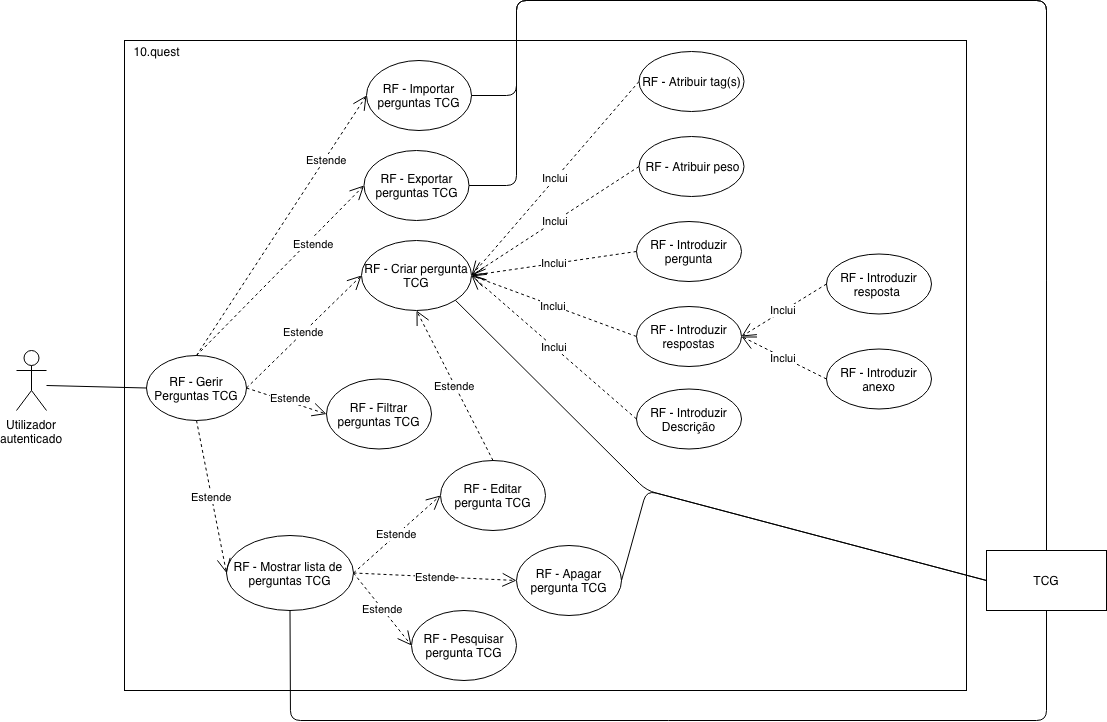
\includegraphics[width=1\textwidth]{img/rf/gerir-perguntas-tcg}
		\caption{Diagrama Gerir Perguntas TCG}
		\label{fig:rf-gerir-perguntas-tcg}
	\end{center}
\end{figure}

No \acrshort{tcg}, tal como referido no Capítulo \ref{sec:TCG}, a criação de questões é isolada da criação de formulários. Dito isto é necessário criar questões para que se possa ter conteúdos para as formações. 

Aproveitando as funcionalidades do \acrshort{tcg} e  tendo em conta que esta abordagem traz uma serie de vantagens, referidas no Capítulo \ref{sec:TCG}, a plataforma a desenvolver irá seguir o mesmo modelo. 

É ainda de notar que por uma questão de terminologia, na plataforma a desenvolver, as Perguntas TCG são equivalentes às questões no \acrshort{tcg}, pelo simples facto de não se confundir com elementos relacionados com os questionários.

Na gestão de Perguntas TCG, um utilizador consegue listar todas as perguntas (\textbf{RF45 - Mostrar lista de perguntas TCG}) associadas à sua conta (i. e. criadas por ele) e pode também criar uma nova pergunta (\textbf{RF42 - Criar pergunta TCG}). O sistema efetua um pedido de todas essas perguntas ao \acrshort{tcg} e a partir daqui o utilizador consegue criar, eliminar (\textbf{RF47 - Apagar pergunta TCG}), editar (\textbf{RF46 - Editar pergunta TCG}) e pesquisar perguntas. As perguntas podem também ser importados e exportados através de uma \textit{spreadsheet}.

Para um criar uma pergunta (\textbf{RF42}), o utilizador precisa de atribuir uma tag, nova ou existente, e introduzir a pergunta, as respostas e uma descrição, sendo esta última opcional. Cada pergunta tem que ter pelos menos duas respostas sendo estas compostas pela resposta e um anexo opcional que pode ser um ficheiro de som, imagem ou vídeo.



\newpage

\subsection{Diagrama Gerir Formações}
\label{d:formacoes}
\begin{figure}[ht!]
	\begin{center}
		\includegraphics[width=1\textwidth]{img/rf/gerir-formacoes}
		\caption{Diagrama Gerir Formações}
		\label{fig:rf-gerir-formacoes}
	\end{center}
\end{figure}

Praticamente todas as funcionalidades da gestão de formações já estão implementadas no \acrshort{tcg} por isso, muitas das funcionalidades irão recorrer à capacidade do \acrshort{tcg} através de pedidos REST e toda a informação relacionada com formações será também guardada na base de dados do \acrshort{tcg}.

Na gestão de formações um utilizador consegue listar todas as formações associadas à sua conta (\textbf{RF27 - Mostrar lista de formações do utilizador}) e pode também criar uma nova formação (\textbf{RF20 - Criar formação}). O sistema efetua um pedido de todas essas formações ao \acrshort{tcg} e a partir daqui o utilizador consegue criar, eliminar, editar e pesquisar formações.

Para criar uma formação (\textbf{RF20}) o utilizador terá, numa primeira instância, de atribuir um nome e definir a periodicidade (i. e. preencher a data de início e fim, dias da semana, hora de envio e  duração/validade) (\textbf{RF21 - Definir periodicidade}). 

Numa segunda fase, o utilizador, através do requisito \textbf{RF - Definições da formação} consegue adicionar e gerir entradas (\textbf{RF25 - Adicionar entrada de perguntas} e \textbf{RF26 - Gerir entradas de perguntas}, respectivamente). As definições da formação (\textbf{RF24 - Definições da formação}) é onde o utilizar, através de \textit{tags} associa grupos de perguntas a grupos de pessoas. 

Numa entrada o utilizador terá de introduzir a \textit{tag} de utilizador(es), a \textit{tag} da(s) pergunta(s) e o número de perguntas dessa \textit{tag} que serão enviadas em cada \textit{quiz}(i. e. cada iteração) da formação.

Por fim o utilizador pode partilhar a formação (\textbf{RF56 - Partilhar}). As inscrições numa formação serão feitas através de uma \textit{landing page} que pode ser personalizada no requisito \textbf{RF08 - Landing Page} e enviadas para o email introduzido no mini formulário da \textit{landing page}. Este mail com o link para a formação, pode ser personalizado no requisito \textbf{RF09 - Notificações por E-mail}. 

É de notar que, através do requisito \textbf{RF29 - Adicionar novo utilizador final TCG}, sempre que um utilizador final se inscreve numa formação através da \textit{landing page}, o sistema, de forma automática, envia os dados para \acrshort{tcg} para que este utilizador possa começar a receber a formação por email. Outro requisito da responsabilidade do sistema é o \textbf{RF30 - Notificar utilizadores finais TCG}, que respeitando a periodicidade definida na criação do formação, envia a formação para todos os inscritos.



\subsection{Diagrama Gerir Questionários}
\label{d:quests}
\begin{figure}[ht!]
	\begin{center}
		\includegraphics[width=1\textwidth]{img/rf/gerir-quest}
		\caption{Diagrama Gerir Questionários}
		\label{fig:rf-gerir-quest}
	\end{center}
\end{figure}

Na gestão de questionários, à semelhança da gestão de formações, é feita uma listagem dos questionários (\textbf{RF15 - Mostrar lista de questionários do utilizador}) e o utilizador tem a capacidade de criar (\textbf{RF06 - Criar questionário}), eliminar, editar (\textbf{RF16 - Editar questionário}) e pesquisar questionários.

Na criação de um novo questionário (\textbf{RF06}), um utilizador, numa primeira fase terá de criar um conjunto de questões (\textbf{RF10 - Criar questões}) e gerar um série de resultados (\textbf{RF11 - Criar resultados}). Cada resultado terá de ter obrigatoriamente uma \textit{tag} associada e um título e caso o utilizador deseje uma imagem e/ou um link. As perguntas e resultados podem também ser importados e exportados numa \textit{spreadsheet}.

Depois de terminar a primeira fase, podendo a qualquer momento voltar a essa fase, o utilizador já tem recursos para começar a criar o questionário (i. e. o sistema de pontuação através do requisito \textbf{RF14 - Criar sistema de pontuação}). Numa primeira instância o utilizador terá de selecionar a pergunta pelo qual deseja começar o questionário. De seguida cria uma ou mais respostas e para cada uma delas é necessário associar uma pergunta que na iteração seguinte sejam apresentadas e se possa repetir este processo para conseguir criar um fluxo de perguntas. Para cada pergunta é atribuído um peso e para cada resposta são associadas \textit{tags} de resultados. Desta forma numa dada pergunta, as \textit{tags} da resposta selecionada serão pontuadas. A qualquer momento o utilizador, em vez de associar uma pergunta a uma resposta, pode decidir, naquele estado (i. e. numa resposta em específico), terminar o questionário e apresentar o resultado ao utilizador final.

Através do requisito \textbf{RF18 - Adicionar novo utilizador final}, sempre que um utilizador final se inscreve num questionário através da \textit{landing page}, o sistema, de forma automática, guarda essa informação e recorrendo ao requisito \textbf{RF17 - Notificar utilizadores finais}, enviei o questionário para os utilizador final.


\subsection{Diagrama Gerir Concursos}
\label{d:concursos}
\begin{figure}[ht!]
	\begin{center}
		\includegraphics[width=1\textwidth]{img/rf/gerir-concurso}
		\caption{Diagrama Gerir Concursos}
		\label{fig:rf-gerir-concursos}
	\end{center}
\end{figure}


Na gestão de concursos, à semelhança da gestão de formações e questionários, é feita uma listagem dos concursos (\textbf{RF37 - Mostrar lista de concursos do utilizador}) e o utilizador tem a capacidade de criar (\textbf{RF32 - Criar concurso}), eliminar, editar (\textbf{RF38 - Editar concurso}) e pesquisar questionários.

Na criação de um concurso (\textbf{RF32}) o utilizador terá de criar perguntas (\textbf{RF33 - Criar perguntas}). Para cada pergunta o utilizador terá de introduzir pelo menos duas respostas (\textbf{RF34 - Introduzir respostas}) e caso o desejo pode adicionar um anexo no formato de imagem. As perguntas e respostas podem também ser importados e exportados numa \textit{spreadsheet} (\textbf{RF36 - Importar perguntas} e \textbf{RF35 - Exportar perguntas}, respectivamente).

É importante referenciar que à semelhança da gestão de formações e questionários, é possível editar os conteúdos (i. e. perguntas, questões, \textit{landing pages}, email etc) contudo, assim que um concurso é publicado e passa a estar no estado \textit{online}, as perguntas deixam de poder ser editáveis. 

Os concursos, tal como os questionários têm sempre um estado que pode variar entre:
\begin{itemize}
	\item Rascunho - Utilizador não deu o concurso como concluído.
	\item Aberto - Utilizador deu o concurso como concluído.
	\item \textit{Online} - Utilizador gerou a \textit{landing page} para partilhar o concurso.
	\item Fechado - Concurso chegou à data de fim.
\end{itemize}


\subsection{Diagrama Ajuda}
\label{d:ajuda}
\begin{figure}[ht!]
	\begin{center}
		\includegraphics[width=1\textwidth]{img/rf/ajuda}
		\caption{Diagrama Ajuda}
		\label{fig:rf-ajuda}
	\end{center}
\end{figure}


O utilizador poderá, se assim o pretender, utilizar o suporte da plataforma. Em caso de dúvida ou esclarecimentos, enviar uma mensagem direta para a 10.digital. 

Para enviar uma mensagem é necessário introduzir o nome, email, mensagem e, caso o utilizador deseje, um ou mais anexos.

\newpage

\subsection{Diagrama Relatórios}

\begin{figure}[ht!]
	\begin{center}
		\includegraphics[width=1\textwidth]{img/rf/relatorio}
		\caption{Diagrama Relatórios}
		\label{fig:rf-relatorios}
	\end{center}
\end{figure}

Assim que uma formação, questionário ou concurso terminar, ou a qualquer momento, um utilizador pode gerar o relatório de dados. A secção de dados da plataforma mostra os resultados gerais sobre as formações questionários e concursos (\textbf{RF49 - Relatório geral}). 

O utilizador pode gerar um relatório (\textbf{RF50 - Relatório}) para um questionário onde será exposto o resultados do mesmo. Será mostrado um gráfico de conversão de tipos de utilizadores finais e uma secção onde se pode calcular a taxa de conversão. Serão também mostrados os resultados do questionário e as respostas por pergunta. Pode ser ainda visto no final um gráfico temporal de eventos.

Para os relatórios de concursos será exposto uma tabela com as classificações de cada participante e para os relatórios de uma formação será feito um pedido ao TCG para retornar o relatório relativo à formação selecionada.

Por fim, na secção de dados (i. e. relatórios) o utilizador pode navegar a lista de leads (\textbf{RF51 - Listar Leads por perfil}) que vão participando nas suas formações, questionários e concursos. Esta lista terá todos os utilizadores finais listados que são considerados leads e é possível filtrar os mesmos por tags (i. e. criar um perfil de utilizador). Para cada utilizador serão apresentados os dados pessoais que eles vão fornecendo ao longo da jornada (e. g. nome, email etc...)




\section{Mockups}
\label{prototipagem}

A criação de mockups/protótipos de baixa fidelidade, teve como principal objetivo representar a plataforma (i. e. todos os requisitos funcionais) de forma estática. Esta secção foi importante para conseguir visualizar a plataforma como um todo, facilitando a implementação, e também teve um papel importante na verificação dos requisitos levantados, satisfazendo todos os casos de uso descritos no Anexo \ref{a:cu}. Todos os mockups realizados encontram-se descritos no Anexo \ref{a:prototipos}.


%-------------------------------------------------------------------------------------------------
\blankpage
%-------------------------------------------------------------------------------------------------

\glsresetall

\chapter{Arquitetura}
\label{sec:arquitetura}

A arquitectura é uma etapa fundamental em todos os projetos porque é aqui que se define a estrutura e comportamento do sistema na sua globalidade e nas diferentes componentes.

Neste capítulo está exposta a arquitetura do 10.quest que servirá de \textit{guideline} para a implementação do projeto. Serão apresentadas diferentes perspetivas para analisar os diferentes aspetos do sistema. É de notar que as componentes a desenvolver pela restante equipa de desenvolvimento não serão analisadas e apenas serão apresentadas de forma superficial para fazer a ligação às componentes a desenvolver no âmbito do estágio curricular.
Este capítulo é também uma exposição das decisões arquiteturais efectuadas no primeiro semestre, respeitando as restrições técnicas e de negócios.

Por fim será feita uma análise dos riscos envolvidos no desenvolvimento do projecto, o seu impacto e probabilidade de ocorrência e o respectivo plano de mitigação




\section{Análise da Arquitetura}
\label{analisearq}

Na análise da arquitetura serão apresentadas as restrições do projecto, que têm um impacto directo nas decisões de arquitetura, nas diferentes perspetivas de arquitetura e nas tecnologias utilizadas.

\subsection{Restrições Técnicas}
As restrições técnicas são decisões técnicas arquiteturais que devem ser satisfeitas. O Sistema a desenvolver deve respeitar as seguintes restrições:

\textbf{Identificador: RT01}
\newline
\textbf{Título:} Arquitectura REST
\newline
\textbf{Descrição:} A comunicação entre a plataforma a desenvolver e o TCG deve seguir uma arquitetura REST.

\textbf{Identificador: RT02}
\newline
\textbf{Título:} Base de Dados
\newline
\textbf{Descrição:} Os dados utilizados pela aplicação devem ser guardados numa base de dados, visto tratar-se de um grande volume de dados que tem de permanecer organizado. Relativamente aos dados do TCG foi imposto que os dados não sejam duplicados e que esta informação seja acedida através de pedidos \acrshort{https}/\acrshort{rest}. PostgreSQL\cite{sql} é a base de dados relacional utilizada pela empresa e portanto será também utilizada no desenvolvimento deste projecto.

\textbf{Identificador: RT03}
\newline
\textbf{Título:} Framework Django\cite{django}
\newline
\textbf{Descrição:} A Framework Django é a técnologia utilizada pela empresa para desenvolver aplicações \textit{web} e \textit{\acrshort{saas}}. O uso desta tecnologia foi imposta pelo \textit{Product Owner}.

\textbf{Identificador: RT04}
\newline
\textbf{Título:} Plataforma Web
\newline
\textbf{Descrição:} Todas as funcionalidades do sistema devem estar disponíveis através da plataforma web.

\subsection{Restrições de Negócio}
Nesta secção estão descritas as restrições de negócio, que podem ser entendidas como barreiras pelas quais a organização deve lutar para executar a sua estratégia. Estas restrições, que apresento em seguida foram impostas pelo \textit{Product Owner} e devem ser satisfeitas na arquitectura do sistema:

\textbf{Identificador: RN01}
\newline
\textbf{Título:} Programa de Desenvolvimento
\newline
\textbf{Descrição:} O produto deve estar concluído e validado até dia 15 de Junho.



\subsection{\acrfull{mvc}}

A estrutura de um projeto Django é muitas vezes descrito como um projeto \acrshort{mvc}. Como podemos ver na Figura \ref{fig:arq-mvc}, o modelo \acrshort{mvc} é uma arquitectura de software que separa a aplicação em três componentes lógicos principais. Por outras palavras este modelo separa a apresentação dos dados, da lógica que trata das \textit{interfaces} do utilizador, facilitando a programação das diferentes funcionalidades, \textit{debugging} e os testes das mesmas.

\begin{figure}[ht!]
	\begin{center}
		\includegraphics[width=1\textwidth]{img/arq/diagrama-MVC}
		\caption{Estrutura do Sistema}
		\label{fig:arq-mvc}
	\end{center}
\end{figure}

O componente \textbf{Model} controla a organização e armazenamento dos dados. Este módulo representa os dados que são transferidos entre os componentes Controller e View mas não representa nenhuma lógica no que diz respeito ao que é representado na camada de apresentação.

O componente \textbf{View} pode ser considerada a camada de apresentação. Este componente contém todas os ingredientes que constituem as interfaces do utilizador e controla a forma como a informação lhe é apresentada. Este modelo sabe como aceder ao modelo de dados que é apresentado ao utilizador contudo não sabe como o manipular nem o que significa.

Por último temos o componente \textbf{Controller}.  Este componente atua entre os modelos View e Model reagindo a eventos na View e respondendo a estes pedidos manipulando os dados utilizando o componente Model e interagindo com o componente View para renderizar o \textit{output}.


\subsection{Modelo C4}

Nesta secção encontra-se representada e descrita toda a arquitetura da plataforma 10.quest,  influenciada pelos objetivos de negócio, \textit{stakeholders}, requisitos e restrições técnica e de negócio, apresentados anteriormente.

Foram utilizados três diagramas para representar a arquitetura do sistema, utilizando o \textbf{modelo C4}\cite{c4}: diagrama de contexto, diagrama de contentores, diagrama de componentes e o diagrama de classes.

Os diferentes diagramas representam diferentes perspetivas e níveis de abstração e foram feitos com o intuito de facilitar a compreensão da arquitetura permitindo à equipa de desenvolvimento visualizar os diferentes níveis de granularidade. 

O diagrama de contexto mostra a relação entre o sistema que vai ser desenvolvido e outros agentes como, por exemplo, utilizadores e sistemas externos.  Este é o diagrama com maior nível de abstração e é bom para sublinhar as dependências externas que a equipa de desenvolvimento tem que integrar no sistema. 

O diagrama de contentores apresenta um maior detalhe (i. e. relativamente ao diagrama de contexto) e mostra os diferentes contentores que constituem o sistema (e. g. bases de dados, aplicações, microserviços etc...). Neste diagrama são também definidas algumas decisões arquiteturais. 

Por último temos o diagrama de componentes que aproxima um contentor individualmente e mostra todos os componentes que constituem esse contentor. Desta forma conseguimos perceber as principais funcionalidades do sistema. 


\subsubsection{Diagrama de Contexto}

Como foi referido no Capítulo \ref{sec:introducao} o 10.quest é uma plataforma de inbound marketing que consiste num \textit{backoffice} para criação de questionários, concursos e criação de formulário com o auxílio do \acrshort{tcg}.

Como podemos ver na Figura \ref{fig:arq-contexto} o 10.quest interage com seis sistemas externos. O SendGrid\cite{sg} é um \acrshort{saas}, na \textit{cloud}, que fornece um serviço de entrega de emails. Este serviço permite enviar emails através de APIs flexíveis garantindo uma disponibilidade  de 99.999\% \cite{sguptime}. 
O TCG, tal como foi referido no Capítulo \ref{sec:estado-arte}, é uma plataforma de criação de formações que tem como principal objectivo, transmitir conhecimento através de uma técnica de aprendizagem baseada em tentativa e erro Algumas das funcionalidades do \acrshort{tcg} serão utilizadas pelo 10.quest.
Para partilhar os questionários, concursos e formações o 10.quest irá utilizar as APIs do Facebook, LinkedIn, Twitter e Instagram.


\newpage

\begin{figure}[ht!]
	\begin{center}
		\includegraphics[width=0.9\textwidth]{img/arq/diagrama-contexto}
		\caption{Diagrama de Contexto}
		\label{fig:arq-contexto}
	\end{center}
\end{figure}

\subsubsection{Diagrama de Contentores}

Na Figura \ref{fig:arq-contentores} está representado o diagrama de contentores, onde se pode observar com mais detalhe a constituição do sistema de software.

Os utilizadores podem ser de dois tipos: o utilizador do backoffice que tem acesso a todas as funcionalidade da plataforma e o utilizador final que tem acesso a uma página web para participar nas formações, concursos e ou questionários.

A aplicação web efetua os pedidos dos utilizadores, através de pedidos \acrshort{https}/\acrshort{rest} à API. A aplicação web será a camada de apresentação da API e ambos serão desenvolvidos em Django. A API será o contentor responsável por tratar de todos os pedidos efetuados pelos utilizadores do \textit{backoffice}. Para este efeito a API implementa um conjunto de funcionalidades, representadas na Figura \ref{fig:arq-componentes1}, que manipulam um conjunto de dados armazenados numa base de dados relacional PostgreSQL, para conseguir as informações necessárias.
\newpage

\begin{figure}[ht!]
	\begin{center}
		\includegraphics[width=0.9\textwidth]{img/arq/diagrama-contentores}
		\caption{Diagrama de Contentores}
		\label{fig:arq-contentores}
	\end{center}
\end{figure}

\subsubsection{Diagrama de Componentes}

Na Figura \ref{fig:arq-componentes} é apresentado o diagrama de componentes e na Figura \ref{fig:arq-componentes1} são apresentados os componentes da API. 

A autenticação é necessária para que os pedidos sejam aceites e mapeados pela API. Para isto a componente "Autenticação", permite ao utilizador efetuar a sua autenticação e verifica a autenticidade do mesmo, em cada pedido, através de tokens. Desta forma, caso o utilizador esteja autenticado os seus pedidos \acrshort{https}/\acrshort{rest} avançam para a componente API , que inclui todas as componente (i. e. funcionalidades) que dão resposta aos requisitos funcionais definidos para o projeto.

A componente "Dados" permite às restantes componentes interagir com a base de dados, tanto para ler, como para escrever.


\begin{figure}[ht!]
	\begin{center}
		\includegraphics[width=0.86\textwidth]{img/arq/diagrama-componentes}
		\caption{Diagrama de Componentes}
		\label{fig:arq-componentes}
	\end{center}
\end{figure}

\begin{figure}[ht!]
	\begin{center}
		\includegraphics[width=0.87\textwidth]{img/arq/diagrama-componentes1}
		\caption{Diagrama Componentes da componente Funcionalidades}
		\label{fig:arq-componentes1}
	\end{center}
\end{figure}

\newpage

%\subsection{Modelo Sequencial}

%\subsection{Modelo de Dados}


%  FALTA CAPITULO PARA DISCUSSÂO VALIDAÇÂO DA ARQUITECTURA. Escrever assim que todas as decisões estiveres feitas

\subsection{Tecnologias Utilizadas}

Grande parte das tecnologias ainda estão por definir. 

\section{Análise de Riscos}
\label{analiseriscos}

Antes de se inicializar a fase de desenvolvimento do projeto é importante realizar uma análise aos possíveis riscos associados ao projeto. Desta forma é importante antecipar/identificar os diferentes riscos que contribuem para o insucesso do projeto para que se possam criar estratégias de mitigação de maneira a minimizar o impacto de cada risco. Os diferentes riscos serão classificados tendo em conta o seu impacto e a sua probabilidade.

\begin{itemize}
	\item[--] \textbf{Probabilidade}
		\subitem \textbf{Baixa}: Menor que 30\%
		\subitem \textbf{Média}: Entre 30\% a 70\%
		\subitem \textbf{Alta}: Superior a 70\%
	\item[--] \textbf{Impacto}
		\subitem \textbf{Baixo}: Interfere no desenvolvimento do projecto.
		\subitem \textbf{Médio}: Interfere no desenvolvimento do projecto e força alterações no produto final.
		\subitem \textbf{Alto}: Compromete a finalização do projeto.
\end{itemize}

De seguida serão listados todos os riscos associados ao projeto e respectivo plano de mitigação para tentar reduzir o impacto do mesmo:

\textbf{R01 - Dependência de sistemas externos}
\begin{itemize}
	\item[--] \textbf{ID}: R01
	\item[--] \textbf{Descrição}: Não se pode garantir uma disponibilidade de 100\% em todos os sistemas externos (e. g. APIs offline) sendo que em algumas ocasiões o sistema pode ter algumas funcionalidades indisponíveis.
	\item[--] \textbf{Estratégia de Mitigação}: Quando um serviço externo está temporariamente indisponível, apesar algumas funcionalidades também indisponíveis, o sistema deve tratar os pedidos do utilizador de forma a afetar a experiência do utilizador, ou no pior dos casos para reduzir o impacto no mesmo.
	\item[--] \textbf{Probabilidade}: Baixa
	\item[--] \textbf{Impacto}: Baixo
\end{itemize}

\textbf{R02 - Dificuldade em implementar o sistema de pagamento}
\begin{itemize}
	\item[--] \textbf{ID}: R02
	\item[--] \textbf{Descrição}: A falta de experiência por parte do aluno na implementação de métodos ou serviços de pagamentos põe em causa a boa implementação do mesmo e pode comprometer uma das principais funcionalidades do produto final.
	\item[--] \textbf{Estratégia de Mitigação}: Deve ser feita uma análise cuidada dos métodos ou serviços de pagamentos disponíveis para integrar com a tecnologia de desenvolvimento da plataforma e de seguida deve ser lida a documentação com atenção para garantir uma boa implementação da mesma.
	\item[--] \textbf{Probabilidade}: Alta
	\item[--] \textbf{Impacto}: Alto
\end{itemize}

\textbf{R03 - Adaptação a novas tecnologias }
\begin{itemize}
	\item[--] \textbf{ID}: R03
	\item[--] \textbf{Descrição}: A não familiarização, por parte do aluno, com as principais tecnologias que irão ser utilizadas na desenvolvimento do projeto, pode criar atrasos implementação devido à falta de experiência e/ou subestimação do tempo definido para cada tarefa, comprometendo a implementação de algumas funcionalidades.
	\item[--] \textbf{Estratégia de Mitigação}: Para além das horas definidas no planeamento do projeto, o aluno terá de dispensar horas extra de modo a conseguir concluir a implementação e validação de todas as funcionalidades.
	\item[--] \textbf{Probabilidade}: Média
	\item[--] \textbf{Impacto}: Médio
\end{itemize}

\textbf{R04 - Novo requisito funcional}
\begin{itemize}
	\item[--] \textbf{ID}: R04
	\item[--] \textbf{Descrição}: As necessidades do cliente podem mudar com o tempo e nesse sentido é possível o aparecimento de um novo requisito funcional.
	\item[--] \textbf{Estratégia de Mitigação}: Reavaliação do plano de desenvolvimento e reestruturação de algumas funcionalidades para que fiquem mais genéricas e assim possa haver tempo para a realização do(s) novo(s) requisito(s). Em alternativa poderão também ter que ser dispensadas algumas horas pelo aluno de modo a cumprir com o plano de desenvolvimento.
	\item[--] \textbf{Probabilidade}: Baixa 
	\item[--] \textbf{Impacto}: Médio
\end{itemize}

Para uma melhor compreensão e visualização dos riscos associados ao projecto será apresentado de seguida, na Tabela \ref{tab:riscos}, um resumo da probabilidade e o impacto de cada risco.

\pagebreak
\mbox{}
\begin{table}
	\centering
\begin{tabular}{ | l | l | l | l |}
	\hline
	\diagbox[width=15em]{Impacto}{Probabilidade}
	& Baixo & Médio & Alto\\
	\hline
	Baixa & \cellcolor{green}\centering R01 & \cellcolor{yellow}R04& \cellcolor{orange}\\
	\hline
	Média & \cellcolor{yellow} & \cellcolor{orange}R03 & \cellcolor{darkOrange}\\
	\hline
	Alta & \cellcolor{orange} & \cellcolor{darkOrange} & \cellcolor{red}R02\\
	\hline
\end{tabular}
\begin{center}
\caption {Classificação dos riscos associados ao projecto}
\label {tab:riscos}
\end{center}
\end{table}



% Listar os Riscos em que activei a estratégia de mitigação e de seguida voltar a mostrar a tabela actualizada







%-------------------------------------------------------------------------------------------------
\blankpage
%-------------------------------------------------------------------------------------------------

\glsresetall

\chapter{Implementação}
\label{sec:implementacao}


\section{Sprints}
\label{sec:sprints}

\section{Ferramentas Utilizadas}
\label{sec:ferramentas}

\section{Desafios na Implementação}
\label{sec:dificuldades}

\section{Produto Final}
\label{sec:finalPro}

%-------------------------------------------------------------------------------------------------
\blankpage
%-------------------------------------------------------------------------------------------------

\glsresetall

\chapter{Validação}
\label{sec:validacao}



\section{Sprints}
\label{sec:sprints}

\section{Desenvolvimento}
\label{sec:desenvolvimento}
%-------------------------------------------------------------------------------------------------
\blankpage
%-------------------------------------------------------------------------------------------------

\glsresetall

\chapter{Produto Final}
\label{sec:produto-final}

%-------------------------------------------------------------------------------------------------
\blankpage
%-------------------------------------------------------------------------------------------------

\glsresetall

\chapter{Conclusion}
\label{sec:conclusion}


Este documento reflete o trabalho realizado durante o primeiro semestre. Esta foi uma fase de muita pesquisa e documentação, para facilitar as fases posteriores do projeto. 

Durante estes ultimos quatro meses o trabalho incidiu principalmente no estudo de mercado, planeamento, escolha da metodologia de trabalho, especificação de requisitos e especificação da arquitectura.

O estudo de mercado, ou por outras palavras, o estado de arte, permitiu avaliar produtos concorrentes e produtos que apesar de terem propósitos distintos, partilham as mesmas funcionalidades. Este estudo permitiu avaliar os pontos fortes e fracos das plataformas que podem ser concorrentes do 10.quest. Desta forma, este estudo não só ajudou a entender a posição do produto em relação ao mercado mas também ajudou a perceber como melhorar a mesma.

A metodologia de trabalho adoptada foi a metodologia utilizada pela empresa. Esta metodologia ajudou na fase da especificação de requisitos visto que, a meio do semestre surgiram novas funcionalidades para o projeto e rápidamente houve uma adaptação.

A Arquitectura ajudou a realizar algumas decisões, apesar de grande parte das decisões ainda estarem por tomar devido a migração de técnologias na empresa, e ajudou também encontrar alguns riscos que podem vir a surgir durante o desenvolvimento. A antecipação destes riscos ajudou na criação de planos de mitigação e assim evitar algumas barreiras no futuro. 

Durante este primeiro projeto surgiraram algumas dificuldades e foram cometidos alguns erros que provocaram alguns atrasos, contudo estas barreiras foram superadas e resolvidas da melhor forma possível. 




%-------------------------------------------------------------------------------------------------
\blankpage
%-------------------------------------------------------------------------------------------------

\glsresetall



%-------------------------------- Citations with no reference --------------------------
\nocite{neipatel}
\nocite{railsware}

\nocite{pg}
\nocite{impact}
\nocite{hubacademy}

\nocite{gfg}
\nocite{tpmvc}
\nocite{djangobook}

\nocite{ibmc4}
\nocite{corediagrams}
\nocite{infoc4}
%---------------------------------------------------------------------------------------


%\bibliographystyle{unsrt}%Used BibTeX style is unsrt
\pagestyle{refstyle}
\renewcommand{\bibname}{Referências}
\bibliography{references}
%\renewcommand\chaptername{Anexo}
\renewcommand{\appendixtocname}{Anexos}
\renewcommand{\appendixpagename}{Anexos}
\renewcommand{\appendixname}{Anexo}
\addappheadtotoc
\appendixtitletocoff
\blankpage
\pagestyle{plain}
\begin{appendices}
	\blankpage
\chapter{\textit{\gls{pop}}}
\label{a:bvm}

\begin{figure}[ht!]
	\begin{center}
		\includegraphics[width=1\textwidth]{img/bmc}
		\caption{10.quest - \textit{\gls{pop}}}
		\label{10q-bmc}
	\end{center}
\end{figure}

Representado na Figura \ref{10q-bmc} temos todo o modelo de negócio da 10.quest representado numa página.

Na secção dos Participantes estão indicados os membros da equipa e os \textit{stakeholders}, os nomes de cada individuo e respectiva função no projecto. 
 
Na secção dos Objectivos é indicado os objetivos principais do projecto, incluindo as métricas de sucesso. 
 
Na Secção dos Utilizadores, estão listados os utilizadores do produto separados por segmentos. 
 
Nos Beneficios dos Utilizadores é representada a proposta de valor e os benefícios que a plataforma traz para os utilizadores. 
 
Na secção das Actividades está a lista concreta de tarefas e acções que a equipa irá ter que realizar para atingir os objetivos do projecto. Nas Entregas estão indicados os resultados e documentos que terão de ser apresentados aos stakeholders ou ao cliente. 
 
Na secção dos Riscos estão identificados possíveis futuros eventos que podem ter um impacto negativo no sucesso do projecto. 
 
Nas Milestones estão listados os pontos críticos que se enquadram na linha temporal do projedcto. 

Na secção das Restrições estão identificados os limites e os requisitos condicionais que afectam diretamente as entregas, actividades ou até mesmo o projecto num todo. 

Por fim temos a secção do Escopo que indica a amplitudo do projeto a ser incluído para consideração, incluindo o que está fora do projeto.
\chapter{Estado de Arte Detalhado}
\label{a:ea}

\section{SurveyMonkey}
\label{surveyMonkey}

O SurveyMonkey é uma plataforma \acrfull{saas} de criação de formulários online que permite recolher e visualizar informações do público alvo através de formulários.

O SurveyMonkey é uma plataforma que dispões de diversos planos de pagamento, e por isso mesmo, apesar de estar disponível um plano gratuito, tem acesso apenas a algumas das funcionalidades e em cada formulário, no máximo, poderá ter 10 perguntas ou elementos.
É necessário criar conta para aceder às funcionalidades da plataforma, dando a opção de utilizar serviços externos para esse efeito : Facebook\cite{face}, LinkedIn, Google\cite{gaccount} e Microsoft\cite{microsoft}.
No painel principal, como podemos ver na Figura \ref{fig:survey-dashboard} temos acesso rápido aos formulários recentes e a algumas métricas sobre os mesmos. Outra forma será aceder aos formulários do utilizador através da barra de navegação. 


\begin{figure}[ht!]
	\begin{center}
		\includegraphics[width=1\textwidth]{img/sm/survey-dashboard}
		\caption{SurveyMonkey - Painel de Controle }
		\label{fig:survey-dashboard}
	\end{center}
\end{figure}

\newpage

\begin{figure}[ht!]
	\begin{center}
		\includegraphics[width=1\textwidth]{img/sm/survey-form-create}
		\caption{SurveyMonkey - Formulários modelo }
		\label{fig:survey-form-create}
	\end{center}
\end{figure}

Quando se inicializa a criação de um novo formulário, a plataforma dá opção de começar do zero ou de utilizar um formulário modelo como podemos ver na Figura \ref{fig:survey-form-create}. Começando um formulário do zero como podemos ver na Figura \ref{fig:survey-form-banck2}, temos acesso a uma série de funcionalidades que vamos explorar e analisar em seguida.

\begin{figure}[ht!]
	\begin{center}
		\includegraphics[width=1\textwidth]{img/sm/survey-form-bank2}
		\caption{SurveyMonkey -  Perguntas Modelo}
		\label{fig:survey-form-banck2}
	\end{center}
\end{figure}


\begin{figure}[ht!]
	\begin{center}
		\includegraphics[width=1\textwidth]{img/sm/survey-form-bank1}
		\caption{SurveyMonkey - Perguntas Modelo }
		\label{fig:survey-form-banck1}
	\end{center}
\end{figure}

\newpage

São diversos os elementos que se podem adicionar ou arrastar para o formulário (i. e. perguntas, escolha multipla, imagens...) como representado na Figura \ref{fig:surveymonkey-form-element} e há também um banco de perguntas modelo/recomendações já construídas, organizadas por categorias como podemos ver na Figura \ref{fig:survey-form-banck2} e \ref{fig:survey-form-banck1}.


\begin{figure}[ht!]
	\begin{center}
		\includegraphics[width=1\textwidth]{img/sm/surveymonkey-form-element}
		\caption{SurveyMonkey - Elementos }
		\label{fig:surveymonkey-form-element}
	\end{center}
\end{figure}
\newpage

\begin{figure}[ht!]
	\begin{center}
		\includegraphics[height=.35\textheight]{img/sm/surveymonkey-form-opcoes}
		\caption{SurveyMonkey - Opções}
		\label{fig:surveymonkey-form-opcoes}
	\end{center}
\end{figure}

\begin{figure}[ht!]
	\begin{center}
		\begin{minipage}{0.45\textwidth}
			\begin{center}
				\includegraphics[height=.35\textheight]{img/sm/surveymonkey-form-aparencia}
				\caption{SurveyMonkey - Aparência}
				\label{fig:surveymonkey-form-aparencia}
			\end{center}
		\end{minipage}
		\hspace{1cm}
		\begin{minipage}{0.45\textwidth}
			\begin{center}
				\includegraphics[height=.35\textheight]{img/sm/surveymonkey-form-logica}
				\caption{SurveyMonkey - Lógica}
				\label{fig:surveymonkey-form-logica}
			\end{center}
		\end{minipage}
	\end{center}
\end{figure}

O SurveyMonkey permite também realizar algumas operações de personalização do formulário. Nas Figuras \ref{fig:surveymonkey-form-opcoes}, \ref{fig:surveymonkey-form-aparencia} e \ref{fig:surveymonkey-form-logica} estão representaçãs as opções, aparência e lógica do formulário, respetivamente, que permite costumizar formulários ao público alvo. 
Depois de realizado o formulário esta plataforma permite a visualização do mesmo, em diferentes tipos de dispositivos, como se pode ver nas Figuras \ref{fig:surveymonkey-form-test-pc} e \ref{fig:surveymonkey-form-test-phone}, para verificar se tudo está conforme planeado para se poder prosseguir para a recolha de dados. 
\newpage

\begin{figure}[ht!]
	\begin{center}
		\includegraphics[width=1\textwidth]{img/sm/surveymonkey-form-test-pc}
		\caption{SurveyMonkey - Visualização do formulário em computador }
		\label{fig:surveymonkey-form-test-pc}
	\end{center}
\end{figure}

\begin{figure}[ht!]
	\begin{center}
		\includegraphics[width=1\textwidth]{img/sm/surveymonkey-form-test-phone}
		\caption{SurveyMonkey - Visualisação do formulário em smartphone }
		\label{fig:surveymonkey-form-test-phone}
	\end{center}
\end{figure}

Depois de garantir que o formulário foi construido como desejado a plataforma fornece vários meios pelo qual se pode partilhar/enviar o formulário, como listado na Figura \ref{fig:surveymonkey-form-share}.

\newpage

\begin{figure}[ht!]
	\begin{center}
		\includegraphics[width=1\textwidth]{img/sm/surveymonkey-form-share}
		\caption{SurveyMonkey - Metodo de partilha do formulário }
		\label{fig:surveymonkey-form-share}
	\end{center}
\end{figure}

Na analise de resultados, é necessário actualizar a página ou aplicar um filtro para que os gráficos e as estatísticas sejam actualizadas. 
O mesmo se passa na página que pode ser gerada para partilhar o sumário dos dados recolhidos, através do formulário. 
Para aplicar um filtro é necessário escolher o tipo de filtro e os elementos ao qual queremos aplicar o filtro como podemos ver nas Figuras \ref{fig:surveymonkey-form-filtro} e \ref{fig:surveymonkey-form-filtro1}. 


\begin{figure}[ht!]
	\begin{center}
		\includegraphics[width=1\textwidth]{img/sm/surveymonkey-form-filtro}
		\caption{SurveyMonkey - Tipos de Filtros }
		\label{fig:surveymonkey-form-filtro}
	\end{center}
\end{figure}



\begin{figure}[ht!]
	\begin{center}
		\includegraphics[width=1\textwidth]{img/sm/surveymonkey-form-filtro1}
		\caption{SurveyMonkey - Filtro aplicado na pergunta 2 }
		\label{fig:surveymonkey-form-filtro1}
	\end{center}
\end{figure}

Para finalizar a plataforma SurveyMonkey tem ainda uma funcionalidade que, através da representação dos dados numa linha temporal, permite o utilizador perceber as tendências dos dados.

\section{Typeform}
\label{typeform}

O Typeform é uma plataforma \acrshort{saas} de criação de formulários online. É uma empresa que afirma resolver o problema dos formulários e inquéritos aborrecidos e tem também como proposta de valor o facto de conseguir criar formulários e inquéritos sem ter que programar uma única linhad e código. Esta plataforma permite recolher informações do público alvo através de formulários e inquéritos personalizados e no final visualizar estes dados. 

O Typeform disponilibilisa um pacote gratuito, contudo, é necessário criar conta de utilizador, para aceder ás funcionalidades da plataforma. Tanto o registro como o início de sessão pode ser feito através da \acrfull{api} do Google.

Como podemos ver na Figura \ref{fig:tf-dashboard}, no painel de controlo, podemos criar várias áreas de trabalho. Cada área de trabalho é independente e todos os formulários e inquéritos que forem adicionados ao mesmo podem ser partilhados com mais do que uma pessoa.

\clearpage

\begin{figure}[ht!]
	\begin{center}
		\includegraphics[width=1\textwidth]{img/tf/tf-dashboard}
		\caption{Typeform - Painel de Controlo}
		\label{fig:tf-dashboard}
	\end{center}
\end{figure}

Na criação de um formulário ou inquérito, do zero, a plataforma lista uma séria de templates que se podem filtrar por categorias na coluna à esquerda, como se pode observar na Figura \ref{fig:tf-form-create}.

\begin{figure}[ht!]
	\begin{center}
		\includegraphics[width=1\textwidth]{img/tf/tf-form-create}
		\caption{Typeform - Criar Formulário}
		\label{fig:tf-form-create}
	\end{center}
\end{figure}
\newpage

\begin{figure}[ht!]
	\begin{center}
		\includegraphics[width=1\textwidth]{img/tf/tf-question-type}
		\caption{Typeform - Tipos de pergunta}
		\label{fig:tf-question-type}
	\end{center}
\end{figure}

Representado na Figura \ref{fig:tf-question-type} temos os tipos de pergunta que a plataforma permite adicionar no formulário. Estas perguntas podem ser personalizaveis tanto a nível estético como funcional como podemos ver nas Figuras \ref{fig:tf-question-opcoes} e \ref{fig:tf-question-custom}, respectivamente. É também possível criar um tema novo para cada pergunta onde se pode escolher a fonte de texto, imagem de fundo e cores da pergunta, respostas, butões e fundo.

\begin{figure}[ht!]
	\begin{center}
		\includegraphics[width=1\textwidth]{img/tf/tf-question-opcoes}
		\caption{Typeform - Opções da pergunta}
		\label{fig:tf-question-opcoes}
	\end{center}
\end{figure}

\begin{figure}[ht!]
	\begin{center}
		\includegraphics[width=1\textwidth]{img/tf/tf-question-custom}
		\caption{Typeform - Design da pergunta}
		\label{fig:tf-question-custom}
	\end{center}
\end{figure}

A plataforma permite ainda os utilizadores adicionarem lógicas aos seus formulário, como exemplificado na Figura \ref{fig:tf-question-logica} , em que caso a resposta à pergunta 4 seja a especificada, o caminho a tomar será diferente. 



\begin{figure}[ht!]
	\begin{center}
		\includegraphics[width=1\textwidth]{img/tf/tf-question-logica}
		\caption{Typeform - Lógica do formulário}
		\label{fig:tf-question-logica}
	\end{center}
\end{figure}

\newpage

A funcionalidade de visualizar o formulário está disponivel no canto superior direito, no lado esquerdo do botão de publicar, que permite o autor verificar se tudo está feito conforme planeado e assim poder publicar e partilhar.

O Typeform permite também a integração de serviços externos com o formulário, como podemos ver na Figura \ref{fig:tf-question-integration} , em que, por exemplo, utilizando o Google Sheets\cite{googlesheets}, os resultados são exportados directamente para uma \textit{google sheet}


\begin{figure}[ht!]
	\begin{center}
		\includegraphics[width=1\textwidth]{img/tf/tf-question-integration}
		\caption{Typeform - Integração com sistemas externos}
		\label{fig:tf-question-integration}
	\end{center}
\end{figure}

Representado na Figura \ref{fig:tf-question-results} , temos a secção de analise de dados da plataforma onde podemos ver uma sumarização dos dados recebidos ou  analisar todas as respostas uma a uma. É também possível gerar um reportório dos dados recebidos e partilhar com alguém em qualquer fase, por exemplo, de uma campanha, uma vez que o mesmo é actualizado automaticamente com as novas respostas recebidas. 

O Typeform não fornece quaisquer filtros para segmentar os dados, contudo, fora as respostas em si, exibe algumas estatísticas/métricas relacionadas com os dispositivos que foram utilizados para responder aos formulários.


\newpage
\begin{figure}[ht!]
	\begin{center}
		\includegraphics[width=1\textwidth]{img/tf/tf-question-results}
		\caption{Typeform - Analise de resultados}
		\label{fig:tf-question-results}
	\end{center}
\end{figure}

\section{Google Form}
\label{googleform}

O Google Form é uma aplicação de adminstração de inquéritos que está incluída no Google Drive office juntamente com o Google Docs\cite{gdocs}, Google Sheets e Google Slides\cite{gslides}. Esta ferramenta permite recolher informações do público alvo através de formulários e inquéritos personalizados e automaticamente exportar os dados para uma \textit{google sheet}.

Estam aplicação é totalmente gratuita, bastanto apenas criar uma conta Google para poder aceder a todas as funcionalidades da ferramenta.

Representado na Figura \ref{fig:gf-dashboard}, está o painel de controlo da conta de um utilizador, onde o mesmo pode visualizar os formulários com que interagiu recentemente. Por cima dos formulários recentes temos o butão para criar um novo formulário juntamente com alguns \textit{templates}/recomendações de formulários.

\newpage

\begin{figure}[ht!]
	\begin{center}
		\includegraphics[width=1\textwidth]{img/gf/gf-dashboard}
		\caption{Google Form - Painel de Controlo}
		\label{fig:gf-dashboard}
	\end{center}
\end{figure}


\begin{figure}[ht!]
	\begin{center}
		\includegraphics[width=1\textwidth]{img/gf/gf-form-q-type}
		\caption{Google Form - Tipos de perguntas}
		\label{fig:gf-form-q-type}
	\end{center}
\end{figure}

A Figura \ref{fig:gf-form-q-type} demonstra a criação de um formulário do zero. Há vários tipo de perguntas que a aplicação permite adicionar ao formulário e, apesar de se estar a criar um formulário novo, o google form permite importar um ou mais formulários diferentes, ao qual o utilizador tem acesso (i. e. formulários que estão disponíveis na sua área de trabalho), selecionando apenas as perguntas que deseja importar. Como podemos ver nas Figuras \ref{fig:gf-form-import}, \ref{fig:gf-form-import-select} e \ref{fig:gf-form-imported} as perguntas importadas foram colocadas na posição escolhida, que neste caso foi no final do formulário.

\begin{figure}[h!]
	\begin{center}
		\includegraphics[width=1\textwidth]{img/gf/gf-form-import}
		\caption{Google Form - Importar formulário}
		\label{fig:gf-form-import}
	\end{center}
\end{figure}

\begin{figure}[h!]
	\begin{center}
		\includegraphics[width=1\textwidth]{img/gf/gf-form-import-select}
		\caption{Google Form - Selecionar perguntas a importar}
		\label{fig:gf-form-import-select}
	\end{center}
\end{figure}

\begin{figure}[h!]
	\begin{center}
		\includegraphics[width=1\textwidth]{img/gf/gf-form-imported}
		\caption{Google Form - Perguntas importadas}
		\label{fig:gf-form-imported}
	\end{center}
\end{figure}


\begin{figure}[h!]
	\begin{center}
		\includegraphics[width=1\textwidth]{img/gf/gf-form-design}
		\caption{Google Form - Alterar design do formulário}
		\label{fig:gf-form-design}
	\end{center}
\end{figure}

\newpage

Grande parte das plataformas e aplicações,no mercado, de criação de formulários permitem personalizar os formulários, ao gosto do utilizador, e o Google Form não é excepção. A aplicação permite alterar as definições padrão do formulário(Figuras \ref{fig:gf-form-set1}, \ref{fig:gf-form-set2} e \ref{fig:gf-form-set3}) e, apesar de se poder também personalidar o \textit{design} do formulário (\ref{fig:gf-form-design}), apens podemos alterar a cor ou imagem de fundo e fonte de texto.

\begin{figure}[ht!]
	\begin{center}
		\includegraphics[height=.30\textheight]{img/gf/gf-form-set1}
		\caption{Google Form - Opções}
		\label{fig:gf-form-set1}
	\end{center}
\end{figure}

\begin{figure}[ht!]
	\begin{center}
		\begin{minipage}{0.40\textwidth}
			\begin{center}
				\includegraphics[height=.22\textheight]{img/gf/gf-form-set2}
				\caption{Google Form - Opções}
				\label{fig:gf-form-set2}
			\end{center}
		\end{minipage}
		\hspace{2cm}
		\begin{minipage}{0.40\textwidth}
			\begin{center}
				\includegraphics[height=.30\textheight]{img/gf/gf-form-set3}
				\caption{Google Form - Opções}
				\label{fig:gf-form-set3}
			\end{center}
		\end{minipage}
	\end{center}
\end{figure}

Antes de partilhar o formulário, precisamos de verificar se o formulário ficou construido como planeado e para isso a aplicação fornece a funcionalidade: \textit{preview}. O Google Form permite os utilizadores enviarem o formulário através de um link, por email, embebido num pagina web ou partilhando no Facebook ou Tweeter utilizando os botões de partilha rápida.

Na análise de resultados, como podemos ver na Figura \ref{fig:gf-form-results} a aplicação faz uma exibição do resumo das respotas, mostrando alguns gráficos/estatisticas contudo, o utilizador não dispõe de nenhuma funcionalidade que filtra ou segmenta os dados. A unica maneira que o utilizador tem de poder tratar os dados e segmenta-los é, depois de exportar os dados, utilizando o Google Sheets, que já requer algum conhecimento na ferramenta. 

\newpage
\mbox{}

\begin{figure}[ht!]
	\begin{center}
		\includegraphics[width=1\textwidth]{img/gf/gf-form-results}
		\caption{Google Form - Sumério dos resultados obtidos}
		\label{fig:gf-form-results}
	\end{center}
\end{figure}

\section{\acrfull{tcg}}
\label{sec:TCG}

O \acrlong{tcg} é um produto actualmente no mercado, desenvolvido pela equipa da 10.digital, que tem como principal objectivo transformar PDFs numa aprendizagem baseada em tentativa erro. O \acrshort{tcg} nasceu de uma forte convicção de que perder apenas 2 minutos por dia numa formação tentativa erro é uma optima forma de aprender, poupando tempo e dinheiro às empresas. Inicialmente muito focado em formação interna, a equipa do \acrshort{tcg} foi-se apercebendo que existem muitos outros problemas (e. g. Consolidação de procedimentos, \textit{Onboarding} de novos colaboradores, Divulgação da cultura da empresa, Divulgação de informações técnicas a parceiros/clientes ...) para o qual a plataforma tem solução (e. g. Assimilação da cultura de empresa e do espírito das marcas, Simplificação do processo de acolhimento, Redução de custos em reuniões periódicas, Facilidade em divulgar aspectos técnicos, que de outra, forma demorariam mais tempo ...).\cite{tcginfo}

O \acrshort{tcg} é um \acrshort{saas} pago que disponibiliza uma demo de 30 dias. Esta demo permite ao utilizador utilizar todas as funcionalidades da plataforma e, tal como nos planos pagos, disponibiliza ainda um tutorial de como efectuar as actividades chaves.

Este produto permite-nos criar utilizadores finais (i. e. quem irá responder à formação), questões e formaçãos. As questões e os utilizadores finais, são categorizados através de tags, optimizando assim a forma como associamos os mesmos a uma formação nova ou já existente, como veremos em diante.

Como podemos ver na Figura \ref{fig:tcg-homepage} na página inicial, a plataforma expõem algumas estatísticas gerais sobre as formações do utilizador.

\newpage


\begin{figure}[ht!]
	\begin{center}
		\includegraphics[width=1\textwidth]{img/tcg/tcg-homepage.png}
		\caption{The Company Gym - Página Inicial}
		\label{fig:tcg-homepage}
	\end{center}
\end{figure}

\begin{figure}[ht!]
	\begin{center}
		\includegraphics[width=1\textwidth]{img/tcg/tcg-utilizadores.png}
		\caption{The Company Gym - Lista de utilizadores finais}
		\label{fig:tcg-utilizadores}
	\end{center}
\end{figure}

Representado na Figura \ref{fig:tcg-utilizadores} está a lista de utilizadores finais. Para criar um novo utilizador final basta criar no botão "+Adicionar" e introduzir uma(s) tag, nova ou já existente, primeiro e ultimo nome e o e-mail por onde vai receber as formações. Como podemos ver há também um botão que permite importar uma lista de utilizadores finais e exportar a lista de utilizadores finais já adicionados no sistema, numa \textit{spreadsheet}.
\newpage

\begin{figure}[ht!]
	\begin{center}
		\includegraphics[width=1\textwidth]{img/tcg/tcg-questoes.png}
		\caption{The Company Gym - Lista de questões criadas}
		\label{fig:tcg-questoes}
	\end{center}
\end{figure}

\begin{figure}[ht!]
	\begin{center}
		\includegraphics[width=1\textwidth]{img/tcg/tcg-criar-questao.png}
		\caption{The Company Gym - Criar questão}
		\label{fig:tcg-criar-questoes}
	\end{center}
\end{figure}

Na Figura \ref{fig:tcg-questoes} podemos ver que é possível listar todas as questão e filtra-las por \textit{tags} e estado. À semelhança do que acontece com os utilizadores, é também possível importar e exportar questões. Como podemos ver na Figura \ref{fig:tcg-criar-questoes} para criar uma nova questão é necessário atribuir uma(s) \textit{tag}, um peso (i. e. importância), um estado (\textit{draft}, \textit{for aproval} e \textit{aproved}), a questão e pelo menos duas respostas. Alguns alpectos como o anexo (i. e. imagem, video ou fichiero de som) na pergunta e/ou resposta são opcionais. Quando se importa uma serie de pergunas através de uma \textit{spreadsheet} todas as questões automaticamente ficam com estado \textit{draft} e como é de esperar sem anexos. Todas as questões que ficam em estado \textit{for aproval} terão de ser aprovadas pelo gestor de conta.


Nas Figuras \ref{fig:tcg-form}, \ref{fig:tcg-form1} e \ref{fig:tcg-form2} temos todas as fases para a criação de uma formação. Em primeiro lugar, é necessário definir a periocidade da formação.  Depois de escolher o nome é necessário dar um dia para o inicio e o fim da mesma, escolher os dias da semana em que o utilizador final irá receber a formação, a hora do dia a que recebe o mail e a duração (i. e. validade) que o utilizador tem para realizar a formação antes da mesma expirar. É de notar que a o sistema aceita uma duração com um max de horas igual à menor diferença entre os dias da semana escolhidos.

A seleção dos utilizadores finais e das questões faz-se através de tags. Desta forma temos uma forma bastante poderosa de adicionar multiplas questões e ao mesmo tempo escolher exatamente quais as questões que queremos numa formação e sem ter que fazer quaqueis alterações, adicionar e remover questões a qualquer hora. O mesmo se trata para os utilizadores finais. 



\begin{figure}[ht!]
	\begin{center}
		\includegraphics[width=1\textwidth]{img/tcg/tcg-form.png}
		\caption{The Company Gym - Criar Formação (Periodicidade)}
		\label{fig:tcg-form}
	\end{center}
\end{figure}

\newpage


\begin{figure}[ht!]
	\begin{center}
		\includegraphics[width=1\textwidth]{img/tcg/tcg-form1.png}
		\caption{The Company Gym - Criar Formação (Definições)}
		\label{fig:tcg-form1}
	\end{center}
\end{figure}

\begin{figure}[ht!]
	\begin{center}
		\includegraphics[width=1\textwidth]{img/tcg/tcg-form2.png}
		\caption{The Company Gym - Criar Formação (Gerir Utilizadores e Questões)}
		\label{fig:tcg-form2}
	\end{center}
\end{figure}

O botão "Activity feed" abre uma nova janela com o histórico de actividades da formação como podemos ver na Figura \ref{fig:tcg-feed}. O historico pode ser organizado pelas caracteristica de cada coluna e para cada registo, é possível ver verificar as respostas do utilizador final na formação.


\begin{figure}[ht!]
	\begin{center}
		\includegraphics[width=1\textwidth]{img/tcg/tcg-feed.png}
		\caption{The Company Gym - Histórico de actividades}
		\label{fig:tcg-feed}
	\end{center}
\end{figure}

\newpage


\begin{figure}[ht!]
	\begin{center}
		\includegraphics[width=1\textwidth]{img/tcg/tcg-tags.png}
		\caption{The Company Gym - Lista de Tags}
		\label{fig:tcg-tags}
	\end{center}
\end{figure}

É também possivel gerir todas as Tags (i. e. adicionar, editar e remover) adicionadas pelo utilizador no sistema como podemos ver na Figura \ref{fig:tcg-tags} e alterar o template do mail que é enviado para os clientes finais com o link para a formação, representado na Figura \ref{fig:tcg-mail}. 

\begin{figure}[ht!]
	\begin{center}
		\includegraphics[width=1\textwidth]{img/tcg/tcg-mail.png}
		\caption{The Company Gym - Alterar template do mail}
		\label{fig:tcg-mail}
	\end{center}
\end{figure}

\newpage

Na analise de resultados, podemos gerar relatórios gerais (i. e. relatórios com estatísticas de todas as formações, questões e utilizadores), como podemos ver na Figura \ref{fig:tcg-data}  e relatórios para uma formação em especifico (i. e. relatórios com estatísticas apenas das formações, questões e utilizadores adicionados a essa formação). 


\begin{figure}[ht!]
	\begin{center}
		\includegraphics[width=1\textwidth]{img/tcg/tcg-data.png}
		\caption{The Company Gym - Relatório geral (Painel inicial)}
		\label{fig:tcg-data}
	\end{center}
\end{figure}

\newpage

\begin{figure}[ht!]
	\begin{center}
		\includegraphics[width=1\textwidth]{img/tcg/tcg-data1.png}
		\caption{The Company Gym - Relatório geral (Participação/Respostas correctas)}
		\label{fig:tcg-data1}
	\end{center}
\end{figure}

Nas Figuras \ref{fig:tcg-data1} e \ref{fig:tcg-data2} temos reprentados a participação/respostas correctas de todas as formações e os resultados globais por formação, respectivamente.

\begin{figure}[ht!]
	\begin{center}
		\includegraphics[width=1\textwidth]{img/tcg/tcg-data2.png}
		\caption{The Company Gym - Relatório geral (Resultados globais por formação)}
		\label{fig:tcg-data2}
	\end{center}
\end{figure}

\newpage


No relatório geral é também possível monitorizar quais as questões com maior numero de respostas erradas e o desempenho de cada utilizador final, como podemos ver nas Figuras \ref{fig:tcg-data3} e \ref{fig:tcg-data4}, respectivamente, numa escala temporal definida pelo utilizador. 

\begin{figure}[ht!]
	\begin{center}
		\includegraphics[width=1\textwidth]{img/tcg/tcg-data3.png}
		\caption{The Company Gym - Relatório geral (\textit{Top} de questões erradas)}
		\label{fig:tcg-data3}
	\end{center}
\end{figure}


\begin{figure}[ht!]
	\begin{center}
		\includegraphics[width=1\textwidth]{img/tcg/tcg-data4.png}
		\caption{The Company Gym - Relatório geral (Utilizadores)}
		\label{fig:tcg-data4}
	\end{center}
\end{figure}

Nos relatórios específicos para uma formação, o tratamento dos dados é muito semelhante como poderemos verificar mais em diante nas Figuras \ref{fig:tcg-data-f},  \ref{fig:tcg-data-f1}, \ref{fig:tcg-data-f2} e \ref{fig:tcg-data-f3}. Depois de selecionar a formação para ser possível gerar o relatório de dados, numa escala temporal definida pelo utilizador, são apresentados os gráficos relativos á percentagem de participação, repostas correctas por \textit{tag} de questão e utilizador. 
No \textit{top} de questões erradas é possível listas os utilizadores finais que erraram uma determinada pergunta. O inverso acontece na página seguinte, representado na Figura \ref{fig:tcg-data-f2}, sendo possível listar as questões onde os utilizadores com mais respostas erradas, erraram. 
Por fim temos a listagem dos utilizadores finais que estão associados à formação em questão, seguidos das estatisticas relacionadas com o seu desempenho.

\begin{figure}[ht!]
	\begin{center}
		\includegraphics[width=1\textwidth]{img/tcg/tcg-data-f.png}
		\caption{The Company Gym - Relatório específico de uma formação (Gráficos)}
		\label{fig:tcg-data-f}
	\end{center}
\end{figure}

\begin{figure}[ht!]
	\begin{center}
		\includegraphics[width=1\textwidth]{img/tcg/tcg-data-f1.png}
		\caption{The Company Gym - Relatório específico de uma formação (\textit{Top} de questões erradas)}
		\label{fig:tcg-data-f1}
	\end{center}
\end{figure}

\begin{figure}[ht!]
	\begin{center}
		\includegraphics[width=1\textwidth]{img/tcg/tcg-data-f2.png}
		\caption{The Company Gym - Relatório específico de uma formação (\textit{Top} de utilizadores com mais respostas erradas)}
		\label{fig:tcg-data-f2}
	\end{center}
\end{figure}

\begin{figure}[ht!]
	\begin{center}
		\includegraphics[width=1\textwidth]{img/tcg/tcg-data-f3.png}
		\caption{The Company Gym - Relatório específico de uma formação (Lista de utilizadores)}
		\label{fig:tcg-data-f3}
	\end{center}
\end{figure}

\newpage
\chapter{Casos de Uso}
\label{a:cu}

\section{Casos de Uso}

\subsection{RF01 - Login}
\begin{itemize}
	\item[--] \textbf{ID:} 01
	\item[--]  \textbf{Ator:} Utilizador.
	\item[--]  \textbf{Prioridade:} \textit{Must have}.
	\item[--]  \textbf{Descrição:} Efectuar .
	\item[--]  \textbf{Pré-condições:} O utilizador necessita de ter uma conta registada na plataforma 10.quest.
	\item[--]  \textbf{Estímulo:} O utilizador deseja efetuar autenticação ou RF02 - Registo.
	\item[--]  \textbf{Fluxo Principal:} 
			\subitem 1. O utilizador deseja entrar na plataforma.
			\subitem 2. O utilizador pressiona o botão de \textit{login}.
			\subitem 3. O utilizador introduz o nome de utilizador e a password.
			\subitem 4. O 10.quest recebe validação das credenciais do utilizador.
			\subitem 5. O 10.quest autentica o utilizador.
			\subitem 6. O 10.quest disponibiliza as funcionalidades para utilizadores autenticados, consoante o plano.
	\item[--]  \textbf{Fluxo de Excepção:} 
			\subitem 4a. As credenciais introduzidas pelo utilizador não correspondem a nenhuma conta registada no sistema.
			\subitem 4a1. O 10.quest informa o utilizador que as credênciais estão incorretas.
\end{itemize}
\newpage

\subsection{RF02 - Registo}
\begin{itemize}
	\item[--] \textbf{ID:} 02
	\item[--]  \textbf{Ator:} Utilizador.
	\item[--]  \textbf{Prioridade:} \textit{Must Have}.
	\item[--]  \textbf{Descrição:} O utilizador efectua o registo na plataforma 10.quest.
	\item[--]  \textbf{Pré-condições:} O utilizador necessita de ter um Email válido.
	\item[--]  \textbf{Estímulo:} O Utilizador deseja criar uma conta na plataforma 10.quest.
	\item[--]  \textbf{Fluxo Principal:} 
		\subitem 1. O utilizador deseja criar conta na plataforma 10.quest.
		\subitem 2. O utilizador pressiona o botão de \textit{sign up}.
		\subitem 3. O utilizador preenche os campos do nome da empresa onde trabalha, nome próprio, email, nome de utilizador e password.
		\subitem 4. O 10.quest recebe validação de que os dados introduzidos são válidos.
		\subitem 5. O 10.quest cria uma nova conta de utilizador.
		\subitem 6. O 10.quest redireciona o utilizador para a página de \textit{login}.
	\item[--]  \textbf{Fluxo de Excepção:} 
			\subitem 4a. O email introduzido pelo utilizador corresponde ao email de uma conta já existente no sistema.
			\subitem 4a1. O 10.quest notifica o utilizador que já existe uma conta registada com o mesmo email que foi introduzido.
	\item[--]  \textbf{Observações:}  O sistema considera os dados válidos se o Email introduzido não correspondem ao Email de uma conta já existente na plataforma 10.quest.
\end{itemize}
\newpage

\subsection{RF03 - Mail de confirmação}
\begin{itemize}
	\item[--] \textbf{ID:} 03
	\item[--]  \textbf{Ator:} 10.quest.
	\item[--]  \textbf{Prioridade:} \textit{Must Have}.
	\item[--]  \textbf{Descrição:} Um utilizador, depois de criar uma conta na plataforma 10.quest, recebe um mail de confirmação.
	\item[--]  \textbf{Pré-condições:} O utilizador cria uma conta nova.
	\item[--]  \textbf{Estímulo:} RF02 - Registo.
	\item[--]  \textbf{Fluxo Principal:} 
			\subitem 1. O 10.quest recebe validação de que os dados introduzidos são válidos.
			\subitem 2. O 10.quest notifica o utilizador que irá receber um mail de confirmação.
\end{itemize}
\newpage


\begin{comment}

\subsection{RF04 - Lista de utilizadores}
\begin{itemize}
	\item[--] \textbf{ID:} 04
	\item[--]  \textbf{Ator:} 
	\item[--]  \textbf{Prioridade:}
	\item[--]  \textbf{Descrição:} 
	\item[--]  \textbf{Pré-condições:} 
	\item[--]  \textbf{Estimulo:}
	\item[--]  \textbf{Fluxo Principal:} 
		\subitem
		\subitem
		\subitem
		\subitem
	\item[--]  \textbf{Fluxo de Excepção:} 
		\subitem
		\subitem
		\subitem
		\subitem
	\item[--]  \textbf{Observações:} 
\end{itemize}
\newpage
\end{comment}

\subsection{RF05 - Gerir Questionários de Personalidade}
\begin{itemize}
	\item[--] \textbf{ID:} 05
	\item[--]  \textbf{Ator:} Utilizador.
	\item[--]  \textbf{Prioridade:} \textit{Must Have}.
	\item[--]  \textbf{Descrição:} O utilizador deseja visualizar, criar, editar ou eliminar um questionário de personalidade.
	\item[--]  \textbf{Pré-condições:} O utilizador necessita de estar autenticado na plataforma 10.quest.
	\item[--]  \textbf{Estímulo:} O utilizador deseja gerir os seus questionários.
	\item[--]  \textbf{Fluxo Principal:} 
		\subitem 1. O utilizador pressiona o botão para entrar na página principal.
		\subitem 2. O 10.quest lista os três tipos de campanhas onde estão \underline{todos os questionários de personalidade do utilizador}.
	\item[--]  \textbf{Fluxo de Excepção:} 
		\subitem 2a. Não existe nenhum questionário de personalidade associado à conta do utilizador.
		\subitem 2a1. o 10.quest informa o utilizador que não existem questionários de personalidade para serem listados.
	\item[--]  \textbf{Observações:} A forma como a platadorma 10.quest lista os questionários está descrito no caso de uso \underline{RF15 - Mostrar lista de questionários de personalidade do utilizador}.
\end{itemize}
\newpage

\subsection{RF06 - Criar Questionário de Personalidade}
\begin{itemize}
	\item[--] \textbf{ID:} 06
	\item[--]  \textbf{Ator:} Utilizador.
	\item[--]  \textbf{Prioridade:} \textit{Must Have}.
	\item[--]  \textbf{Descrição:} O utilizador cria um questionário novo.
	\item[--]  \textbf{Pré-condições:} O utilizador necessita de estar autenticado na plataforma 10.quest.
	\item[--]  \textbf{Estímulo:} RF05 - Gerir Questionários de Pernsonalidade.
	\item[--]  \textbf{Fluxo Principal:} 
		\subitem 1. O utilizador seleciona a opção de criar um novo questionário de personalidade.
		\subitem 2. O 10.quest redireciona o utilizador para a página da criação de um questionário de personalidade onde o utilizador pode efectuar as \underline{operações desejadas}.
	\item[--]  \textbf{Observações:} Depois da plataforma 10.quest redirecionar o utilizador para a página da criação de um questionário de personalidade, este pode efectuar as \underline{operações desejadas}:
	\begin{itemize}
		\item Criar novas questões (RF10 - Criar e editar questões).
		\item Criar resultados (RF11 - Criar e editar resultados).
		\item Importar questões através de uma spreadsheet (RF12 - Importar Questões).
		\item Exportar questões para uma spreadsheet (RF13 - Exportar Questões).
		\item Importar questões através de uma spreadsheet (RF59 - Importar resultados).
		\item Exportar questões para uma spreadsheet (RF58 - Exportar resultados).
		\item Partilhar os questionários de personalidade e/ou definir o template do E-mail (RF07 - Modelo de notificações).
	\end{itemize}
\end{itemize}
\newpage

\subsection{RF07 - Modelo de Notificações}
\begin{itemize}
	\item[--] \textbf{ID:} 07
	\item[--]  \textbf{Ator:} Utilizador.
	\item[--]  \textbf{Prioridade:} \textit{Must Have}.
	\item[--]  \textbf{Descrição:} Secção da plataforma onde se define os templates para a Landing page e para os Emails.
	\item[--]  \textbf{Pré-condições:} O utilizador necessita de estar autenticado na plataforma 10.quest.
	\item[--]  \textbf{Estímulo:}  
		\subitem RF06 - Criar questionário de personalidade.
		\subitem RF16 - Editar questionário de personalidade.
		\subitem RF21 - Definir Periodicidade.
		\subitem RF28 - Editar formação.
		\subitem RF32 - Criar concurso.
		\subitem RF38 - Editar concurso.
	\item[--]  \textbf{Fluxo Principal:} 
		\subitem 1. O utilizador seleciona a secção do Modelo de Notificações.
		\subitem 2. O utilizador efectua as \underline{operações desejadas}.
	\item[--]  \textbf{Observações:} Depois do utilizador se encontrar na secção do modelo e notificações, este pode efectuar as \underline{operações desejadas}:
	\begin{itemize}
		\item Definir o template da Landing Page (RF08 - Landing Page).
		\item Definir o template do Email para ser enviado para os utilizadores finais (RF09 - Notificações por Email).
		\item Partilhar uma campanha (RF56 - Partilhar).
	\end{itemize}
\end{itemize}
\newpage

\subsection{RF08 - Landing Page}
\begin{itemize}
	\item[--] \textbf{ID:} 08
	\item[--]  \textbf{Ator:} Utilizador.
	\item[--]  \textbf{Prioridade:} \textit{Must Have}.
	\item[--]  \textbf{Descrição:} Página de apresentação da campanha para converter um visitante numa lead.
	\item[--]  \textbf{Pré-condições:} O utilizador necessita de estar autenticado na plataforma 10.quest.
	\item[--]  \textbf{Estímulo:} RF07 - Modelo de Notificações.
	\item[--]  \textbf{Fluxo Principal:} 
		\subitem 1. O 10.quest mostra o template da landing page que está definida para o questionário.
		\subitem 2. O utilizador \underline{altera os campos necessários} para a landing page.
		\subitem 3. O utilizador grava as alterações.
		\subitem 4. O 10.quest notifica o utilizador que as alterações foram guardadas com sucesso.
	\item[--]  \textbf{Fluxo de Excepção:} 
		\subitem 3a. O utilizador sai sem gravar as alterações.
		\subitem 3b. O 10.quest não guarda as alterações efectuadas.
	\item[--]  \textbf{Observações:} No lado direito da plataforma é apresentada uma pré-visualização da landing page para ajudar o utilizador a \underline{alterar os campos necessários} e verificar o resultado final:
	\begin{itemize}
		\item Título da landing page.
		\item Texto da landing page (i. e. conteúdo que estará no corpo da landing page).
		\item Imagem ou vídeo para o campanha e imagem da marca, que serão mostrados na landing page.
		\item Cor para a landing page.
	\end{itemize}
	Do lado direito do ecrã será mostrado uma pré-visualização da landing page.
\end{itemize}
\newpage

\subsection{RF09 - Notificações por E-mail}
\begin{itemize}
	\item[--] \textbf{ID:} 09
	\item[--]  \textbf{Ator:} Utilizador.
	\item[--]  \textbf{Prioridade:} \textit{Must Have}.
	\item[--]  \textbf{Descrição:} Template do email que será enviado para os utilizadores finais.
	\item[--]  \textbf{Pré-condições:} O utilizador necessita de estar autenticado na plataforma 10.quest.
	\item[--]  \textbf{Estímulo:} RF07 - Modelo de Notificações.
	\item[--]  \textbf{Fluxo Principal:} 
	\subitem 1. O 10.quest mostra o template do email que está definido para a campanha.
	\subitem 2a. O utilizador seleciona o template pré-definido.
	\subitem 2b. O utilizador seleciona o template personalizado e \underline{alterar os campos necessários}.
	\subitem 3. O utilizador grava as alterações.
	\subitem 4. O 10.quest notifica o utilizador que as alterações foram guardadas com sucesso.
	\item[--]  \textbf{Fluxo de Excepção:} 
	\subitem 3a. O utilizador sai sem gravar as alterações.
	\subitem 3b. O 10.quest não guarda as alterações efectuadas.
	\item[--]  \textbf{Observações:} Caso o utilizador decida utilizar um template personalizado terá de \underline{alterar os campos necessários}:
	\begin{itemize}
		\item Assunto do email.
		\item Texto do email (i. e. conteúdo que estará no corpo do email).
		\item Imagem para o questionário e imagem da marca.
		\item Cor para o template.
	\end{itemize}
	Do lado direito do ecrã será mostrado uma pré-visualização do email.
\end{itemize}
\newpage

\subsection{RF10 - Criar e editar questões}
\begin{itemize}
	\item[--] \textbf{ID:} 10
	\item[--]  \textbf{Ator:} Utilizador.
	\item[--]  \textbf{Prioridade:} \textit{Must Have}
	\item[--]  \textbf{Descrição:} Criar as questões que irão aparecer no questionário de personalidade.
	\item[--]  \textbf{Pré-condições:} O utilizador necessita de estar autenticado na plataforma 10.quest.
	\item[--]  \textbf{Estímulo:}  
		\subitem RF58 - Mostrar lista de questões.
	\item[--]  \textbf{Fluxo Principal:} 
		\subitem 1. O utilizador introduz a questão a ser adicionada ao questionário de personalidade.
		\subitem 2. O utilizador atribui uma pontuação à questão.
		\subitem 3. O utilizador cria pelo menos duas respostas para a pergunta. A cada resposta pode associar uma ou mais tags e uma imagem ou vídeo.
		\subitem 4. O utilizador carrega no botão para adicionar a questão ao questionário de personalidade.
		\subitem 5. O 10.quest notifica o utilizador que a questão foi adicionada com sucesso.
	\item[--]  \textbf{Observações:} O utilizador pode adicionar múltiplas questões ao questionário de personalidade. As questões são adicionadas em formato de lista e por isso para apagar uma questão basta selecionar todas as questões pertendidas e carregar no botão de apagar questões.
\end{itemize}
\newpage

\subsection{RF11 - Criar e editar resultados}
\begin{itemize}
	\item[--] \textbf{ID:} 11
	\item[--]  \textbf{Ator:} Utilizador.
	\item[--]  \textbf{Prioridade:} \textit{Must Have}.
	\item[--]  \textbf{Descrição:} Criar resultados para serem apresentados ao utilizador final.
	\item[--]  \textbf{Pré-condições:} O utilizador necessita de estar autenticado na plataforma 10.quest.
	\item[--]  \textbf{Estímulo:}  
		\subitem RF59 - Mostrar lista de resultados.
	\item[--]  \textbf{Fluxo Principal:} 
		\subitem 1. O utilizador introduz o título para o resultado.
		\subitem 2. O utilizador introduz, opcionalmente, uma descrição para o resultado.
		\subitem 3. O utilizador introduz, opcionalmente, um \textit{link} para o resultado.
		\subitem 4. O utilizador associa uma ou mais tags ao resultado.
		\subitem 5. O utilizador, opcionalmente, carrega uma imagem ou vídeo para o resultado.
	\item[--]  \textbf{Fluxo de Excepção:} 
		\subitem 3a. O utilizador introduz um link inválido.
		\subitem 4a1. O 10.quest notifica o utilizador que o link carregado é inválido.
		\subitem 5a. O utilizador carrega um ficheiro com formato inválido.
		\subitem 5a1. O 10.quest notifica o utilizador que o formato carregado é inválido.
	\item[--]  \textbf{Observações:} 
	A lista de tags disponível para associar ao resultado contém apenas tags criadas nas questões da campanha especifica.
	
	A introdução de um \textit{link}, imagem ou vídeo e tags a um resultado é opcional, contudo sem tags o sistema de pontuação não irá recomendar o respectivo resultado.	
	
\end{itemize}
\newpage

\subsection{RF12 - Importar questões}
\begin{itemize}
	\item[--] \textbf{ID:} 12
	\item[--]  \textbf{Ator:} Utilizador.
	\item[--]  \textbf{Prioridade:} \textit{Must Have}.
	\item[--]  \textbf{Descrição:} Importar questões através de uma spreadsheet. 
	\item[--]  \textbf{Pré-condições:} O utilizador necessita de estar autenticado na plataforma 10.quest.
	\item[--]  \textbf{Estímulo:}  
		\subitem RF58 - Mostrar lista de questões.
	\item[--]  \textbf{Fluxo Principal:} 
		\subitem 1. O utilizador carrega no botão para importar questões.
		\subitem 2. O utilizador carrega a spreadsheet (i. e. ficheiro com as questões) para a plataforma 10.quest.
		\subitem 3. O 10.quest notifica o utilizador que as questões foram adicionadas com sucesso.
	\item[--]  \textbf{Fluxo de Excepção:} 
		\subitem 2a. O utilizador carrega um ficheiro com formato inválido.
		\subitem 2a1. O 10.quest notifica o utilizador que o ficheiro carregado é inválido.
		\subitem 2b. O utilizador carrega um ficheiro mas as questões estão mal formatadas (i. e. mal estruturadas).
		\subitem 2b1. O 10.quest notifica o utilizador quais as questões que estão mal estruturadas e não foram adicionadas ao questionário.
	\item[--]  \textbf{Observações:} É fornecido um ficheiro exemplo para mostrar ao utilizador a estrutura em que as questões têm de ser escritas no ficheiro para ser aceite pela plataforma 10.quest com sucesso.
\end{itemize}
\newpage

\subsection{RF13 - Exportar questões}
\begin{itemize}
	\item[--] \textbf{ID:} 13
	\item[--]  \textbf{Ator:} Utilizador.
	\item[--]  \textbf{Prioridade:} \textit{Must Have}.
	\item[--]  \textbf{Descrição:} Exportar questões para uma spreadsheet.
	\item[--]  \textbf{Pré-condições:} O utilizador necessita de estar autenticado na plataforma 10.quest.
	\item[--]  \textbf{Estímulo:}  
		\subitem RF58 - Mostrar lista de questões.
	\item[--]  \textbf{Fluxo Principal:} 
		\subitem 1. O utilizador carrega no botão para exportar as questões associadas ao questionário de personalidade.
		\subitem 2. O 10.quest descarrega um ficheiro com todas as questões associadas ao questionário de personalidade.
	\item[--]  \textbf{Observações:} Caso não haja questões associadas ao questionário de personalidade, o ficheiro descarregado estará vazio.
\end{itemize}
\newpage

\subsection{RF14 - Criar sistema de recomendações}
\begin{itemize}
	\item[--] \textbf{ID:} 14
	\item[--]  \textbf{Ator:} 10.quest.
	\item[--]  \textbf{Prioridade:} \textit{Must Have}.
	\item[--]  \textbf{Descrição:} Sistema que baseado nas respostas do utilizador final, irá decidir qual o resultado a ser recomendado.
	\item[--]  \textbf{Pré-condições:}  O utilizador necessita de estar autenticado na plataforma 10.quest e o questiopnário terá de ter pelo menos um resultado e uma questão associada.
	\item[--]  \textbf{Fluxo Principal:} 
		\subitem 1. O 10.quest calcula o resultado a recomendar, depois de um utilizador final submeter as respostas a um questionário de personalidade.
	\item[--]  \textbf{Observações:} O algoritmo apresenta o resultado que acha mais interessante, baseado nas respostas do utilizador, e recomenda entre 0 a 3 resultados extra, dependendo do número total de resultados 
\end{itemize}
\newpage

\subsection{RF15 - Mostrar lista de questionários de personalidade do utilizador}
\begin{itemize}
	\item[--] \textbf{ID:} 15
	\item[--]  \textbf{Ator:} Utilizador
	\item[--]  \textbf{Prioridade:} \textit{Must Have}
	\item[--]  \textbf{Descrição:} A plaforma 10.quest lista todos os questionários de personalidade associados à conta do utilizador.
	\item[--]  \textbf{Pré-condições:} O utilizador necessita de estar autenticado na plataforma 10.quest.
	\item[--]  \textbf{Estímulo:} RF05 - Gerir Questionários de Qersonalidade.
	\item[--]  \textbf{Fluxo Principal:} 
		\subitem 1. O 10.quest lista todos os questionários de personalidade associados à conta do utilizador
		\subitem 2. O utilizador pode selecionar um questionário de personalidade e efectuar as \underline{operações desejadas}
	\item[--]  \textbf{Fluxo de Excepção:} 
		\subitem 1a. O utilizador não tem nenhum questionário de personalidade associado à conta.
		\subitem 1a1. O 10.quest informa o utilizador que não existe nenhum questionário associado à conta do mesmo.
	\item[--]  \textbf{Observações:} Depois de listados todos os questionários, o utilizador pode escolher um questionário e efectuar as \underline{operações desejadas}:
	\begin{itemize}
		\item Filtrar os questionários de personalidade por nome, data ou estado, definido na Secção \ref{d:quests}.
		\item Apagar questionário.
		\item Pesquisar questionário de personalidade por nome.
		\item Editar questionário de personalidade (RF16 - Editar Questionário de Personalidade).
	\end{itemize}
\end{itemize}
\newpage


\subsection{RF16 - Editar Questionário de Personalidade}
\begin{itemize}
	\item[--] \textbf{ID:} 16
	\item[--]  \textbf{Ator:} Utilizador.
	\item[--]  \textbf{Prioridade:} \textit{Must Have}.
	\item[--]  \textbf{Descrição:} Efetuar uma das \underline{operações desejadas}.
	\item[--]  \textbf{Pré-condições:} O utilizador necessita de estar autenticado na plataforma 10.quest e ter pelo menos um questionário de personalidade criado.
	\item[--]  \textbf{Estímulo:} RF15 - Mostrar lista de questionários do utilizador.
	\item[--]  \textbf{Fluxo Principal:} 
		\subitem 1. O utilizador seleciona o questionário de personalidade e efetua as \underline{operações desejadas}.
	\item[--]  \textbf{Observações:} Depois do 10.quest listar todos os questionários e o utilizador escolher o questionário que pretende editar, pode efetuar as \underline{operações desejadas}:
	\begin{itemize}
		\item Criar ou apagar questões (RF10 - Criar e editar questões).
		\item Alterar modelo de notificações (RF07 - Modelo de notificações).
		\item Criar ou apagar resultados (RF11 - Criar e editar resultados).
		\item Importar questões (RF12 - Importar questões).
		\item Exportar questões (RF13 - Exportar questões).
		\item Importar questões (RF59 - Importar resultados).
		\item Exportar questões (RF58 - Exportar resultados).
	\end{itemize}
\end{itemize}
\newpage


\subsection{RF17 - Notificar utilizadores finais}
\begin{itemize}
	\item[--] \textbf{ID:} 17
	\item[--]  \textbf{Ator:} 10.quest
	\item[--]  \textbf{Prioridade:} \textit{Must Have}
	\item[--]  \textbf{Descrição:} Enviar email para um utilizador final (i. e. participante), assim que ele se inscreve na landing page.
	\item[--]  \textbf{Pré-condições:} O utilizador final tem que submeter inscrição na landing page.
	\item[--]  \textbf{Estímulo:} O utilizador final deseja participar na campanha.
	\item[--]  \textbf{Fluxo Principal:} 
		\subitem 1. O 10.quest envia um email para o contacto submetido na landing page com as informações sobre a campanha, definidas no (RF09 - Notificações por Email).
\end{itemize}
\newpage

\begin{comment}


\subsection{RF18 - Adicionar novo utilizador final}
\begin{itemize}
	\item[--] \textbf{ID:} 
	\item[--]  \textbf{Ator:} 
	\item[--]  \textbf{Prioridade:} 
	\item[--]  \textbf{Descrição:} 
	\item[--]  \textbf{Pré-condições:} 
	\item[--]  \textbf{Estimulo:}
	\item[--]  \textbf{Fluxo Principal:} 
	\subitem
	\subitem
	\subitem
	\subitem
	\item[--]  \textbf{Fluxo de Excepção:} 
	\subitem
	\subitem
	\subitem
	\subitem
	\item[--]  \textbf{Observações:} 
\end{itemize}
\newpage


\subitem 7. O 10.quest envia a informação para o TCG para que a informação seja criada a formação.
\item[--]  \textbf{Fluxo de Excepção:} 
\subitem 7a. O 10.quest não consegue enviar a informação para o TCG devido a uma falha na conexão.
\subitem 7a1. O 10.quest notifica o utilizador que ocorreu uma falha na conexão.
\subitem 7b. O serviço do TCG (API) está indisponível.
\subitem 7b1. O 10.quest notifica o utilizador que o serviço do TCG está temporariamente indisponível. 


\end{comment}


\subsection{RF19 - Gerir Formações}
\begin{itemize}
	\item[--] \textbf{ID:} 19
	\item[--]  \textbf{Ator:} Utilizador.
	\item[--]  \textbf{Prioridade:} \textit{Must Have}.
	\item[--]  \textbf{Descrição:} O utilizador deseja visualizar, criar, editar ou eliminar uma formação.
	\item[--]  \textbf{Pré-condições:} O utilizador necessita de estar autenticado na plataforma 10.quest.
	\item[--]  \textbf{Estímulo:} O utilizador deseja gerir as suas formações.
	\item[--]  \textbf{Fluxo Principal:} 
	\subitem 1. O utilizador pressiona o botão Formações.
	\subitem 2. O 10.quest  \underline{lista todos as formações associadas à conta do utilizador}.
	\item[--]  \textbf{Fluxo de Excepção:} 
	\subitem 2a. Não existe nenhuma formação associada à conta do utilizador.
	\subitem 2a1. O 10.quest informa o utilizador que não existem formações para serem listados.
	\item[--]  \textbf{Observações:} A forma como a platadorma 10.quest lista as formações está descrito no caso de uso \underline{RF27 - Mostrar lista de formações do utilizador}.
\end{itemize}
\newpage

\subsection{RF20 - Criar formação}
\begin{itemize}
	\item[--] \textbf{ID:} 20
	\item[--]  \textbf{Ator:} Utilizador.
	\item[--]  \textbf{Prioridade:} \textit{Must Have}.
	\item[--]  \textbf{Descrição:} O utilizador cria uma formação nova.
	\item[--]  \textbf{Pré-condições:} O utilizador necessita de estar autenticado na plataforma 10.quest.
	\item[--]  \textbf{Estímulo:} RF19 - Gerir formações.
	\item[--]  \textbf{Fluxo Principal:} 
		\subitem 1. O utilizador seleciona a opção de criar nova formação.
		\subitem 2. O 10.quest redireciona o utilizador para a página da criação de uma formação onde o utilizador pode definir a periodicidade (RF21 - Definir Periodicidade).
\end{itemize}
\newpage

\subsection{RF21 - Definir periodicidade}
\begin{itemize}
	\item[--] \textbf{ID:} 21
	\item[--]  \textbf{Ator:} Utilizador.
	\item[--]  \textbf{Prioridade:} \textit{Must Have}
	\item[--]  \textbf{Descrição:} Definir periodicidade de uma formação (i. e. de quanto em quanto tempo a formação é enviada) e a duração da mesma.
	\item[--]  \textbf{Pré-condições:} O utilizador necessita de estar autenticado na plataforma 10.quest.
	\item[--]  \textbf{Estímulo:}
		\subitem RF20 - Criar Formação.
		\subitem RF28 - Editar formação.
	\item[--]  \textbf{Fluxo Principal:} 
		\subitem 1. O utilizador introduz o nome da formação.
		\subitem 2. O utilizador seleciona a hora do dia em que a formação é enviada para os utilizadores finais.
		\subitem 3. O utilizador seleciona a duração da formação (i. e. quantos dias irá durar).
		\subitem 4. O utilizador seleciona a validade da formação (i. e. durante quanto tempo o link da formação recebido no mail é válido).
		\subitem 5. O utilizador seleciona os dias da semana em que a formação é enviada para os utilizadores finais (i. e. em que dias da semana os utilizadores finais recebem notificação no mail com a formação).
\end{itemize}
\newpage

\subsection{RF22 - Registo de atividade}
\begin{itemize}
	\item[--] \textbf{ID:} 22
	\item[--]  \textbf{Ator:} Utilizador.
	\item[--]  \textbf{Prioridade:} \textit{Could Have}.
	\item[--]  \textbf{Descrição:} Histórico de participação nas formações.
	\item[--]  \textbf{Pré-condições:} O utilizador necessita de estar autenticado na plataforma 10.quest.
	\item[--]  \textbf{Estímulo:}
		\subitem RF21 - Definir Periocidade.
		\subitem RF28 - Editar formação.
	\item[--]  \textbf{Fluxo Principal:} 
		\subitem 1. O utilizador carrega no botão de registo de atividade.
		\subitem 2. O 10.quest redireciona o utilizador, numa nova janela, para uma página com o registo de atividade.
	\item[--]  \textbf{Fluxo de Excepção:} 
		\subitem 2a. O 10.quest não consegue efetuar o pedido à API do TCG devido a uma falha na conexão.
		\subitem 2a1. O 10.quest notifica o utilizador que ocorreu uma falha na conexão.
		\subitem 2b. O serviço do TCG (API) está indisponível.
		\subitem 2b1. O 10.quest notifica o utilizador que o serviço do TCG está temporariamente indisponível. 
	\item[--]  \textbf{Observações:} O registo de atividade apresenta, por cada entrada:
	\begin{itemize}
		\item ID do registo.
		\item Nome do utilizador.
		\item Tag(s) do utilizador.
		\item Data e hora do envio.
		\item Número de questões.
		\item URL.
		\item Estado (i. e. se foi feito ou não).
		\item Detalhes.
	\end{itemize}
\end{itemize}
\newpage

\begin{comment}
\subsection{RF23 - Enviar Notificação}
\begin{itemize}
	\item[--] \textbf{ID:} 23
	\item[--]  \textbf{Ator:} Utilizador.
	\item[--]  \textbf{Prioridade:} \textit{Must Have}.
	\item[--]  \textbf{Descrição:} Enviar Email para todos os utilizadores finais (i. e. participantes) associados à formação.
	\item[--]  \textbf{Pré-condições:} O utilizador necessita de estar autenticado na plataforma 10.quest.
	\item[--]  \textbf{Estímulo:}
		\subitem RF21 - Definir Periocidade.
		\subitem RF28 - Editar formação.
	\item[--]  \textbf{Fluxo Principal:} 
		\subitem 1. O utilizador carrega no botão para enviar notificação.
		\subitem 2. O 10.quest efetua pedido ao TCG para enviar as notificações.
	\item[--]  \textbf{Fluxo de Excepção:} 
		\subitem 2a. O 10.quest não consegue efetuar o pedido à API do TCG devido a uma falha na conexão.
		\subitem 2a1. O 10.quest notifica o utilizador que ocorreu uma falha na conexão.
		\subitem 2b. O serviço do TCG (API) está indisponível.
		\subitem 2b1. O 10.quest notifica o utilizador que o serviço do TCG está temporariamente indisponível. 
		
		
		\subitem 4. O 10.quest envia a informação para o TCG para ser adicionada à formação.
		\item[--]  \textbf{Fluxo de Excepção:} 
		\subitem 4a. O 10.quest não consegue efetuar o pedido à API do TCG devido a uma falha na conexão.
		\subitem 4a1. O 10.quest notifica o utilizador que ocorreu uma falha na conexão.
		\subitem 4b. O serviço do TCG (API) está indisponível.
		\subitem 4b1. O 10.quest notifica o utilizador que o serviço do TCG está temporariamente indisponível. 
		\item[--]  \textbf{Observações:} 
\end{itemize}
\newpage
\end{comment}

\subsection{RF24 - Definições da formação}
\begin{itemize}
	\item[--] \textbf{ID:} 24
	\item[--]  \textbf{Ator:} Utilizador.
	\item[--]  \textbf{Prioridade:} \textit{Must Have}.
	\item[--]  \textbf{Descrição:} Definir perguntas associadas à formação.
	\item[--]  \textbf{Pré-condições:} O utilizador necessita de estar autenticado na plataforma 10.quest e a formação deve estar criada.
	\item[--]  \textbf{Estímulo:}
	\subitem RF21 - Definir Periocidade.
	\subitem RF28 - Editar formação.
	\item[--]  \textbf{Fluxo Principal:} 
	\subitem 1a. O utilizador adiciona uma nova entrada de perguntas.
	\subitem 1. O utilizador efectua as \underline{operações desejadas} relativamente às entradas de perguntas.
	\item[--]  \textbf{Observações:} As \underline{operações desejadas} que o utilizador pode efetuar nas entradas são as seguintes:
	\begin{itemize}
		\item Adicionar utilizadores finais e perguntas (RF25 - Adicionar entrada de perguntas).
		\item Gerir utilizadores finais e perguntas (RF26 - Gerir entradas de perguntas).
	\end{itemize}
\end{itemize}
\newpage

\subsection{RF25 - Adicionar entrada de perguntas}
\begin{itemize}
	\item[--] \textbf{ID:} 25
	\item[--]  \textbf{Ator:} Utilizador
	\item[--]  \textbf{Prioridade:} \textit{Must Have}
	\item[--]  \textbf{Descrição:} Adicionar utilizadores finais e perguntas a uma formação
	\item[--]  \textbf{Pré-condições:} O utilizador necessita de estar autenticado na plataforma 10.quest e a formação deve estar criada.
	\item[--]  \textbf{Estímulo:} RF24 - Definições da formação.
	\item[--]  \textbf{Fluxo Principal:} 
		\subitem 1. O utilizador seleciona a(s) tag(s) das perguntas que quer que os participantes recebam.
		\subitem 2. O utilizador define o número de perguntas, com as tags definidas no passo anterior, que os utilizadores finais definidos no primeiro passo vão receber.
		\subitem 3. O utilizador carrega no botão para adicionar entrada.
\end{itemize}
\newpage

\subsection{RF26 - Gerir entradas de perguntas}
\begin{itemize}
	\item[--] \textbf{ID:} 26
	\item[--]  \textbf{Ator:} Utilizador
	\item[--]  \textbf{Prioridade:} \textit{Must Have}
	\item[--]  \textbf{Descrição:} Eliminar, pesquisar ou alterar o estado de uma entrada.
	\item[--]  \textbf{Pré-condições:} O utilizador necessita de estar autenticado na plataforma 10.quest e a formação deve estar criada.
	\item[--]  \textbf{Estímulo:} RF24 - Definições da formação.
	\item[--]  \textbf{Fluxo Principal:} 
		\subitem 1. O utilizador efetua as \underline{operações desejadas} para gerir as entradas da formação.
	\begin{comment}
	\item[--]  \textbf{Fluxo de Excepção:} 
	\subitem 1a. O 10.quest não consegue efetuar o pedido à API do TCG devido a uma falha na conexão.
	\subitem 1a1. O 10.quest notifica o utilizador que ocorreu uma falha na conexão.
	\subitem 1b. O serviço do TCG (API) está indisponível.
	\subitem 1b1. O 10.quest notifica o utilizador que o serviço do TCG está temporariamente indisponível. 
	\end{comment}
	\item[--]  \textbf{Observações:} As \underline{operações} que o utilizador pode efetuar para gerir uma entrada de perguntas são:
	\begin{itemize}
		\item Eliminar uma entrada.
		\item Pesquisar uma entrada.
		\item Alterar estado da entrada.
	\end{itemize}
\end{itemize}
\newpage

\subsection{RF27 - Mostrar lista de formações do utilizador}
\begin{itemize}
	\item[--] \textbf{ID:} 27
	\item[--]  \textbf{Ator:} Utilizador
	\item[--]  \textbf{Prioridade:} \textit{Must Have}
	\item[--]  \textbf{Descrição:} A plaforma 10.quest lista todos as formações associadas à conta do utilizador.
	\item[--]  \textbf{Pré-condições:} O utilizador necessita de estar autenticado na plataforma 10.quest.
	\item[--]  \textbf{Estímulo:} RF19 - Gerir formações.
	\item[--]  \textbf{Fluxo Principal:} 
		\subitem 1. O 10.quest lista todos as formações associados à conta do utilizador da plataforma.
		\subitem 2. O utilizador pode selecionar um questionário e efectuar as \underline{operações desejadas}
	\item[--]  \textbf{Fluxo de Excepção:} 
		\begin{comment}
		\subitem 1. O 10.quest efetua um pedido da lista de formações associados à conta do utilizador, ao TCG.
		\subitem 1a. O 10.quest não consegue efetuar o pedido à API do TCG devido a uma falha na conexão.
		\subitem 1a1. O 10.quest notifica o utilizador que ocorreu uma falha na conexão.
		\subitem 1b. O serviço do TCG (API) está indisponível.
		\subitem 1b1. O 10.quest notifica o utilizador que o serviço do TCG está temporariamente indisponível. 
		\end{comment}
		\subitem 2a. O utilizador não tem nenhuma formação associado à conta.
		\subitem 2a1. O 10.quest informa o utilizador que não existe nenhuma formação associada à conta do mesmo.
	\item[--]  \textbf{Observações:} Depois de listadas todas as formações, o utilizador pode escolher uma formação e efectuar as \underline{operações desejadas}:
	\begin{itemize}
		\item Apagar uma formação (RF57 - Apagar formação).
		\item Pesquisar formação por nome.
		\item Editar formação (RF28 - Editar formação).
	\end{itemize}
\end{itemize}
\newpage

\subsection{RF28 - Editar formação}
\begin{itemize}
	\item[--] \textbf{ID:} 28
	\item[--]  \textbf{Ator:} Utilizador.
	\item[--]  \textbf{Prioridade:} \textit{Must Have}.
	\item[--]  \textbf{Descrição:} Efetuar uma das \underline{operações desejadas}.
	\item[--]  \textbf{Pré-condições:} O utilizador necessita de estar autenticado na plataforma 10.quest e ter pelo menos uma formação criada.
	\item[--]  \textbf{Estímulo:} RF27 - Mostrar lista de formações do utilizador.
	\item[--]  \textbf{Fluxo Principal:} 
		\subitem 1. O utilizador seleciona uma formação e efetua as \underline{operações desejadas}.
	\begin{comment}
	\item[--]  \textbf{Fluxo de Excepção:} 
		\subitem 1a. O 10.quest não consegue efetuar o pedido à API do TCG devido a uma falha na conexão.
		\subitem 1a1. O 10.quest notifica o utilizador que ocorreu uma falha na conexão.
		\subitem 1b. O serviço do TCG (API) está indisponível.
		\subitem 1b1. O 10.quest notifica o utilizador que o serviço do TCG está temporariamente indisponível.
	\end{comment} 
	\item[--]  \textbf{Observações:} Depois do 10.quest listar todas as formações e o utilizador escolher a formação que pretende editar, pode efetuar as \underline{operações desejadas}:
	\begin{itemize}
		\item Alterar modelo de notificações (RF07 - Modelo de notificações).
		\item Alterar a Periocidade (RF21 - Definir periodicidade).
		\item Registo de actividade(RF22 - Registo de actividade).
		\item Alterar definições da formação (RF24 - Definições da formação).
		\item Gerir perguntas TCG (RF39 - Gerir Perguntas de Formação).
	\end{itemize}
\end{itemize}
\newpage

\subsection{RF29 - Adicionar novo utilizador final TCG}
\begin{itemize}
	\item[--] \textbf{ID:} 29
	\item[--]  \textbf{Ator:} 10.quest.
	\item[--]  \textbf{Prioridade:} \textit{Must Have}.
	\item[--]  \textbf{Descrição:} Adicionar utilizador final a uma formação assim que ele se inscreve na landing page da formação.
	\item[--]  \textbf{Pré-condições:} O utilizador final tem que submeter inscrição na landing page.
	\item[--]  \textbf{Estímulo:} O utilizador final deseja receber uma formação.
	\item[--]  \textbf{Fluxo Principal:} 
	\subitem 1. O 10.quest recebe as informações que o utilizador final introduziu no formulário da landing page.
	\subitem 2. O 10.quest envia a informação para o TCG para o utilizador final ser adicionado à formação.
	\item[--]  \textbf{Fluxo de Excepção:} 
	\subitem 2a. O 10.quest não consegue efetuar o pedido à API do \acrshort{tcg} devido a uma falha na conexão.
	\subitem 2a1. O 10.quest notifica o utilizador que ocorreu uma falha na conexão.
	\subitem 2b. O serviço do TCG (API) está indisponível.
	\subitem 2b1. O 10.quest notifica o utilizador que o serviço do \acrshort{tcg} está temporariamente indisponível. 
\end{itemize}
\newpage

\subsection{RF30 - Notificar utilizadores finais TCG}
\begin{itemize}
	\item[--] \textbf{ID:} 30
	\item[--]  \textbf{Ator:} \acrfull{tcg}.
	\item[--]  \textbf{Prioridade:} \textit{Must Have}.
	\item[--]  \textbf{Descrição:} Enviar email para um utilizador final (i. e. participante), assim que ele se inscreve na landing page.
	\item[--]  \textbf{Pré-condições:} O utilizador final tem que submeter inscrição na landing page da campanha.
	\item[--]  \textbf{Estímulo:} O utilizador final deseja receber uma formação.
	\item[--]  \textbf{Fluxo Principal:} 
	\subitem 1. O \acrshort{tcg} envia um email periodico para o contacto submetido na landing page com a formação. As informações que são enviadas no mail são definidas no RF09 - Notificações por Email.
\end{itemize}
\newpage

\subsection{RF31 - Gerir concursos}
\begin{itemize}
	\item[--] \textbf{ID:} 31
	\item[--]  \textbf{Ator:} Utilizador
	\item[--]  \textbf{Prioridade:} \textit{Could Have}
	\item[--]  \textbf{Descrição:} O utilizador deseja visualizar, criar, editar ou eliminar um concurso.
	\item[--]  \textbf{Pré-condições:} O utilizador necessita de estar autenticado na plataforma 10.quest.
	\item[--]  \textbf{Estímulo:} O utilizador deseja gerir os seus concursos.
	\item[--]  \textbf{Fluxo Principal:} 
	\subitem 1. O utilizador pressiona o botão para aceder à página principal.
	\subitem 2. O 10.quest lista os três tipos de campanhas onde estão \underline{todos os concursos do utilizador}.
	\item[--]  \textbf{Fluxo de Excepção:} 
	\subitem 2a. Não existe nenhum concurso associado à conta do utilizador.
	\subitem 2a1. o 10.quest informa o utilizador que não existem concursos para serem listados.
	\item[--]  \textbf{Observações:} A forma como a platadorma 10.quest lista os concursos está descrito no caso de uso \underline{RF37 - Mostrar lista de concursos do utilizador}.
\end{itemize}
\newpage

\subsection{RF32 - Criar concurso}
\begin{itemize}
	\item[--] \textbf{ID:} 32
	\item[--]  \textbf{Ator:} Utilizador.
	\item[--]  \textbf{Prioridade:} \textit{Could Have}.
	\item[--]  \textbf{Descrição:} O utilizador cria um concurso novo.
	\item[--]  \textbf{Pré-condições:} O utilizador necessita de estar autenticado na plataforma 10.quest.
	\item[--]  \textbf{Estímulo:} RF31 - Gerir concursos.
	\item[--]  \textbf{Fluxo Principal:} 
	\subitem 1. O utilizador seleciona a opção de criar um novo concurso.
	\subitem 2. O 10.quest redireciona o utilizador para a página da criação de um concurso onde o utilizador pode efectuar as \underline{operações desejadas}.
	\item[--]  \textbf{Observações:} Depois da plataforma 10.quest redirecionar o utilizador para a página da criação de um concurso, este pode efectuar as \underline{operações desejadas}:
	\begin{itemize}
		\item Criar novas perguntas (RF33 - Criar e editar perguntas).
		\item Importar perguntas através de uma spreadsheet (RF36 - Importar perguntas).
		\item Exportar perguntas para uma spreadsheet (RF35 - Exportar perguntas).
		\item Partilhar os questionários e/ou definir o template do E-mail (RF07 - Modelo de notificações).
	\end{itemize}
\end{itemize}
\newpage

\subsection{RF33 - Criar e editar perguntas}
\begin{itemize}
	\item[--] \textbf{ID:} 33
	\item[--]  \textbf{Ator:} Utilizador.
	\item[--]  \textbf{Prioridade:} \textit{Could Have}.
	\item[--]  \textbf{Descrição:} Criar perguntas para serem apresentados ao utilizador final.
	\item[--]  \textbf{Pré-condições:} O utilizador necessita de estar autenticado na plataforma 10.quest e de ter pelo menos um concurso criado.
	\item[--]  \textbf{Estímulo:}  
	\subitem RF32 - Criar concurso.
	\subitem RF38 - Editar concurso.
	\item[--]  \textbf{Fluxo Principal:} 
	\subitem 1. O utilizador introduz a pergunta.
	\subitem 2. O utilizador introduz as respostas.
	\item[--]  \textbf{Observações:} O utilizador tem obrigatoriamente que introduzir pelo menos duas respostas e indicar qual das respostas a correcta. Há um campo especifico para introduzir a resposta correcta.
\end{itemize}
\newpage

\subsection{RF34 - Introduzir respostas}
\begin{itemize}
	\item[--] \textbf{ID:} 34
	\item[--]  \textbf{Ator:} Utilizador.
	\item[--]  \textbf{Prioridade:} \textit{Could Have}.
	\item[--]  \textbf{Descrição:} Criar respostas para serem adicionadas às perguntas do concurso.
	\item[--]  \textbf{Pré-condições:} O utilizador necessita de estar autenticado na plataforma 10.quest e de ter pelo menos um concurso criado.
	\item[--]  \textbf{Estímulo:} RF33 - Criar e editar perguntas.
	\item[--]  \textbf{Fluxo Principal:} 
	\subitem 1. O utilizador introduz o texto da resposta.
	\subitem 2. O utilizador carrega e adiciona um \underline{anexo} à resposta.
	\item[--]  \textbf{Fluxo de Excepção:} 
	\subitem 2a. O utilizador carrega um ficheiro com formato inválido.
	\subitem 2a1. O 10.quest notifica o utilizador que o formato carregado é inválido.
	\item[--]  \textbf{Observações:} O carregamento de um anexo é opcional. O anexo carregado pode ser em formato imagem ou vídeo.
\end{itemize}
\newpage

\subsection{RF35 - Exportar perguntas}
\begin{itemize}
	\item[--] \textbf{ID:} 35
	\item[--]  \textbf{Ator:} Utilizador.
	\item[--]  \textbf{Prioridade:} \textit{Could Have}.
	\item[--]  \textbf{Descrição:} Exportar perguntas para uma spreadsheet.
	\item[--]  \textbf{Pré-condições:} O utilizador necessita de estar autenticado na plataforma 10.quest e ter pelo menos um concurso criado.
	\item[--]  \textbf{Estímulo:}  
	\subitem RF32 - Criar concurso.
	\subitem RF38 - Editar concurso.
	\item[--]  \textbf{Fluxo Principal:} 
	\subitem 1. O utilizador carrega no botão para exportar as perguntas associadas ao concurso.
	\subitem 2. O 10.quest descarrega um ficheiro  com todas as perguntas associadas ao concurso.
	\item[--]  \textbf{Observações:} Caso não haja perguntas associadas ao concurso, a  \textit{spreadsheet} descarregada estará vazia.
\end{itemize}
\newpage

\subsection{RF36 - Importar perguntas}
\begin{itemize}
	\item[--] \textbf{ID:} 36
	\item[--]  \textbf{Ator:} Utilizador.
	\item[--]  \textbf{Prioridade:} \textit{Could Have}.
	\item[--]  \textbf{Descrição:} Importar perguntas através de uma spreadsheet. 
	\item[--]  \textbf{Pré-condições:} O utilizador necessita de estar autenticado na plataforma 10.quest e de ter pelo menos um concurso criado.
	\item[--]  \textbf{Estímulo:}  
	\subitem RF32 - Criar concurso.
	\subitem RF38 - Editar concurso.
	\item[--]  \textbf{Fluxo Principal:} 
	\subitem 1. O utilizador carrega no botão para importar perguntas.
	\subitem 2. O utilizador carrega a spreadsheet (i. e. ficheiro com as questões) para a plataforma 10.quest.
	\subitem 3. O 10.quest notifica o utilizador que as perguntas foram adicionadas com sucesso.
	\item[--]  \textbf{Fluxo de Excepção:} 
	\subitem 2a. O utilizador carrega um ficheiro com formato inválido.
	\subitem 2a1. O 10.quest notifica o utilizador que o ficheiro carregado é inválido.
	\subitem 2b. O utilizador carrega um ficheiro mas as perguntas estão mal formatadas (i. e. mal estruturadas).
	\subitem 2b1. O 10.quest notifica o utilizador quais as perguntas que estão mal estruturadas e não foram adicionadas ao concurso.
	\item[--]  \textbf{Observações:} É fornecido um ficheiro exemplo para mostrar ao utilizador a estrutura em que as perguntas têm de ser escritas no ficheiro para ser aceite pela plataforma 10.quest com sucesso.
\end{itemize}
\newpage

\subsection{RF37 - Mostrar lista de concursos do utilizador}
\begin{itemize}
	\item[--] \textbf{ID:} 37
	\item[--]  \textbf{Ator:} Utilizador.
	\item[--]  \textbf{Prioridade:} \textit{Must Have}.
	\item[--]  \textbf{Descrição:} A plaforma 10.quest lista todos os concursos associados à conta do utilizador.
	\item[--]  \textbf{Pré-condições:} O utilizador necessita de estar autenticado na plataforma 10.quest.
	\item[--]  \textbf{Estímulo:} RF31 - Gerir concursos.
	\item[--]  \textbf{Fluxo Principal:} 
	\subitem 1. O 10.quest lista todos os concursos associados à conta do utilizador.
	\subitem 2. O utilizador pode selecionar um concurso e efectuar as \underline{operações desejadas}
	\item[--]  \textbf{Fluxo de Excepção:} 
	\subitem 1a. O utilizador não tem nenhum concurso associado à conta.
	\subitem 1a1. O 10.quest informa o utilizador que não existe nenhum concurso  associado à conta do mesmo.
	\item[--]  \textbf{Observações:} Depois de listados todos os questionários, o utilizador pode escolher um concurso e efectuar as \underline{operações desejadas}:
	\begin{itemize}
		\item Filtrar os questionários por nome, data ou estado, definido na Secção \ref{d:concursos}.
		\item Apagar concurso.
		\item Pesquisar concurso por nome.
		\item Editar concurso (RF38 - Editar concurso).
	\end{itemize}
\end{itemize}
\newpage

\subsection{RF38 - Editar concurso}
\begin{itemize}
	\item[--] \textbf{ID:} 38
	\item[--]  \textbf{Ator:} Utilizador.
	\item[--]  \textbf{Prioridade:} \textit{Could Have}.
	\item[--]  \textbf{Descrição:} Efetuar uma das \underline{operações desejadas}.
	\item[--]  \textbf{Pré-condições:} O utilizador necessita de estar autenticado na plataforma 10.quest e ter pelo menos um concurso criado.
	\item[--]  \textbf{Estímulo:} RF37 - Mostrar lista de concursos do utilizador.
	\item[--]  \textbf{Fluxo Principal:} 
		\subitem 1. O utilizador seleciona um concurso e efetua as \underline{operações desejadas}.
	\item[--]  \textbf{Observações:} Depois do 10.quest listar todos os concursos e o utilizador escolher o concurso que pretende editar, pode efetuar as \underline{operações desejadas}:
	\begin{itemize}
		\item Alterar modelo de notificações (RF07 - Modelo de notificações).
		\item Importar perguntas (RF60 - Mostrar lista de perguntas).
	\end{itemize}
\end{itemize}
\newpage

\subsection{RF39 - Gerir perguntas TCG}
\begin{itemize}
	\item[--] \textbf{ID:} 39
	\item[--]  \textbf{Ator:} Utilizador.
	\item[--]  \textbf{Prioridade:} \textit{Must Have}.
	\item[--]  \textbf{Descrição:} O utilizador deseja visualizar, criar, editar ou eliminar uma pergunta de formação.
	\item[--]  \textbf{Pré-condições:} O utilizador necessita de estar autenticado na plataforma 10.quest.
	\item[--]  \textbf{Estímulo:} O utilizador deseja gerir as suas perguntas de formação.
	\item[--]  \textbf{Fluxo Principal:} 
		\begin{comment}
		\subitem 1. O utilizador pressiona o botão Perguntas TCG.
		\subitem 2. O 10.quest efetua um pedido da lista de perguntas TCG ao TCG, associadas à conta do utilizador.
		\end{comment}
		\subitem 1. O 10.quest  \underline{lista todas as perguntas de formação, do utilizador}.
		\subitem 2. O utilizador pode efetuar as \underline{operações desejadas} para gerir as perguntas TCG
	\item[--]  \textbf{Fluxo de Excepção:} 
		\begin{comment}
		\subitem 2a. O 10.quest não consegue efetuar o pedido à API do TCG devido a uma falha na conexão.
		\subitem 2a1. O 10.quest notifica o utilizador que ocorreu uma falha na conexão.
		\subitem 2b. O serviço do TCG (API) está indisponível.
		\subitem 2b1. O 10.quest notifica o utilizador que o serviço do TCG está temporariamente indisponível. 
		\end{comment}
		\subitem 3a. Não existe nenhuma pergunta de formação associada à conta do utilizador.
		\subitem 3a1. o 10.quest informa o utilizador que não existem perguntas de formação para serem listadas.
	\item[--]  \textbf{Observações:} A forma como a platadorma 10.quest lista os questionários está descrito no caso de uso \underline{RF45 - Mostrar lista de perguntas de formação}.
	
	Depois do 10.quest listar todas as perguntas de formação associadas à conta do utilizador, este pode efetuar algumas \underline{operações} para gerir as perguntas de formação:
	\begin{itemize}
		\item Importar perguntas de formação (RF40 - Importar perguntas de formação).
		\item Exportar perguntas de formação (RF41 - Exportar perguntas de formação).
		\item Criar uma nova pergunta de formação (RF42 - Criar pergunta de formação).
	\end{itemize}
	Para efetuar as restantes \underline{operações}  para gerir as perguntas de formação, é necessário escolher uma pergunta de formação a partir do RF45 - Mostrar lista de perguntas de formação.
\end{itemize}
\newpage

\subsection{RF40 - Importar perguntas de formação}
\begin{itemize}
	\item[--] \textbf{ID:} 40
	\item[--]  \textbf{Ator:} Utilizador.
	\item[--]  \textbf{Prioridade:} \textit{Must Have}.
	\item[--]  \textbf{Descrição:} Importar perguntas de formação através de uma spreadsheet. 
	\item[--]  \textbf{Pré-condições:} O utilizador necessita de estar autenticado na plataforma 10.quest.
	\item[--]  \textbf{Estímulo:}  RF39 - Gerir perguntas de formação.
	\item[--]  \textbf{Fluxo Principal:} 
		\subitem 1. O utilizador carrega no botão para importar perguntas de formação.
		\subitem 2. O utilizador carrega a spreadsheet (i. e. ficheiro com as perguntas de formação) para a plataforma 10.quest.
		\subitem 3. O 10.quest notifica o utilizador que as perguntas de formação foram adicionadas com sucesso.
	\item[--]  \textbf{Fluxo de Excepção:} 
		\subitem 2a. O utilizador carrega um ficheiro com formato inválido.
		\subitem 2a1. O 10.quest notifica o utilizador que o ficheiro carregado é inválido.
		\subitem 2b. O utilizador carrega um ficheiro mas as perguntas de formação estão mal formatadas (i. e. mal estruturadas).
		\subitem 2b1. O 10.quest notifica o utilizador quais as perguntas de formação que estão mal estruturadas e quais não foram adicionadas ao questionário.
		\begin{comment}
		\subitem 3a. O 10.quest não consegue efetuar o pedido à API do TCG devido a uma falha na conexão.
		\subitem 3a1. O 10.quest notifica o utilizador que ocorreu uma falha na conexão.
		\subitem 3b. O serviço do TCG (API) está indisponível.
		\subitem 3b1. O 10.quest notifica o utilizador que o serviço do TCG está temporariamente indisponível. 
		\end{comment}
	\item[--]  \textbf{Observações:} É fornecido um ficheiro exemplo para mostrar ao utilizador a estrutura em que as perguntas de formação  têm de ser escritas no ficheiro para ser aceite pela plataforma 10.quest com sucesso.
\end{itemize}
\newpage

\subsection{RF41 - Exportar pergunta de formação}
\begin{itemize}
	\item[--] \textbf{ID:} 41
	\item[--]  \textbf{Ator:} Utilizador.
	\item[--]  \textbf{Prioridade:} \textit{Must Have}.
	\item[--]  \textbf{Descrição:} Exportar perguntas TCG (i. e. perguntas de formação) para uma spreadsheet.
	\item[--]  \textbf{Pré-condições:} O utilizador necessita de estar autenticado na plataforma 10.quest.
	\item[--]  \textbf{Estímulo:} RF39 - Gerir Perguntas TCG.
	\item[--]  \textbf{Fluxo Principal:} 
	\subitem 1. O utilizador carrega no botão para exportar as perguntas TCG associadas à conta do utilizador.
	\subitem 2. O 10.quest descarrega um ficheiro com todas as perguntas TCG associadas à conta do utilizador.
	\item[--]  \textbf{Observações:} Caso não haja perguntas TCG associadas à conta do utilizador, o ficheiro descarregado estará vazio.
\end{itemize}
\newpage

\subsection{RF42 - Criar pergunta de formação}
\begin{itemize}
	\item[--] \textbf{ID:} 42
	\item[--]  \textbf{Ator:} Utilizador.
	\item[--]  \textbf{Prioridade:} \textit{Must Have}.
	\item[--]  \textbf{Descrição:} Criar perguntas de formação para serem apresentadas ao utilizador final, nas formações.
	\item[--]  \textbf{Pré-condições:} O utilizador necessita de estar autenticado na plataforma 10.quest.
	\item[--]  \textbf{Estímulo:}  
	\subitem R39 - Gerir perguntas de formação.
	\subitem RF46 - Editar pergunta de formação.
	\item[--]  \textbf{Fluxo Principal:} 
	\subitem 1. O utilizador associa uma ou mais tags à pergunta de formação.
	\subitem 2. O utilizador introduz o texto da pergunta de formação.
	\subitem 3. O utilizador introduz os respostas para a pergunta TCG (RF34 - Introduzir respostas).
	\item[--]  \textbf{Observações:} 
	Quando o utilizador associa uma tag ao à pergunta de formação, se a tag existir então esta é associada à pergunta de formação, caso contrário é criada uma nova tag e posteriormente associada à pergunta de formação.
\end{itemize}
\newpage

\subsection{RF44 - Filtrar perguntas de formação}
\begin{itemize}
	\item[--] \textbf{ID:} 44
	\item[--]  \textbf{Ator:} Utilizador.
	\item[--]  \textbf{Prioridade:} \textit{Must Have}.
	\item[--]  \textbf{Descrição:} Filtrar perguntas de formação por nome ou tag.
	\item[--]  \textbf{Pré-condições:} O utilizador necessita de estar autenticado na plataforma 10.quest.
	\item[--]  \textbf{Estímulo:} RF39 - Gerir perguntas de formação.
	\item[--]  \textbf{Fluxo Principal:} 
	\subitem 1. O utilizador filtra as perguntas de formação pelo nome ou tag.
	\item[--]  \textbf{Fluxo de Excepção:} 
	\subitem 1a. O utilizador não tem nenhuma pergunta de formação associada à conta.
	\subitem 1a1. O 10.quest informa o utilizador que não existe nenhuma pergunta de formação associado à conta do mesmo.
\end{itemize}
\newpage

\subsection{RF45 - Mostrar lista de perguntas de formação}
\begin{itemize}
	\item[--] \textbf{ID:} 45
	\item[--]  \textbf{Ator:} Utilizador
	\item[--]  \textbf{Prioridade:} \textit{Must Have}
	\item[--]  \textbf{Descrição:} A plaforma 10.quest lista todos as perguntas de formação associados à conta do utilizador.
	\item[--]  \textbf{Pré-condições:} O utilizador necessita de estar autenticado na plataforma 10.quest.
	\item[--]  \textbf{Estímulo:} RF39 - Gerir perguntas de formação.
	\item[--]  \textbf{Fluxo Principal:} 
	\subitem 1. O 10.quest lista todas as perguntas de formação associadas à conta do utilizador
	\subitem 2. O utilizador pode selecionar uma pergunta de formação e efectuar as \underline{operações desejadas}
	\item[--]  \textbf{Fluxo de Excepção:} 
	\subitem 1a. O utilizador não tem nenhuma pergunta de formação associada à conta.
	\subitem 1a1. O 10.quest informa o utilizador que não existe nenhuma pergunta de formação associada à conta do mesmo.
	\item[--]  \textbf{Observações:} Depois de listadas todas as perguntas de formação, o utilizador pode escolher uma e efectuar as \underline{operações desejadas}:
	\begin{itemize}
		\item Filtrar as perguntas de formação por nome ou tag (RF44 - Filtrar perguntas de formação).
		\item Apagar pergunta de formação (RF47 - Apagar pergunta de formação).
		\item Pesquisar pergunta TCG por nome.
		\item Editar pergunta de formação (RF46 - Editar pergunta de formação).
	\end{itemize}
\end{itemize}
\newpage

\subsection{RF46 - Editar pergunta de formação}
\begin{itemize}
	\item[--] \textbf{ID:} 46
	\item[--]  \textbf{Ator:} Utilizador.
	\item[--]  \textbf{Prioridade:} \textit{Must Have}.
	\item[--]  \textbf{Descrição:} Efetuar uma das \underline{operações desejadas}.
	\item[--]  \textbf{Pré-condições:} O utilizador necessita de estar autenticado na plataforma 10.quest e ter pelo menos uma pergunta de formação criada.
	\item[--]  \textbf{Estímulo:} RF15 - Mostrar lista de perguntas de formação do utilizador.
	\item[--]  \textbf{Fluxo Principal:} 
	\subitem 1. O utilizador seleciona uma pergunta de formação e efetua as \underline{operações desejadas}.
	\item[--]  \textbf{Observações:} Depois do 10.quest listar todas as perguntas de formação e o utilizador escolher a pergunta de formação que pretende editar, pode efetuar as \underline{operações desejadas} que estão detalhadas no RF42 - Criar pergunta de formação. É de notar que os campos relativos à criação de uma pergunta de formação irão estar preenchidos com os valores definidos inicialmente.
\end{itemize}
\newpage

\subsection{RF47 - Apagar pergunta de formação}
\begin{itemize}
	\item[--] \textbf{ID:} 47
	\item[--]  \textbf{Ator:} Utilizador.
	\item[--]  \textbf{Prioridade:} \textit{Must Have}.
	\item[--]  \textbf{Descrição:} Apagar uma pergunta de formação.
	\item[--]  \textbf{Pré-condições:} O utilizador necessita de estar autenticado na plataforma 10.quest e ter pelo menos uma pergunta de formação criada.
	\item[--]  \textbf{Estímulo:} RF45 - Mostrar lista de perguntas de formação.
	\item[--]  \textbf{Fluxo Principal:} 
	\subitem 1. O utilizador seleciona as pergunta de formação que deseja eliminar.
	\subitem 2. O utilizador carrega no botão para eliminar.
	\subitem 3. O 10.quest elimina as perguntas de formação.
	\subitem 4. O 10.quest notifica o utilizador que a pergunta de formação foi eliminada com sucesso.
	\item[--]  \textbf{Fluxo de Excepção:} 
	\subitem 2a. O 10.quest identifica que nenhuma pergunta foi selecionada
	\subitem 2a1. O 10.quest notifica o utilizador que nenhuma pergunta foi selecionada.
	\item[--]  \textbf{Observações:} O utilizador pode selecionar múltiplas perguntas de formação para serem eliminadas. 
\end{itemize}
\newpage

\subsection{RF48 - Relatórios}
\begin{itemize}
	\item[--] \textbf{ID:} 48
	\item[--]  \textbf{Ator:} Utilizador.
	\item[--]  \textbf{Prioridade:} \textit{Must Have}.
	\item[--]  \textbf{Descrição:} Secção de visualização dos dados recolhidos relativos das campanhas. 
	\item[--]  \textbf{Pré-condições:} O utilizador necessita de estar autenticado na plataforma 10.quest.
	\item[--]  \textbf{Estímulo:} O utilizador deseja efectuar as \underline{operações desejadas}.
	\item[--]  \textbf{Fluxo Principal:} 
		\subitem 1. O 10.quest faz um pedido ao \acrshort{tcg} para obter os dados gerais relativos às formações
		\subitem 2. O 10.quest gera os \underline{dados/estatísticas globais} e apresenta ao utilizador.
		\subitem 3. O utilizador efetua as \underline{operações desejadas}.
	\item[--]  \textbf{Fluxo de Excepção:} 
		\subitem 1a. O 10.quest não consegue efetuar o pedido à API do \acrshort{tcg} devido a uma falha na conexão.
		\subitem 1a1. O 10.quest notifica o utilizador que ocorreu uma falha na conexão.
		\subitem 1b. O serviço do \acrshort{tcg} (API) está indisponível.
		\subitem 1b1. O 10.quest notifica o utilizador que o serviço do \acrshort{tcg} está temporariamente indisponível. 
	\item[--]  \textbf{Observações:} A geração dos \underline{dados/estatísticas globais} está descrita no RF49 - Relatório geral.
	
	O utilizador para além de visualizar o relatório geral pode efetuar outras \underline{operações}:
	\begin{itemize}
		\item Listar e filtrar as leads (RF51 - Listar leads por perfil).
		\item Gerar relatório para uma campanha (RF50 - Relatório).
	\end{itemize}
	
\end{itemize}
\newpage

\subsection{RF49 - Relatório geral das campanhas}
\begin{itemize}
	\item[--] \textbf{ID:} 49
	\item[--]  \textbf{Ator:} Utilizador.
	\item[--]  \textbf{Prioridade:} \textit{Must Have}.
	\item[--]  \textbf{Descrição:} Dados/estatísticas globais sobre as formações, questionários e concursos.
	\item[--]  \textbf{Pré-condições:} O utilizador necessita de estar autenticado na plataforma 10.quest.
	\item[--]  \textbf{Estímulo:} RF48 - Relatórios
	\item[--]  \textbf{Fluxo Principal:} 
	\subitem 1. O 10.quest gera o relatório global para as campanhas.
	\subitem 2. O 10.quest efetua um pedido do relatório global das formações ao TCG.
	\subitem 3. O 10.quest apresenta os dados relativos a todos os relatórios globais.
	\item[--]  \textbf{Fluxo de Excepção:} 
	\subitem 2a. O 10.quest não consegue efetuar o pedido à API do TCG devido a uma falha na conexão.
	\subitem 2a1. O 10.quest notifica o utilizador que ocorreu uma falha na conexão.
	\subitem 2b. O serviço do TCG (API) está indisponível.
	\subitem 2b1. O 10.quest notifica o utilizador que o serviço do TCG está temporariamente indisponível. 
	\item[--]  \textbf{Observações:} As métricas analizadas no relatório geral são:
	\begin{itemize}
		\item Percentagem de Participação nas Formações.
		\item Utilizadores abrangidos nas Formações.
		\item Gráfico temporal de eventos de questionários de personalidade e concursos. Os eventos são: visitas na página de apresentação (i. e. \textit{landing page}), inscrições na página de apresentação, participações e submissões. 
	\end{itemize}
\end{itemize}
\newpage

\subsection{RF50 - Relatório}
\begin{itemize}
	\item[--] \textbf{ID:} 50
	\item[--]  \textbf{Ator:} Utilizador.
	\item[--]  \textbf{Prioridade:} \textit{Must Have}.
	\item[--]  \textbf{Descrição:} Gerar relatório de dados para uma campanha. Relatório onde se podem visualizar as métricas relevantes associadas a cada tipo de campanha.
	\item[--]  \textbf{Pré-condições:} O utilizador necessita de estar autenticado na plataforma 10.quest e tem que ter dados recolhidos dos questionários, formações ou concursos.
	\item[--]  \textbf{Estímulo:} RF48 - Relatórios.
	\item[--]  \textbf{Fluxo Principal:} 
		\subitem 1. O utilizador seleciona a campanha para o qual quer gerar um relatório.
		\subitem 2. O 10.quest gera o relatório.
		\subitem 3. O 10.quest apresenta os resultados.
	\item[--]  \textbf{Fluxo de Excepção:} 
		\subitem 2a. O 10.quest não consegue efetuar o pedido à API do TCG devido a uma falha na conexão.
		\subitem 2a1. O 10.quest notifica o utilizador que ocorreu uma falha na conexão.
		\subitem 2b. O serviço do TCG (API) está indisponível.
		\subitem 2b1. O 10.quest notifica o utilizador que o serviço do TCG está temporariamente indisponível. 
	\item[--]  \textbf{Observações:} No passo 2, caso o utilizador queira gerar um relatório de para uma formação, é feito um pedido ao TCG e o mesmo retorna o relatório da formação em questão.
	As métricas analisadas nos relatórios das formações são as seguintes:
	\begin{itemize}
		\item Funil de participação
		\item Percentagem de Participação nas Formações.
		\item Percentagem de respostas correctas opr tag de perguntas.
		\item Lista de leads.
	\end{itemize}
	Caso o utilizador da plataforma queira gerar um relatório para questionários de personalidade ou concursos as métricas analisadas são as seguintes:
	\begin{itemize}
		\item Funil de participação
		\item Lista de Resultados e Tags
		\item Perguntas e respostas (exclusivo para questionários de personalidade)
		\item Gráfico temporal de eventos
		\item Tabela de classificações (exclusivo para concursos). Prioridade: \textit{could have}.
	\end{itemize}
\end{itemize}
\newpage

\subsection{RF51 - Listar leads por perfil}
\begin{itemize}
	\item[--] \textbf{ID:} 51
	\item[--]  \textbf{Ator:} Utilizador.
	\item[--]  \textbf{Prioridade:} \textit{Must Have}.
	\item[--]  \textbf{Descrição:} Listar e filtrar leads por tags de perfil. Cada lead mostra os seus detalhes.
	\item[--]  \textbf{Pré-condições:} O utilizador necessita de estar autenticado na plataforma 10.quest e tem que ter dados recolhidos das campanhas.
	\item[--]  \textbf{Estímulo:} RF48 - Relatórios.
	\item[--]  \textbf{Fluxo Principal:} 
	\subitem 1. O 10.quest lista todas as leads registadas no sistema.
	\subitem 2. O utilizador efetua as \underline{operações desejadas}.
	\item[--]  \textbf{Fluxo de Excepção:} 
	\subitem 1a. O 10.quest não tem leads registadas.
	\subitem 1a1. O 10.quest notifica o utilizador que não existem leads para ser listadas.
	\item[--]  \textbf{Observações:} Depois de listadas as leads o utilizador pode efetuar as seguintes \underline{operações}:
	\begin{itemize}
		\item Filtrar por tags de perfil de personalidade. Se duas tags forem introduzidas, apenas serão listados leads que têm pelo menos essas duas leads associadas.
		\item Selecionar uma lead e mostrar detalhes da mesma (i. e. nome, email, tags de perfil).
	\end{itemize}
\end{itemize}
\newpage

\subsection{RF52 - Definições}
\begin{itemize}
	\item[--] \textbf{ID:} 52
	\item[--]  \textbf{Ator:} Utilizador
	\item[--]  \textbf{Prioridade:} \textit{Must Have}
	\item[--]  \textbf{Descrição:} Alterar/atualizar informações sobre a conta do utilizador.
	\item[--]  \textbf{Pré-condições:} O utilizador da plataforma necessita de estar autenticado na plataforma 10.quest.
	\item[--]  \textbf{Estímulo:} O utilizador da plataforma deseja atualizar as informações sobre a sua conta.
	\item[--]  \textbf{Fluxo Principal:} 
	\subitem 1. O utilizador carrega no botão para aceder às definições.
	\subitem 2. O utilizador efetua as \underline{operações desejadas}.
	\item[--]  \textbf{Observações:} Depois do utilizador da plataforma aceder à página das definições de conta, pode efetuar as seguintes \underline{operações}:
	\begin{itemize}
		\item Alterar Nome.
		\item Alterar Nome da empresa.
		\item Alterar Morada da empresa.
		\item Alterar email associado à conta.
		\item Alterar email associado à empresa.
		\item Alterar password.
	\end{itemize}
	É de notar que apenas utilizadores com permissão de administrador de conta, podem alterar os dados da empresa. Os utilizadores com permissões de colaborador apenas podem actualizar os dados relativamente à sua conta pessoal.
\end{itemize}
\newpage


\subsection{RF53 - Actualizar plano}
\begin{itemize}
	\item[--] \textbf{ID:} 53
	\item[--]  \textbf{Ator:} Utilizador.
	\item[--]  \textbf{Prioridade:} \textit{Must Have}
	\item[--]  \textbf{Descrição:} Actualizar pacote de funcionalidades.
	\item[--]  \textbf{Pré-condições:} O utilizador necessita de estar autenticado na plataforma 10.quest.
	\item[--]  \textbf{Estímulo:} O utilizador deseja atualizar o pacote de funcionalidades.
	\item[--]  \textbf{Fluxo Principal:} 
	\subitem 1. O utilizador carrega no botão atualizar plano.
	\subitem 2. O utilizador seleciona o pacote de funcionalidades que deseja usufruir.
	\subitem 3. O utilizador efetua o pagamento
	\subitem 4. O 10.quest notifica o utilizador que o novo pacote de funcionalidades está ativo.
	\item[--]  \textbf{Observações:} O Stripe foi técnologia escolhida para método de pagamento.
\end{itemize}
\newpage

\subsection{RF54 - Ajuda}
\begin{itemize}
	\item[--] \textbf{ID:} 54
	\item[--]  \textbf{Ator:} Utilizador
	\item[--]  \textbf{Prioridade:} \textit{Should Have}
	\item[--]  \textbf{Descrição:} Canal de suporte para os utilizadores da plataforma 10.quest.
	\item[--]  \textbf{Pré-condições:} O utilizador necessita de estar autenticado na plataforma 10.quest.
	\item[--]  \textbf{Estímulo:} O utilizador deseja aceder ao centro de ajuda da plataforma 10.quest.
	\item[--]  \textbf{Fluxo Principal:} 
	\subitem 1. O utilizador carrega no botão ajuda.
	\subitem 2. O utilizador introduz o nome próprio.
	\subitem 3. O utilizador introduz o email para o qual pretende receber a resposta
	\subitem 4. O utilizador introduz o texto da mensagem (i. e. corpo da mensagem)
	\subitem 5. O utilizador carrega um ou mais ficheiros para complementar o mail.
	\subitem 6. O utilizador carrega no botão para enviar o mail.
	\subitem 7. O 10.quest notifica o utilizador que o mail foi enviado com sucesso.
	\item[--]  \textbf{Fluxo de Excepção:} 
	\subitem 5a. O utilizador carrega um ficheiro com formato inválido.
	\subitem 5a1. O 10.quest notifica o utilizador que o formato carregado é inválido.
	\subitem 6a. O 10.quest não consegue utilizar o serviço do SendGrid devido a uma falha na conexão.
	\subitem 6a1. O 10.quest notifica o utilizador que ocorreu uma falha na conexão.
	\subitem 6b. O serviço do SendGrid está indisponível.
	\subitem 6b1. O 10.quest notifica o utilizador que o serviço do SendGrid está temporariamente indisponível. 
\end{itemize}
\newpage

\subsection{RF55- Sair}
\begin{itemize}
	\item[--] \textbf{ID:} 55
	\item[--]  \textbf{Ator:} Utilizador
	\item[--]  \textbf{Prioridade:} \textit{Must Have}
	\item[--]  \textbf{Descrição:} Terminar sessão na plataforma 10.quest.
	\item[--]  \textbf{Pré-condições:} O utilizador deseja aceder ao centro de ajuda da plataforma 10.quest.
	\item[--]  \textbf{Estímulo:} O utilizador deseja terminar sessão na plataforma.
	\item[--]  \textbf{Fluxo Principal:} 
	\subitem 1. O utilizador carrega no botão para terminar sessão.
	\subitem 2. O 10.quest termina a sessão do utilizador com sucesso.
	\subitem 3. O utilizador é redirecionada para a página de login.
\end{itemize}
\newpage

\subsection{RF56 - Partilhar}
\begin{itemize}
	\item[--] \textbf{ID:} 56
	\item[--]  \textbf{Ator:} Utilizador.
	\item[--]  \textbf{Prioridade:} \textit{Must Have}.
	\item[--]  \textbf{Descrição:} Criar URL da campanha e, opcionalmnete, partilhar nas redes sociais.
	\item[--]  \textbf{Pré-condições:} O utilizador necessita de estar autenticado na plataforma 10.quest e deve ter pelo menos uma campanha criada.
	\item[--]  \textbf{Estímulo:} RF07 - Modelo de notificações.
	\item[--]  \textbf{Fluxo Principal:} 
	\subitem 1. O 10.quest gera um URL público para aceder à campanha.
	\subitem 3. O utilizador faz uma publicação através de um dos \underline{canais de partilha}.
	\item[--]  \textbf{Fluxo de Excepção:} 
	\subitem 3a. O 10.quest não consegue efetuar o pedido à API do \underline{canal de partilha} devido a uma falha na conexão.
	\subitem 3a1. O 10.quest notifica o utilizador que ocorreu uma falha na conexão.
	\subitem 3b. O \underline{canal de partilha} está indisponível.
	\subitem 3b1. O 10.quest notifica o utilizador que o serviço do \underline{canal de partilha} está temporariamente indisponível.
	\item[--]  \textbf{Observações:} Os \underline{canais de partilha} podem ser os seguintes:
	\begin{itemize}
		\item Facebook
		\item LinkedIn
		\item Twitter
	\end{itemize}
	Caso o utilizador da plataforma deseje partilhar uma campanha do tipo formação o seguinte fluxo é adicionado:
	\begin{itemize}
		\item[--]  \textbf{Fluxo Principal:}
			\subitem  2. O 10.quest envia os dados da formação para o TCG. A formação é criada do lado do TCG é guardado o identificador da formação na base de dados para sincronização de dados.
		\item[--]  \textbf{Fluxo de Excepção:}
			\subitem 2a. O 10.quest não consegue efetuar o pedido à API do TCG devido a uma falha na conexão.
			\subitem 2a1. O 10.quest notifica o utilizador que ocorreu uma falha na conexão.
			\subitem 2b. O serviço do TCG (API) está indisponível.
			\subitem 2b1. O 10.quest notifica o utilizador que o serviço do TCG está temporariamente indisponível. 
	\end{itemize}

	
\end{itemize}
\newpage

\subsection{RF57 - Apagar formação}
\begin{itemize}
	\item[--] \textbf{ID:} 57
	\item[--]  \textbf{Ator:} Utilizador.
	\item[--]  \textbf{Prioridade:} \textit{Must Have}.
	\item[--]  \textbf{Descrição:} Apagar uma formação.
	\item[--]  \textbf{Pré-condições:} O utilizador necessita de estar autenticado na plataforma 10.quest e necessita de ter pelo menos uma formação associada à sua conta.
	\item[--]  \textbf{Estímulo:} RF27 - Mostrar lista de formações do utilizador.
	\item[--]  \textbf{Fluxo Principal:} 
	\subitem 1. O utilizador seleciona a formação que deseja eliminar.
	\subitem 2. O utilizador carrega no botão para apagar a formação
	\subitem 3. O 10.quest efetua pedido ao TCG para apagar a formação
	\subitem 4. O 10.quest notifica o utilizador que a formação foi eliminada com sucesso.
	\item[--]  \textbf{Fluxo de Excepção:} 
	\subitem 3a. O 10.quest não consegue efetuar o pedido à API do TCG devido a uma falha na conexão.
	\subitem 3a1. O 10.quest notifica o utilizador que ocorreu uma falha na conexão.
	\subitem 3b. O serviço do TCG (API) está indisponível.
	\subitem 3b1. O 10.quest notifica o utilizador que o serviço do TCG está temporariamente indisponível. 
\end{itemize}
\newpage

\subsection{RF58 - Mostrar lista de questões}
\begin{itemize}
	\item[--] \textbf{ID:} 58
	\item[--]  \textbf{Ator:} Utilizador.
	\item[--]  \textbf{Prioridade:} \textit{Must Have}.
	\item[--]  \textbf{Descrição:} O 10.quest lista todas as questões associadas ao questionário de personalidade e o utiliador da plataforma pode efetuar as das \underline{operações desejadas}.
	\item[--]  \textbf{Pré-condições:} O utilizador necessita de estar autenticado na plataforma 10.quest.
	\item[--]  \textbf{Estímulo:} 
		\subitem RF06 - Criar questionário de personalidade.
		\subitem RF16 - Editar questionário de personalidade.
	\item[--]  \textbf{Fluxo Principal:} 
		\subitem 1. O 10.quest lista todas as questões associadas ao questionário de personalidade selecionado.
		\subitem 2. O utilizador pode selecionar uma questão e efectuar as \underline{operações desejadas}
	\item[--]  \textbf{Fluxo de Excepção:} 
		\subitem 1a. O utilizador não tem nenhuma questão associada ao questionário de personalidade.
		\subitem 1a1. O 10.quest informa o utilizador que não existe nenhuma questão associada ao questionário de personalidade.
	\item[--]  \textbf{Observações:} Depois de listadas todas as questões, o utilizador pode escolher uma e efectuar as \underline{operações desejadas}:
		\begin{itemize}
			\item Criar e editar questões (RF10 - Criar e editar questões).
			\item Importar questões (RF12 - Importar questões).
			\item Exportar questões (RF13 - Exportar questões).
		\end{itemize}
\end{itemize}
\newpage

\subsection{RF59 - Mostrar lista de resultados}
\begin{itemize}
	\item[--] \textbf{ID:} 59
	\item[--]  \textbf{Ator:} Utilizador.
	\item[--]  \textbf{Prioridade:} \textit{Must Have}.
	\item[--]  \textbf{Descrição:} O 10.quest lista todas as resultados associadas ao questionário de personalidade e o utiliador da plataforma pode efetuar as das \underline{operações desejadas}.
	\item[--]  \textbf{Pré-condições:} O utilizador necessita de estar autenticado na plataforma 10.quest.
	\item[--]  \textbf{Estímulo:} 
	\subitem RF06 - Criar questionário de personalidade.
	\subitem RF16 - Editar questionário de personalidade.
	\item[--]  \textbf{Fluxo Principal:} 
	\subitem 1. O 10.quest lista todas as resultados associadas ao questionário de personalidade selecionado.
	\subitem 2. O utilizador pode selecionar uma questão e efectuar as \underline{operações desejadas}
	\item[--]  \textbf{Fluxo de Excepção:} 
	\subitem 1a. O utilizador não tem nenhuma questão associada ao questionário de personalidade.
	\subitem 1a1. O 10.quest informa o utilizador que não existe nenhuma questão associada ao questionário de personalidade.
	\item[--]  \textbf{Observações:} Depois de listadas todas as resultados, o utilizador pode escolher uma e efectuar as \underline{operações desejadas}:
	\begin{itemize}
		\item Criar e editar resultados (RF11 - Criar e editar resultados).
		\item Importar resultados (RF60 - Importar resultados).
		\item Exportar resultados (RF61 - Exportar resultados).
	\end{itemize}
\end{itemize}
\newpage

\subsection{RF60 - Importar resultados}
\begin{itemize}
	\item[--] \textbf{ID:} 60
	\item[--]  \textbf{Ator:} Utilizador.
	\item[--]  \textbf{Prioridade:} \textit{Must Have}.
	\item[--]  \textbf{Descrição:} Importar resultados através de uma spreadsheet. 
	\item[--]  \textbf{Pré-condições:} O utilizador necessita de estar autenticado na plataforma 10.quest.
	\item[--]  \textbf{Estímulo:}  
		\subitem RF59 - Mostrar lista de resultados.
	\item[--]  \textbf{Fluxo Principal:} 
	\subitem 1. O utilizador carrega no botão para importar resultados.
	\subitem 2. O utilizador carrega a spreadsheet (i. e. ficheiro com os resultados) para a plataforma 10.quest.
	\subitem 3. O 10.quest notifica o utilizador que os resultados foram adicionadas com sucesso.
	\item[--]  \textbf{Fluxo de Excepção:} 
	\subitem 2a. O utilizador carrega um ficheiro com formato inválido.
	\subitem 2a1. O 10.quest notifica o utilizador que o ficheiro carregado é inválido.
	\subitem 2b. O utilizador carrega um ficheiro mas os resultados estão mal formatadas (i. e. mal estruturadas).
	\subitem 2b1. O 10.quest notifica o utilizador quais os resultados que estão mal estruturadas e não foram adicionadas ao questionário.
	\item[--]  \textbf{Observações:} É fornecido um ficheiro exemplo para mostrar ao utilizador a estrutura em que os resultados têm de ser escritas no ficheiro para ser aceite pela plataforma 10.quest com sucesso.
\end{itemize}
\newpage

\subsection{RF61 - Exportar resultados}
\begin{itemize}
	\item[--] \textbf{ID:} 61
	\item[--]  \textbf{Ator:} Utilizador.
	\item[--]  \textbf{Prioridade:} \textit{Must Have}.
	\item[--]  \textbf{Descrição:} Exportar resultados para uma spreadsheet.
	\item[--]  \textbf{Pré-condições:} O utilizador necessita de estar autenticado na plataforma 10.quest.
	\item[--]  \textbf{Estímulo:}  
	\subitem RF59 - Mostrar lista de resultados.
	\item[--]  \textbf{Fluxo Principal:} 
	\subitem 1. O utilizador carrega no botão para exportar os resultados associadas ao questionário de personalidade.
	\subitem 2. O 10.quest descarrega um ficheiro com todas os resultados associadas ao questionário de personalidade.
	\item[--]  \textbf{Observações:} Caso não haja resultados associadas ao questionário de personalidade, o ficheiro descarregado estará vazio.
\end{itemize}
\newpage


\subsection{RF62 - Mostrar lista de perguntas}
\begin{itemize}
	\item[--] \textbf{ID:} 62
	\item[--]  \textbf{Ator:} Utilizador.
	\item[--]  \textbf{Prioridade:} \textit{Must Have}.
	\item[--]  \textbf{Descrição:} O 10.quest lista todas as perguntas associadas ao concurso e o utiliador da plataforma pode efetuar as das \underline{operações desejadas}.
	\item[--]  \textbf{Pré-condições:} O utilizador necessita de estar autenticado na plataforma 10.quest.
	\item[--]  \textbf{Estímulo:} 
	\subitem RF32 - Criar concurso.
	\subitem RF38 - Editar concurso.
	\item[--]  \textbf{Fluxo Principal:} 
	\subitem 1. O 10.quest lista todas as perguntas associadas ao concurso selecionado.
	\subitem 2. O utilizador pode selecionar uma perguntas e efectuar as \underline{operações desejadas}
	\item[--]  \textbf{Fluxo de Excepção:} 
	\subitem 1a. O utilizador não tem nenhuma pergunta associada ao concurso.
	\subitem 1a1. O 10.quest informa o utilizador que não existe nenhuma pergunta associada ao concurso.
	\item[--]  \textbf{Observações:} Depois de listadas todas as perguntas, o utilizador pode escolher uma e efectuar as \underline{operações desejadas}:
	\begin{itemize}
		\item Criar e editar perguntas (RF33 - Criar e editar perguntas).
		\item Importar perguntas (RF36 - Importar perguntas).
		\item Exportar perguntas (RF35 - Exportar perguntas).
	\end{itemize}
\end{itemize}
\newpage
\chapter{Mockups}
\label{a:prototipos}

\section{Interfaces do utilizador}
\label{interfaces}

\subsection{Autenticação}

Quando se acede à página oficial da aplicação, é possível ver a descrição do produto, funcionalidades, planos entre outros. É também a partir da página do produto que o utilizador consegue realizar a autenticação na plataforma.

Representado nas Figuras \ref{10q-login} e \ref{10q-registo} temos as interfaces que dizem respeito à autenticação do utilizador.

Quando se efectua o \textit{login} na plataforma, o utilizador é apresentado com a interface representada na Figura \ref{10q-login}, onde é necessário introduzir o email e password associados à sua conta. Caso as credenciais não estejam corretas, o utilizador é notificado para esse efeito.



\begin{figure}[ht!]
	\begin{center}
		\includegraphics[width=1\textwidth]{img/prototipos/1.png}
		\caption{10.quest - Login}
		\label{10q-login}
	\end{center}
\end{figure}


Para criar uma conta nova, é necessário aceder à pagina de registo da plataforma. Como podemos ver na Figura \ref{10q-registo}  para criar uma conta nove é necessário introduzir o nome, nome da empresa, email, nome de utilizador e password.

\begin{figure}[ht!]
	\begin{center}
		\includegraphics[width=1\textwidth]{img/prototipos/2.png}
		\caption{10.quest - Registo}
		\label{10q-registo}
	\end{center}
\end{figure}

\newpage

\subsection{Página Inicial}

Representado na Figura \ref{10q-home} temos a página principal da plataforma. A partir da página inicial um utilizador autenticado tem acesso a todas as funcionalidades principais do sistema representadas na Figura \ref{d:altonivel}, na secção \ref{rf}.

A partir da páginas principal o utilizador têm acesso às formações, questionários e concursos mais recentes (i. e. os ultimos que criou ou editou) e respectivo estado e, no fundo da página, é ainda possível observar algumas estatísticas globais relativas aos mesmos que serão definidas no segundo semestre.

\begin{figure}[ht!]
	\begin{center}
		\includegraphics[width=1\textwidth]{img/prototipos/home.png}
		\caption{10.quest - Página Inicial}
		\label{10q-home}
	\end{center}
\end{figure}
\newpage

\subsection{Questionários}

Na Figura  \ref{10q-listaQ} temos página principal dos questionários. Nesta página estão listados todos os questionários associados à conta do utilizador. Para cada questionário é possível ver a data de inicio, data de fim, o estado actual do questionário e ainda alguns dados estatísticos que irão ser definidos no segundo semestre.
Para  apagar um ou mais questionários o utilizador tem que marcar cada um deles e depois carregar no botão para eliminar os questionários. É ainda possível pesquisar um questionário por nome.

\begin{figure}[ht!]
	\begin{center}
		\includegraphics[width=1\textwidth]{img/prototipos/4.png}
		\caption{10.quest - Lista de Questionários }
		\label{10q-listaQ}
	\end{center}
\end{figure}


Para criar um novo questionário, o utilizador carrega no botão para criar um novo questionário e é redirecionado para a página de criação de um questionário, representado na Figura \ref{10q-questoes}.

Numa primeira instência o utilizador tem de criar um conjunto de questões que serão utilizadas para criar o querstionário. Na Figura \ref{10q-Nquestao} podemos observar a criação de uma nova questão.

\clearpage


\mbox{}
\begin{figure}[ht!]
	\begin{center}
		\includegraphics[width=1\textwidth]{img/prototipos/13.png}
		\caption{10.quest - Criar Questionário (Lista de questões)}
		\label{10q-questoes}
	\end{center}
\end{figure}

\begin{figure}[ht!]
	\begin{center}
		\includegraphics[width=1\textwidth]{img/prototipos/14.png}
		\caption{10.quest - Criar Questionário (Nova Questão) }
		\label{10q-Nquestao}
	\end{center}
\end{figure}
\newpage

Representado na Figura \ref{10q-result} temos a lista de resultados possíveis do questionário. Depois de terminada a criação de todas as questões pretendidas para a criação do questionário, o utilizador segue para a criação dos resultados possíveis para o questionário. 
Representado na Figura \ref{10q-Nresult} temos a criação de um novo resultado. Para criar um novo resutaldo o utilizador necessita de introduzir obrigatóriamente um título e uma tag. O utilizador pode também, opcionalmente, associar um link e/ou um ficheiro de imagem, audio ou vídeo.

\begin{figure}[ht!]
	\begin{center}
		\includegraphics[width=1\textwidth]{img/prototipos/15.png}
		\caption{10.quest - Criar Questionário (Lista de Resultados)}
		\label{10q-result}
	\end{center}
\end{figure}

\begin{figure}[ht!]
	\begin{center}
		\includegraphics[width=1\textwidth]{img/prototipos/16.png}
		\caption{10.quest - Criar Questionário (Novo Resultado)}
		\label{10q-Nresult}
	\end{center}
\end{figure}
\newpage

\begin{figure}[ht!]
	\begin{center}
		\includegraphics[width=1\textwidth]{img/prototipos/17.png}
		\caption{10.quest - Criar Questionário (Fluxo de questões)}
		\label{10q-}
	\end{center}
\end{figure}

\newpage

\subsection{Concursos}

\begin{figure}[ht!]
	\begin{center}
		\includegraphics[width=1\textwidth]{img/prototipos/5.png}
		\caption{10.quest - Lista de Concursos}
		\label{10q-}
	\end{center}
\end{figure}

\begin{figure}[ht!]
	\begin{center}
		\includegraphics[width=1\textwidth]{img/prototipos/18.png}
		\caption{10.quest - Criar Concurso(Lista de Perguntas)}
		\label{10q-}
	\end{center}
\end{figure}


\begin{figure}[ht!]
	\begin{center}
		\includegraphics[width=1\textwidth]{img/prototipos/19.png}
		\caption{10.quest - Criar Concurso(Nova Pergunta)}
		\label{10q-}
	\end{center}
\end{figure}

\newpage

\subsection{Formações}

\begin{figure}[ht!]
	\begin{center}
		\includegraphics[width=1\textwidth]{img/prototipos/6.png}
		\caption{10.quest - Lista de Perguntas para formação}
		\label{10q-}
	\end{center}
\end{figure}

\begin{figure}[ht!]
	\begin{center}
		\includegraphics[width=1\textwidth]{img/prototipos/7.png}
		\caption{10.quest - Nova Pergunta para formação}
		\label{10q-}
	\end{center}
\end{figure}

\begin{figure}[ht!]
	\begin{center}
		\includegraphics[width=1\textwidth]{img/prototipos/8.png}
		\caption{10.quest - Lista de Formações}
		\label{10q-}
	\end{center}
\end{figure}

\begin{figure}[ht!]
	\begin{center}
		\includegraphics[width=1\textwidth]{img/prototipos/9.png}
		\caption{10.quest - Criar Formação (Periodicidade)}
		\label{10q-}
	\end{center}
\end{figure}

\begin{figure}[ht!]
	\begin{center}
		\includegraphics[width=1\textwidth]{img/prototipos/10.png}
		\caption{10.quest - Criar Formação (Definições da Formação)}
		\label{10q-}
	\end{center}
\end{figure}

\begin{figure}[ht!]
	\begin{center}
		\includegraphics[width=1\textwidth]{img/prototipos/11.png}
		\caption{10.quest - Criar Formação (Modelo de Apresentação)}
		\label{10q-}
	\end{center}
\end{figure}

\begin{figure}[ht!]
	\begin{center}
		\includegraphics[width=1\textwidth]{img/prototipos/12.png}
		\caption{10.quest - Partilhar Formação}
		\label{10q-}
	\end{center}
\end{figure}


\newpage

\subsection{Definições e Plano de funcionalidades}


\begin{figure}[ht!]
	\begin{center}
		\includegraphics[width=1\textwidth]{img/prototipos/20.png}
		\caption{10.quest - Definições}
		\label{10q-}
	\end{center}
\end{figure}

\begin{figure}[ht!]
	\begin{center}
		\includegraphics[width=1\textwidth]{img/prototipos/21.png}
		\caption{10.quest - Planos e Preços}
		\label{10q-}
	\end{center}
\end{figure}






\end{appendices}
%------------------------------


\end{document}
%Document end
